% $Id: compressible_flows.tex,v 1.150 2007/09/08 01:41:25 benkirk Exp $
\chapter{Compressible Flows\label{chap:compressible}}

%%%%%%%%%%%%%%%%%%%%%%%%%%%%%%%%%%%%%%%%%%%%%%%%%%%%%%%%%%%%%%%%%%%%%%%%%%%%%%%

%%%%%%%%%%%%%%%%%%%%%%%%%%%%%%%%%%%%%%%%%%%%%%%%%%%%%%%%%%%%%%%%%%%%%%%%%%%%%%%
\section{Introduction}
The goal of this chapter is to apply the parallel and adaptive simulation techniques presented previously to the particular problem of compressible flows.  Compressible flows encompass a wide range of applications which of are of particular interest in the design and analysis of atmospheric flight and entry vehicles. An important parameter in characterizing compressible flows is the Mach number, $M$, which is the ratio of the fluid speed to the speed of sound in the medium.  Compressible flowfields typically arise in one of four regimes~\cite{anderson_compressible,anderson_hypersonic}:
\begin{enumerate}
  \tightlist
  \item Subsonic flows in which $M<1$ everywhere
  \item Transonic flows in which the majority of the flowfield is subsonic with the exception of localized regions
  \item Supersonic flows in which $M>1$ in the majority of the flowfield
  \item Hypersonic flows in which it is generally assumed that $M>5$
\end{enumerate}

Compressible viscous flows with strong shock waves and viscous boundary layers are particularly well suited to simulation with adaptive techniques because of the disparate spatial scales involved in the flowfield.  For example, a supersonic aircraft may be several tens of meters in length, but at cruise conditions the boundary layer enveloping the vehicle will be at most centimeters in thickness.  Further, shock wave thickness is proportional to the mean free path in the gas, which is on the order of micrometers for air at sea level.

This chapter begins with the presentation of the compressible Navier--Stokes and Euler equations which are used to model this class of flows.  A finite element formulation is then developed with the goal of applying the adaptive mesh solution techniques described previously.  A fully implicit algorithm is used to preclude explicit stability restrictions which are dependent on mesh size.  The time discretization and nonlinear solution techniques used in the computational algorithm are also described in detail.

The performance of the algorithm is then benchmarked and investigated with a series of two-dimensional viscous and inviscid flows. Of particular interest are the stability, consistency, and convergence properties of the current approach.  More complicated three-dimensional flows are then considered for several high--lift reentry vehicle configurations, including the Space Shuttle Orbiter.  Since the primary goal of this chapter is to assess the suitability of adaptive techniques for multiscale spatial behavior of  compressible viscous flowfields, the problems considered here are restricted to laminar, perfect gas flows.  The observations made with respect to adaptive algorithms for treating these spatial scale issues will generalize to flows with other constitutive gas models and compressible flow classes.

Some particularly challenging problems involve complex interactions of shock waves with each other and shock waves with boundary layers.  The viscous fluid dynamic boundary layer  may also be accompanied by thermal boundary layers in coupled heat transfer problems.  These then typify the complex class of multiphysics/multiscale problems for which AMR strategies are particularly relevant but still exhibit some interesting challenges and open questions that need to be addressed.  For instance, this work studies shock/boundary layer and shock/shock interaction problems which occur in hypersonic aerothermodynamic applications and compute AMR solutions for surface heat transfer and pressure distributions.

%%%%%%%%%%%%%%%%%%%%%%%%%%%%%%%%%%%%%%%%%%%%%%%%%%%%%%%%%%%%%%%%%%%%%%%%%%%%%%%
%%%%%%%%%%%%%%%%%%%%%%%%%%%%%%%%%%%%%%%%%%%%%%%%%%%%%%%%%%%%%%%%%%%%%%%%%%%%%%%
\section{Mathematical Model\label{eq:comp_ns_math_model}}
The compressible Navier--Stokes equations describe the conservation of mass, momentum, and energy for this class of flows.  This section reviews the Navier--Stokes system of equations, relevant state equations and transport property models for air, and provides the nondimensionalization scheme which is used in the present work.
%%%%%%%%%%%%%%%%%%%%%%%%%%%%%%%%%%%%%%%%%%%%%%%%%%%%%%%%%%%%%%%%%%%%%%%%%%%%%%%
\subsection{Governing Equations}
The conservation of mass, momentum, and energy for a compressible fluid may be written as
\begin{align}
  \label{eq:pde_comp_mass}
  \pdv{\rho}{t} &+ \grad{}\cdot \left(\rho\bv{u}\right) = 0 \\
  \label{eq:pde_comp_mom}
  \pdv{\rho\bv{u}}{t} &+ \grad{}\cdot\left(\rho\bv{u}\bv{u}\right) =
    -\grad{P} + \grad{}\cdot\bt{\tau} \\
  \label{eq:pde_comp_energy}
  \pdv{\rho E}{t} &+ \grad{}\cdot\left(\rho E \bv{u}\right) =
    -\grad{}\cdot\bv{q} - \grad{}\cdot\left(P\bv{u}\right) + \grad{}\cdot\left(\bt{\tau}\bv{u}\right)  
\end{align}
where $\rho$ is the density, $\bv{u}$ is the velocity, $E$ is the total energy per unit mass, and $P$ is the pressure.  The total energy per unit mass, $E$, in Equation~\eqref{eq:pde_comp_energy} may be decomposed into internal and kinetic contributions
\begin{equation}
  \label{eq:total_energy}
  E = e + \frac{\bv{u}\cdot\bv{u}}{2} 
\end{equation}
 and the total enthalpy per unit mass, $H$, is given by
 \begin{equation}
   \label{eq:total_enthalpy}
   H = E + \frac{P}{\rho}
 \end{equation} 
The viscous stress tensor $\bt{\tau}$ and the heat flux vector $\bv{q}$ are defined as
\begin{align}
  \label{eq:stress_tensor}
  \bv{\tau} &= \mu\left(\grad{\bv{u}} + \tgrad{\bv{u}}\right) + \lambda \left(\grad{}\cdot\bv{u}\right)\bt{I} \\
  \label{eq:fouriers_law}
  \bv{q} &= -k\grad{T}
\end{align}
where $\mu$ is the dynamic viscosity, $\lambda$ is the second coefficient of viscosity, $k$ is the thermal conductivity, and $T$ is the fluid temperature.  The two coefficients of viscosity are related to the bulk viscosity $\kappa$ by
\begin{equation}
  \label{eq:bulk_viscosity}
  \kappa = \frac{2}{3} \mu + \lambda
\end{equation}
In general, the bulk viscosity is negligible except in detailed studies of shock wave structure or for investigations of the adsorption and attenuation of acoustic waves~\cite{panton_incompressible_flow}. Under this assumption, $\kappa=0$ in Equation~\eqref{eq:bulk_viscosity} and $\lambda$ is defined as
\begin{equation}
  \label{eq:stokes_hypothesis}
  \lambda = -\frac{2}{3} \mu
\end{equation}
Equation~\eqref{eq:stress_tensor} with~\eqref{eq:stokes_hypothesis} is known as Stokes' hypothesis for a Newtonian fluid.




%%%%%%%%%%%%%%%%%%%%%%%%%%%%%%%%%%%%%%%%%%%%%%%%%%%%%%%%%%%%%%%%%%%%%%%%%%%%%%%
\subsection{Equations of State}
In three dimensions Equations~\eqref{eq:pde_comp_mass}--\eqref{eq:pde_comp_energy} provide a system of five coupled partial differential equations in the seven unknowns $\rho, \bv{u}, e, P, T$, provided that the transport properties $\mu$ and $k$ may be related to the unknown thermodynamic properties.  Clearly, two additional equations are required to close the system.  These additional equations are equations of state that relate the thermodynamic variables $\rho, e, P, T$.  Assuming that the fluid is in chemical equilibrium, the state principle of thermodynamics dictates that the thermodynamic state of a system is fixed by any two independent thermodynamic variables.  Thus, by choosing $\rho$ and $e$ to be the independent variables, state equations for $P=P(\rho,e)$ and $T=T(\rho,e)$ may be obtained. 

%\subsubsection{Perfect Gas}
For many problems in gas dynamics intermolecular forces within the gas are negligible.  Such gases are governed by the perfect gas equation of state
\begin{equation}
  \label{eq:perfect_gas}
  P = \rho R T
\end{equation}
where $R$ is the gas constant and is equal to 286.9 $m^2/(s^2\;K)$ for air at standard conditions.

Perfect gases at relatively low temperatures may also considered calorically perfect.  In a calorically perfect gas the specific heats at constant pressure and volume, $c_p$ and $c_v$ respectively, are constant.  The ratio of specific heats $\gamma = c_p/c_v$ is also constant, and for air at standard temperatures $\gamma=1.4$.  The specific heats $c_p, c_v$ are then related to the gas constant $R$ by
\begin{align}
  \label{eq:cp}
  c_p &= \frac{\gamma R}{\gamma - 1} \\
  \label{eq:cv}
   c_v &= \frac{R}{\gamma - 1}
\end{align}
For calorically perfect gases the internal energy and enthalpy are directly proportional to the temperature:
\begin{align}
  \label{eq:internal_energy}
  e &= c_v T \\
  \label{eq:specific_enthalpy}
  h &= c_p T
\end{align}
Combining Equations~\eqref{eq:perfect_gas}--\eqref{eq:specific_enthalpy} yields the desired equations of state
\begin{align}
  \label{eq:p_eq_state}
  P &= \left(\gamma - 1\right) \rho e \\
  \label{eq:t_eq_state}
  T &= \frac{\left(\gamma - 1\right)e}{R}
\end{align}

%\subsubsection{Equilibrium and Chemically Reacting Flows}
For air at moderate temperatures the calorically perfect gas assumption breaks down.   At these temperatures the oxygen and nitrogen molecules begin to exhibit vibrational excitation, and the specific heats $c_p, c_v$ are no longer constant but instead become functions of temperature.  Such gases are said, by definition, to be thermally perfect.  Air becomes thermally perfect at temperatures exceeding approximately \unit[800]{K}.  For thermally perfect gases the perfect gas equation of state (Equation~\eqref{eq:perfect_gas}) still holds, but the temperature is no longer directly proportional to the internal energy as specified in Equation~\eqref{eq:t_eq_state}.  For such gases the state equations $P=P(\rho,e)$ and $T=T(\rho,e)$ can be obtained from tables, charts, or curve fits~\cite{tannehill_curve_fits}.

As the gas temperature is increased further the vibrationally excited molecules begin to dissociate.  Air, which is primarily composed of N$_2$ and O$_2$ molecules, starts to dissociate around \unit[2000]{K}.  At this temperature the molecular oxygen starts breaking down into atomic oxygen (O$_2 \rightarrow 2$O), and essentially all the molecular oxygen is dissociated by \unit[4000]{K}.  At this temperature the stronger bonds in the molecular nitrogen begin to break (N$_2 \rightarrow 2$N), resulting in atomic nitrogen.  Additionally, nitric oxide NO can then be formed.  Essentially all of the molecular nitrogen is dissociated by \unit[9000]{K}, and further increases in temperature produce ionization.   

The application studies presented in Section~\ref{chap:compressible:applications} are limited to flows for which the calorically perfect gas assumption is valid, hence chemically reacting flows will not be considered further.   For atmospheric flight the calorically perfect gas assumption is valid for Mach numbers on the order of 5 or less.  However, in the case of experimental wind tunnel data, high Mach number perfect gas flows may be achieved by lowering the freestream static temperature (and hence speed of sound) rather than increasing freestream velocity.  In such a case the flowfield may remain calorically perfect at freestream Mach numbers exceeding 10.  Section~\ref{chap:compressible:applications} will present comparisons with wind tunnel data at Mach numbers as high as 12.5.    


%%%%%%%%%%%%%%%%%%%%%%%%%%%%%%%%%%%%%%%%%%%%%%%%%%%%%%%%%%%%%%%%%%%%%%%%%%%%%%%
\subsection{Transport Properties}
The remaining coefficients of viscosity and thermal conductivity may be related to the thermodynamic variables using kinetic theory.  For air over a wide range of temperatures, $\mu=\mu(T)$ and is given by Sutherland's law~\cite{white_viscous_fluid_flow}
\begin{equation}
  \label{eq:sutherland}
  \mu_\text{air} =  1.458\times10^{-6}\frac{T^\frac{3}{2}}{T + 110.4}\;\; \unit{Pa\cdot s}
\end{equation}
where $T$ is in Kelvin.  With the viscosity given by Equation~\eqref{eq:sutherland} for a given temperature, it is convenient to determine the thermal conductivity $k$ assuming a constant Prandtl number.  The Prandtl number, which defines the ratio of the fluid's viscous to thermal diffusivity, is defined as
\begin{equation}
  \label{eq:prandtl}
  Pr = \frac{\mu c_p}{k}
\end{equation}
and $Pr=0.72$ for air at standard conditions.

For chemically reacting flows more complicated models are required for the transport properties.  One popular model, presented by Gupta et al.~\cite{gupta_transport} uses binary collision--integral based mixing rules, which provide a good approximation of reacting flow transport properties over a range of flow conditions.  The present studies will be restricted to flows in which~\eqref{eq:sutherland} and the assumption of constant Prandtl number hold.



%%%%%%%%%%%%%%%%%%%%%%%%%%%%%%%%%%%%%%%%%%%%%%%%%%%%%%%%%%%%%%%%%%%%%%%%%%%%%%%
\subsection{Nondimensionalization}
For the iterative implicit algorithms employed in the present work it is desirable that the unknown solution values are of the same order of magnitude for all solution components.  Disparate orders of magnitude in individual components can cause small changes in one variable to mask relatively large changes in another when evaluating vector norms. This is an important consideration, for example, when using vector norms to monitor solution convergence.

The governing equations~\eqref{eq:pde_comp_mass}--\eqref{eq:pde_comp_energy} can be nondimensionalized in a number of ways.  The present work employs the Reynolds number as the basis for the nondimensionalization. The Reynolds number describes the ratio of convective to diffusive forces within a flow is given by
\begin{equation}
  \label{eq:reynolds}
  Re_L = \frac{\rho_\infty U_\infty L}{\mu_\infty}
\end{equation}
where $L$ is a reference length and $()_\infty$ denotes freestream values. The independent variables are then nondimensionalized as follows:
\\ %% 
\begin{minipage}[t]{.44\columnwidth}
  \begin{align}
    \label{eq:scalingx}
    \hat{\bv{x}} &= \frac{\bv{x}}{L} \\
    \label{eq:scalingu}
    \hat{\bv{u}} &= \frac{\bv{u}}{U_\infty} \\
    \label{eq:scalingt}
    \hat{t} &= \frac{t}{L/U_\infty} \\
%%     \label{eq:scalinggrad}
%%     \hat{\grad{}} &= L \grad{} \\
%%     \label{eq:scalingdeform}
%%     \bt{D} &= \frac{\hat{\bt{D}}}{L} \\
    \label{eq:scalingrho}
    \hat{\rho} &= \frac{\rho}{\rho_\infty}
  \end{align}
\end{minipage}
\hspace{.1\columnwidth}
\begin{minipage}[t]{.44\columnwidth}
  \begin{align}
    \label{eq:scalingP}
    \hat{p} &= \frac{p}{\rho_\infty U_\infty^2}  \\
    \label{eq:scalingT}
    \hat{T} &= \frac{T}{T_\infty} \\
    \label{eq:scalinge}
    \hat{e} &= \frac{e}{U_\infty^2} \\
    \label{eq:scalingmu}
    \hat{\mu} &= \frac{\mu}{Re_L\;\mu_\infty}
  \end{align}
\end{minipage}
%%
\\ \\
Substituting~\eqref{eq:scalingx}--\eqref{eq:scalingmu} into~\eqref{eq:pde_comp_mass}--\eqref{eq:pde_comp_energy} yields an unchanged set of equations, which is convenient for developing a numerical scheme which may be employed for both dimensional and nondimensional simulations~\cite{cfmht}.

%%%%%%%%%%%%%%%%%%%%%%%%%%%%%%%%%%%%%%%%%%%%%%%%%%%%%%%%%%%%%%%%%%%%%%%%%%%%%%%
\subsection{System of Equations}
Equations~\eqref{eq:pde_comp_mass}--\eqref{eq:pde_comp_energy} may be written in system form as
\begin{equation}
  \label{eq:pde_comp}
  \pdv{\bv{U}}{t} + \pdv{\bv{F}_i}{x_i} = \pdv{\bv{G}_i}{x_i}
\end{equation}
where the vector $\bv{U}$ consists of the so-called conservation variables, $\bv{F}_i$ and $\bv{G}_i$ are the inviscid and viscous fluxes in the $i^{th}$ direction, respectively.  The conservation variables $\bv{U}$ in three dimensions are defined as
\begin{equation}
  \bv{U} =
  \begin{bmatrix}
    \rho   \\
    \rho u \\
    \rho v \\
    \rho w \\
    \rho E 
  \end{bmatrix}
\end{equation}
correspond to the fluid density, Cartesian components of momentum per unit volume, and total energy per unit volume, respectively. The inviscid flux $\bv{F}_i$ in~\eqref{eq:pde_comp} is given by
\begin{equation}
  \bv{F}_i =
  \begin{bmatrix}
    \rho u_i       \\
    \rho u_i u_1 + \delta_{i1} P \\
    \rho u_i u_2 + \delta_{i2} P \\
    \rho u_i u_3 + \delta_{i3} P \\
    \rho u_i H
  \end{bmatrix}
\end{equation}
where $\delta_{ij}$ is the Kronecker delta satisfying $\delta_{ij}=0$ when $i\neq j$ and is of unit value otherwise.  The viscous flux is
\begin{equation}
  \bv{G}_i =
  \begin{bmatrix}
    0         \\
    \tau_{i1} \\
    \tau_{i2} \\
    \tau_{i3} \\
    -q_i + \tau_{ik}u_k
  \end{bmatrix}
\end{equation}
The second term on the left-hand-side of~\eqref{eq:pde_comp} is the divergence of the inviscid flux vector, $\pdv{\bv{F}_i}{x_i}$, and may be written in terms of the unknowns $\bv{U}$ as
\begin{equation}
  \label{eq:inviscid_flux_jacobian}
  \pdv{\bv{F}_i}{x_i} =
    \pdv{\bv{F}_i}{\bv{U}} \pdv{\bv{U}}{x_i} =
      \bt{A}_i \pdv{\bv{U}}{x_i}
\end{equation}
where $\bt{A}_i = \pdv{\bv{F}_i}{\bv{U}}$ is the inviscid flux Jacobian. Similarly, the viscous flux vector $\bv{G}_i$ may be written as
\begin{equation}
  \label{eq:viscous_flux_jacobian}
  \pdv{\bv{G}_i}{x_i} = \pdv{}{x_i} \left( \bt{K}_{ij} \pdv{\bv{U}}{x_j} \right)
\end{equation}
where $\bt{K}_{ij}$ is the viscous flux Jacobian. The Jacobian matrices $\bt{A}_i$ and $\bt{K}_{ij}$ are both functions of the independent variables $\bv{U}$ and are defined in Appendix~\ref{compressible_jacobian_matrices}. Using~\eqref{eq:inviscid_flux_jacobian} and~\eqref{eq:viscous_flux_jacobian} in~\eqref{eq:pde_comp} yields the second-order system
\begin{equation}
  \label{eq:pde_comp2}
  \pdv{\bv{U}}{t} + \bt{A}_i \pdv{\bv{U}}{x_i} =
    \pdv{}{x_i} \left( \bt{K}_{ij} \pdv{\bv{U}}{x_j} \right)
\end{equation}
which will be the basis for developing a weak formulation in Section~\ref{sec:comp_ns_weak}.



%%%%%%%%%%%%%%%%%%%%%%%%%%%%%%%%%%%%%%%%%%%%%%%%%%%%%%%%%%%%%%%%%%%%%%%%%%%%%%%
%%%%%%%%%%%%%%%%%%%%%%%%%%%%%%%%%%%%%%%%%%%%%%%%%%%%%%%%%%%%%%%%%%%%%%%%%%%%%%%
\section{Weak Formulation\label{sec:comp_ns_weak}}
%%%%%%%%%%%%%%%%%%%%%%%%%%%%%%%%%%%%%%%%%%%%%%%%%%%%%%%%%%%%%%%%%%%%%%%%%%%%%%%
\subsection{Galerkin Weak Statement}
The corresponding weak form of the governing system of Equations~\eqref{eq:pde_comp2} is obtained by first multiplying by an appropriate set of test functions $\bv{W}$ and integrating  over the domain $\Omega$ to obtain
\begin{equation}
  \label{eq:comp_weak}
  \int_\Omega \bv{W} \cdot \left[ \pdv{\bv{U}}{t} + \bt{A}_i \pdv{\bv{U}}{x_i} - \pdv{}{x_i} \left( \bt{K}_{ij} \pdv{\bv{U}}{x_j} \right) \right] \dx = 0
\end{equation}
or, after integrating the last term in~\eqref{eq:comp_weak} by parts,
\begin{equation}
  \label{eq:comp_weak_parts}
  \int_\Omega  \left[ \bv{W}\cdot\left(\pdv{\bv{U}}{t} + \bt{A}_i \pdv{\bv{U}}{x_i} \right) + \pdv{\bv{W}}{x_i} \cdot \left( \bt{K}_{ij} \pdv{\bv{U}}{x_j} \right) \right] \dx - \int_\Gamma \bv{W}\cdot\bv{g} \ds = 0
\end{equation}
where $\bv{g} = \bv{G}\cdot\nhat$ is the normal component of the viscous flux on the boundary~$\Gamma$ with unit normal~$\nhat$.  In the inviscid limit we recover the first-order Euler equations (discussed later in detail) and the system of partial differential equations is hyperbolic.



%%%%%%%%%%%%%%%%%%%%%%%%%%%%%%%%%%%%%%%%%%%%%%%%%%%%%%%%%%%%%%%%%%%%%%%%%%%%%%%
\subsection{Stabilized Formulation\label{sect:comp_sc}}
A standard Galerkin finite element formulation as presented in~\eqref{eq:comp_weak_parts}  (or similar finite difference or finite volume strategies) is unstable in the sense that it may produce nonphysical oscillations in regions of steep solution gradients. Even when viscous effects are included as in~\eqref{eq:comp_weak_parts} standard Galerkin calculations will produce non-physical oscillations. This phenomenon results because the standard Galerkin formulation (or equivalently central differencing on a structured grid) produces an odd-even decoupling between adjacent nodes in the solution, hence the discretized solution admits oscillatory behavior.

For some classes of flow and transport this instability can be related to inadequate spatial resolution in the grid.  In these cases the Galerkin discretization on a sufficiently refined mesh will produce stable results.  This is typically the case for low-speed incompressible flows for which there is an approximate balance between the convective and diffusive length scales.  This balance is described by the cell Reynolds number, which is defined as
\begin{equation}
  Re_c \equiv \frac{\rho\; U\; h_{ref}}{\mu}
  \label{eq:peclet}
\end{equation}
where $h_{ref}$ is the cell reference length and the other properties are evaluated locally.  When the local flow properties and mesh spacing is such that Re$_c < 2$ the standard Galerkin formulation will yield non-oscillatory results.  Unfortunately, such a balance is rarely achieved for compressible flows in aerospace applications.  Indeed, the Euler equations are devoid of any diffusion, so a standard Galerkin discretization such as in Equation~\eqref{eq:comp_weak_parts} will always exhibit stability issues, regardless of mesh resolution.

Several techniques have been proposed to address the stability issue of the Galerkin formulation.  The familiar Lax--Wendroff finite difference scheme produces the Taylor--Galerkin scheme in the context of finite elements.  The Taylor--Galerkin scheme employs a second-order Taylor series in time and an interchange of spatial and temporal differentiation in the discretization of~\eqref{eq:pde_comp}. This yields a second--order term in the discrete form that can be interpreted as a stabilizing diffusion.  Recently the Taylor--Galerkin scheme has been applied to hypersonic flowfields in chemical and thermal nonequilibrium~\cite{hypersonic_taylor_galerkin}, illustrating its applicability to the class of problems considered in the present work.

A different approach is pursued by Carey et~al.\ in the Least--Squares finite element method. In the Least--Squares approach the test function $\bv{W}$ in~\eqref{eq:comp_weak} is replaced by the variation of the residual of the governing equations~\cite{carey_jiang,carey_jiang_euler}.  Conceptually this is equivalent to minimizing the residual in a least--squares sense.  A detailed analysis of this formulation reveals a stabilizing mechanism similar to the Taylor--Galerkin scheme.  This least--squares idea can be combined with the Galerkin statement to yield the so-called Galerkin/least--squares scheme~\cite{hughes_franca_hullbert_GLS}.


The stabilization introduced via numerical dissipation in upwind differencing can be achieved in the finite element setting when an upwind bias is added to the test function $\bv{W}$.  This idea, and the need to reduce cross-wind dissipation in two or three dimensions, led to the development of the directed  streamline--upwind Petrov/Galerkin (SUPG) formulation as another stabilizing mechanism for convection dominated flows~\cite{ hughes_mallet_SUPG}.    For the system of equations~\eqref{eq:pde_comp2} a suitably upstream-biased test function can be defined by augmenting the standard Galerkin test function~$\bv{W}$ with the convective operator acting on the test function:
\begin{align}
  \hat{\bv{W}} &= \bv{W} + \bt{\tau}_{SUPG}\;{\cal L}_c\left(\bv{W}\right) \nonumber \\
  \label{eq:test_function_SUPG}
  \hat{\bv{W}} &= \bv{W} + \bt{\tau}_{SUPG}\;\bt{A}_i\pdv{\bv{W}}{x_i}
\end{align}
The stabilization matrix~$\bt{\tau}_{SUPG}$ plays an important role in the SUPG formulation in that it seeks to introduce the minimal amount of diffusion necessary to stabilize the scheme.  In this work $\bt{\tau}_{SUPG}$ is adapted from previous work by Shakib in the context of entropy variables and later used by Aliabadi with the conservation variables~\cite{skaliabadi_dissertation,aliabadi_tezduyar_IJNMF_1995}.  Specifically, in three dimensions
\begin{equation}
  \bt{\tau}_{SUPG} = \mbox{diag}\left(\tau_c,\tau_m,\tau_m,\tau_m,\tau_e\right)
\end{equation}
where $\tau_c$, $\tau_m$, and $\tau_e$ are scalar stabilization parameters for the continuity, momentum, and energy equations, respectively.  These values are defined as
\begin{align}
  \tau_c &= \left[\left(\frac{2}{\Delta t}\right)^2 + \left(\frac{2\left( \|\bv{u}\| + c\right)}{h_{\bv{u}}}\right)^2\right]^{-1/2} \nonumber \\
  %
  \tau_m &= \left[\left(\frac{2}{\Delta t}\right)^2 + \left(\frac{2\left( \|\bv{u}\| + c\right)}{h_{\bv{u}}}\right)^2 + \left(\frac{4 \mu}{\rho h_{\bv{u}}^2}\right)^2\right]^{-1/2} \nonumber \\
  %
  \tau_e &= \left[\left(\frac{2}{\Delta t}\right)^2 + \left(\frac{2\left( \|\bv{u}\| + c\right)}{h_{\bv{u}}}\right)^2 + \left(\frac{4 k}{\rho c_p h_{\bv{u}}^2}\right)^2\right]^{-1/2} \nonumber 
\end{align}
and are designed to transition smoothly between convective, diffusive, and transient-dominated flow regimes.  The flow aligned element length scale, $h_{\bv{u}}$, is defined as
\begin{equation*}
  h_{\bv{u}} = 2 \left(\sum_{k=1}^{\text{NN}}\left|\hat{\bv{u}}\cdot\grad{\phi}_k\right|\right)^{-1} 
\end{equation*}
where NN is the number of nodes in the element, $\{\grad{\phi}\}$ are the element shape function gradients, and $\hat{\bv{u}}=\frac{\bv{u}}{\|\bv{u}\|}$ is the flow-aligned unit vector.

The SUPG weak statement then follows by multiplying~\eqref{eq:pde_comp2} by~\eqref{eq:test_function_SUPG} and integrating by parts as before
\begin{eqnarray}
  \label{eq:comp_weak_SUPG}
  \int_\Omega  \left[ \bv{W}\cdot\left(\pdv{\bv{U}}{t} + \bt{A}_i \pdv{\bv{U}}{x_i} \right) + \pdv{\bv{W}}{x_i} \cdot \left( \bt{K}_{ij} \pdv{\bv{U}}{x_j} \right) \right] \dx \nonumber \\
  + \sum_{e=1}^{n_{el}} \int_{\Omega_e} \bt{\tau}_{SUPG} \pdv{\bv{W}}{x_k}\cdot\bt{A}_k
  \left[ \pdv{\bv{U}}{t} + \bt{A}_i \pdv{\bv{U}}{x_i} - \pdv{}{x_i} \left( \bt{K}_{ij} \pdv{\bv{U}}{x_j} \right) \right] \dx  \nonumber \\
  -\int_\Gamma \bv{W}\cdot\bv{g} \ds = 0
\end{eqnarray}

%% Later Hughes and coworkers proposed the Galerkin/Least--Squares (GLS) formulation for convection--dominated flows~\cite{hughes_franca_hullbert_GLS}.  The GLS approach essentially employs a linear combination of a standard Galerkin weak statement and a Least--Squares formulation.  Another interpretation of the GLS scheme is that the Galerkin test function~$\bv{W}$ is augmented with the \emph{entire} operator rather than just the convective component, that is
%% \begin{align}
%%   \label{eq:test_function_GLS}
%%   \hat{\bv{W}} &= \bv{W} + \bt{\tau}_{GLS}\;{\cal L}\left(\bv{W}\right) \nonumber
%% \end{align}

It is important to note that all of the schemes discussed previously address the convection--induced instability of the Galerkin finite element method.  For supersonic problems involving strong shock waves another form of stabilization is required.  More specifically, a local regularization scheme using a shock--capturing operator is required to eliminate nonphysical over and under--shoots induced by strong gradients.  For this class of problems we augment~\eqref{eq:comp_weak_SUPG} with an additional form of artificial diffusion to obtain:
\begin{eqnarray}
  \label{eq:comp_weak_SUPG_SC}
  \int_\Omega  \left[ \bv{W}\cdot\left(\pdv{\bv{U}}{t} + \bt{A}_i \pdv{\bv{U}}{x_i} \right) + \pdv{\bv{W}}{x_i} \cdot \left( \bt{K}_{ij} \pdv{\bv{U}}{x_j} \right) \right] \dx \nonumber \\
  + \sum_{e=1}^{n_{el}} \int_{\Omega_e} \bt{\tau}_{SUPG} \pdv{\bv{W}}{x_k}\cdot\bt{A}_k
  \left[ \pdv{\bv{U}}{t} + \bt{A}_i \pdv{\bv{U}}{x_i} - \pdv{}{x_i} \left( \bt{K}_{ij} \pdv{\bv{U}}{x_j} \right) \right] \dx  \nonumber \\
  + \sum_{e=1}^{n_{el}} \int_{\Omega_e} \delta \left(\pdv{\bv{W}}{x_i}\cdot\pdv{\bv{U}}{x_i}\right)\dx
   -\int_\Gamma \bv{W}\cdot\bv{g} \ds = 0
\end{eqnarray}
The shock capturing parameter is local and essentially regularizes the problem by selectively introducing isotropic artificial diffusion. This added local dissipation captures shocks approximately across a few mesh cells.  Note that by introducing the shock--capturing operator, $\delta$, consistency with~\eqref{eq:pde_comp2} is lost.  Consequently, for flows with strong shocks the solution may exhibit some loss of accuracy in regions of large~$\delta$.  

The shock capturing operator, $\delta$, was adapted for a system of conservation variables by LeBeau and Tezduyar~\cite{gjlebeau_thesis,skaliabadi_dissertation,aliabadi_tezduyar_IJNMF_1995} from the original definition employed by Hughes et al.\ for the case of entropy variables~\cite{hughes_shock_capturing,shakib_hughes_ns}.  A modified form is employed in the present work and is defined as
\begin{equation}
  \label{eq:shock_capturing_parameter}
  \delta = \left[\frac{\left\|\pdv{\bv{U}}{t} + \bt{A}_i\pdv{\bv{U}}{x_i}
                       - \pdv{}{x_i} \left( \bt{K}_{ij} \pdv{\bv{U}}{x_j} \right)\right\|^2_{\bt{A}_0^{-1}}}
                      {\|\grad{\xi}  \cdot\grad{\bv{U}}\|^2_{\bt{A}_0^{-1}} +
		       \|\grad{\eta} \cdot\grad{\bv{U}}\|^2_{\bt{A}_0^{-1}} +
		       \|\grad{\zeta}\cdot\grad{\bv{U}}\|^2_{\bt{A}_0^{-1}}}\right]^{1/2}
\end{equation}
where $\left(\xi,\eta,\zeta\right)$ are the canonical reference element coordinates and $\bt{A}_0^{-1}$ is the mapping from conservation to entropy variables (defined in Appendix~\ref{compressible_entropy_transformation}). The vector norm $\|\bv{v}\|_{\bt{A}_0^{-1}}$ is defined as $\left[\bv{v}^T \left(\bt{A}_0^{-1}\bv{v}\right)\right]^{1/2}$. The time derivative term was absent in the original formulations and has been added here for use in time-accurate simulations.  Additionally, the diffusive term in the numerator is included so that consistency with~\eqref{eq:pde_comp2} is maintained.  That is, this form of the shock capturing parameter will vanish when the discrete solution satisfies~\eqref{eq:pde_comp2}.

The physical-domain to reference-domain element transformation terms \\$\left(\grad{\xi},\grad{\eta},\grad{\zeta}\right)$ are $\mathcal{O}(1/h)$, hence $\delta$ is proportional to $h$.  Thus, in regions of appreciable $\delta$, \eqref{eq:comp_weak_SUPG_SC} reduces to an $\mathcal{O}(h)$ approximation of~\eqref{eq:pde_comp} for a piecewise linear finite element approximation.  This behavior motivates the use of adaptive mesh refinement techniques for this class of problems since allowing $h\rightarrow 0$ in the vicinity of shock waves will increase overall solution accuracy without resorting to global mesh refinement.  The adaptive mesh refinement algorithm employed will be discussed in Section~\ref{sec:comp_ns_amr}.

Note that the combination of streamline upwinding and shock capturing required to obtain stable solutions with the finite element method is similar to the upwinding and limiting which is characteristic of total-variation-diminishing (TVD) finite difference and finite volume schemes.  TVD schemes typically employ an upwind treatment of the inviscid flux terms which is sufficient to stabilize convective-dominated flows.  However, flux or slope-limiters are required in the presence of strong shock waves to restore monotonicity.  Both TVD finite volume schemes and the current finite element scheme reduce to first-order at shock waves in an attempt to restore monotonicity of the solution.

For the current finite element scheme the SUPG formulation plays the same role as upwinding in finite difference and finite volume schemes.  However, as in these other approaches, upwinding alone is not sufficient to produce a monotone solution.  The shock capturing in the present scheme is similar to the use of limiters in that it restores monotonicity in regions of large gradients such as shock waves.


%%%%%%%%%%%%%%%%%%%%%%%%%%%%%%%%%%%%%%%%%%%%%%%%%%%%%%%%%%%%%%%%%%%%%%%%%%%%%%%
%\subsection{The Euler Equations \label{sect:euler}}
\textbf{Remark:} For certain classes of problems in external aerodynamics viscous effects can be neglected, yielding the Euler equations. The Euler equations are a subset of the Navier--Stokes equations which arise in the limit of vanishing viscosity.  Under this limit Equation~\eqref{eq:pde_comp} reduces to
\begin{equation}
  \label{eq:pde_comp_euler}
  \pdv{\bv{U}}{t} + \pdv{\bv{F}_i}{x_i} = 0
\end{equation}
where shock waves are now modeled as discontinuities.  Now the SUPG stabilization is essential in formulating a stable method, as there is no physical viscosity to allow  a non-oscillatory discretization in which $Re_c <2$, regardless of mesh resolution.  The stabilized weak statement given by Equation~\eqref{eq:comp_weak_SUPG_SC} becomes
\begin{eqnarray}
  \label{eq:comp_weak_SUPG_SC_Euler}
  \int_\Omega  \bv{W}\cdot\left(\pdv{\bv{U}}{t} + \bt{A}_i \pdv{\bv{U}}{x_i} \right) \dx \nonumber \\
  + \sum_{e=1}^{n_{el}} \int_{\Omega_e} \bt{\tau}_{SUPG} \pdv{\bv{W}}{x_k}\cdot\bt{A}_k
  \left( \pdv{\bv{U}}{t} + \bt{A}_i \pdv{\bv{U}}{x_i} \right) \dx  \nonumber \\
  + \sum_{e=1}^{n_{el}} \int_{\Omega_e} \delta \left(\pdv{\bv{W}}{x_i}\cdot\pdv{\bv{U}}{x_i}\right)\dx
   = 0
\end{eqnarray}
The weak formulation for the Euler equations used in this work will be elaborated upon further in Section~\ref{sect:comp_ns_bcs_solid} in the context of impervious boundary condition implementation.

%%%%%%%%%%%%%%%%%%%%%%%%%%%%%%%%%%%%%%%%%%%%%%%%%%%%%%%%%%%%%%%%%%%%%%%%%%%%%%%
\subsection{Boundary Conditions\label{sect:comp_ns_bcs}}

Supersonic and hypersonic viscous and inviscid flows are considered in the subsequent numerical studies.  For this class of flows the Navier-Stokes equations form a mixed elliptic-hyperbolic set of partial differential equations.  Four classes of boundary conditions relevant to the problem class of interest follow:

\subsubsection{Supersonic Inflow}
At supersonic inflow boundaries the characteristics of the system are all directed into the domain, and hence each component of the system may specified as an essential boundary condition.  In general, for aerothermodynamic applications the freestream density, velocity, and temperature are usually prescribed. (For aerodynamic applications the Mach number, Reynolds number, and dynamic pressure are often specified.  This yields a nonlinear system which can be solved for the density, velocity, and temperature.)  With these primitive variables specified the conservation variables are given directly as
\begin{equation*}
  \begin{bmatrix}
    \rho   \\
    \rho u \\
    \rho v \\
    \rho w \\
    \rho E   
  \end{bmatrix} =
  \begin{bmatrix}
    \rho_\infty \\								      
    \rho_\infty u_\infty \\							      
    \rho_\infty v_\infty \\							      
    \rho_\infty w_\infty \\							      
    \rho_\infty \left(c_v T_\infty + \frac{\bv{u}_\infty\cdot\bv{u}_\infty}{2}\right)      
  \end{bmatrix}  
\end{equation*}
for the case of a calorically perfect gas.

\subsubsection{Symmetry}
Symmetry boundary conditions may be implemented for portions of the boundary which are aligned with the coordinate axes by imposing appropriate essential boundary conditions on the momentum equations.  The momentum component normal to the symmetry plane is simply set equal to zero, thus constraining the resulting flow to be tangential to the boundary.  As discussed in Chapter~\ref{chap:bio}, assuming symmetry in the computational domain substantially reduces the size of the resulting discrete problem.


\subsubsection{Solid Body\label{sect:comp_ns_bcs_solid}}
%\paragraph{Inviscid Flows}
The Euler equations are a first--order system of partial differential equations, which is in contrast to the second--order Navier--Stokes equations.  One consequence of this is that the Euler equations admit one less boundary condition at solid walls.  The familiar no--slip condition for viscous flows degenerates to the no--penetration condition for the Euler condition, requiring only that the normal component of the velocity vanish on solid walls. That is,
\begin{equation}
  \label{eq:no_penetration}
  \bv{u}\cdot\nhat = 0\mbox{ on } \Gamma_s
\end{equation}

The proper way to impose this boundary condition has been discussed at length in the literature and several options have been proposed.  One approach is to impose an explicit correction step in a time marching  scheme to remove any normal component of velocity at no-penetration boundaries~\cite{cfmht}.  It is critical that the boundary condition be implemented in a fully implicit manner if the convergence properties of an implicit formulation are to be retained.    Another approach is to transform the global coordinate axes $(x,y,z)$ into a normal-tangential set $(\xihat,\etahat,\nhat)$ and then impose an essential boundary condition on the normal velocity component~\cite{gjlebeau_thesis,skaliabadi_dissertation}.  This approach has the benefit of imposing the boundary condition implicitly, but it requires the definition of a unique normal $\nhat$ for nodes on the boundary.  For the faceted boundary description which results from discretizing a smooth body with a mesh the normal is not defined at the nodes of elements, and produces local error in the solution, particularly at sharp corners.  

In this work an alternate approach is taken in which the boundary condition is implemented through manipulation of the weak statement~\eqref{eq:comp_weak_SUPG_SC_Euler}. To obtain the weak form of the boundary condition it is necessary to integrate the convective term in the first integral of Equation~\eqref{eq:comp_weak_SUPG_SC_Euler} by parts, yielding
\begin{eqnarray}
  \label{eq:comp_weak_SUPG_SC_Euler_parts}
  \int_\Omega  \left(\bv{W}\cdot\pdv{\bv{U}}{t} - \pdv{\bv{W}}{x_i}\bt{A}_i\bv{U} \right) \dx \nonumber \\
  + \sum_{e=1}^{n_{el}} \int_{\Omega_e} \bt{\tau}_{SUPG} \pdv{\bv{W}}{x_k}\cdot\bt{A}_k
  \left( \pdv{\bv{U}}{t} + \bt{A}_i \pdv{\bv{U}}{x_i} \right) \dx  \nonumber \\
  + \sum_{e=1}^{n_{el}} \int_{\Omega_e} \delta \left(\pdv{\bv{W}}{x_i}\cdot\pdv{\bv{U}}{x_i}\right)\dx
   + \int_\Gamma \bv{W}\cdot\bv{f} \ds = 0
\end{eqnarray}
where the homogeneity of $\bv{F}_i\left(\bv{U}\right)$ has been invoked by recognizing $\bv{F}_i\left(\bv{U}\right)=\pdv{\bv{F}_i}{\bv{U}}\bv{U}$.  In~\eqref{eq:comp_weak_SUPG_SC_Euler_parts} $\bv{f}=\bv{F}\cdot\nhat$ is the normal component of the inviscid flux~$\bv{F}$ on the boundary~$\Gamma$ and for three-dimensional flows is
\begin{equation}
  \label{eq:normal_inviscid_flux_wall}
  \bv{F}\cdot\nhat =
  \begin{bmatrix}
    \rho \bv{u}\cdot\nhat                        \\
    \left(\rho \bv{u}\cdot\nhat\right) u + P n_x \\
    \left(\rho \bv{u}\cdot\nhat\right) v + P n_y \\
    \left(\rho \bv{u}\cdot\nhat\right) w + P n_z \\
    \left(\rho \bv{u}\cdot\nhat\right) H
  \end{bmatrix} = 
  \begin{bmatrix}
    0     \\
    P n_x \\
    P n_y \\
    P n_z \\
    0
  \end{bmatrix} \mbox{ on } \Gamma_s
\end{equation}
where $\nhat=n_x\ihat + n_y\jhat + n_z\khat$.  The implicit contribution for this boundary term follows directly from invoking the homogeneity of the normal component of the inviscid flux:
\begin{equation}
  \label{eq:inviscid_normal_flux_jacobian}
  \bv{F}\cdot\nhat =    
  \left(\bt{A}_1 n_x + \bt{A}_2 n_y + \bt{A}_3 n_z\right) \bv{U} =
  \bt{A}_n\bv{U}
\end{equation}
Using~\eqref{eq:inviscid_normal_flux_jacobian} in~\eqref{eq:comp_weak_SUPG_SC_Euler_parts} gives
\begin{eqnarray}
  \label{eq:comp_weak_SUPG_SC_Euler_parts_implicit}
  \int_\Omega  \left(\bv{W}\cdot\pdv{\bv{U}}{t} - \pdv{\bv{W}}{x_i}\bt{A}_i\bv{U} \right) \dx \nonumber \\
  + \sum_{e=1}^{n_{el}} \int_{\Omega_e} \bt{\tau}_{SUPG} \pdv{\bv{W}}{x_k}\cdot\bt{A}_k
  \left( \pdv{\bv{U}}{t} + \bt{A}_i \pdv{\bv{U}}{x_i} \right) \dx  \nonumber \\
  + \sum_{e=1}^{n_{el}} \int_{\Omega_e} \delta \left(\pdv{\bv{W}}{x_i}\cdot\pdv{\bv{U}}{x_i}\right)\dx
  + \int_\Gamma \bv{W}\cdot\left(\bt{A}_n\bv{U}\right) \ds = 0
\end{eqnarray}
This formulation requires the normal direction for each element residing on the no-penetration surface \emph{on the boundary face}, which is well defined even for faceted discretizations.  In numerical calculations the boundary flux is computed using the well-defined normal for each element segment coincident with the boundary.

%\paragraph{Viscous Flows}
At the surface of a body in a viscous flow the no-slip boundary condition is applied.  This is implemented simply by specifying appropriate essential boundary conditions for the momentum components of the equation system.    Two classes of thermal boundary conditions are also considered, adiabatic and isothermal.  The adiabatic condition arises as the natural boundary condition of the weak form by omitting the boundary integral in~\eqref{eq:comp_weak_SUPG_SC}.  That is, the adiabatic condition $\bv{q}\cdot\nhat = 0$ is imposed in a weak sense through the weak formulation. 

The isothermal boundary condition is implemented as an essential condition on the total energy per unit volume, $\rho E$. At a no-slip wall we have
\begin{align*}
  \rho E & = \rho \left(e + \frac{\bv{u}\cdot\bv{u}}{2}\right) \\
         & = \rho e \\
         & = \rho c_v T
\end{align*}
which is implemented as the essential, implicit boundary condition $\rho E - \rho c_v T = 0$.


\subsubsection{Supersonic Outflow}

%\paragraph{Inviscid Flows}
For inviscid supersonic flows the governing equations are hyperbolic.  At outflow boundaries where the flow is supersonic all characteristics of the system are directed out of the domain.  The consequence of this is that the entire outflow boundary condition is specified by the state of the fluid inside the domain.  The particular weak form used to solve the Euler equations~\eqref{eq:comp_weak_SUPG_SC_Euler_parts} requires that the normal momentum flux be evaluated on the outflow boundary due to the integration by parts performed on the inviscid flux term.  This is implemented by simply evaluating the boundary integral in~\eqref{eq:comp_weak_SUPG_SC_Euler_parts_implicit} entirely from local element contributions.  That is, no specific values are assumed as all relevant information propagates outward from the interior of the domain.


%\paragraph{Viscous Flows}
At viscous supersonic outflow boundaries a similar approach is employed where the state is defined entirely by the internal conditions.  However, as pointed out by Hauke and Hughes~\cite{hauke_hughes_compressible_variables}, it is important to include the viscous boundary terms which result from the integration by parts performed in Equation~\eqref{eq:comp_weak_SUPG_SC}.  These boundary term contributions are computed at viscous supersonic outflow boundaries and are included in the system matrix.







%%%%%%%%%%%%%%%%%%%%%%%%%%%%%%%%%%%%%%%%%%%%%%%%%%%%%%%%%%%%%%%%%%%%%%%%%%%%%%%
\section{Finite Element Formulation\label{sect:comp_fe_formulation}}
Upon introducing a finite element discretization and corresponding basis to define the approximate solution $\bv{U}_h$ and test functions $\bv{W}_h$, and substituting into~\eqref{eq:comp_weak_SUPG_SC}, the corresponding approximate finite element formulation has the form:  Find $\bv{U}_h$ satisfying the essential boundary and initial conditions such that
\begin{eqnarray}
  \label{eq:comp_fe_SUPG_SC}
  \int_\Omega  \left[ \bv{W}_h\cdot\left(\pdv{\bv{U}_h}{t} + \bt{A}_i \pdv{\bv{U}_h}{x_i} \right) + \pdv{\bv{W}_h}{x_i} \cdot \left( \bt{K}_{ij} \pdv{\bv{U}_h}{x_j} \right) \right] \dx \nonumber \\
  + \sum_{e=1}^{n_{el}} \int_{\Omega_e} \bt{\tau}_{SUPG} \pdv{\bv{W}_h}{x_k}\cdot\bt{A}_k
  \left[ \pdv{\bv{U}_h}{t} + \bt{A}_i \pdv{\bv{U}_h}{x_i} - \pdv{}{x_i} \left( \bt{K}_{ij} \pdv{\bv{U}_h}{x_j} \right) \right] \dx  \nonumber \\
  + \sum_{e=1}^{n_{el}} \int_{\Omega_e} \delta \left(\pdv{\bv{W}_h}{x_i}\cdot\pdv{\bv{U}_h}{x_i}\right)\dx
   -\int_\Gamma \bv{W}_h\cdot\bv{g}_h \ds = 0
\end{eqnarray}
for all admissible test functions $\bv{W}_h$.

More specifically, let us expand $\bv{U}_h(\bv{x},t)$ and $\bv{F}_i(\bv{x},t)$ in terms of the finite element basis functions:
\begin{align}
  \bv{U}_h  (\bv{x},t) &= \sum_j \phi_j(\bv{x}) \bv{U}_h(\bv{x}_j,t)   \label{eq:disc_U_expanded} \\
  \bv{F}_i(\bv{x},t) &= \sum_j \phi_j(\bv{x}) \bv{F}_i(\bv{x}_j,t) \label{eq:disc_F_expanded}
\end{align}
where $\bv{U}_h(\bv{x}_j,t)$ and $\bv{F}_i(\bv{x}_j,t)=\bt{A}_i\left(\bv{U}_h\left(\bv{x}_j,t\right)\right)\bv{U}_h(\bv{x}_j,t)$ are the nodal solution values and nodal inviscid flux components at time $t$, respectively. In this work a standard piecewise linear Lagrange basis is chosen for $\{\phi\}$, which yields a nominally second--order accurate scheme.  Since the focus here is on supersonic flows which exhibit shock waves no attempt has been made to achieve higher--order spatial discretizations. (As discussed in Section~\ref{sect:comp_sc}, the scheme is locally first--order accurate in the vicinity of shocks.)  However, previous work with a similar formulation for the compressible Navier--Stokes equations suggests that the current scheme could easily be extended to higher--order for flows without shocks simply by using a higher-order finite element basis~\cite{bonhaus_dissertation}.



Note the particular discretization chosen in Equation~\eqref{eq:disc_F_expanded} for the inviscid flux term.  This approach is motivated by results which show that for the model Burger's equation this grouped discretization yields slightly higher accuracy than ungrouped scheme~\cite{fletcher_group_finite_element}.  Recently this approach has received renewed attention in flux-corrected transport discretizations for multidimensional conservation laws~\cite{KuzminMoellerTurek2003b,KuzminTurek2003c}.  Applied in the current work, this approach is in contrast to previous SUPG discretizations for compressible flows (e.g.\ as in~\cite{gjlebeau_thesis,skaliabadi_dissertation,hauke_hughes_compressible_variables,catabriga_coutinho_SUPG_convergence}). To illustrate the difference consider the expansion of the steady analog to~\eqref{eq:disc_F_expanded} using~\eqref{eq:inviscid_flux_jacobian}
\begin{align}
  \bv{F}_i(\bv{x}) &= \sum_j \phi_j(\bv{x}) \bv{F}_i(\bv{x}_j) \nonumber \\
                     &= \sum_j \phi_j(\bv{x}) \bt{A}_i\left(\bv{U}\left(\bv{x}_j\right)\right)\bv{U}(\bv{x}_j) \label{eq:disc_F=AU_expanded}
\end{align}
in contrast to the typical approach in which
\begin{equation}
  \bv{F}_i(\bv{x}) = \bt{A}_i\left(\bv{U}\left(\bv{x}\right)\right)\bv{U}(\bv{x}) \label{eq:disc_F=AU_expanded_standard}
\end{equation}
where $\bv{U}(\bv{x})$ is interpolated from nodal values as in~\eqref{eq:disc_U_expanded}.

Numerical experiments suggest that this choice of inviscid flux discretization improves the stability of the numerical scheme.  One possible explanation for this behavior may be that in~\eqref{eq:disc_F=AU_expanded} the inviscid flux is only computed at the nodes $\bv{x}_j$ of an element and interpolated in the interior, while~\eqref{eq:disc_F=AU_expanded_standard} evaluates the inviscid flux directly in the interior using the interpolated values $\bv{U}\left(\bv{x}\right)$.

Figure~\ref{fig:comp_ns_m5_normal_shock} examines why this procedure may enhance the stability of the formulation.
\begin{figure}[hbtp]
  \begin{center}
    \subfigure[Linearly interpolated conservation variables and reconstructed primitive variables.\label{fig:comp_ns_cons_primitive}]{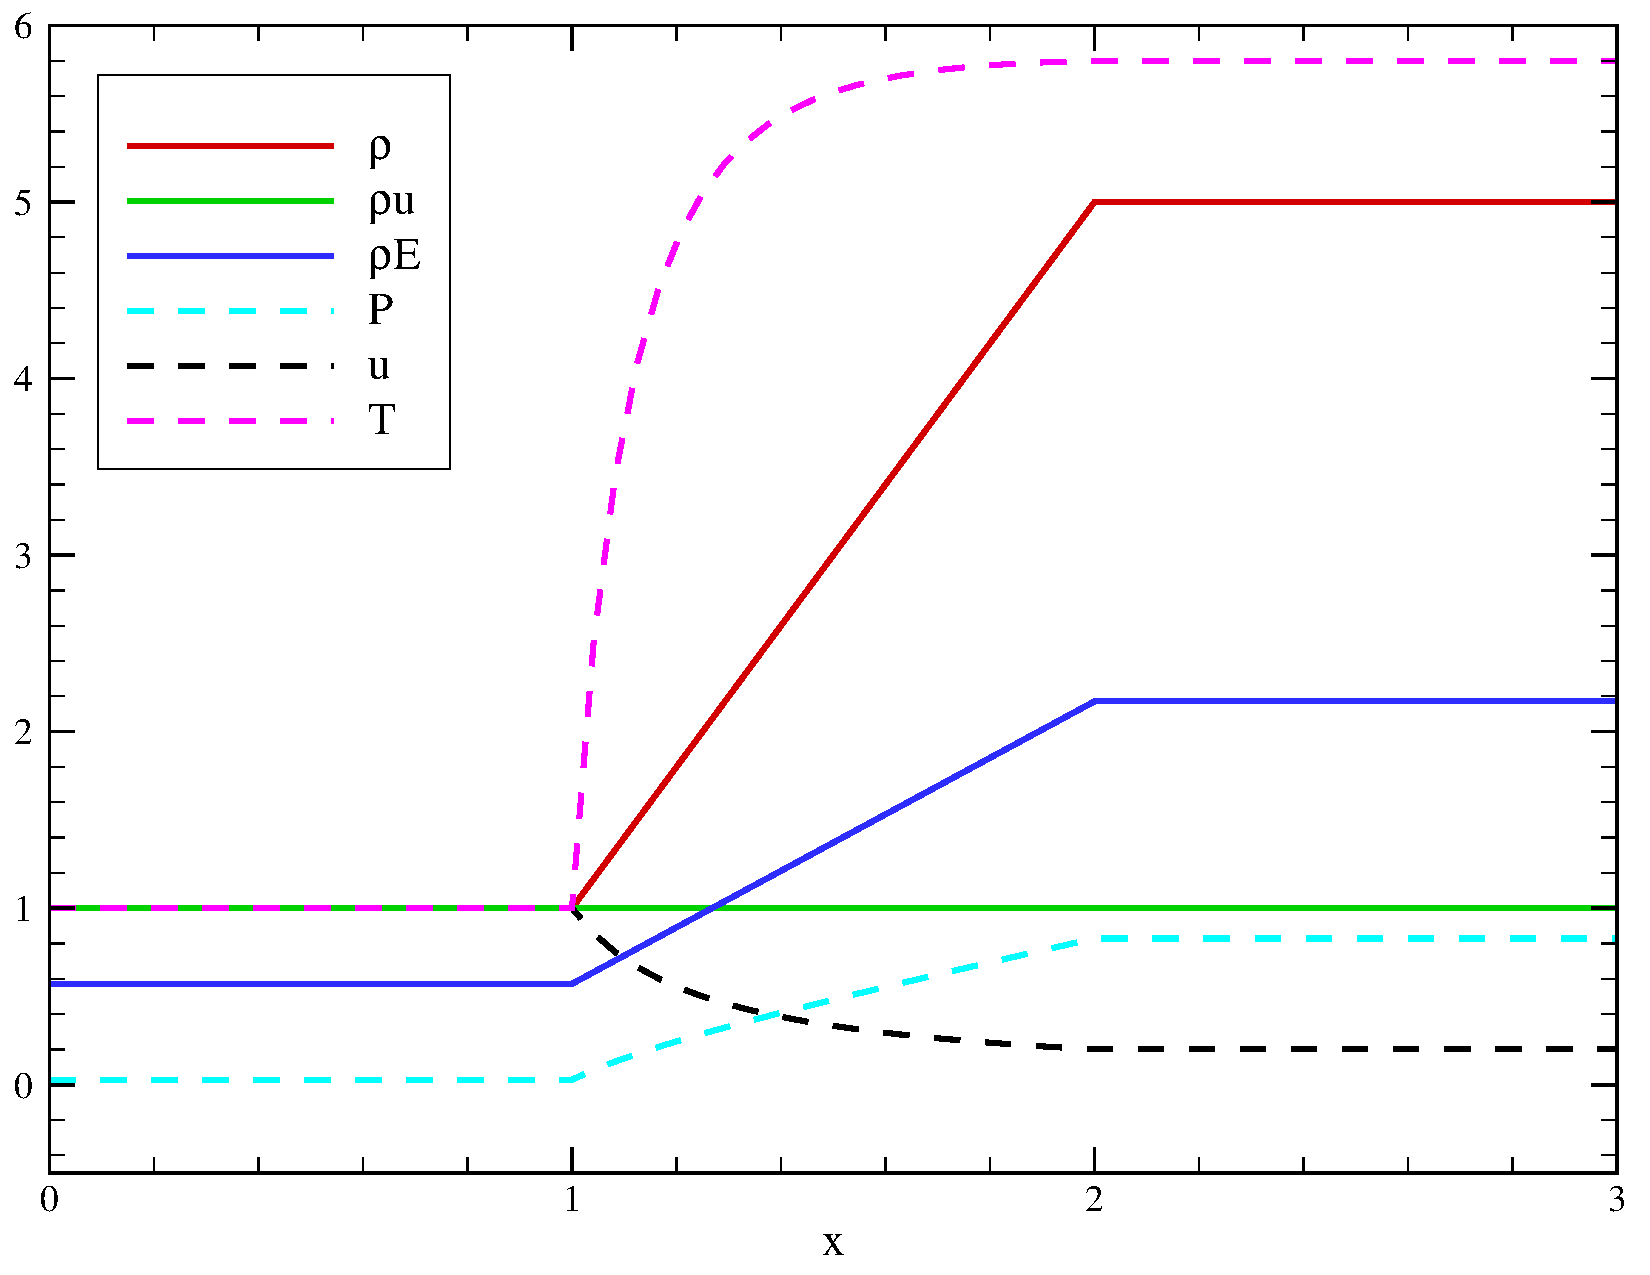
\includegraphics[height=.42\textheight]{figures/comp_ns_interpolation/primitive_vars}} \\
    \subfigure[Linearly interpolated and reconstructed inviscid flux vector components.\label{fig:comp_ns_1D_inv_flux}]{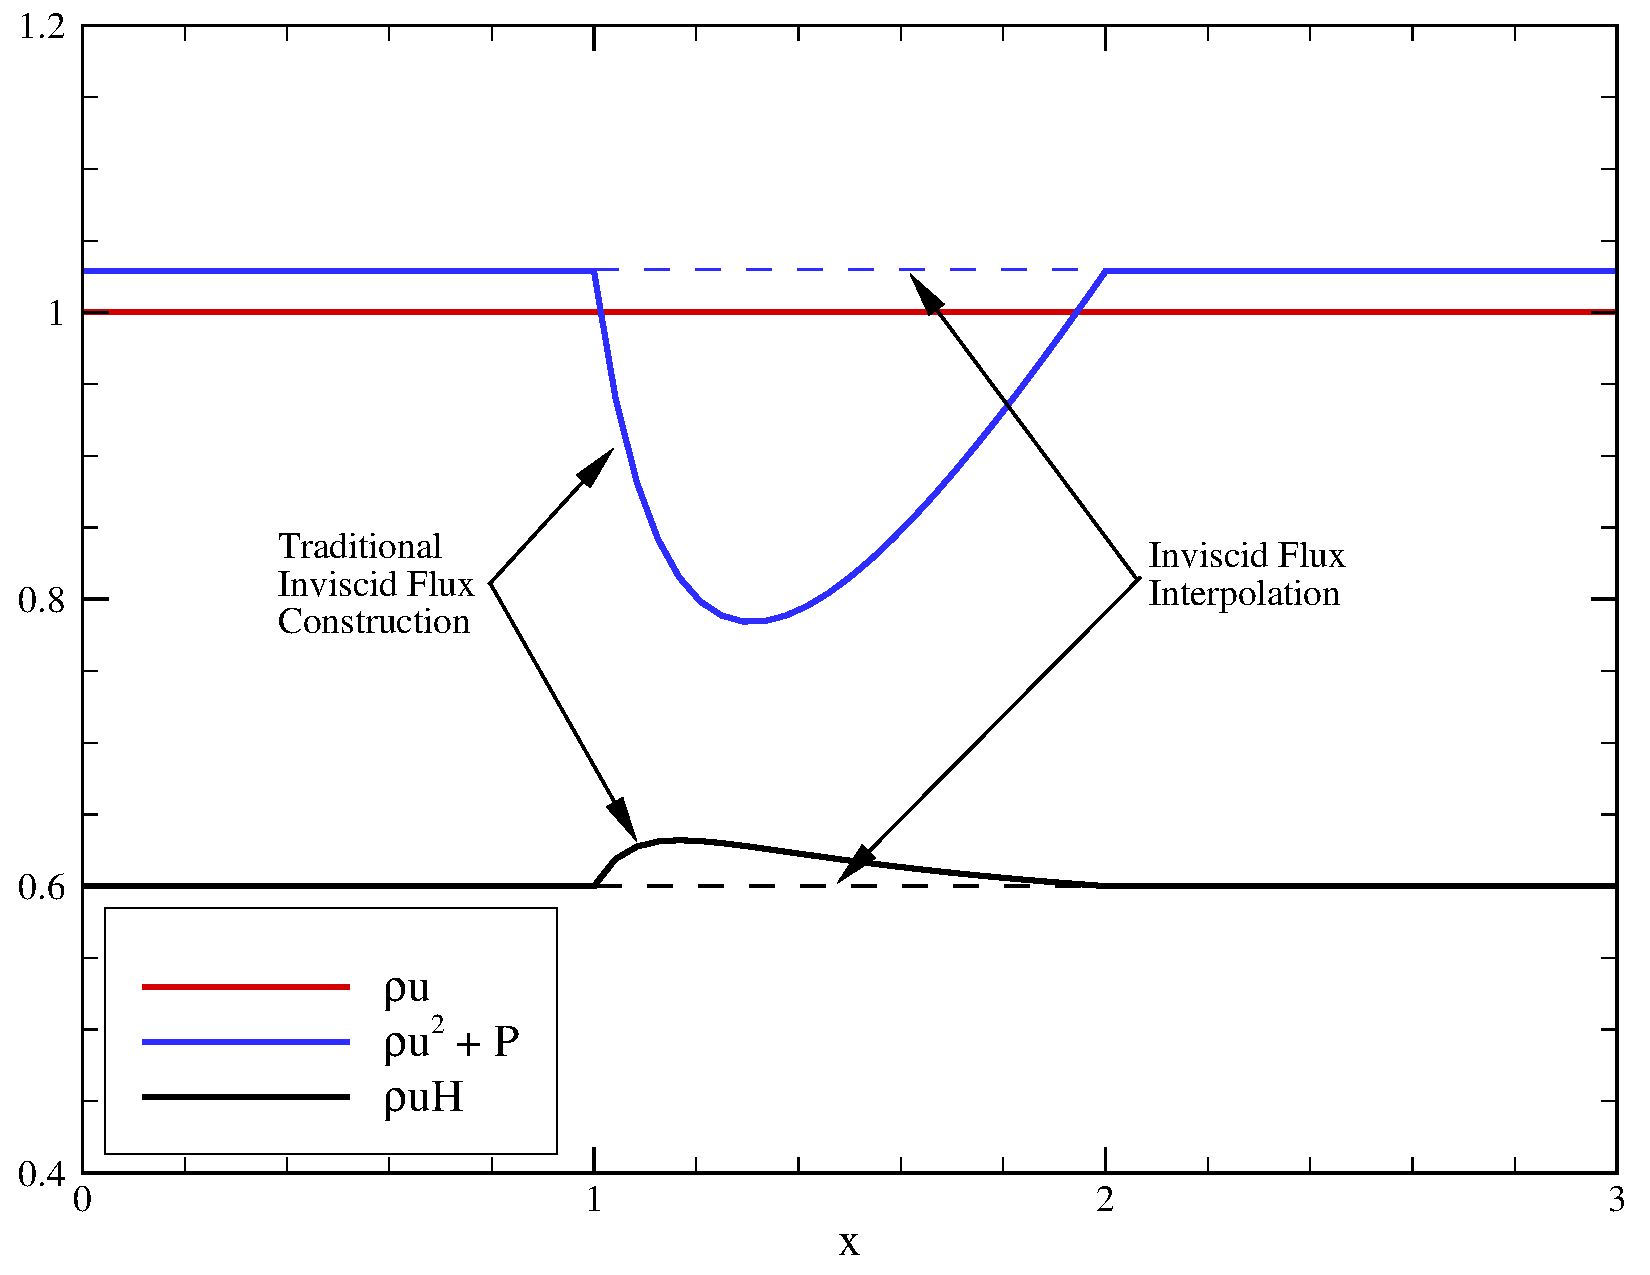
\includegraphics[height=.42\textheight]{figures/comp_ns_interpolation/inv_flux}}
    \caption{A steady normal shock at Mach~5 spanning three notional elements.\label{fig:comp_ns_m5_normal_shock}} 
  \end{center}
\end{figure}
The Figure considers a one-dimensional, inviscid, normal shock at Mach~5.  For this simple case the governing equations reduce to
\begin{align*}
  \pdv{\rho}{t} &+ \pdv{}{x} \left(\rho u\right) = 0 \\
  \pdv{\rho u}{t} &+ \pdv{}{x}\left(\rho u^2 + P\right) = 0 \\
  \pdv{\rho E}{t} &+ \pdv{}{x} \left(\rho u H\right) = 0
\end{align*}
and, at steady state, reduce to
\begin{equation}
  \pdv{}{x} \left(\rho u\right) = \pdv{}{x} \left(\rho u^2 + P\right) = \pdv{}{x} \left(\rho u H\right) \equiv 0 \label{eq:1d_steady_NS}
\end{equation}
which implies that $\rho u$, $\rho u^2+P$, and $\rho u H$ are all constant.

Figure~\ref{fig:comp_ns_cons_primitive} presents the scenario in which the exact solution is captured on three piecewise linear finite elements of unit length.  The solid lines in the figure depict the conserved variables for the nodally exact solution interpolated linearly in the finite element basis.  The dashed lines are the reconstructed primitive variables, which are highly nonlinear as they are in general rational functions of the conserved variables.  This is especially true in the case of the temperature, which has the form
\begin{equation*}
  T = \frac{e}{c_v} = \frac{\rho E - \frac{1}{2}\frac{\left(\rho u\right)^2}{\rho}}{\rho c_v} 
\end{equation*}

Figure~\ref{fig:comp_ns_1D_inv_flux} plots the inviscid flux vector components for both the traditional approach and the discretization given by~\eqref{eq:disc_F=AU_expanded}.  Note that for the traditional approach Equation~\eqref{eq:1d_steady_NS} is not satisfied within the element containing the shock, hence this scheme is incapable of representing the nodally exact solution.  By contrast, for the alternate choice of~\eqref{eq:disc_F=AU_expanded} Equation~\eqref{eq:1d_steady_NS} is satisfied exactly.

Recalling Equation~\eqref{eq:shock_capturing_parameter}, the inability to represent a nodally exact solution implies that the shock capturing operator will always be active in the traditional approach. The approach proposed here can satisfy the nodally exact solution and, therefore, is capable of converging to solutions in which $\delta$ vanishes throughout the domain.

Further, the distribution of $\left(\rho u^2 + P\right)$ and $\rho u H$ interior to the element containing the shock are of high-order for the traditional approach.  This is important because, in practice, the integrals in the finite element weak statement~\eqref{eq:comp_fe_SUPG_SC} are approximated using numerical quadrature, and this high-order behavior will not be evaluated exactly.

The fact that both schemes recover identical inviscid flux values at the nodes is also important.  This suggests that for a nodal quadrature rule both schemes should exhibit similar performance.  This conjecture is supported by recent work in which Kessler and Awruch consider an explicit Taylor--Galerkin finite element method for the Navier--Stokes equations in thermochemical nonequilibrium~\cite{hypersonic_taylor_galerkin}.  In this work the authors evaluate the element integrals a priori in closed-form using Gauss-Lobatto quadrature so that at each explicit time step costly numerical integration is avoided.  Given the behavior shown in Figure~\ref{fig:comp_ns_1D_inv_flux} their approach may have benefited from this enhanced stability by sampling the inviscid flux only at the element nodes.


%%%%%%%%%%%%%%%%%%%%%%%%%%%%%%%%%%%%%%%%%%%%%%%%%%%%%%%%%%%%%%%%%%%%%%%%%%%%%%%
%%%%%%%%%%%%%%%%%%%%%%%%%%%%%%%%%%%%%%%%%%%%%%%%%%%%%%%%%%%%%%%%%%%%%%%%%%%%%%%
\section{Solution Methodology\label{sec:comp_solution_methodology}}
Equations~\eqref{eq:comp_fe_SUPG_SC} form a transient, tightly coupled nonlinear system for the unknown nodal values $\bv{U}_h(\bv{x}_j,t)$.  Even when a steady solution to the governing equations is sought equations~\eqref{eq:comp_fe_SUPG_SC} are often solved with a pseudo-time continuation strategy.  That is, even for steady problems, the unsteady equations are often integrated in time until steady-state is reached.  This is especially the case for compressible flows containing shock waves because strong gradients which occur in the flow imply an extremely small zone of attraction for nonlinear solution schemes such as Newton's method. Algorithms for solving this type of transient system fall broadly into two categories: explicit and implicit.

Explicit algorithms are relatively straightforward to implement, but are not competitive for convection-dominated problems with non-negligible viscosity because of restrictive time step sizes which must be used.  Linear stability analysis for explicit schemes applied to the model convection-diffusion problem provides insight into time step stability. For convection processes the stable time step varies linearly with the mesh spacing, that is $\Delta t_\text{conv} \propto h$.  Analysis of the linear one-dimensional wave equation gives rise to the well-known Courant-Friedrichs-Lewy (CFL) condition, which states that for velocity $u$ and mesh size $h$ explicit stability requires $\frac{u \Delta t}{h} < 1$~\cite{cfmht}.   For diffusion processes the stable time step varies \emph{quadratically} with the mesh spacing, that is $\Delta t_\text{diff} \propto h^2$.   For the case of an inviscid flow this condition is irrelevant and the convective time step limit may not be overly-restrictive as the minimum mesh size $h$ may be relatively large.  For convection-dominated flows with thin boundary layers, however, the extremely fine mesh spacing at solid walls which is required to accurately resolve the boundary layer renders the explicit approach intractable. 

Implicit algorithms, by contrast, are substantially more expensive per time step, but have the advantage of avoiding stability limits on the size of time step used.  Since the present work seeks to use adaptive meshing techniques to locally resolve fine features of the flow (thus decreasing $h$), the $h$-dependence of $\Delta t$ for explicit schemes is particularly unattractive. The cost for this increased stability is the need to solve (at least approximately) a nonlinear implicit system at each time step of the solution.  Preconditioned Krylov subspace iterative methods provide a suitable choice of solvers that are amenable to parallel solution and are efficient for the problems of interest here.  

The remainder of this section describes (1) the time integration and (2) linearization strategies used for both steady-state and time accurate flows.  The iterative techniques used to solve the resulting linear systems will also be briefly discussed.

%%%%%%%%%%%%%%%%%%%%%%%%%%%%%%%%%%%%%%%%%%%%%%%%%%%%%%%%%%%%%%%%%%%%%%%%%%%%%%%
\subsection{Time Integration}
As mentioned previously, steady solutions are often found by time-marching the transient governing equations to steady-state.  In this sense the initial condition is taken at time $t=0$ and the solution is marched in time until $\pdv{\bv{U}}{t}\rightarrow 0$.  In this way time is essentially a continuation parameter which defines a sequence $(n=1,2,\ldots)$ of solutions $\bv{U}_n$ which converge to the steady solution $\bv{U}$. 

The semidiscrete weak form in Equation~\eqref{eq:comp_fe_SUPG_SC} is discretized in time using backwards finite difference schemes.  Both first and second-order accurate in time schemes may be derived from Taylor series expansions in time about $\bv{U}_h\left(t_{n+1}\right)=\bv{U}_{n+1}$:
\begin{align}
  \bv{U}_n     = \bv{U}_{n+1} &+ \pdv{\bv{U}_{n+1}}{t}\left(t_n-t_{n+1}\right) + \pdtwov{\bv{U}_{n+1}}{t}\frac{\left(t_n-t_{n+1}\right)^2}{2} \nonumber \\
                              &+ \mathcal{O}\left(\left(t_n-t_{n+1}\right)^3\right) \nonumber \\
                              & \nonumber \\
  \bv{U}_{n-1} = \bv{U}_{n+1} &+ \pdv{\bv{U}_{n+1}}{t}\left(t_{n-1}-t_{n+1}\right) + \pdtwov{\bv{U}_{n+1}}{t}\frac{\left(t_{n-1}-t_{n+1}\right)^2}{2} \nonumber \\
                              &+ \mathcal{O}\left(\left(t_{n-1}-t_{n+1}\right)^3\right) \nonumber
\end{align}
which, upon substituting $t_{n+1} - t_n\equiv\Delta t_{n+1}$ and $t_{n+1} - t_{n-1}=\Delta t_{n+1} + \Delta t_n$, becomes
\begin{align}
  \bv{U}_n     = \bv{U}_{n+1} &- \pdv{\bv{U}_{n+1}}{t}\Delta t_{n+1} + \pdtwov{\bv{U}_{n+1}}{t}\frac{\Delta t_{n+1}^2}{2} - \mathcal{O}\left(\Delta t_{n+1}^3\right) \nonumber \\ 
                              & \nonumber \\
  \bv{U}_{n-1} = \bv{U}_{n+1} &- \pdv{\bv{U}_{n+1}}{t}\left(\Delta t_{n+1}+\Delta t_n\right) + \pdtwov{\bv{U}_{n+1}}{t}\frac{\left(\Delta t_{n+1}+\Delta t_n\right)^2}{2} \nonumber \\
                              &- \mathcal{O}\left(\left(\Delta t_{n+1}+\Delta t_n\right)^3\right) \nonumber
\end{align}
which can be rewritten for $\pdv{\bv{U}_{n+1}}{t}$ as:
\begin{align}
  \pdv{\bv{U}_{n+1}}{t} = &\frac{\bv{U}_{n+1}}{\Delta t_{n+1}} - \frac{\bv{U}_n}{\Delta t_{n+1}} + \pdtwov{\bv{U}_{n+1}}{t} \frac{\Delta t_{n+1}}{2}
                          - \mathcal{O}\left(\Delta t_{n+1}^2\right) \label{eq:udot,un} \\
                              & \nonumber \\
  \pdv{\bv{U}_{n+1}}{t} = &\frac{\bv{U}_{n+1}}{\Delta t_{n+1} + \Delta t_n} - \frac{\bv{U}_{n-1}}{\Delta t_{n+1} + \Delta t_n} + \pdtwov{\bv{U}_{n+1}}{t}\frac{\left(\Delta t_{n+1} + \Delta t_n\right)}{2} \nonumber \\
                          &- \mathcal{O}\left(\left(\Delta t_{n+1} + \Delta t_n\right)^2\right) \label{eq:udot,unm1}
\end{align}


\subsubsection{Time Marching to Steady-State}
The familiar backward Euler time discretization follows directly from~\eqref{eq:udot,un} by recognizing
\begin{equation}
  \pdv{\bv{U}_{n+1}}{t} = \frac{\bv{U}_{n+1}}{\Delta t_{n+1}} - \frac{\bv{U}_n}{\Delta t_{n+1}} + \mathcal{O}\left(\Delta t_{n+1}\right)
  \label{eq:udot_backward_euler}
\end{equation}
which provides a first-order in time approximation upon neglecting the $\mathcal{O}\left(\Delta t_{n+1}\right)$ term.  As such, this scheme yields a fully implicit problem for $\bv{U}_{n+1}$ which may be used when time accuracy is not required.  

\subsubsection{Time-Accurate Flows}
A linear combination of~\eqref{eq:udot,un} scaled by $\left(1+\frac{\Delta t_{n+1}}{\Delta t_n}\right)$ and~\eqref{eq:udot,unm1} scaled by $-\frac{\Delta t_{n+1}}{\Delta t_n}$ can be used to annihilate the leading $\pdtwov{\bv{U}_{n+1}}{t}$ term and create a backward, second-order accurate approximation to $\pdv{\bv{U}_{n+1}}{t}$.  This approximation, along with~\eqref{eq:udot_backward_euler}, can be generalized in the form
\begin{equation}
  \pdv{\bv{U}_{n+1}}{t} = \alpha_t \bv{U}_{n+1} + \beta_t \bv{U}_n + \gamma_t \bv{U}_{n-1} + \mathcal{O}\left(\Delta t_{n+1}^p\right)
  \label{eq:udot_thee_pt_backward}
\end{equation}
to yield either a first or second-order accurate scheme.  The weights $\alpha_t, \beta_t$, and $\gamma_t$ are given for $p=1$ and $p=2$ in Table~\ref{table:udot_weights}.
\begin{table}[hbtp]
  \begin{center}
    \caption{First and second-order accurate time discretization coefficients.\label{table:udot_weights}}
    \vspace{1em}
    \large
    \begin{tabular}{c||ccc}
      $\bv{p}$ & $\bv{\alpha_t}$ & $\bv{\beta_t}$ & $\bv{\gamma_t}$ \\ \hline\hline
          &          &         & \\
       1  & $\frac{1}{\Delta t_{n+1}}$ & $\frac{-1}{\Delta t_{n+1}}$ & 0 \\
          &          &         & \\
       2  & $-\beta_t - \gamma_t$ %$\left[\frac{1}{\Delta t_{n+1}} + \frac{1}{\Delta t_n} - \frac{\Delta t_{n+1}}{\Delta t_n\left(\Delta t_n+1 + \Delta t_n\right)}\right]$ 
          & $-\left[\frac{1}{\Delta t_{n+1}} + \frac{1}{\Delta t_n}\right]$
          & $\frac{\Delta t_{n+1}}{\Delta t_n\left(\Delta t_{n+1} + \Delta t_n\right)}$ 
    \end{tabular}
  \end{center}
\end{table}
Since this second-order scheme requires \emph{two} levels of solution history it is not self-starting.  In practice ten backwards Euler steps are taken to develop the required  solution history and to allow rapid transients to subside before applying the second-order scheme.


%%%%%%%%%%%%%%%%%%%%%%%%%%%%%%%%%%%%%%%%%%%%%%%%%%%%%%%%%%%%%%%%%%%%%%%%%%%%%%%
\subsection{Linearization}
After time discretization using either~\eqref{eq:udot_backward_euler} or~\eqref{eq:udot_thee_pt_backward}, Equation~\eqref{eq:comp_fe_SUPG_SC} can be written in residual form for the unknown nodal values $\bv{U}_{n+1}\equiv\bv{U}_h\left(t_{n+1}\right)$ as the nonlinear algebraic system
\begin{equation}
  \label{eq:comp_residual}  
  \bv{R}\left(\bv{U}_{n+1}\right) = 0 
\end{equation}
The goal of this section is to define a sequence of linear problems that, when solved, converge to obtain the solution $\bv{U}_{n+1}$ of the nonlinear system~\eqref{eq:comp_residual}.

%%%%%%%%%%%%%%%%%%%%%%%%%%%%%%%%%%%%%%%%%%%%%%%%%%%%%%%%%%%%%%%%%%%%%%%%%%%%%%%
\subsubsection{Newton Scheme}
 Expanding~\eqref{eq:comp_residual} with a Taylor series about iterate $\bv{U}_{n+1}^l$ gives
\begin{equation}
  \label{eq:comp_residual_linearized}  
  \bv{R}\left(\bv{U}_{n+1}^{l+1}\right) = \bv{R}\left(\bv{U}_{n+1}^l\right) +\left[\pdv{\bv{R}\left(\bv{U}_{n+1}^l\right)}{\bv{U}_{n+1}}\right]\;\delta\bv{U}_{n+1}^{l+1} + \mathcal{O}\left(\left(\delta\bv{U}_{n+1}^{l+1}\right)^2\right)
\end{equation}
where $\pdv{\bv{R}}{\bv{U}}$ is the Jacobian matrix for the nonlinear system and $\delta \bv{U}_{n+1}^{l+1}=\bv{U}_{n+1}^{l+1}-\bv{U}_{n+1}^l$. Truncating this expansion and setting $\bv{R}\left(\bv{U}_{n+1}^{l+1}\right)=0$ yields Newton's method
\begin{align}
  0 &= \bv{R}\left(\bv{U}_{n+1}^l\right) + \left[\pdv{\bv{R}\left(\bv{U}_{n+1}^l\right)}{\bv{U}_{n+1}}\right]\;\delta\bv{U}_{n+1}^{l+1} \nonumber \\
  \left[\pdv{\bv{R}\left(\bv{U}_{n+1}^l\right)}{\bv{U}_{n+1}}\right]\;\delta\bv{U}_{n+1}^{l+1} &= -\bv{R}\left(\bv{U}_{n+1}^l\right) \label{eq:comp_newton_system}
\end{align}
which results in an implicit linear system for $\delta\bv{U}_{n+1}^{l+1}$ and a sequence of iterates $(l=0,1,\ldots)$ which converges to $\bv{U}_{n+1}$.  It is important to recall than Newton's method exhibits second-order \emph{conditional} convergence. That is, the magnitude of $\bv{R}\left(\bv{U}_{n+1}^{l+1}\right)$ decreases quadratically at successive iterates provided that the initial guess $\bv{U}_{n+1}^0$ is ``sufficiently close'' to the unknown $\bv{U}_{n+1}$~\cite{iserles_numerical_analysis,greenberg_applied_math}.

While the full-Newton scheme is conceptually simple the implementation is complicated by the nonlinear dependence of the transport properties on the unknowns (see Equation~\eqref{eq:sutherland}) and the highly nonlinear nature of the convective terms themselves.  In practice, implementing the full-Newton scheme is computationally intensive and, in the case of supersonic flows exhibiting shock waves, is often only of modest benefit.  That is, due to the conditional convergence restriction of the method and the sharp gradients or discontinuities which are present in the flowfield, the asymptotic quadratic convergence rate may not be achieved~\cite{johan_hughes_shakib_mf}. The implementation of an approximate Newton-Krylov technique to address these issues will be discussed further in Section~\ref{sec:comp_linsolve_mf}.  

%%%%%%%%%%%%%%%%%%%%%%%%%%%%%%%%%%%%%%%%%%%%%%%%%%%%%%%%%%%%%%%%%%%%%%%%%%%%%%%
\subsubsection{Frozen Coefficient Scheme}
The frozen coefficient scheme form results when the coefficient matrices in~\eqref{eq:comp_fe_SUPG_SC} are evaluated using the last solution in a successive approximation nonlinear iteration.  This approach allows the linear system to be assembled easily at each nonlinear step and is computationally attractive.

However, numerical experiments show erratic convergence for this approach.  For example, nonlinear convergence stagnates and  the magnitude of the time derivative $\|\pdv{\bv{U}}{t}\|$ stops decreasing at some finite value.  Shakib et al.~\cite{johan_hughes_shakib_mf} point out that the frozen coefficient scheme does not necessarily yield a descent direction for $\bv{R}\left(\bv{U}\right)$.  That is, each successive iterate is not guaranteed to produce a solution which reduces the residual.  Bearing this in mind, this convergence stagnation is not surprising.  It is simply the price to pay for considering an incomplete Jacobian approximation of~\eqref{eq:comp_residual_linearized}. Similar convergence stagnation has been observed in the finite volume community when particular flux limiters are used.

A practical solution to this problem has recently been proposed by Catabriga and Coutinho~\cite{catabriga_coutinho_SUPG_convergence}.  The solution proposed by Catabriga and Coutinho in the context of steady flows is to ``freeze'' the shock capturing parameter at some point in the computation.  The nonlinear solution then proceeds with $\delta$ fixed at some previous value and the scheme will typically converge to machine precision.

%%%%%%%%%%%%%%%%%%%%%%%%%%%%%%%%%%%%%%%%%%%%%%%%%%%%%%%%%%%%%%%%%%%%%%%%%%%%%%%
\subsection{Linear System Solution Scheme}
Both the Newton and frozen coefficient Jacobian schemes result in a series of sparse linear problems of the form
\begin{equation}
  \bt{K}\;\delta\bv{U}_{n+1}=\bv{f}
  \label{eq:comp_linsolve_sys}
\end{equation}
which must be solved to obtain $\bv{U}_{n+1}$.  For the discretization presented in Section~\ref{sect:comp_fe_formulation} using standard piecewise-linear elements $\bt{K}$ is a non-symmetric, sparse, non-singular $\left(nv\times n_{\text{nodes}}\right)\times\left(nv\times n_{\text{nodes}}\right)$ real matrix where $n_{\text{nodes}}$ is the total number of nodes in the mesh and $nv$ is the number of unknowns per node (which is equal to four in two dimensions and five in three dimensions).  Given the size and sparseness of $\bt{K}$ it is natural to use preconditioned Krylov subspace iterative techniques to approximate $\delta\bv{U}_{n+1}$~\cite{barrett94templates,golub_van_loan}.  The essential kernel of these techniques is the computation of the matrix-vector product $\bv{y}=\bt{K}\;\bv{x}$.  Two techniques for providing this kernel will be discussed, the first stores the sparse matrix and computes the matrix-vector product explicitly; the second computes the action of the matrix-vector product in a ``matrix-free'' sense.

%%%%%%%%%%%%%%%%%%%%%%%%%%%%%%%%%%%%%%%%%%%%%%%%%%%%%%%%%%%%%%%%%%%%%%%%%%%%%%%
\subsubsection{Sparse Matrix Approach}
One straightforward technique for solving~\eqref{eq:comp_linsolve_sys} is to build the system matrix $\bt{K}$ and right-hand-side vector $\bv{f}$.  Since the matrix is large yet sparse care must be taken to store it efficiently.  In the present work the parallel sparse matrix format implemented in the PETSc toolkit is used, as are the PETSc iterative solvers~\cite{petsc_manual}.  When the system matrix is constructed explicitly it may then be copied and modified to serve as a preconditioner as well.  (This is the approach used in this work.)  In the current work a standard parallel block-Jacobi ILU-0 preconditioner is used~\cite{barrett94templates,golub_van_loan}.  Once the system matrix and preconditioner are formed the required matrix-vector products are computed directly.


%%%%%%%%%%%%%%%%%%%%%%%%%%%%%%%%%%%%%%%%%%%%%%%%%%%%%%%%%%%%%%%%%%%%%%%%%%%%%%%
\subsubsection{Matrix-Free Approach\label{sec:comp_linsolve_mf}}
Recall from Equation~\eqref{eq:comp_newton_system} the particular form of the implicit system to be solved:
\begin{equation*}
  \left[\pdv{\bv{R}}{\bv{U}}\right]\;\delta\bv{U} = -\bv{R}\left(\bv{U}\right)
\end{equation*}
For this special case the action of the matrix-vector product $\left[\pdv{\bv{R}}{\bv{U}}\right]\;\delta\bv{U}$ is nothing more than the derivative of $\bv{R}$ in the direction specified by $\delta\bv{U}$, which is formally defined as
\begin{equation*}
  \left[\pdv{\bv{R}}{\bv{U}}\right]\;\delta\bv{U} \equiv \lim_{\varepsilon\rightarrow 0} \left\{\frac{\bv{R}\left(\bv{U} + \varepsilon \delta \bv{U}\right) - \bv{R}\left(\bv{U}\right)}{\varepsilon}\right\}
\end{equation*}
and may be approximated within $\mathcal{O}\left(\varepsilon\right)$ for finite~$\varepsilon$ as
\begin{equation}
  \left[\pdv{\bv{R}}{\bv{U}}\right]\;\delta\bv{U} \approx \frac{\bv{R}\left(\bv{U} + \varepsilon \delta \bv{U}\right) - \bv{R}\left(\bv{U}\right)}{\varepsilon}
  \label{eq:comp_linsolve_mf}
\end{equation}
From Equation~\eqref{eq:comp_linsolve_mf} it is clear that the required matrix-vector product may be approximated by differencing successive residual evaluations.  It is in this sense that the scheme is matrix-free: the actual system matrix need not be explicitly formed.  All that is required is the capability to evaluate the discrete residual $\bv{R}\left(\bv{U}\right)$.  Of course, for practical applications some form of preconditioning must be applied to the linear system. Depending on the implementation of this preconditioning the composite scheme may store some approximation of the system matrix.  Still, one attractive feature of the matrix-free approach is that it can require substantially less memory than the sparse matrix approach.

Perhaps the most compelling reason to use the matrix-free approach is that it directly yields a quasi-Newton formulation.  That is, the finite difference approximation properly accounts for \emph{all} the nonlinearities in the system.  This is especially attractive from an algorithm development perspective.  For example, alternate shock capturing terms, SUPG weighting functions, equations of state, and transport property definitions can all be implemented simply by defining their contribution to the discrete residual. Their contribution to the quasi-Newton iteration simply falls out through the approximate matrix-vector product~\eqref{eq:comp_linsolve_mf}.

The choice of $\varepsilon$ is critical for the success of the method and has been the subject of much research and will not be discussed in detail.  The primary concern is achieving $\varepsilon$ sufficiently small that~\eqref{eq:comp_linsolve_mf} is reasonably accurate while avoiding catastrophic cancellation which may occur when evaluating the numerator with finite precision arithmetic~\cite{johan_hughes_shakib_mf}.  However, it is worth mentioning that an alternate approach for approximating the directional derivative is available (using complex arithmetic) which is second-order accurate in~$\varepsilon$, poses no risk for cancellation errors, and is of similar cost .  A simple Taylor series for a real valued function $f\left(x\right)$ evaluated for the complex perturbation $\left(x+i\,\varepsilon\right)$ gives
\begin{equation*}
  \frac{df}{dx} = \frac{\Im\left[f\left(x+i\,\varepsilon\right)\right]}{\varepsilon} + \mathcal{O}\left(\varepsilon^2\right)
\end{equation*}
where $\Im[]$ denotes the imaginary part of a complex number.  This robust technique has recently been applied by Nielsen and Kleb as a method for computing discrete adjoint operators for a finite volume formulation of the Navier-Stokes equations on unstructured meshes~\cite{nielsen_kleb_2005}.  Future work will consider this technique in the context of matrix-free Newton-Krylov methods as an alternate approach for constructing an approximate Jacobian matrix.

%%%%%%%%%%%%%%%%%%%%%%%%%%%%%%%%%%%%%%%%%%%%%%%%%%%%%%%%%%%%%%%%%%%%%%%%%%%%%%%
\subsection{Adaptive Mesh Refinement\label{sec:comp_ns_amr}}

The adaptive solution techniques discussed in the previous chapters may be applied to great effect for the case of supersonic compressible flows.  As mentioned in the introductory remarks of this chapter, this class of flows is characterized by highly localized features.  Shock waves which may occur are physically on the order of several molecular mean-free paths wide (on the order of micrometers for air at sea level conditions).  Compared to the scale of flight vehicles, these shock waves appear essentially as discontinuities.  Further, their precise location is not known a priori, so it is natural to use an adaptive technique to accurately capture these features.

The boundary layer adjacent to solid surfaces in viscous flows is another region of very high gradients which occur in a small region of the domain.  Typical practice for aerodynamic and aerothermodynamic applications is to construct a computational mesh which is expected to capture these features accurately. Viscous shear layers pose a similar but more complex problem in that their precise location is not known during the mesh generation process. For cases involving complicated and/or transient features such as shock wave/boundary layer interaction, this mesh generation technique necessarily becomes an iterative one.

Adaptive mesh refinement allows an alternative to this cumbersome iterative solution procedure by embedding the mesh improvement process directly in the application code.  In the numerical examples which follow these adaptive techniques will be used to provide local resolution for strong shock waves which occur in both viscous and inviscid flows.  Additionally, the technique is applied to viscous/inviscid interactions and complex shock-shock interactions to assess their viability for performing aerothermodynamic applications.

The solution procedure with adaptive mesh refinement is largely the same as described in Chapter~\ref{chap:bio}.  One significant departure here is that in some cases `feature indicators' are used as an alternative means for selecting which portions of the domain are to be refined.  This feature-based approach does not enjoy the rigorous theoretical support of true error estimation techniques, but has worked well in practice for a number of applications (as will be demonstrated).


%%%%%%%%%%%%%%%%%%%%%%%%%%%%%%%%%%%%%%%%%%%%%%%%%%%%%%%%%%%%%%%%%%%%%%%%%%%%%%%
%\clearpage
\subsection{Solution Algorithm}
The solution methodologies described in the previous sections are combined into the transient adaptive nonlinear solution algorithm listed as Algorithm~\ref{alg:comp_ns_algorithm}.
\begin{algorithm}[!htb]
  \centering
  \begin{minipage}{.95\textwidth}
    \caption{Transient adaptive nonlinear solution algorithm used for compressible flow applications\label{alg:comp_ns_algorithm}}
    \noindent
    \sffamily
    \setcounter{alines}{0}
    \begin{list}{\arabic{alines}:\ \ }{\usecounter{alines}}
        \renewcommand{\baselinestretch}{1.0} \setlength{\itemsep}{-1ex}
        \item Interpolate initial conditions
	\item $\bv{U}_0 = \bv{U}(\bv{x},t)$ 
        \item \textbf{for} $n=1$ to $N_\text{time steps}$ \textbf{do}
	\item \ \ \ Let $\hat{\bv{U}}_n = \bv{U}_{n-1}$
	\item \ \ \ Solve the nonlinear system for $\hat{\bv{U}}_n$:
 	\item \ \ \ \textbf{do}
 	\item \ \ \ \ \ \ Form system matrix $\bt{K} = \bt{K}(\hat{\bv{U}}_n)$
 	\item \ \ \ \ \ \ Form system vector $\bv{f}= \bv{f}(\hat{\bv{U}}_n,\bv{U}_{n-1},\bv{U}_{n-2})$
 	\item \ \ \ \ \ \ Solve the linear system $\bt{K} \; \delta\hat{\bv{U}}_n = \bv{f}$
	\item \ \ \ \ \ \ Update the solution $\hat{\bv{U}}_n \leftarrow \hat{\bv{U}}_n + \delta\hat{\bv{U}}_n$
 	\item \ \ \ \textbf{while} $\norm[\infty]{\delta\hat{\bv{U}}_n} < \varepsilon_{nl}$
	\item \ \ \ Compute error indicator for each element using $\hat{\bv{U}}_n$
	\item \ \ \ \textbf{if} error is acceptable
	\item \ \ \ \ \ \ Let $\bv{U}_n=\hat{\bv{U}}_n$
        \item \ \ \ \textbf{else}
	\item \ \ \ \ \ \ Refine and coarsen mesh
	\item \ \ \ \ \ \ Project $\Pi\hat{\bv{U}}_n\rightarrow\bv{U}_n$
	\item \ \ \ \ \ \ Solve the nonlinear system for $\bv{U}_n$:
 	\item \ \ \ \ \ \ \textbf{do}
 	\item \ \ \ \ \ \ \ \ \ Form system matrix $\bt{K} = \bt{K}(\bv{U}_n)$
 	\item \ \ \ \ \ \ \ \ \ Form system vector $\bv{f}= \bv{f}(\bv{U}_n,\bv{U}_{n-1},\bv{U}_{n-2})$
 	\item \ \ \ \ \ \ \ \ \ Solve the linear system $\bt{K} \; \delta\bv{U}_n = \bv{f}$
	\item \ \ \ \ \ \ \ \ \ Update the solution $\bv{U}_n \leftarrow \bv{U}_n + \delta\bv{U}_n$
 	\item \ \ \ \ \ \ \textbf{while} $\norm[\infty]{\delta\bv{U}_n} < \varepsilon_{nl}$
        \item \ \ \ \textbf{endif}
        \item \textbf{end} \\
    \end{list}
  \end{minipage}
\end{algorithm}
This is the algorithm that is used to perform the application studies presented in the next section.

%%%%%%%%%%%%%%%%%%%%%%%%%%%%%%%%%%%%%%%%%%%%%%%%%%%%%%%%%%%%%%%%%%%%%%%%%%%%%%%
%%%%%%%%%%%%%%%%%%%%%%%%%%%%%%%%%%%%%%%%%%%%%%%%%%%%%%%%%%%%%%%%%%%%%%%%%%%%%%%
\clearpage
\section{Application Studies\label{chap:compressible:applications}}
This section presents a number of application studies designed to test various aspects of the finite element algorithm described in Section~\ref{sect:comp_fe_formulation} which is used to solve equations~\eqref{eq:pde_comp_mass}--\eqref{eq:pde_comp_energy}.  The application code used for these studies is built on top of the \texttt{libMesh}\footnote{\url{http://libmesh.sourceforge.net}} parallel adaptive finite element library and uses a fully implicit scheme to solve the weak formulation presented in~\eqref{eq:comp_weak_SUPG_SC}.  The problems considered here are generally hypersonic, laminar, perfect gas flows in two and three dimensions.

The applications are run on computational resources ranging from desktop machines to workgroup-class parallel clusters to the \emph{Columbia} supercomputer.  All computations employ the PETSc toolkit from Argonne National Laboratory~\cite{petsc_manual} to solve the parallel implicit linear systems using the generalized minimum residual (GMRES) Krylov subspace technique~\cite{saad_schultz_gmres} with preconditioning.  The preconditioner is of parallel block Jacobi-type where each processor sub-block uses an overlapping additive Schwartz method with an incomplete lower-upper factorization at the sub-block level with no fill (ILU-0).  Spatial integration is performed with Gauss quadrature rules sufficient to integrate 3\textsuperscript{rd}--order polynomials exactly.

The first applications will focus on the numerical aspects of the present finite element algorithm, investigating issues such as accuracy, efficiency, and convergence.  More difficult applications are then selected for phenomenological study and to demonstrate the broad applicability of the scheme, particularly to the case of steady and unsteady hypersonic aerothermodynamics.

%%%%%%%%%%%%%%%%%%%%%%%%%%%%%%%%%%%%%%%%%%%%%%%%%%%%%%%%%%%%%%%%%%%%%%%%%%%%%%%
\clearpage
\subsection{Inviscid Flow over a Cylinder\label{sec:comp_ns_cyl}}
\subsubsection{Geometry and Flow Conditions}
Two-dimensional inviscid Mach~3 flow over a circular cylinder is an established benchmark problem~\cite{jang_shu_weno_JCP,shu_fd_fv_dg_icase} and is studied here to investigate the performance of the implicit formulation.  The exterior flow problem is posed on a finite subdomain with uniform far-field data prescribed on the inflow boundary.  The computational grid for this case is mapped from the unit square $\left[0,1\right]\times\left[0,1\right]$ in the $\left(\xi,\eta\right)$ plane by
\begin{align}
  x(\xi,\eta) &= \left(R_x - \left(R_x - R_c\right)\xi\right) \cos\left(\theta\left(2\eta - 1\right)\right) \\
  y(\xi,\eta) &= \left(R_y - \left(R_y - R_c\right)\xi\right) \sin\left(\theta\left(2\eta - 1\right)\right) 
\end{align}
where the cylinder radius $R_c=0.5$, the upstream boundary of the computational domain is given by $R_x=1.5$, $R_y=3$, and $\theta=\frac{5\pi}{12}$.  A coarse mesh is shown in Figure~\ref{fig:cyl_grid_30x40} with $n_\xi\times n_\eta=30\times 40$ elements in the normal and circumferential directions, respectively.  The particular form of this mapping has been used in high-order finite difference discretizations as it yields a smooth, differentiable  mapping from computational to physical space~\cite{shu_fd_fv_dg_icase}.
\begin{figure}[hbtp]
  \begin{center}
    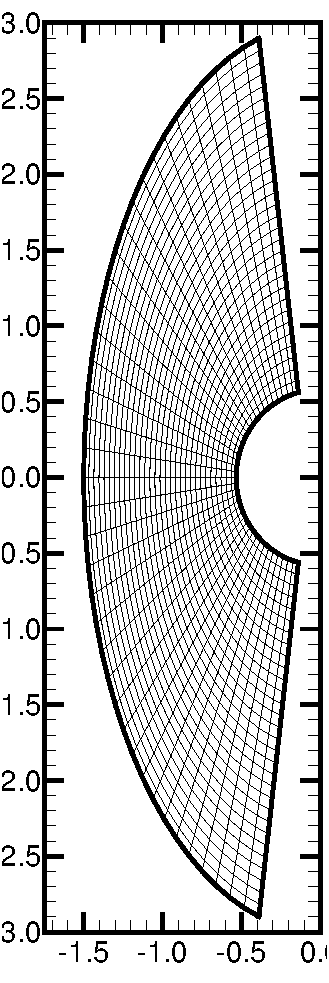
\includegraphics[height=0.8\textheight]{figures/mach3_cylinder/grid_30x40}
    \caption{Coarse computational grid for Mach~3 flow over a cylinder\label{fig:cyl_grid_30x40}}
  \end{center}
\end{figure}

The simulation is initialized with uniform freestream values and marched in time until steady--state is reached.  The upstream inflow boundary uses a supersonic  boundary condition in which the conserved variables $\left[\rho, \rho u, \rho v, \rho E\right]^T$ are specified as essential boundary conditions. The downstream outflow for this case is supersonic, and hence no outflow boundary conditions are specified for this inviscid flow.  The no--penetration boundary condition~$\bv{u}\cdot\nhat=0$ holds on the cylinder surface and is enforced as a natural boundary condition through the boundary integral in the weak statement as described in Section~\ref{sect:comp_ns_bcs}.

This example will be treated as a prototype for convection-dominated supersonic and hypersonic problems which arise in aerospace engineering.  The performance of the finite element algorithm presented in the previous sections will be examined in detail for this example.  The results of the numerical experiments performed in this section will be generalized and applied to more physically complicated flow phenomena in later sections.

\subsubsection{Flowfield and Stagnation Line Properties}
Figure~\ref{fig:cyl_flowfield} illustrates the steady-state flowfield for this case.  For this inviscid case the governing Euler equations~\eqref{eq:pde_comp_euler} are hyperbolic and admit discontinuous solutions. As expected, the cylinder produces a strong bow shock across which the density, velocity, and pressure jump, as predicted by the Rankine--Hugoniot equations (see Appendix~\ref{rankine_hugoniot_jumps}). 

% Cylinder flow contours
\begin{figure}[hbtp]
  \begin{center}
    \subfigure[Pressure   \label{fig:cyl_pressure}]{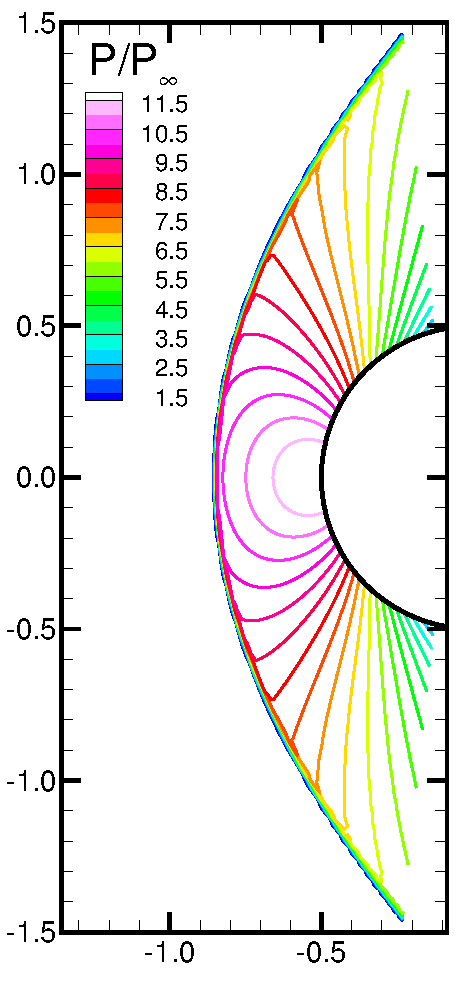
\includegraphics[width=0.25\textwidth]{figures/mach3_cylinder/P}}
    \subfigure[Density    \label{fig:cyl_density} ]{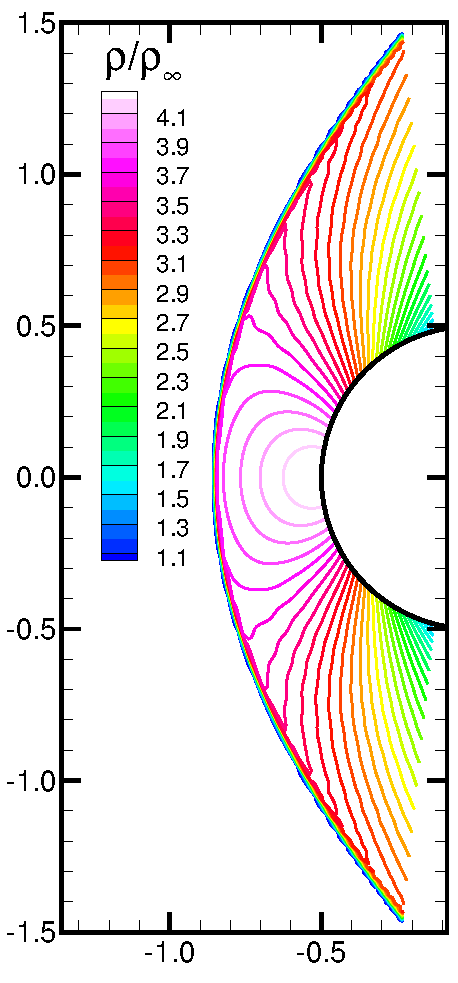
\includegraphics[width=0.25\textwidth]{figures/mach3_cylinder/rho}} \\
    \subfigure[Temperature\label{fig:cyl_temp}    ]{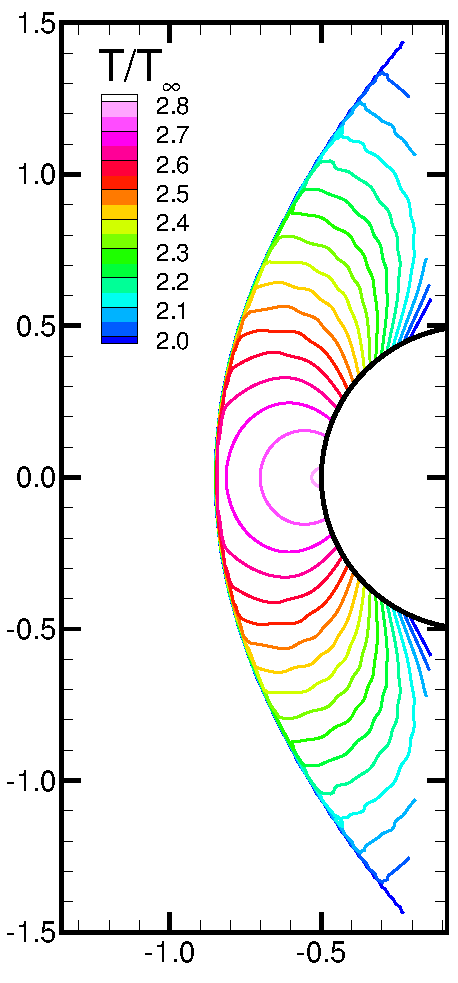
\includegraphics[width=0.25\textwidth]{figures/mach3_cylinder/T}}
    \subfigure[Mach Number\label{fig:cyl_mach}    ]{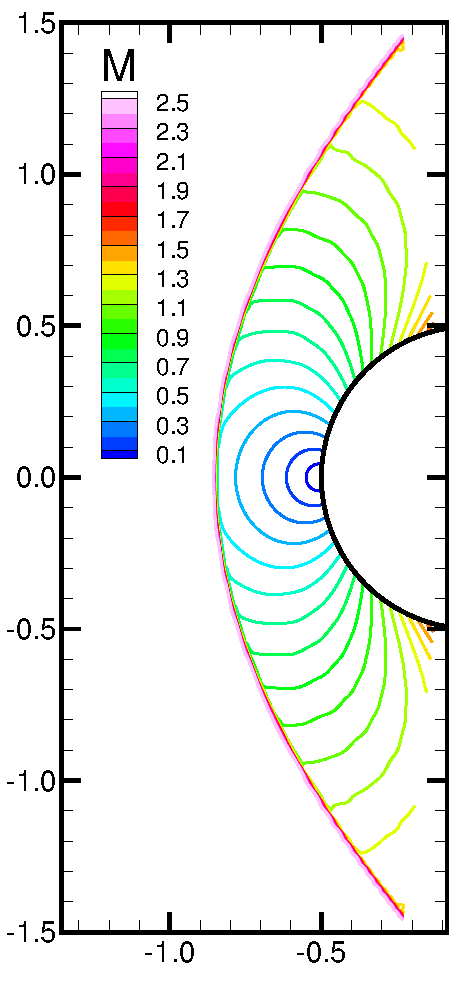
\includegraphics[width=0.25\textwidth]{figures/mach3_cylinder/M}}
    \caption{Illustration of flowfield for Mach~3 flow over a cylinder\label{fig:cyl_flowfield}}
  \end{center}
\end{figure}

Figure~\ref{fig:cyl_stagline} shows the flowfield properties along the stagnation line versus nondimensional distance x$/\text{R}_\text{N}$.  
% Stagnation line properties
\begin{figure}[hbtp]
  \begin{center}
    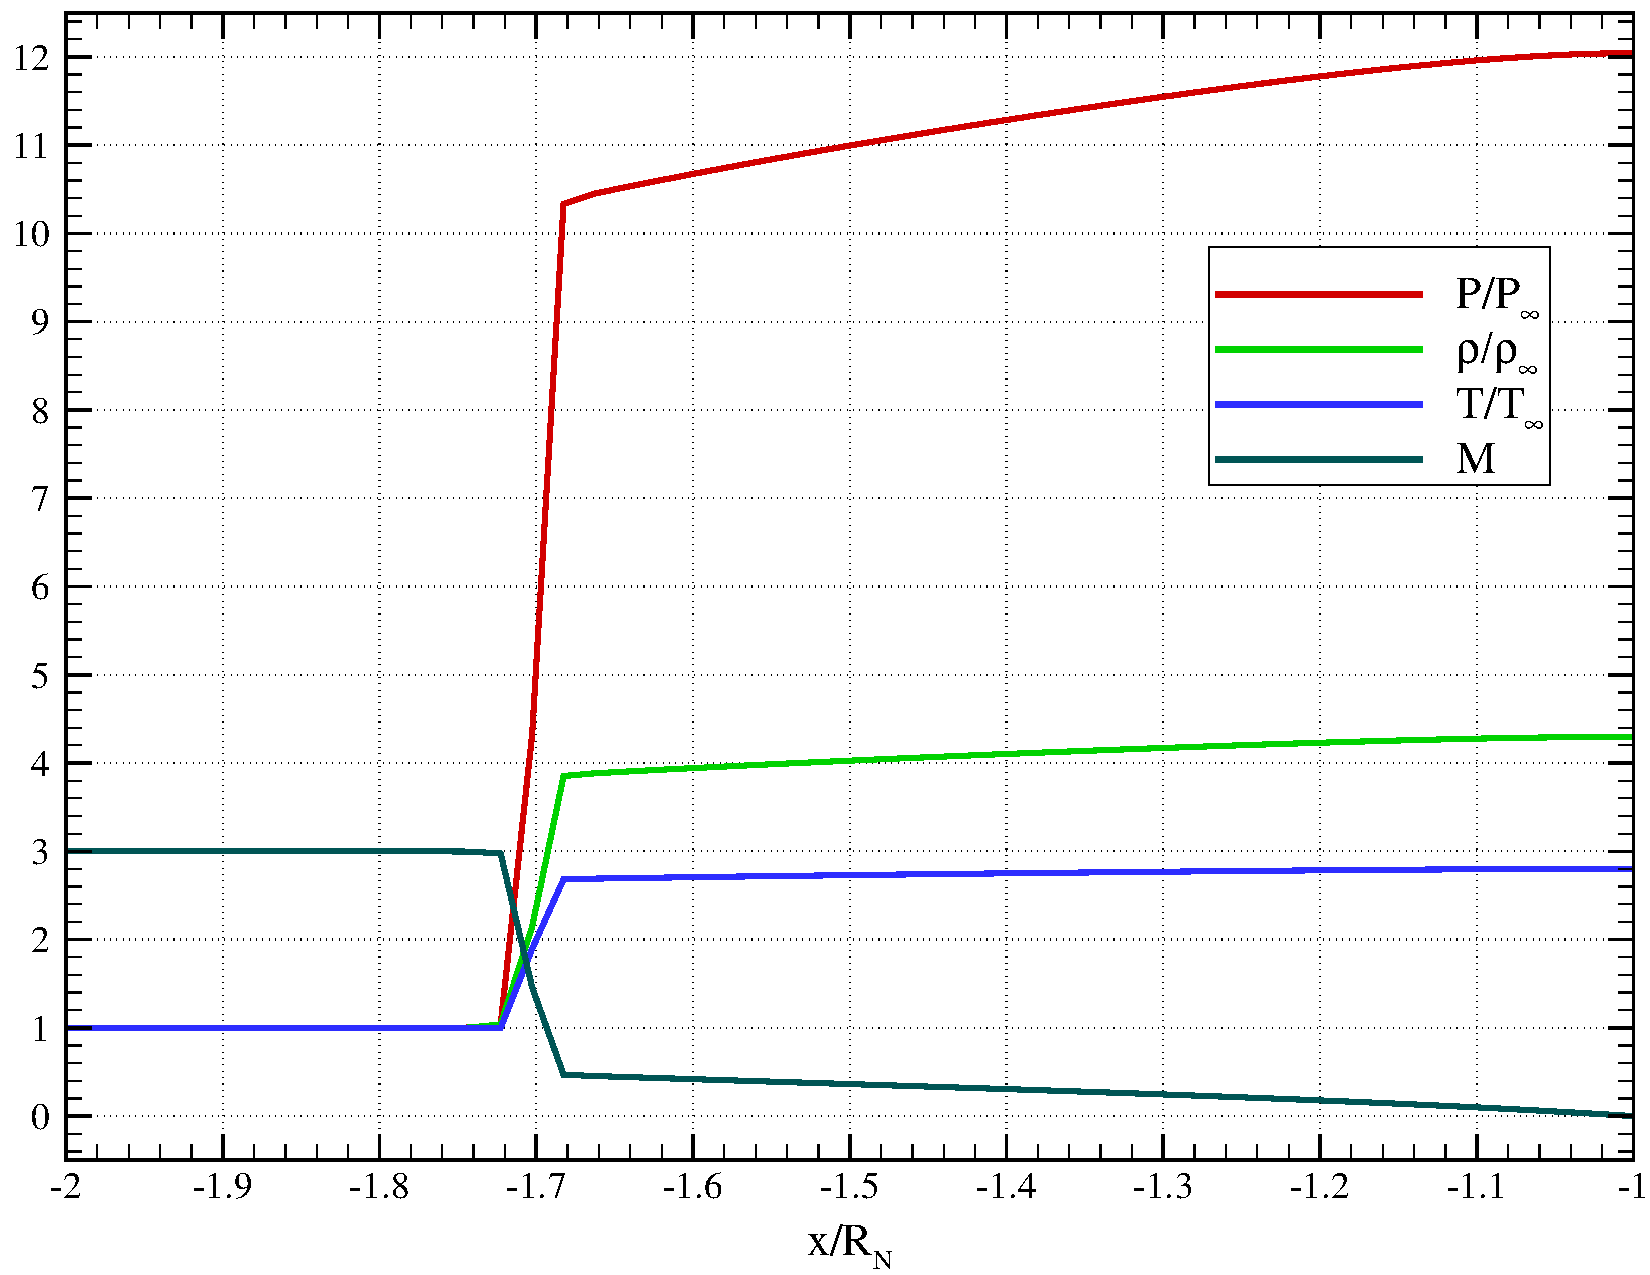
\includegraphics[width=\textwidth]{figures/mach3_cylinder/centerline} \\
    \caption{Stagnation line profile for Mach~3 flow over a cylinder\label{fig:cyl_stagline}}
  \end{center}
\end{figure}
It is apparent from the figure that the bow shock is located at approximately $0.7\,\text{R}_\text{N}$ upstream from the stagnation point, which agrees well with experimentally measured values~\cite{ambrosio_wortman}.  As expected, the pressure, density, and temperature all increase across the shock wave while the Mach number decreases.  The computed jumps are in excellent agreement with theoretical predictions as evident in Table~\ref{table:cyl_jumps}.
This indicates that the numerical scheme is properly reproducing the shock jump conditions, which is expected for any viable formulation based on the conservation form of the governing equations~\eqref{eq:pde_comp_mass}--\eqref{eq:pde_comp_energy}. Note that other formulations which are not based on the conservation form of the governing equations are possible and may provide simpler discretizations~\cite{pjcapon_dissertation}.  In general, however, these formulations \emph{will not} converge to a solution which satisfies the Rankine--Hugoniot equations.  Therefore, such schemes would not produce proper jump conditions for this case.
\begin{table}[hbtp]
  \begin{center}
    \caption{Computed and theoretical jump values for a Mach~3 normal shock.\label{table:cyl_jumps}}
    \vspace{1em}
    \begin{tabular}{l||ccc} \hline\hline
                                   & $P/P_\infty$ & $\rho/\rho_\infty$ & $T/T_\infty$ \\ \hline
      Theory~\cite{naca_1135} & 10.33 & 3.857 & 2.679 \\ 
      Computation             & 10.34 & 3.854 & 2.683 \\ \hline \hline
    \end{tabular}
  \end{center}
\end{table}

This example also serves as a good test case for the shock--capturing operator~$\delta$.  The stagnation line profiles depicted in Figure~\ref{fig:cyl_stagline} show that the shock is captured over 2--3 elements without spurious oscillations when the shock is essentially aligned with the grid.  This stagnation line will be revisited in Section~\ref{sec:comp_ns_cylinder_AMR} in the context of mesh convergence and adaptive mesh refinement.

\subsubsection{Convergence}
In order to better characterize both the transient and nonlinear discretization schemes described in Section~\ref{sec:comp_solution_methodology}, a series of numerical experiments were conducted which varied (1) the order of the time discretization and (2) the number of subiterations used to solve the discrete, nonlinear, implicit problem which results at each time step. For these higher fidelity numerical experiments a mesh of $n_\xi\times n_\eta=120\times 160$ elements was used. A discussion of mesh convergence will be presented following the algorithmic performance investigation.

\paragraph{Temporal Convergence to Steady-State}
\begin{figure}[hbtp]
  \begin{center}
    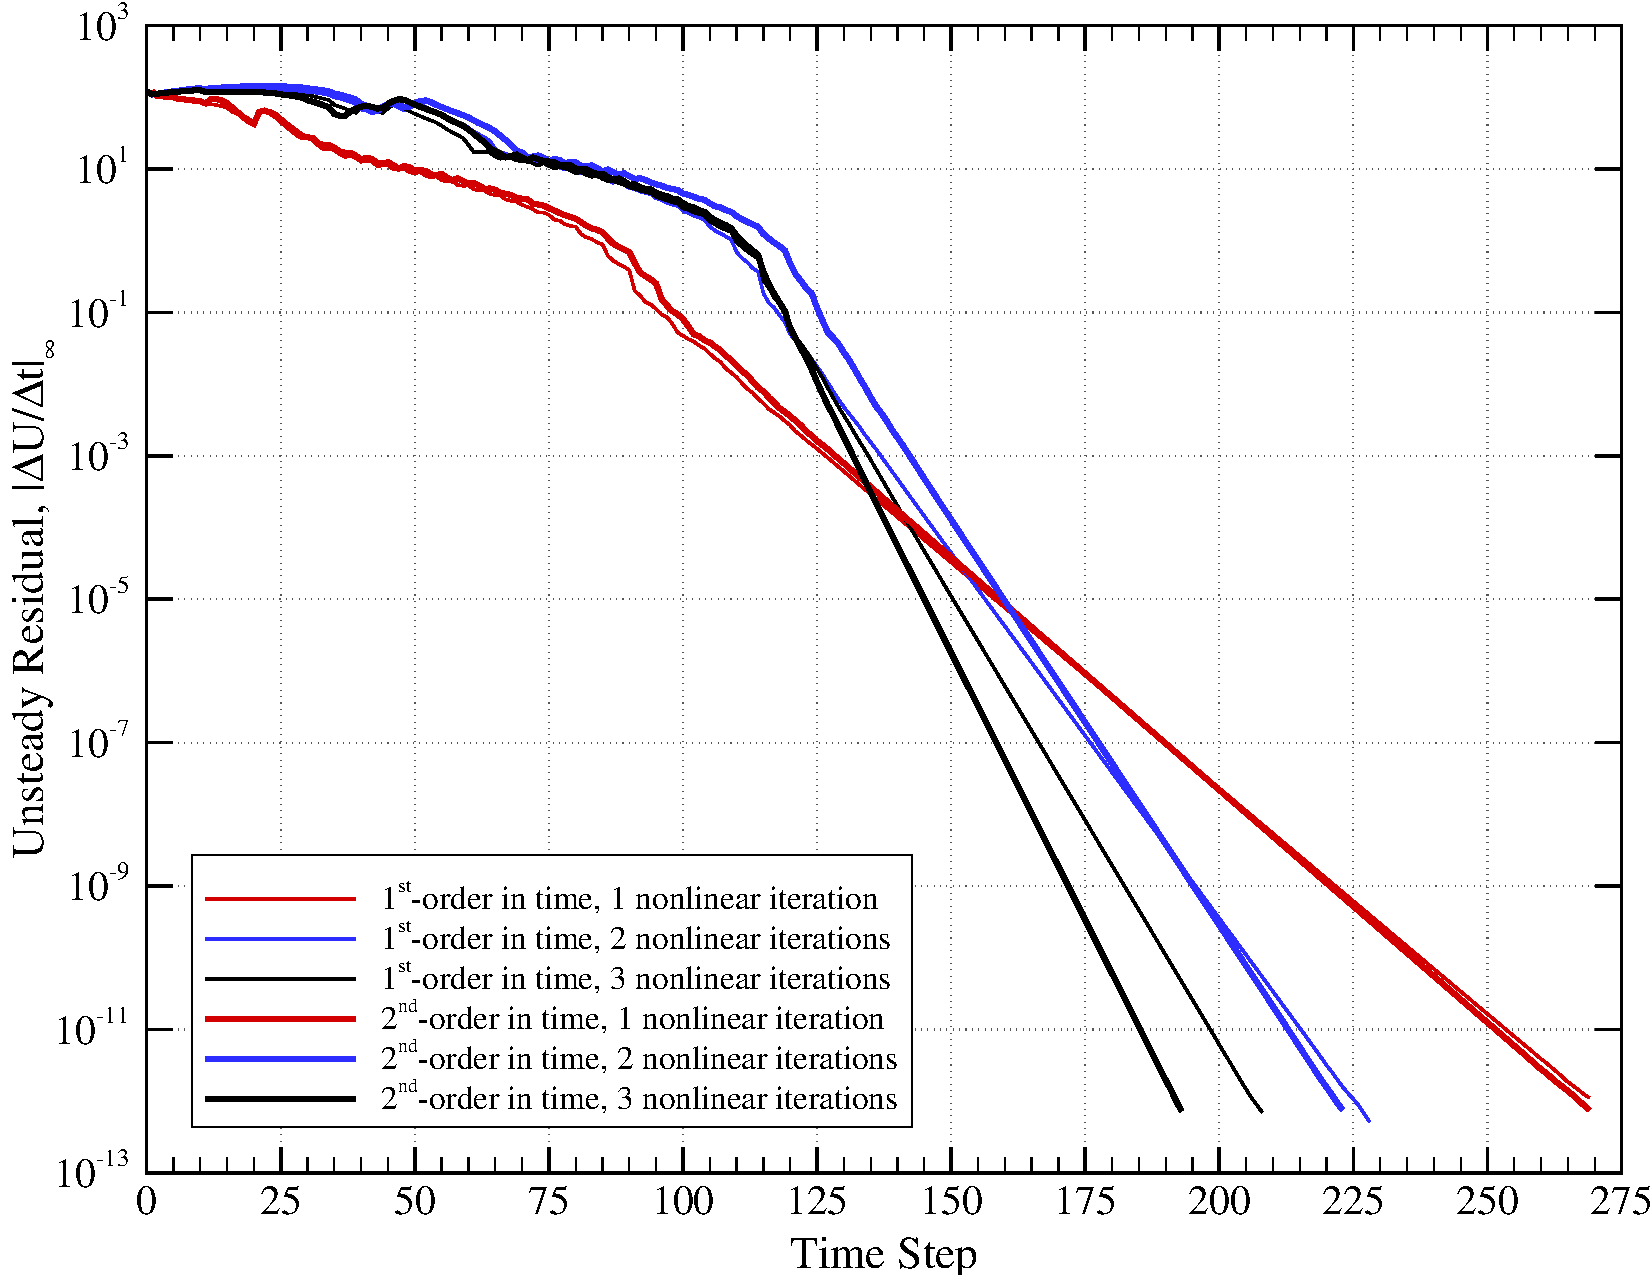
\includegraphics[width=\textwidth]{figures/mach3_cylinder/time_convergence}
    \caption{Time step convergence history for Mach~3 flow over a cylinder for a range of nonlinear solver subiterations and time discretizations.\label{fig:cyl_time_convergence}}
  \end{center}  
\end{figure}
%The case of inviscid supersonic flow over a blunt forebody considered in this section is expected to result in a steady flowfield for a given, steady freestream condition.
The absence of viscosity-induced separation, wake flow, and shock interaction produces a fairly simple, steady flowfield.  It is therefore expected that the numerical scheme will converge to a steady-state, which is assumed to be reached when the discrete unsteady residual, $\frac{\Delta \bv{U}}{\Delta t}$, falls below a user-specified tolerance  $\varepsilon_{ss}$ in the maximum norm.  That is, steady-state is assumed when
\begin{equation}
  \mathcal{R}_n \equiv \left\|\frac{\Delta \bv{U}_n}{\Delta t_n}\right\|_{\infty} < \varepsilon_{ss}
\end{equation}
where $\varepsilon_{ss}$ is the steady-state solution tolerance and was taken as $\varepsilon_{ss}=10^{-12}$.
The simulation begins with the domain initialized to freestream conditions everywhere and a user-specified initial time step $\Delta t_0$ is used to advance the solution, which was taken here as $2\times 10^{-3}$.  The time step is allowed to grow geometrically with the relative change in the unsteady residual measured over $k$ time steps.  Explicitly, 
\begin{align}
  \Delta \bar{t}_{n+1} &= \Delta t_{n-k} \left[\frac{\mathcal{R}_{n-k}}{\mathcal{R}_{n}}\right]^r \label{geometric_timestep_growth} \\ \vspace{1em}
                 & \nonumber \\
  \Delta t_{n+1} &= \min\left(\Delta \bar{t}_{n+1},\Delta t_{\text{max}}\right) \label{dt_limiting}
\end{align}
where $r$ is the geometric time step growth rate, which was fixed at 1.2 in this case.  The time step size is updated every $k=5$ time steps and the maximum allowable time step $\Delta t_{\text{max}}=1$ corresponds to the amount of time required for a fictitious point in the freestream to be convected one cylinder diameter.

One immediate observation from the numerical experiments is that the 1\textsuperscript{st}- and 2\textsuperscript{nd}-order time discretizations exhibit similar transient convergence behavior. The convergence history exhibits two distinct phases: (1) the pre-asymptotic phase in which the bow shock develops and travels upstream to its steady location and (2) the asymptotic phase where large-scale changes in the flowfield have subsided and the remaining transient behavior is damped out.

In the pre-asymptotic phase the time discretization order of accuracy has little influence on the convergence rate.  This is consistent with the observation that, during this highly nonlinear process, the time step size must be limited to achieve convergence of the nonlinear subproblem. In the asymptotic phase the convergence rate of the two schemes is again comparable. Since the only added cost associated with the 2\textsuperscript{nd}-order scheme is the storage of an additional solution vector, there seems to be no compelling motivation to use the 1\textsuperscript{st}-order scheme.  Additionally, using the 2\textsuperscript{nd}-order scheme will more accurately capture any unsteady flow phenomena which might occur for a given configuration.

It is interesting that the current finite element scheme does not exhibit the nonlinear residual convergence stagnation noted by Catabriga and Coutinho when using a very similar SUPG finite element scheme for the conservation variables~\cite{catabriga_coutinho_SUPG_convergence}.  This difference must be due to either (i) the inviscid flux treatment used in the present scheme or (ii) the integration by parts performed on the inviscid flux terms since the remainder of the discretized weak form is identical.

\paragraph{Nonlinear Solver Accuracy}
\begin{figure}[hbtp]
  \begin{center}
    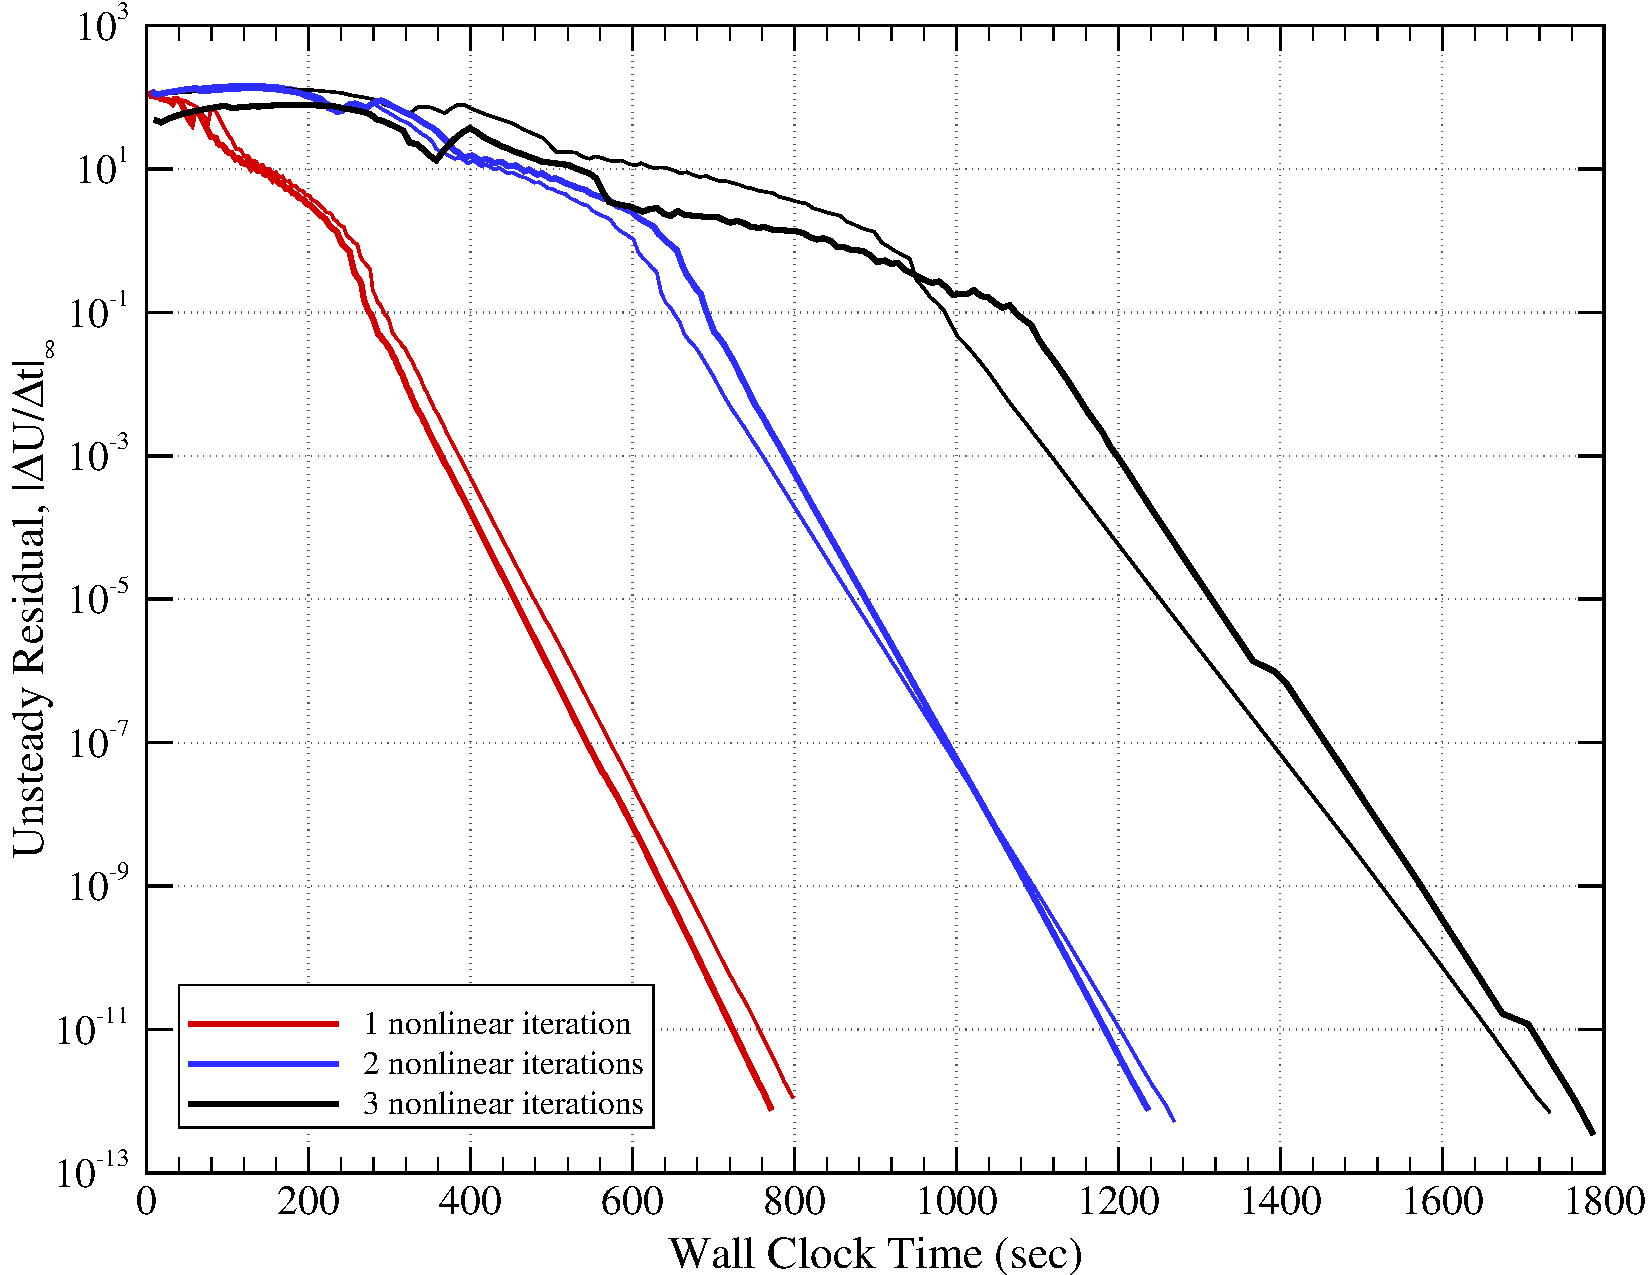
\includegraphics[width=\textwidth]{figures/mach3_cylinder/walltime_convergence}
    \caption{Wall clock convergence history for Mach~3 flow over a cylinder for a range of nonlinear solver subiterations and time discretizations.\label{fig:cyl_wallclock_convergence}}
  \end{center}  
\end{figure}
A first glance at Figure~\ref{fig:cyl_time_convergence} might suggest that the algorithm performs better when specifying a larger number of nonlinear iterations per time step. In this case the figure is misleading because, in the current implementation, the computational cost of each time step is proportional to the number of nonlinear iterations used. 
Figure~\ref{fig:cyl_wallclock_convergence} shows the unsteady residual versus wall-clock time for the cases previously mentioned.  Note that the trend observed in the previous figure is now reversed.  The wall clock time is seen to increase directly with the number of nonlinear iterates.  Thus, even though the case of three nonlinear iterations per time step converges in the shortest number of physical time steps it clearly is the most expensive in terms of wall clock time.

This study supports the common practice of performing only one nonlinear solution iterate per time step when considering steady flows, therefore future examples which consider stationary flows will only perform one nonlinear iteration per time step.  It must be emphasized that this truncated nonlinear problem is essentially a pseudo-time continuation procedure and, that for cases where transient behavior is of interest, the nonlinear problem at each time step must be solved to an accuracy commensurate with other aspects of the algorithm.

While the wall clock time required increases with the number of nonlinear solver subiterations, it is interesting that it does not increase linearly.  This is because at each subsequent nonlinear iteration the underlying linear system is solved with an iterative Krylov subspace method which benefits from the accuracy of the initial iterate.  The linear solver for each subsequent nonlinear iteration in general converges more rapidly than the one before, hence the overall scaling is not linear with the number of nonlinear subiterations.

Note that in this work the preconditioning matrix used in the linear solver is assembled and factored for each linear solve.  Follow-on work could consider the performance trade-off between recomputing the preconditioning matrix versus fixing the preconditioner for some number of iterations and accepting a less accurate approximate inverse matrix. Similar techniques were investigated by Barth~\cite{barth_dissertation} for incompressible non-Newtonian fluids and show promise for reducing the computational effort required per time step.

\paragraph{Mesh Convergence}
A series of nested meshes consisting of $n_\xi\times n_\eta=60\times 80$, $120\times 160$, and $240\times 320$ elements was used, as well as an adaptive mesh.Typical results for the stagnation line density profile are shown in Figure~\ref{fig:cyl_meshconv}.
\begin{figure}[hbtp]
  \begin{center}
    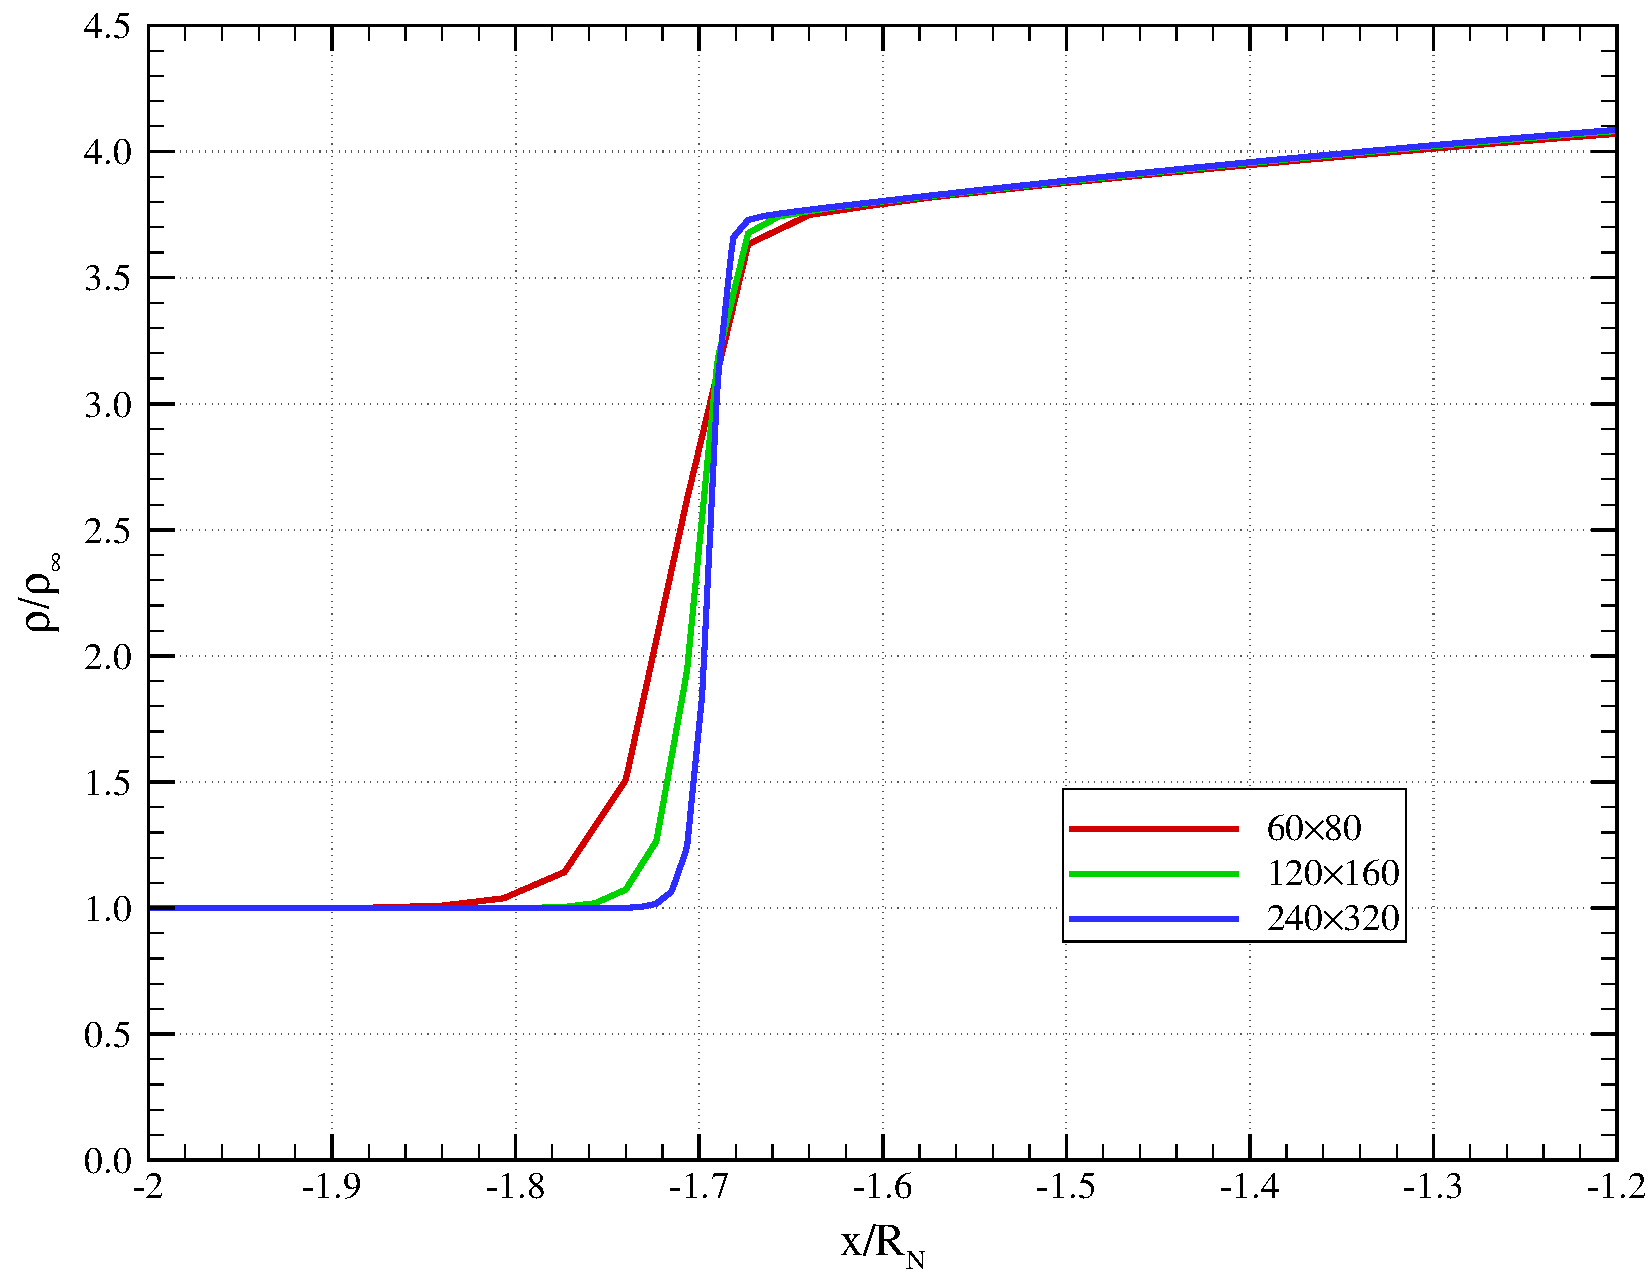
\includegraphics[width=\textwidth]{figures/mach3_cylinder/rho_mesh_convergence}
    \caption{Stagnation line density profile for Mach~3 flow over a cylinder at a series of mesh resolutions.\label{fig:cyl_meshconv}}
  \end{center}
\end{figure}
  The figure shows the density jump which occurs across the bow shock along the stagnation line.  For the series of nested meshes both the location and strength (indicated by the density jump across the shock) of the bow shock is consistent for all three simulations.  Interestingly, the location of the trailing edge of the shock wave is more consistent across the series of meshes than the leading edge of the shock.  
\begin{figure}[hbtp]
  \begin{center}
    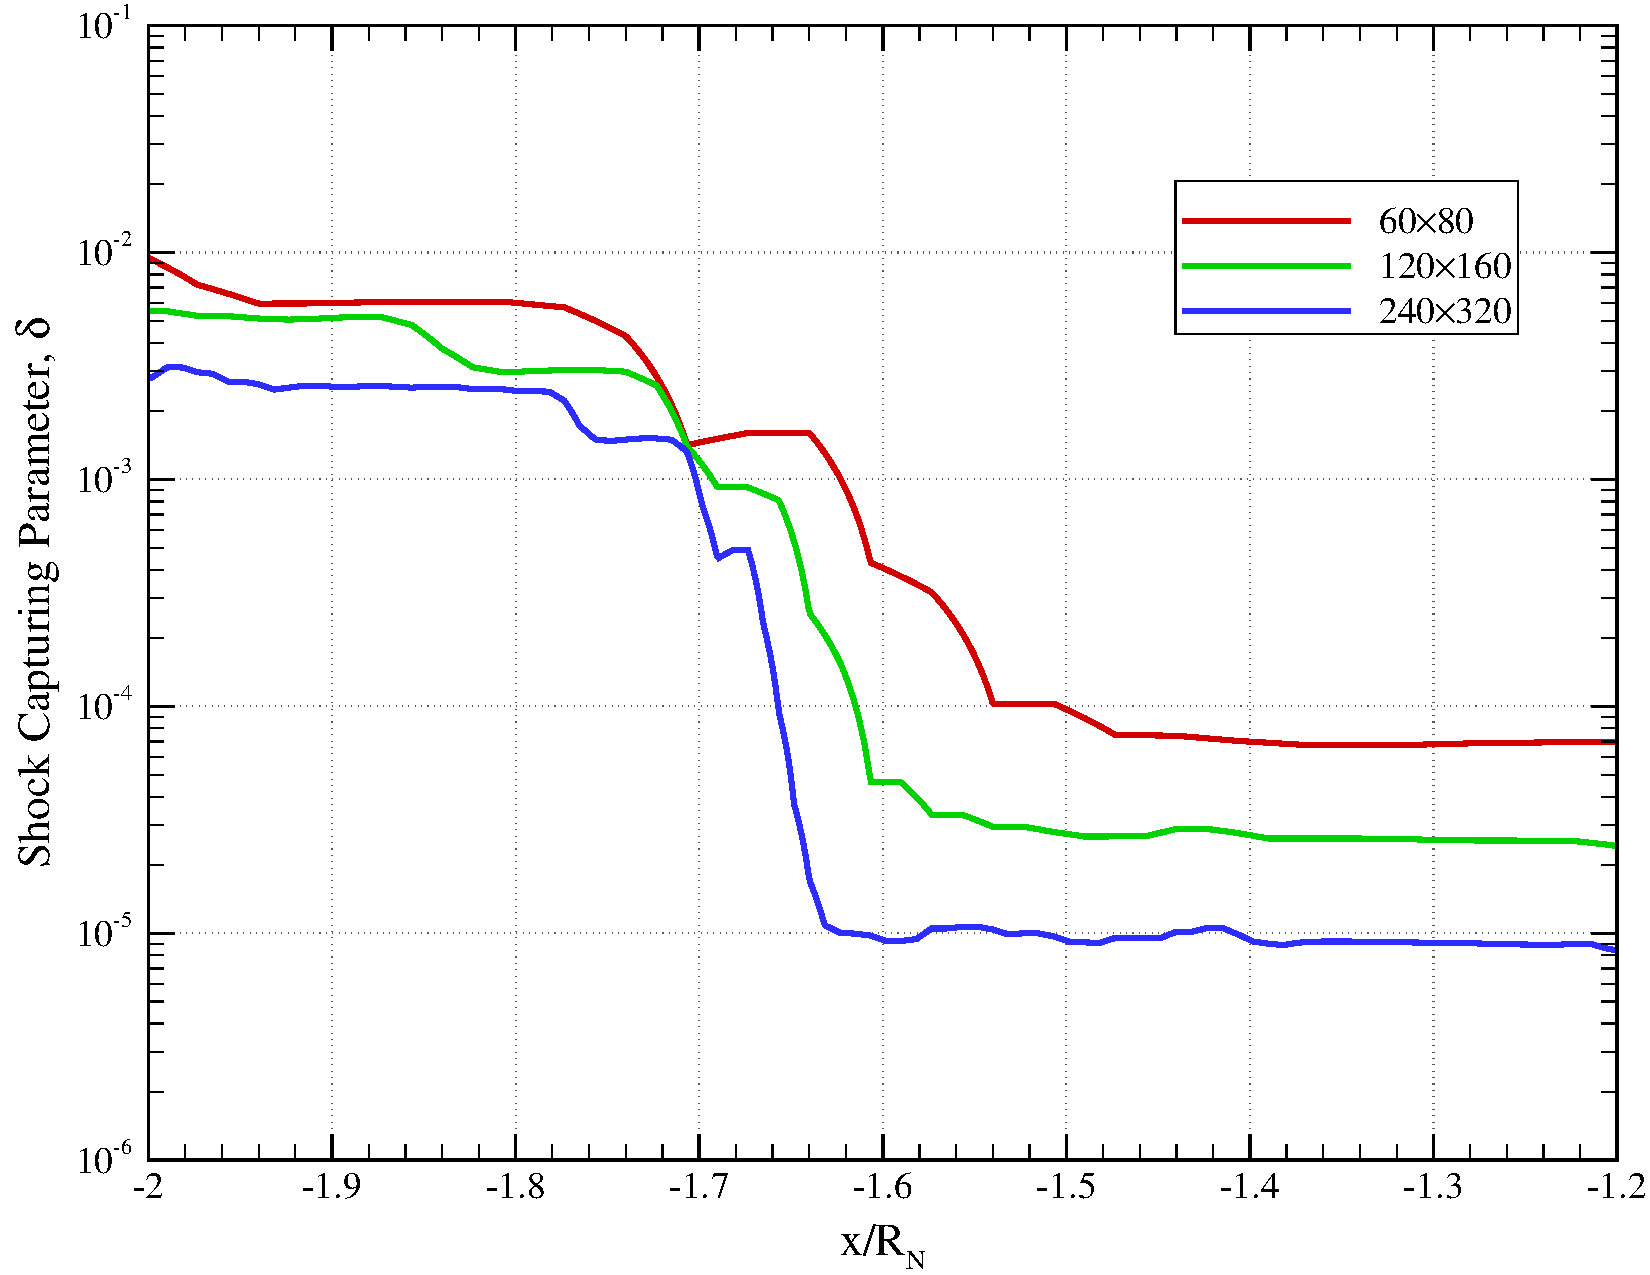
\includegraphics[width=\textwidth]{figures/mach3_cylinder/delta_mesh_convergence}
    \caption{Stagnation line shock capturing parameter profile for Mach~3 flow over a cylinder at a series of mesh resolutions.\label{fig:cyl_deltaconv}}
  \end{center}
\end{figure}

Figure~\ref{fig:cyl_deltaconv} shows the shock capturing parameter, $\delta$, along the stagnation line for the three nested meshes.  Interestingly, in all cases the shock capturing parameter peaks \emph{upstream} of the bow shock in the uniform freestream.  Upon returning to Equation~\eqref{eq:shock_capturing_parameter} it is clear that in the uniform freestream the term behaves as $\mathcal{O}(0/0)$, and the relatively large magnitude of the parameter is a numerical artifact.  Since the flow is uniform in this region the artificial diffusion term weighted by $\delta$ is inconsequential, so this behavior, albeit unsettling, does not adversely affect the quality of the solution.

The parameter decreases nearly monotonically through the bow shock and reaches a steady, low value in the post-shock stagnation region.  The post-shock value of the shock capturing parameter decreases from approximately $10^{-4}$ to $10^{-5}$ with two levels of uniform mesh refinement.  Since this corresponds to a factor of four reduction in the mesh spacing $h$, for this case $\delta$ appears to decrease superlinearly with $h$.  For this case $\delta\propto h^{1.5}$.

\subsubsection{Adaptive Mesh Refinement\label{sec:comp_ns_cylinder_AMR}}
The primary feature of this flow is the bow shock created by the cylinder.  This feature is highly localized, and therefore could be captured effectively with an adaptive technique.  To assess the viability of the adaptive approach for this stationary inviscid flow the simulation was repeated on the coarsest background mesh $(60\times80)$.  The gradient indicator of Equation~\eqref{eqn:flux_indicator} was used to select which elements would be refined.  

The simulation was initialized as before with the freestream conditions specified everywhere in the domain.  The solution was then marched in time on the coarse mesh until the bow shock reached its  steady location.  This allowed the majority of the transient startup phase to be performed at little cost on the coarse mesh.  Once the solution on this coarse mesh became steady, the adaptive mesh refinement process was initiated.  The maximum level of refinement was restricted to four, which would correspond in the fine mesh regions to a uniform mesh of $480 \times 640$ elements.  The resulting mesh, colored by density, is shown in Figure~\ref{fig:cyl_amr}.
\begin{figure}[hbtp]
  \begin{center}
    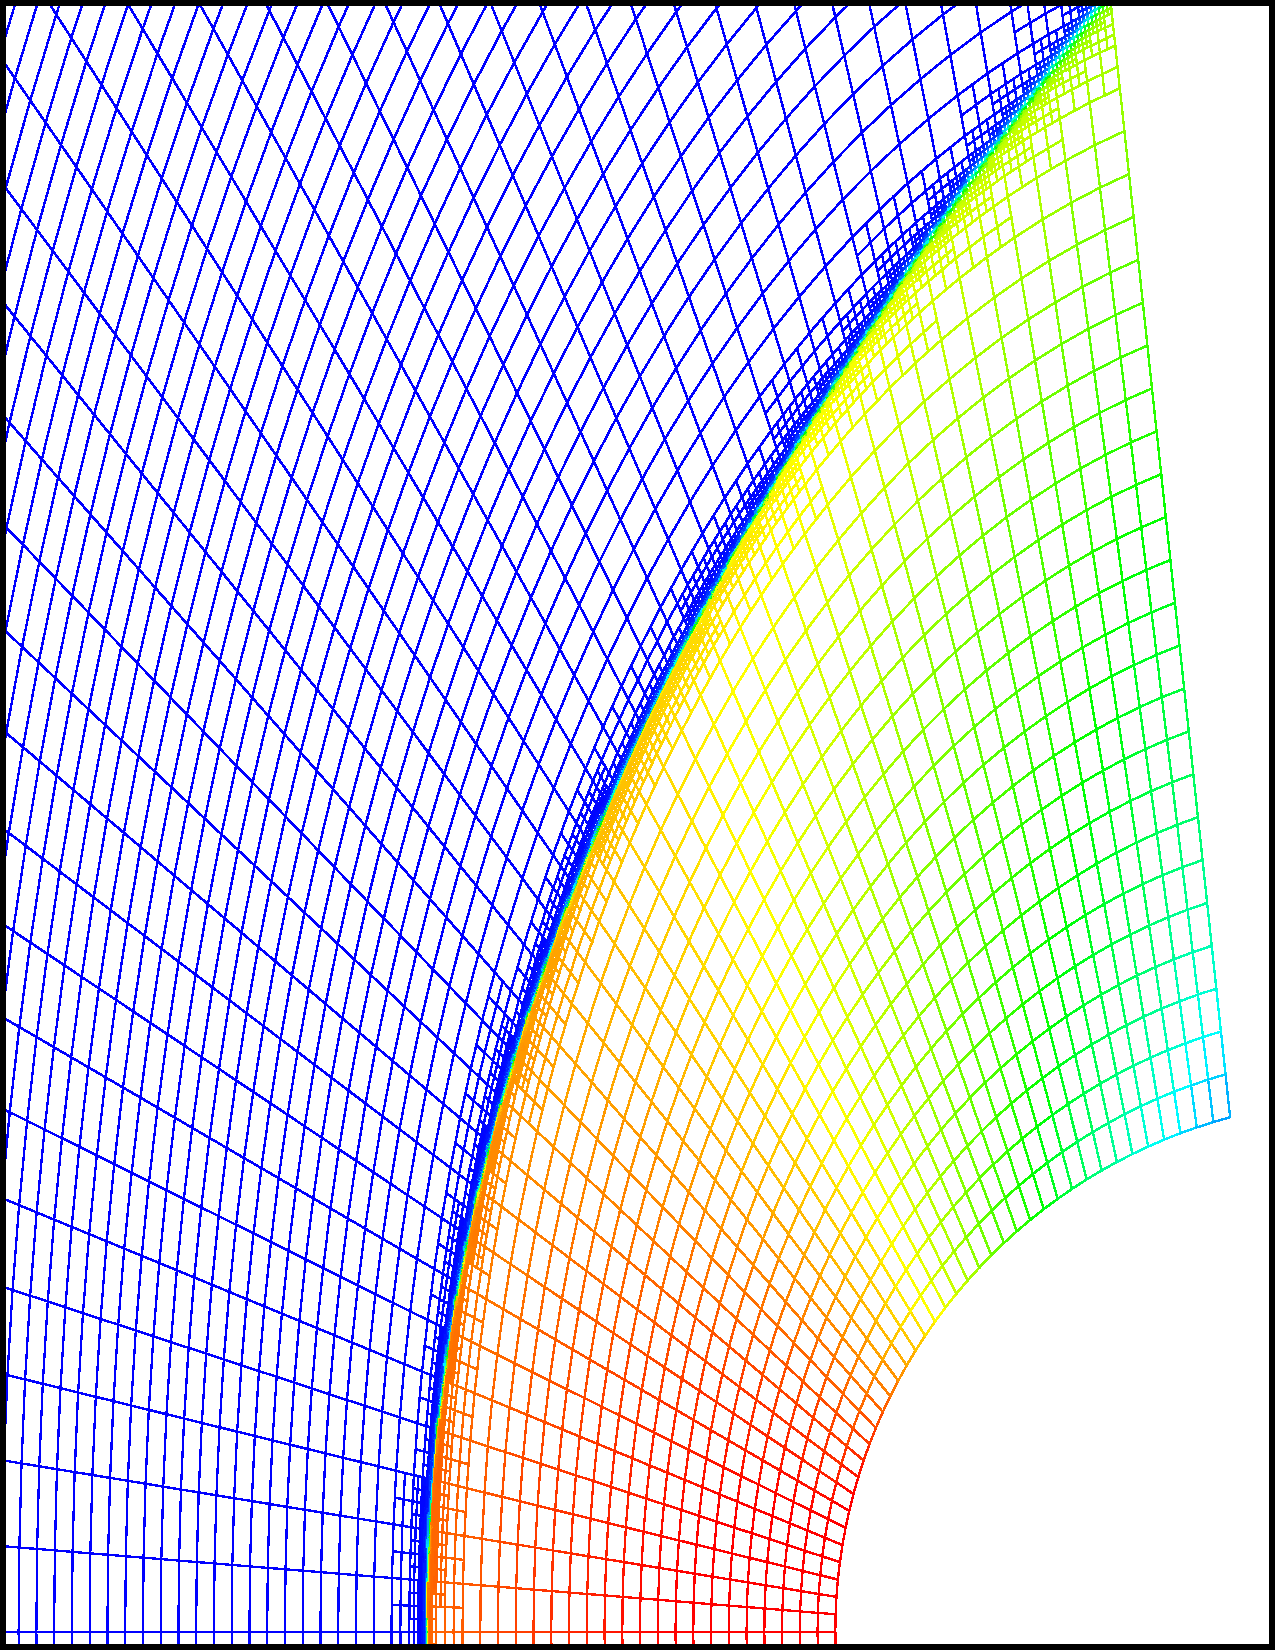
\includegraphics[height=.85\textheight]{figures/mach3_cylinder/rho_amr_mesh}
    \caption[Adapted mesh capturing the bow shock for Mach~3 flow over a cylinder.]{Adapted mesh capturing the bow shock for Mach~3 flow over a cylinder.  The mesh is colored by the density.\label{fig:cyl_amr}}
  \end{center}
\end{figure}

The resulting computational mesh contains 26,076 cells and 27,434 nodes for a total of 109,736 degrees of freedom.  To achieve the same local mesh resolution in the vicinity of the shock wave using a $480 \times 640$ mesh would require 307,200 cells (12 times as many cells as in the adapted mesh).  Of course, a non-adapted mesh of this resolution would clearly afford a higher-accuracy global solution, so the comparison is not entirely fair.  Still, the savings afforded by local mesh refinement are significant, especially when considering that the smaller, adapted mesh may be run quickly on a modest desktop machine.

It was mentioned previously that the shock-capturing scheme used in this work smears the shock wave across 2-3 elements when the shock is aligned with the mesh.  The scheme is more diffusive when the shock and mesh are not aligned, capturing the feature smoothly across approximately four elements.  The adaptive mesh refinement process does remarkably well at refining the mesh in this region to increase the resolution of the captured shock even though the background mesh is not aligned with the feature.

A common practice in finite volume simulations of hypersonic flows is to ``tailor'' the outer boundary of the mesh to the location of a shock wave.  In this process the location of the outer boundary is moved to just upstream of the shock and its orientation is changed such that the shock is parallel to element interfaces.  This necessarily introduces some distortion into the mesh which can degrade overall solution accuracy.  The present adaptive procedure provides an alternate approach for accurately capturing a strong shock wave which preserves the qualities of the original mesh.

As noted in Section~\ref{sect:comp_sc}, the additional shock-capturing parameter used to regularize the problem renders the scheme locally 1\textsuperscript{st}-order accurate in the vicinity of shock waves.  The only viable approach for increasing the solution accuracy in this case is to reduce the local mesh size substantially.  The adaptive refinement procedure does exactly that.  By rapidly decreasing the mesh size in the vicinity of a shock wave the overall accuracy of the solution is increased.

The stagnation line density profile presented earlier is revisited with the adaptive results in Figure~\ref{fig:cyl_amr_rho_stagline}.
\begin{figure}[hbtp]
  \begin{center}
    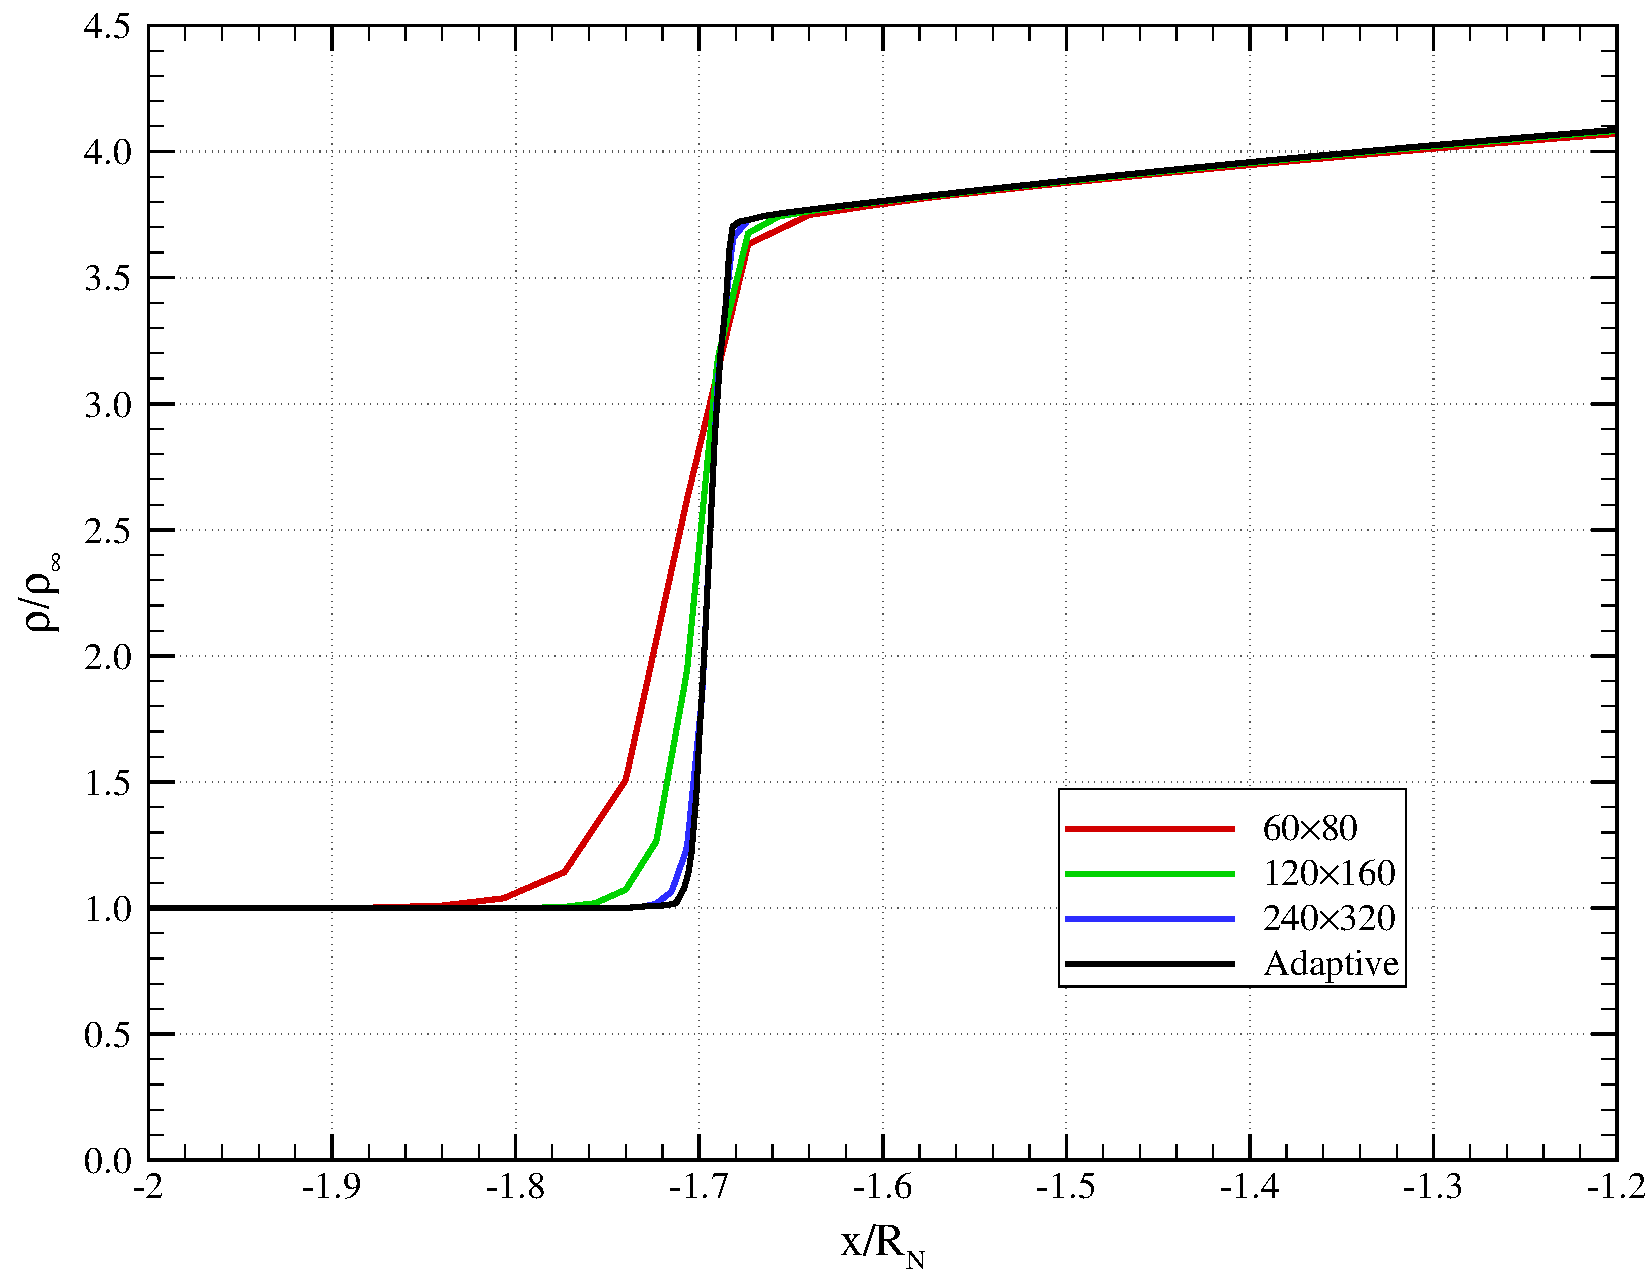
\includegraphics[width=\textwidth]{figures/mach3_cylinder/rho_amr_mesh_convergence}
    \caption{Stagnation line density profile for uniform and adapted meshes capturing the bow shock for Mach~3 flow over a cylinder.\label{fig:cyl_amr_rho_stagline}}
  \end{center}
\end{figure}
The adaptive result continues the trend that was observed previously, namely that the shock foot moves progressively downstream as the mesh is refined.  The post-shock location is essentially constant for all meshes considered.  The adapted mesh, with its finer spacing in the shock region, provides the sharpest shock wave.




%%%%%%%%%%%%%%%%%%%%%%%%%%%%%%%%%%%%%%%%%%%%%%%%%%%%%%%%%%%%%%%%%%%%%%%%%%%%%%%
%\clearpage
\subsection{Hypersonic Flow over a Compression Ramp\label{sec:comp_ns_ramp}}
This case considers laminar hypersonic flow over a 15$^\circ$ compression ramp.  The freestream Mach number is 11.68, temperature is \unit[64.6]{K}, and unit Reynolds number is \unitfrac[558,000]{1}{m}. Figure~\ref{fig:holden_shock_ramp_schematic} illustrates the ramp geometry and boundary conditions.  The Reynolds number based on the flat plate length is Re$_L=$246,636~\cite{holden_laminar_interaction,holden_interaction_review,hypersonic_benchmarks}.
% Holden compression ramp - schematic
\begin{figure}[hbtp]
  \begin{center}
    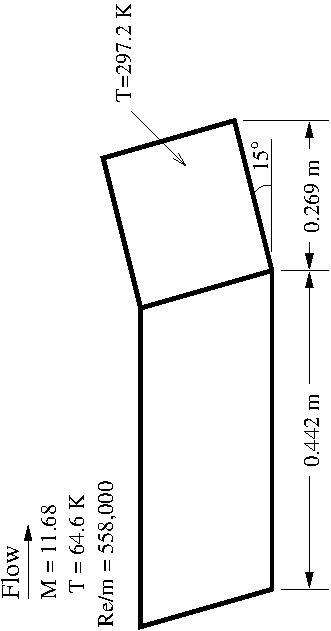
\includegraphics[height=6in,angle=270]{figures/holden_ramp/ramp}
    \caption{Illustration of geometry and boundary conditions for hypersonic shock ramp problem}
    \label{fig:holden_shock_ramp_schematic}
    \end{center}
\end{figure}
The freestream conditions for this case are explicitly listed in Table~\ref{table:compression-ramp-freestream-parameters}.
% Holden compression ramp - freestream parameters
\begin{table}[hbtp]
  \begin{center}
    \caption[Freestream parameters for hypersonic compression ramp.]{Freestream parameters for hypersonic compression ramp~\cite{holden_laminar_interaction,hypersonic_benchmarks}.\label{table:compression-ramp-freestream-parameters}}
    \vspace{1em}
    \begin{tabular}{cccc} \hline \hline
      M$_\infty$ & Re$_L$  & T$_\infty$ & T$_w$     \\
      11.68      & 246,636 & \unit[64.6]{K}   & \unit[297.2]{K} \\ \hline
    \end{tabular}
  \end{center}
\end{table}

\subsubsection{Motivation}
Supersonic flow over a compression ramp is of interest in aerodynamic applications because it is analogous to a control surface deflecting into a supersonic flow.  For this case a weak shock will develop at the leading edge of the plate due to displacement thickness effects from the viscous boundary layer.   The boundary layer thickness will grow relatively quickly down the plate length due to the high edge Mach number.  The compression ramp will produce an additional weak shock which is required to deflect the incoming supersonic flow.  This weak shock causes a pressure increase on the compression ramp surface which can feed upstream in the subsonic portion of the boundary layer.  This adverse pressure gradient, in turn, will affect the laminar boundary layer itself and can induce separation.  For the case of control surface deflection the resulting pressure distribution on the compression ramp is of interest because it will dictate the performance of the control surface itself.  Additionally, the heat transfer in this interaction region is also of interest because localized peaks can occur due to the laminar shock/boundary layer interaction, and these effects must be accounted for in the control surface design.


\subsubsection{Computational Mesh}
A single structured grid was used to discretize the domain and is shown in Figure~\ref{fig:ramp_mesh}.
\begin{figure}[hbtp]
  \begin{center}
    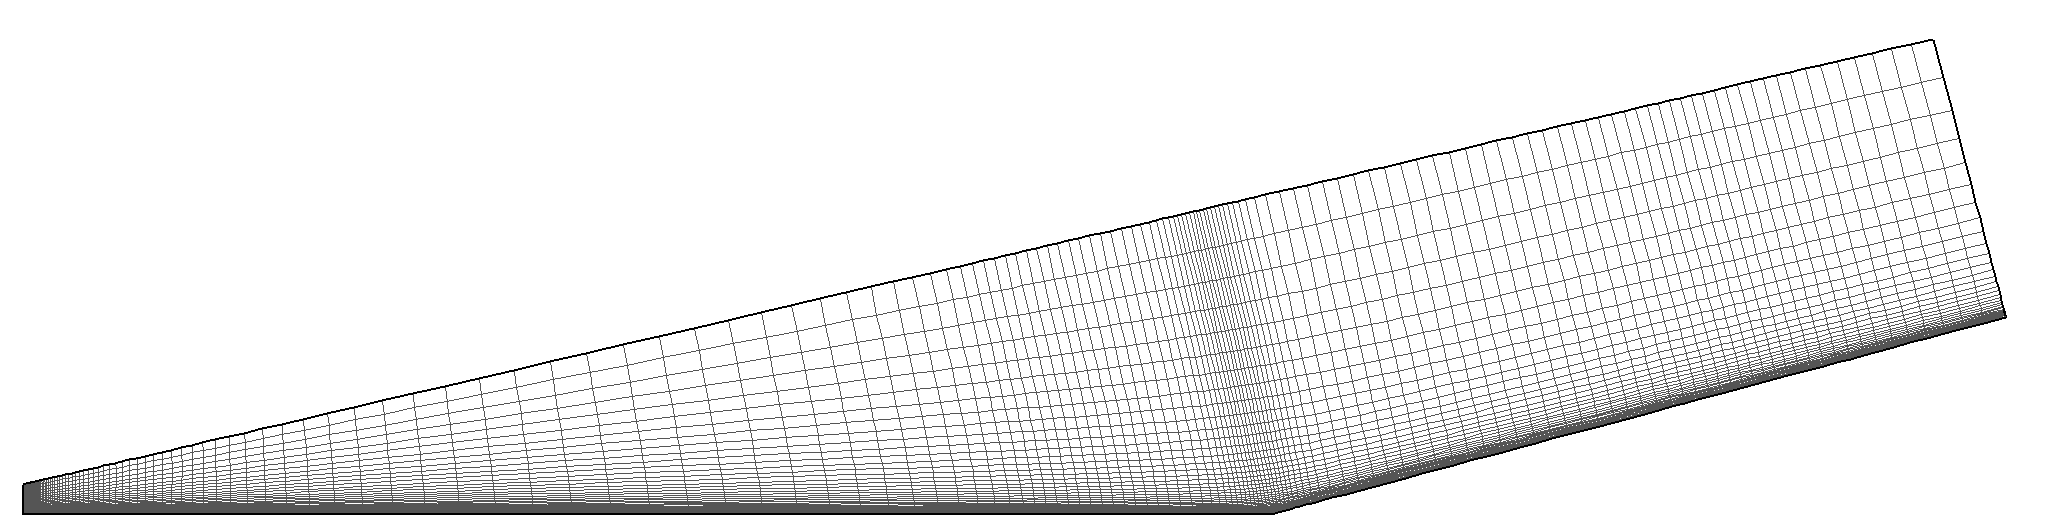
\includegraphics[width=\textwidth]{figures/holden_ramp/grid}
    \caption[Baseline computational mesh used for hypersonic flow over a compression ramp.]{Baseline computational mesh used for hypersonic flow over a compression ramp. (Every-other point is shown)\label{fig:ramp_mesh}}
  \end{center}
\end{figure}
The outer boundary of the grid was created with a straight segment from the leading edge of the plate to the outflow boundary.  The height of the outflow boundary was chosen such that the weak shock and subsequent Mach wave produced by the upstream portion would be fully contained within the flow domain. The left and upper boundaries are specified as freestream with essential boundary conditions.  The plate itself is modeled as an isothermal no-slip wall.  While not visible in the image, there is a very small region upstream of the plate leading edge which is modeled with a symmetry boundary condition.  Thus, there is a slip/stick boundary condition on the velocity at the leading edge of the plate.  The baseline non-adapted mesh used in the simulation contains 46,680 quadrilateral elements with 47,190 nodes, yielding a discrete problem with 188,760 degrees of freedom.  The mesh was partitioned into 6 subdomains and the simulation was run in parallel on a group of desktop-class machines. The partitioned mesh is shown in Figure~\ref{fig:ramp_partitioned}. Note that due to the fine streamwise and normal mesh resolution used at the leading edge of the plate one of the subdomains is so physically small as to be barely visible in the Figure, although each subdomain contains roughly the same number of elements.  
\begin{figure}[hbtp]
  \begin{center}
    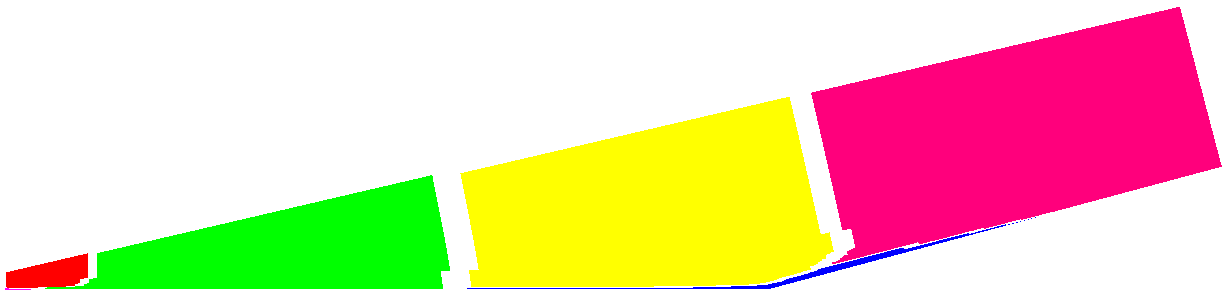
\includegraphics[width=\textwidth]{figures/holden_ramp/partitioned}
    \caption{Partitioned mesh  for hypersonic flow over a compression ramp.\label{fig:ramp_partitioned}}
  \end{center}
\end{figure}



\subsubsection{Results}
Figure~\ref{fig:holden_shock_ramp_global} depicts the global flowfield for this case.  The adverse pressure gradient induced by the compression ramp is evident in Figure~\ref{fig:holden_shock_ramp_P_global}.  This pressure gradient causes the boundary layer to separate upstream of the compression ramp.  The recirculation region is shown in detail in Figure~\ref{fig:holden_shock_ramp_recirculation}.
% Holden compression ramp 
\begin{figure}[hbtp]
  \begin{center}
    \subfigure[Mach Contours \label{fig:holden_shock_ramp_Mach_global}    ]{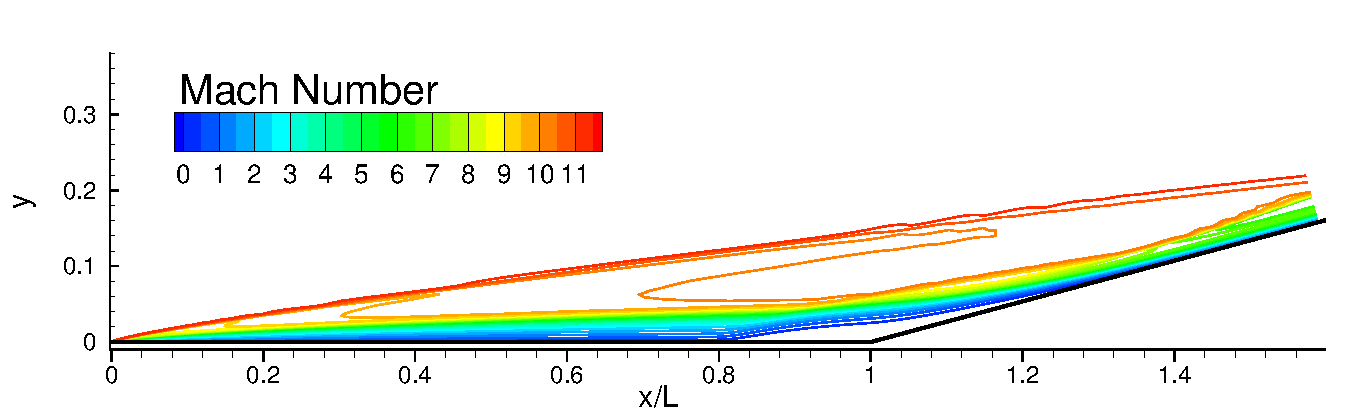
\includegraphics[width=\textwidth]{figures/holden_ramp/Mach}} \\
    \subfigure[Temperature Contours \label{fig:holden_shock_ramp_T_global}]{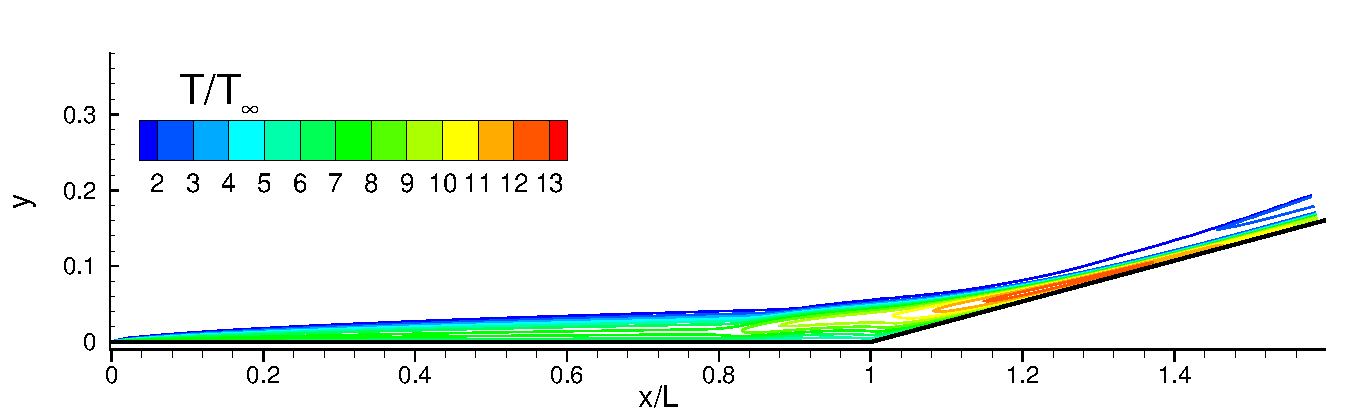
\includegraphics[width=\textwidth]{figures/holden_ramp/T}} \\
    \subfigure[Pressure Contours \label{fig:holden_shock_ramp_P_global}   ]{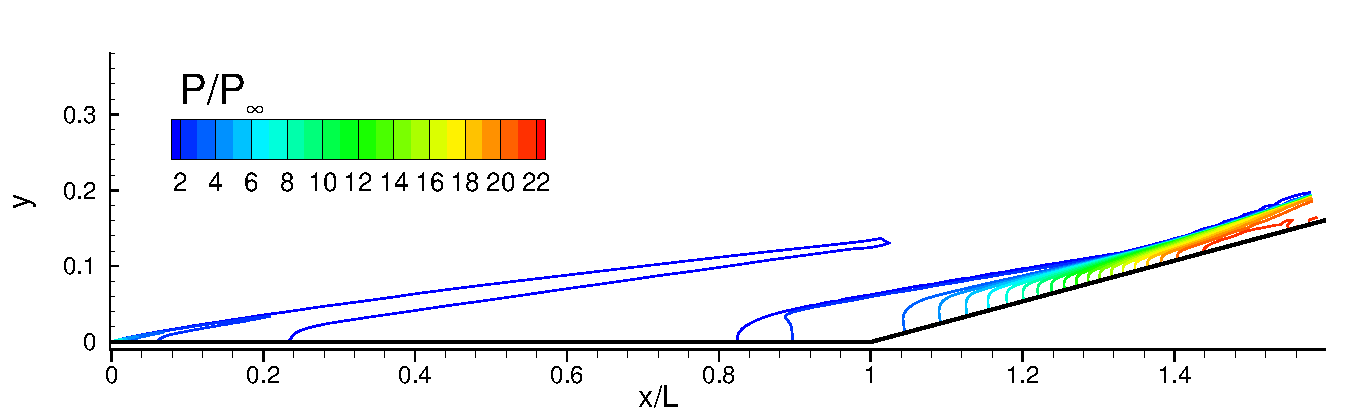
\includegraphics[width=\textwidth]{figures/holden_ramp/P}}
    \caption{Illustration of flowfield for hypersonic shock ramp problem\label{fig:holden_shock_ramp_global}}
  \end{center}
\end{figure}

% Holden compression ramp - recirculation region
\begin{figure}[hbtp]
  \begin{center}
    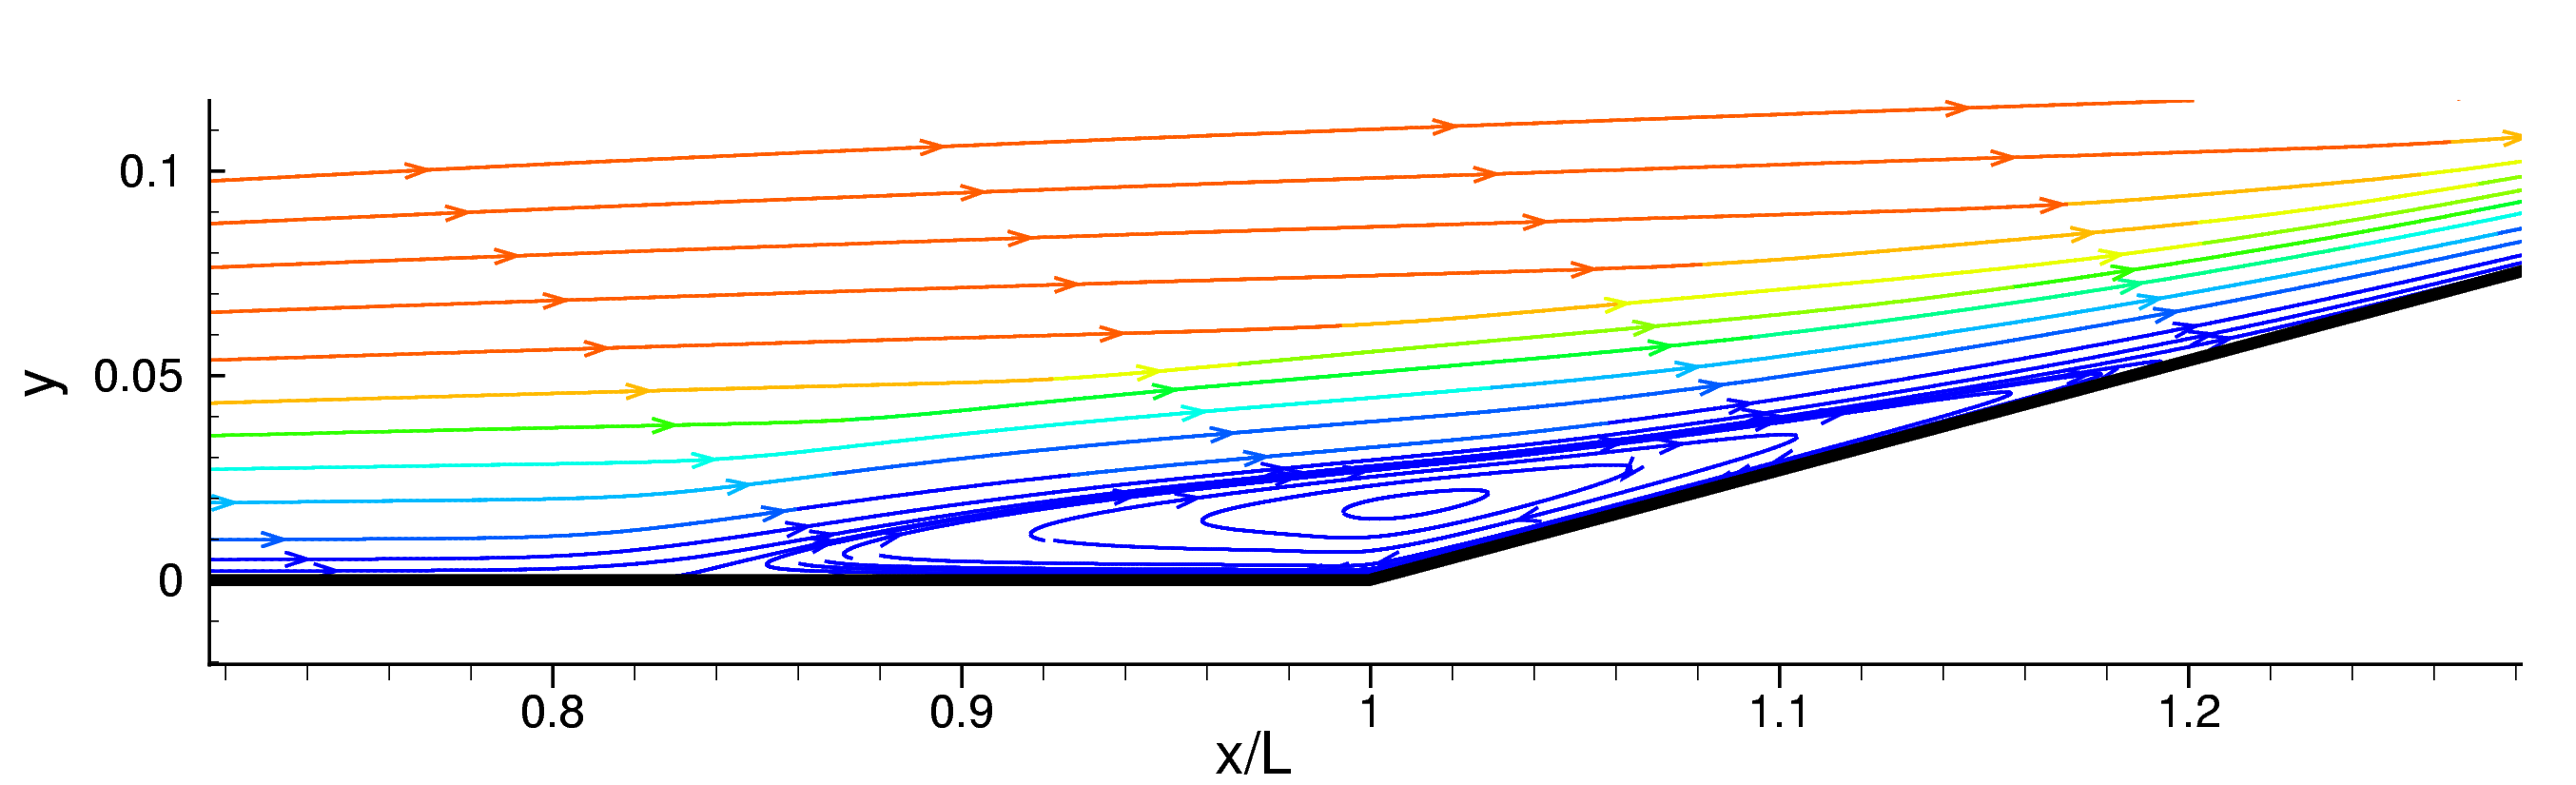
\includegraphics[width=\textwidth]{figures/holden_ramp/recirculation}
    \caption{Compression ramp recirculation region\label{fig:holden_shock_ramp_recirculation}}
  \end{center}
\end{figure}

Figures~\ref{fig:holden_shock_ramp_exp_cf} and~\ref{fig:holden_shock_ramp_exp_st} compares the computed skin friction coefficient and Stanton number distribution with measurements made by Holden~\cite{holden_laminar_interaction}.  The experimental data were obtained in the Calspan 48-inch shock tunnel.  The test article was instrumented with thin-film heat transfer gages, pressure transducers, and skin friction transducers along the centerline.  A range of plate widths were tested to ensure that the centerline data were not adversely affected by three-dimensional expansion effects~\cite{holden_laminar_interaction}.

%\clearpage
% Holden compression ramp - skin friction
\begin{figure}[hbtp]
  \begin{center}
    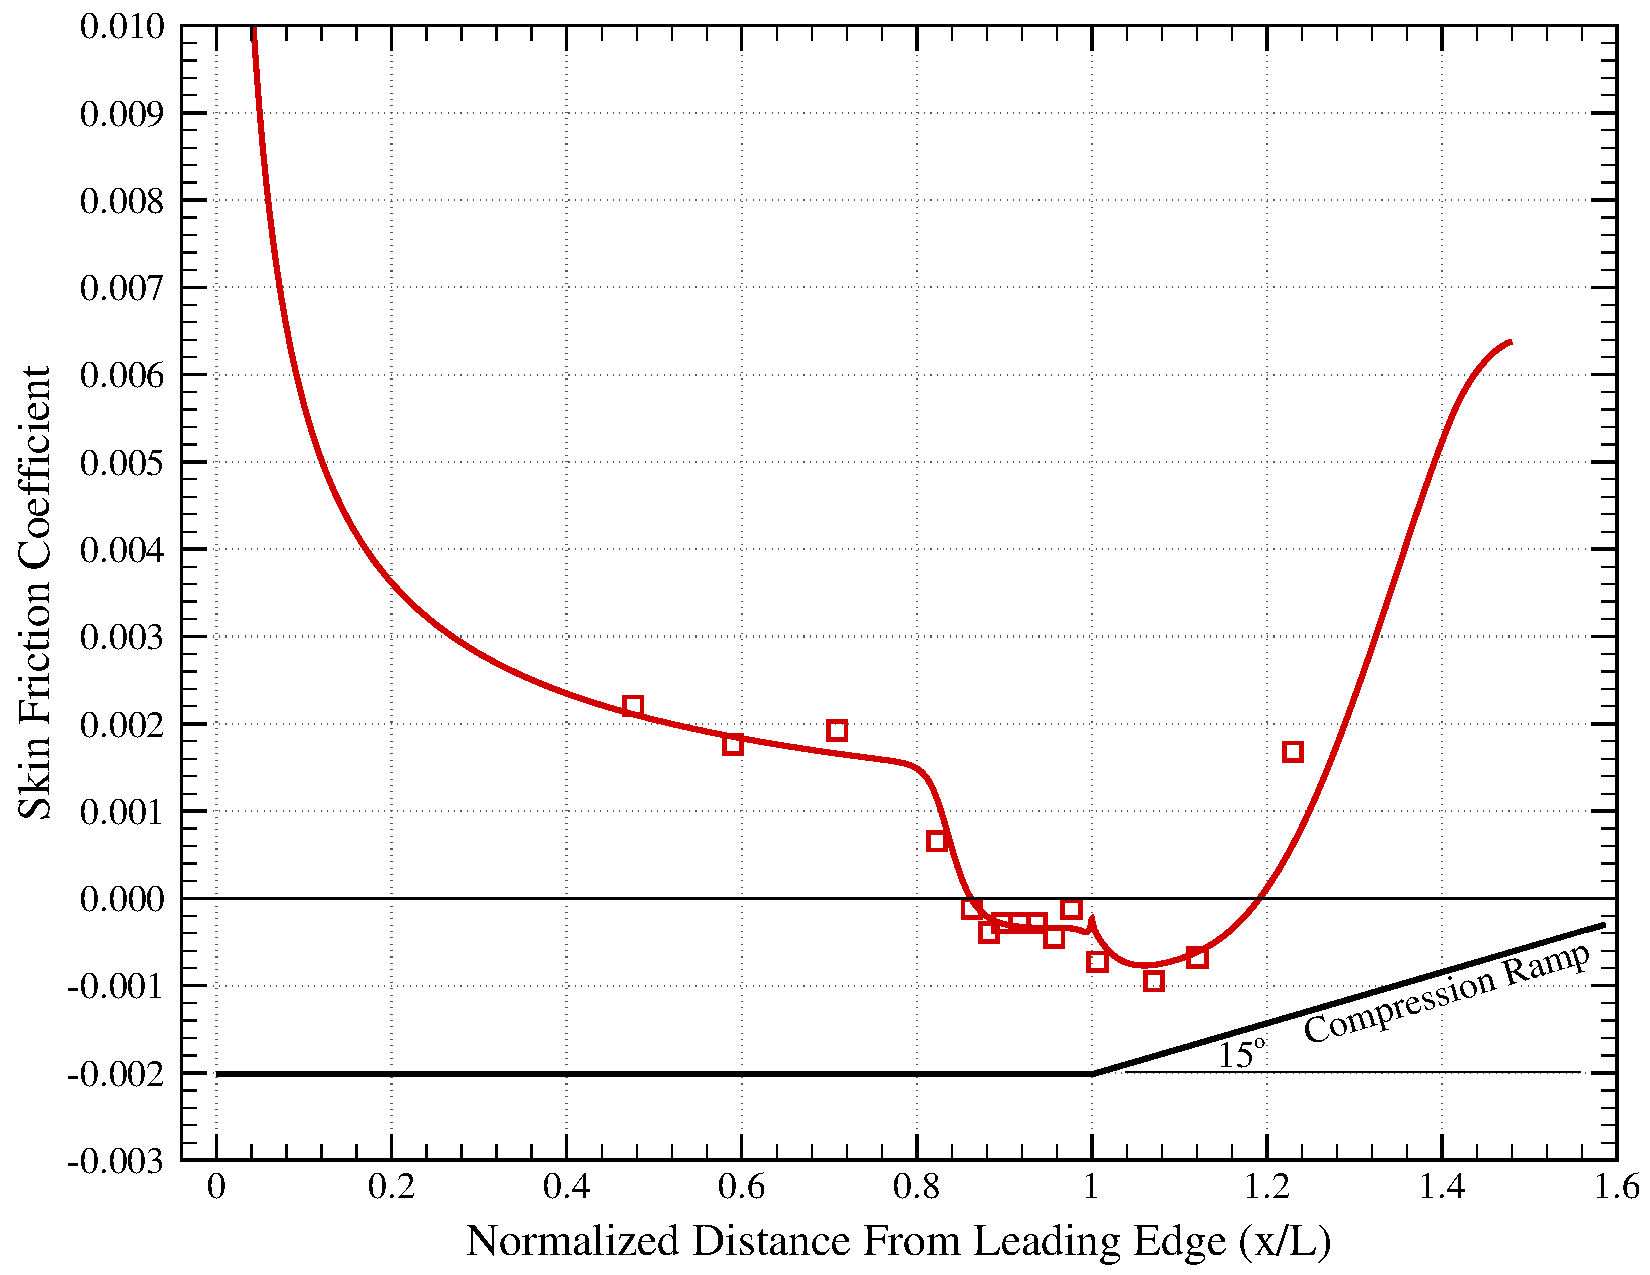
\includegraphics[width=\textwidth]{figures/holden_ramp/skin_friction}
    \caption[Skin friction coefficient comparison with experimental data for hypersonic shock ramp problem]{Skin friction coefficient (solid line) comparison with experimental data (point values) for hypersonic shock ramp problem\label{fig:holden_shock_ramp_exp_cf}}
  \end{center}
\end{figure}


The surface shear is an excellent indicator of the onset of separation which occurs upstream of the compression ramp corner (see Figure~\ref{fig:holden_shock_ramp_recirculation}).  At the separation point the surface shear vanishes.  The attached upstream flow produces a positive shear while the flow in the recirculation region produces a negative shear. Figure~\ref{fig:holden_shock_ramp_exp_cf} plots the nondimensional skin friction coefficient versus the nondimensional distance from the leading edge of the plate.  The skin friction coefficient is defined as
\begin{equation}
  C_f = \frac{\tau_w}{\frac{1}{2} \rho_\infty U_\infty^2}
\end{equation}
where $\tau_w$ is the shear stress which is nondimensionalized with the freestream dynamic pressure.  The experimental and computed values are in general agreement, and the magnitude of the shear is in excellent agreement in the recirculation region (and hence the strength of the recirculation).  Similar results were reported by Lillard and Dries with a completely different flow solver~\cite{lillard_overflow_heating}.

The surface heat transfer is critically important because of the severe heating which can occur in the reattachment region on the compression ramp.  In this region the edge of the boundary layer is subject to a compression fan which markedly thins the boundary layer.  The resulting surface heat transfer obtains a local maximum.  As previously discussed, the compression ramp serves as a conceptual model for a control surface deflected into a hypersonic stream.  In this application it is critically important to understand the magnitude of the reattachment heating because it provides the design environment for the thermal protection system on the control surface.  An example of this is the ``body flap'' on the Space Shuttle Orbiter.  On the body flap the thermal protection system silica tiles are approximately four times thicker than those immediately upstream because of the increased reattachment heating which occurs when the control surface is deflected.

%\clearpage
In Figure~\ref{fig:holden_shock_ramp_exp_st} the computed and measured heat transfer are compared.  The wall heat transfer, $q_{wall}$, is nondimensionalized by means of the Stanton number
\begin{equation}
  St = \frac{q_{wall}}{\rho_\infty U_\infty c_p \left(r T_0 - T_w\right)}
\end{equation}
where $T_0$ is the freestream total temperature, $T_w$ is the surface temperature of the model, $\rho_\infty$ and $U_\infty$ are the freestream density and velocity, and $c_p$ is the freestream specific heat at constant pressure.  The recovery factor, $r$, is assumed equal to one in this case.  
% Holden compression ramp - Stanton number
\begin{figure}[hbtp]
  \begin{center}
    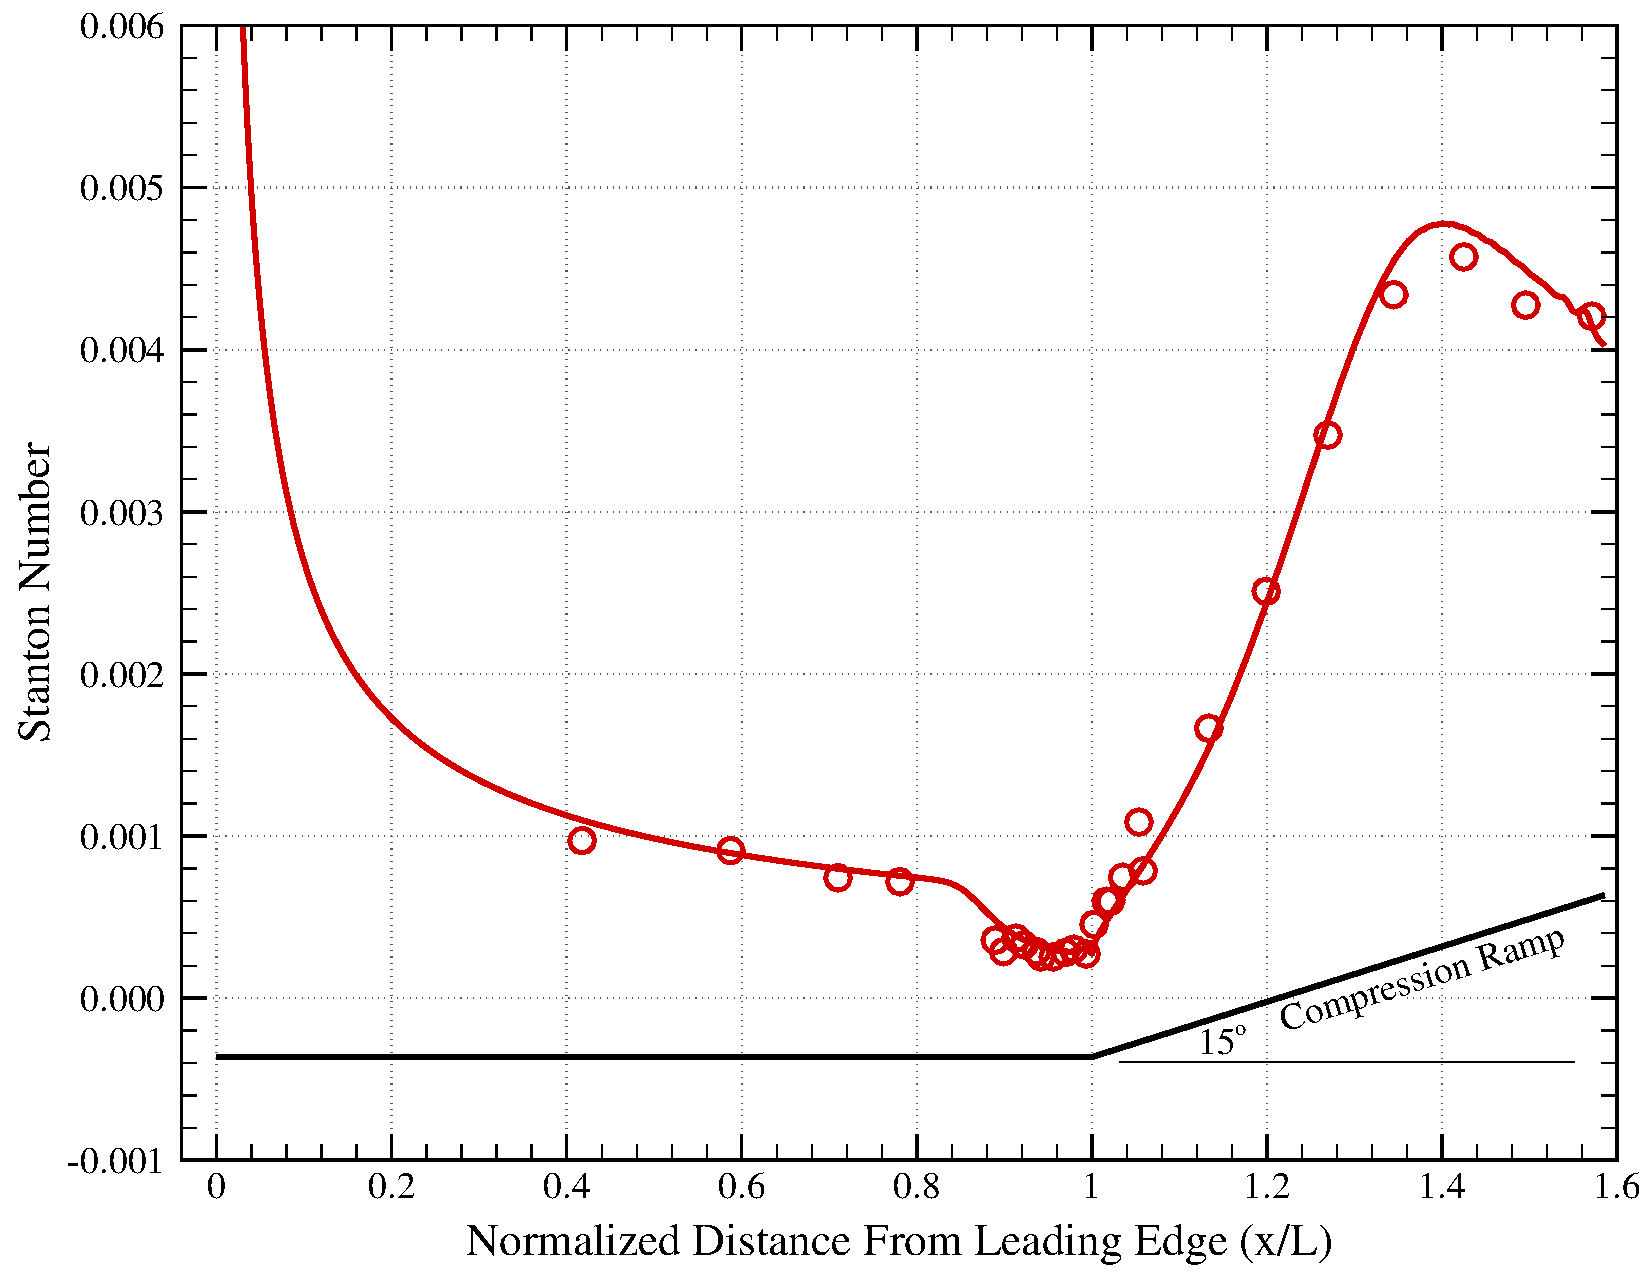
\includegraphics[width=\textwidth]{figures/holden_ramp/stanton}
    \caption{Stanton number comparison with experimental data for hypersonic shock ramp problem\label{fig:holden_shock_ramp_exp_st}}
  \end{center}
\end{figure}

\clearpage
\subsubsection{Convergence}
The simulation was initialized from freestream values and advanced in time using the geometric time advancement scheme described in equations~\eqref{geometric_timestep_growth} and~\eqref{dt_limiting}.  An initial time step of $5\times 10^{-6}$ was used and a geometric growth factor of $r=1.1$ was employed.  The maximum time step was limited to $\Delta t_{\text{max}} = 0.5$.

The normalized unsteady residual versus time step is shown in Figure~\ref{fig:ramp_time_convergence}. 
\begin{figure}[hbtp]
  \begin{center}
    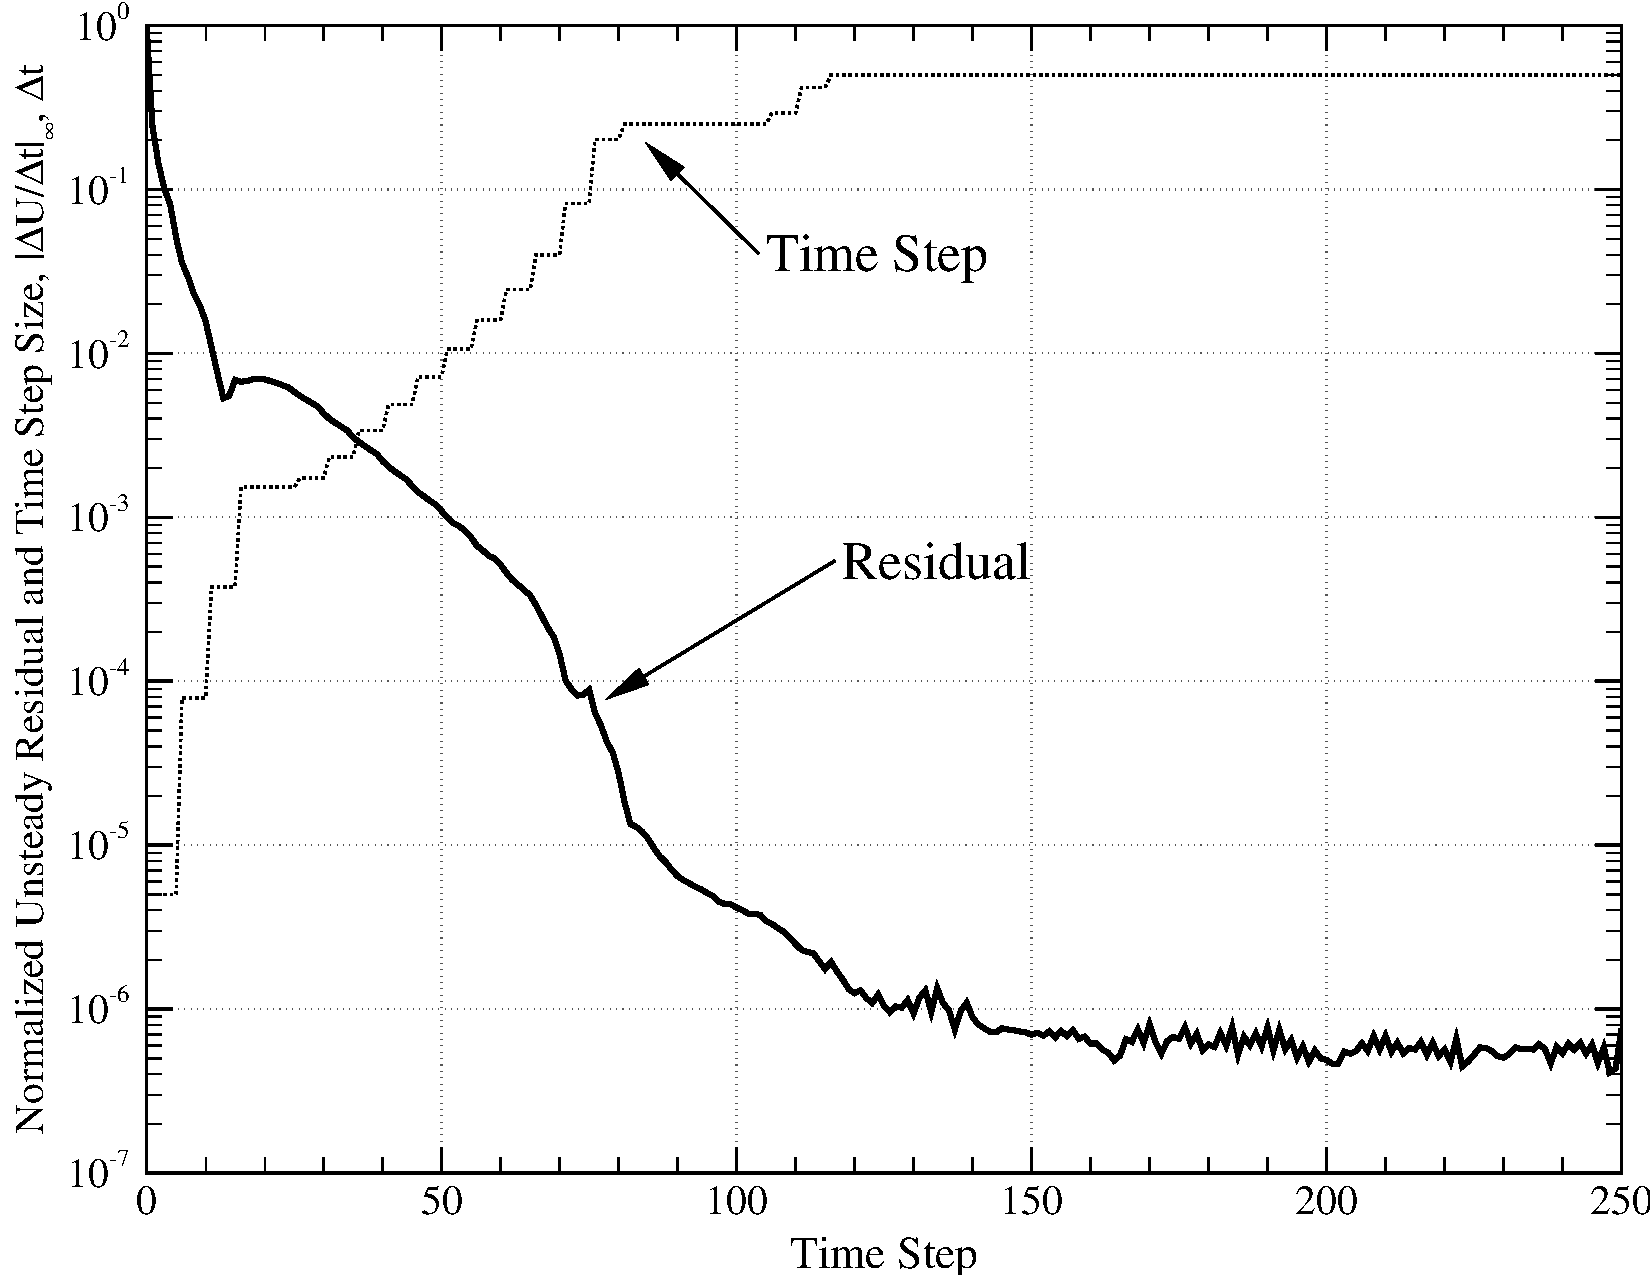
\includegraphics[width=\textwidth]{figures/holden_ramp/time_convergence}
    \caption{Time step convergence history for hypersonic flow over a compression ramp.\label{fig:ramp_time_convergence}}
  \end{center}
\end{figure}
 After an abrupt initial decrease the residual is seen to stagnate at a value of approximately $10^{-6}$.  This is in contrast to the results seen previously for the case of inviscid flow over a cylinder. It should be noted that during this residual stagnation period the solution is visibly steady and both the surface pressure and heat transfer distributions are converged.  Therefore, to investigate the source of the residual stagnation the solution at two different time steps, 200 and 220, was differenced at each node in the mesh and examined.  This procedure indicated that changes on the order of 5--10\% occur at the leading edge of the plate in the vicinity of the slip/stick boundary condition singularity.

The nondimensional time step used in the simulation is also shown in the figure.  Consistent with Equation~\eqref{geometric_timestep_growth}, the time step is seen to increase geometrically with decreasing unsteady residual. Initialized from freestream values, the scheme converges to its steady-state in approximately 150 time steps.  During the first half of this transient the inviscid flow sets up and produces high pressure on the surface of the wedge.  As discussed previously, this induces boundary layer separation, which initiates in the corner and feeds upstream.  During the second half of the transient the separation size gradually increases as the separation point continues to move upstream and the reattachment point moves downstream until steady-state is reached.

\subsubsection{Adaptive Mesh Refinement}
It is clear from the previous global flowfield images that the primary features of this flowfield are the separated recirculation region and the weak shock which develops from the compression ramp surface.  These features are highly localized. The structured grid used in the previous simulations necessarily introduces additional resolution in benign regions of the flow such as downstream of the leading edge shock and upstream of the compression ramp shock.

The primary feature of this flow is the viscous/inviscid interaction set up by the separated region.  The inviscid portion of the domain is adiabatic, but there are considerable non-adiabatic effects in the boundary layer.  In the adiabatic region the total enthalpy in the flow, $H$, is constant, while $H$ will vary appreciably in the viscous/inviscid interaction region. Accordingly, a refinement feature indicator was devised by constructing $\|\grad{H}\|$, the magnitude of total enthalpy gradient on each element in the domain.

Figure~\ref{fig:ramp_amr} details the static temperature and resulting adapted mesh in the vicinity of the compression corner for this case.
\begin{figure}[hbtp]
  \begin{center}
    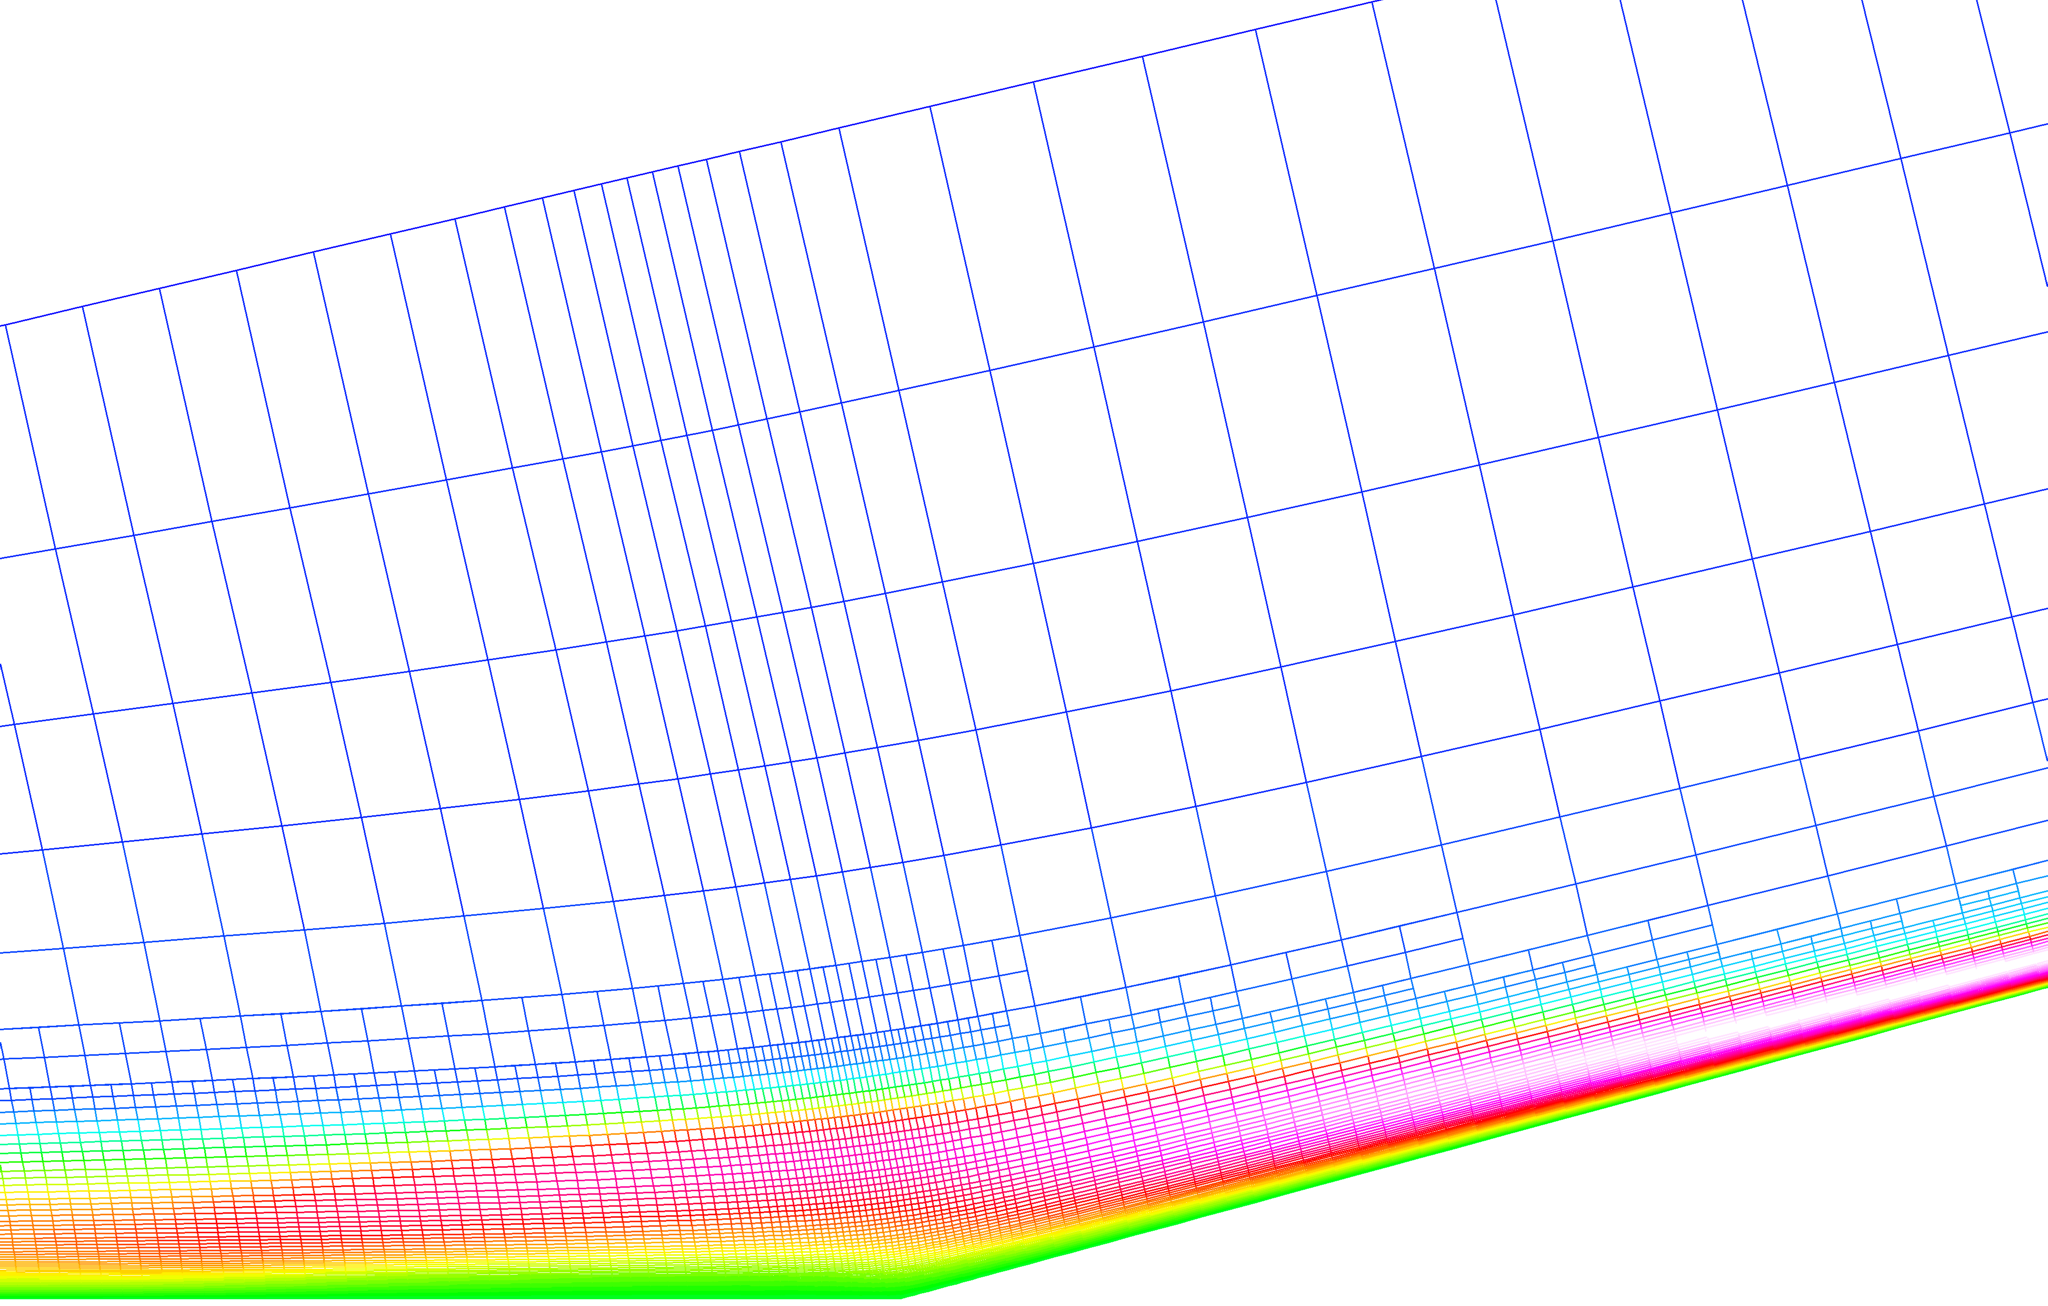
\includegraphics[width=\textwidth]{figures/holden_ramp/amr}
    \caption{Adapted mesh and static temperature contours for hypersonic flow over a compression ramp.\label{fig:ramp_amr}}
  \end{center}
\end{figure}
The initial mesh corresponds to a twice-coarsened version of the baseline mesh used in the previous studies. This coarse mesh contains only 2,940 elements and 3,069 nodes. At each stage in the adaptive refinement algorithm the feature indicator is computed for each active element.  The mean ($f_\text{m}$)  and standard deviation ($\sigma$) are then computed from each element contribution.  Elements which contain values greater than $\left(f_{\text{m}}+\frac{\sigma}{2}\right)$ are selected for refinement, while those with less than $\left(f_{\text{m}}-2\sigma\right)$ are coarsened. 

The final adapted mesh contains approximately 30,000 nodes, which is a 35\% reduction from the baseline mesh.  The flowfield shown in Figure~\ref{fig:ramp_amr} is qualitatively similar to the uniform mesh result. A quantitative comparison is shown in Figure~\ref{fig:ramp_amr_st} in which the Stanton number from the adaptive and uniform simulations are compared.  The two results agree extremely well, with only a small discrepancy in the peak heating value which occurs downstream of the reattachment point.
\begin{figure}[hbtp]
  \begin{center}
    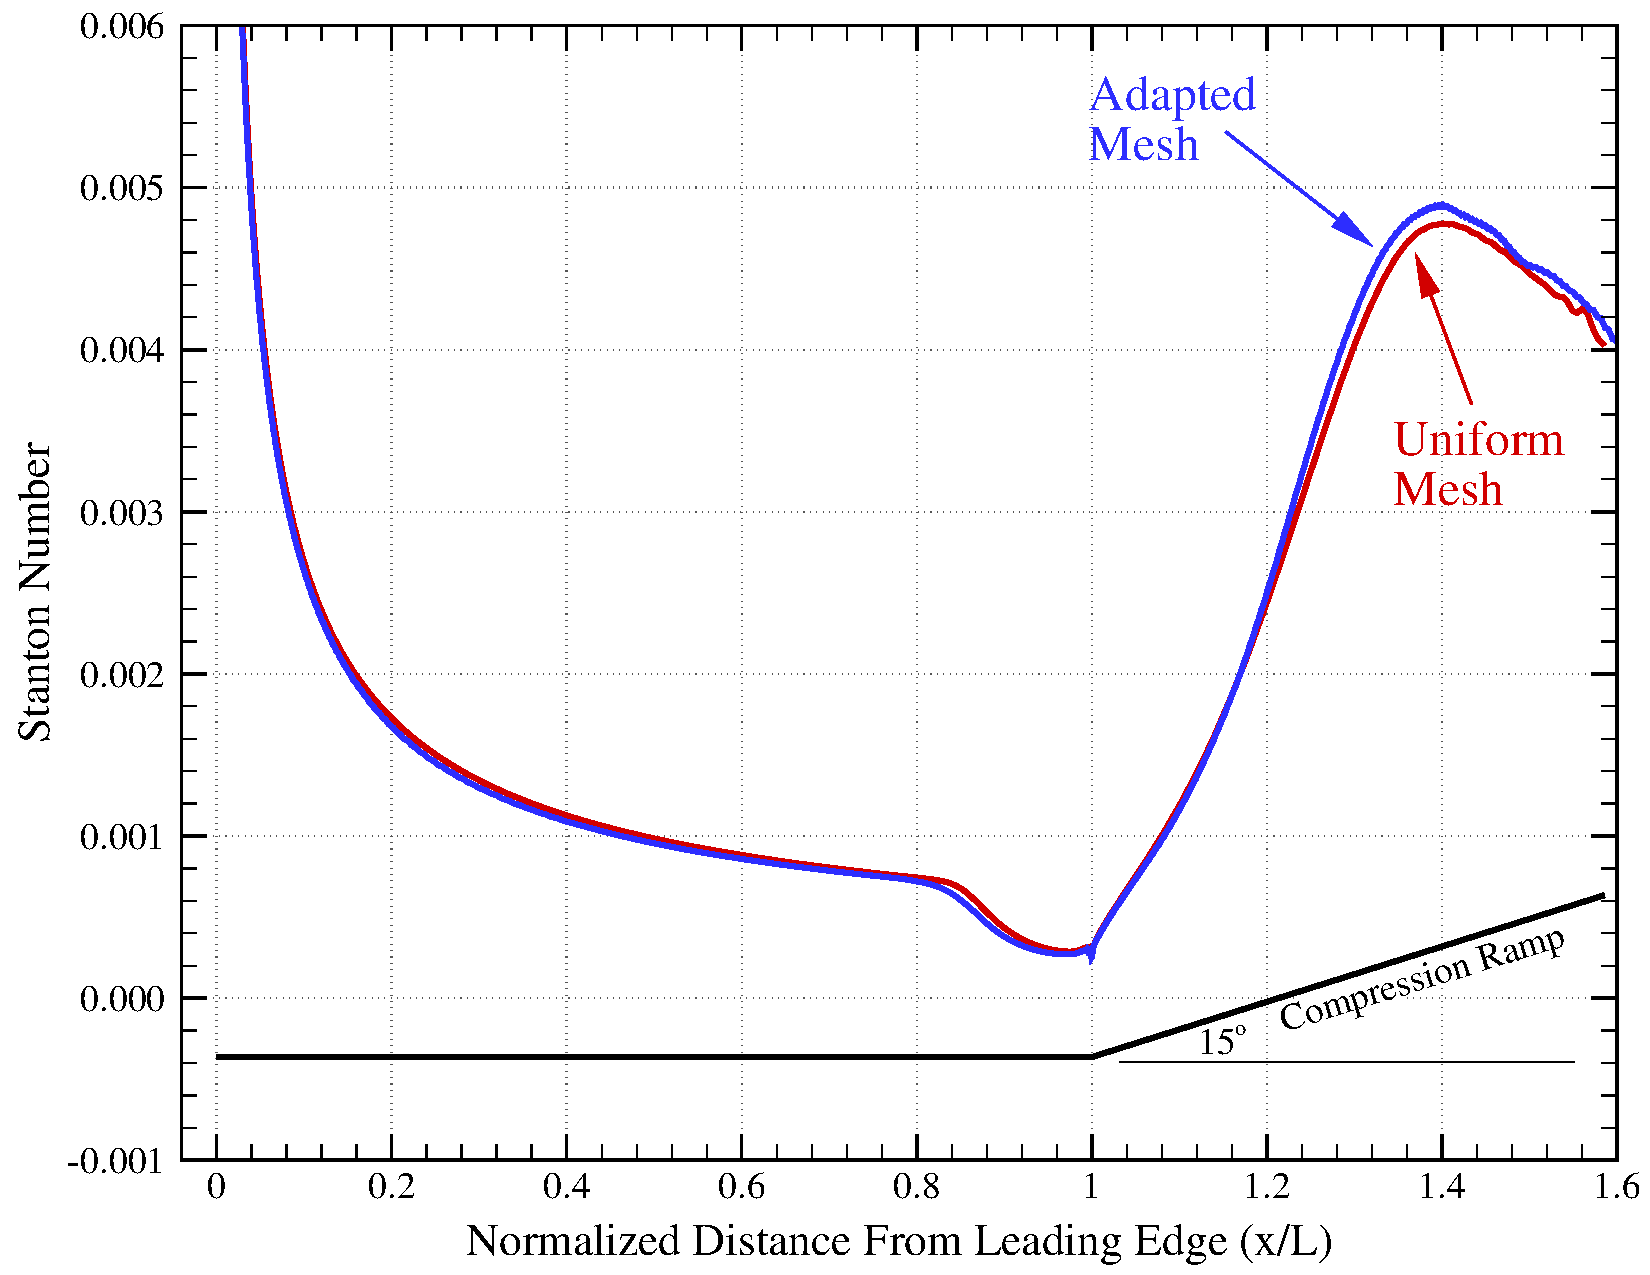
\includegraphics[width=\textwidth]{figures/holden_ramp/amr_st_comp}
    \caption{Stanton number for uniform and adapted meshes for hypersonic flow over a compression ramp.\label{fig:ramp_amr_st}}
  \end{center}
\end{figure}

%%%%%%%%%%%%%%%%%%%%%%%%%%%%%%%%%%%%%%%%%%%%%%%%%%%%%%%%%%%%%%%%%%%%%%%%%%%%%%%
\clearpage
\subsection{Hypersonic Flow over an Axisymmetric Hollow Cylinder-Flare\label{sec:comp_ns_cylinder_flare}}

The $15^\circ$ compression ramp studied in the previous section produces a strong viscous-inviscid interaction in which the inviscid pressure rise caused by the compression ramp induces boundary layer separation and a corresponding recirculation region upstream of the compression surface.  This recirculation region produces a separation shock which does not interact significantly with the model surface.  In this section a stronger interaction on a hollow cylinder-flare model is considered. The availability of high-quality experimental data makes this case valuable for validating the present finite element model.

\subsubsection{Background}
The configuration examined is an axisymmetric hollow cylinder with a flare inclined at $30^\circ$.  (The use of axisymmetric models removes the question of width and edge effects which are an issue for two-dimensional configurations and are particularly problematic for shock interaction problems.) The resulting shock/shock and shock/boundary layer interaction produces a large, localized peak in heat transfer on the model surface.  Experimental data were obtained for this configuration at the Calspan-University of Buffalo Research Center (CUBRC) Large Energy National Shock (LENS) Facility.  An image of the model and schematics depicting the dimensions and instrumentation layout are shown in Figure~\ref{fig:holden_hollow_cylinder}. The freestream conditions for this case are listed in Table~\ref{table:hollow_cylinder-freestream-parameters}.

\begin{figure}[hbtp]
  \begin{center}
    \subfigure[Test Article.]{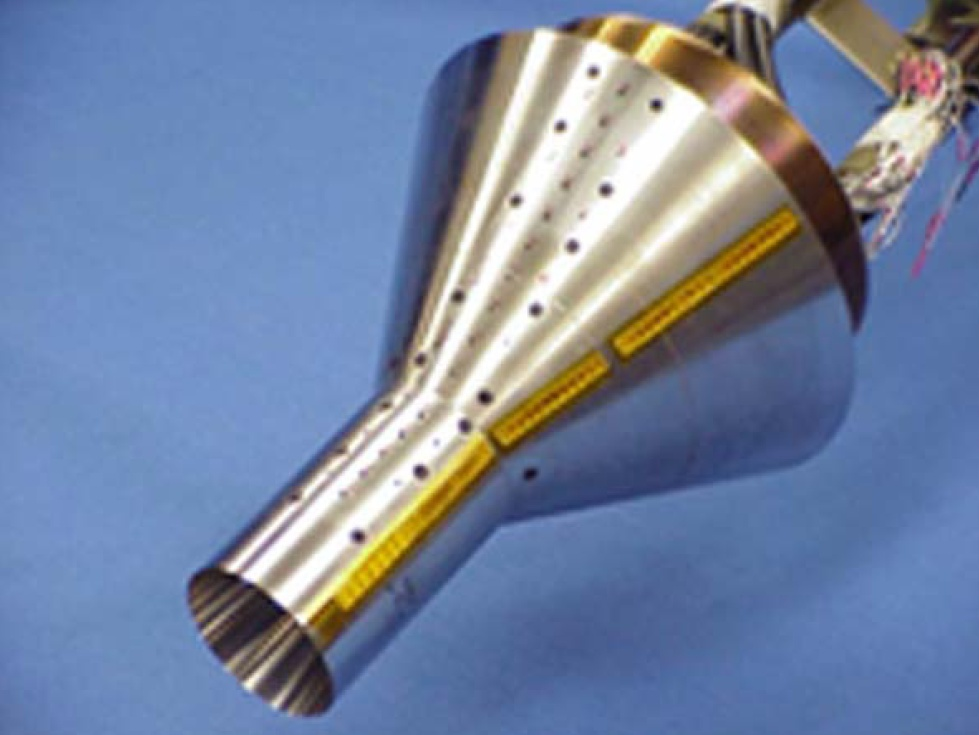
\includegraphics[width=.95\textwidth]{figures/holden_hollow_cylinder/test_article}} \\
    \subfigure[Schematic.  All dimensions are inches.]{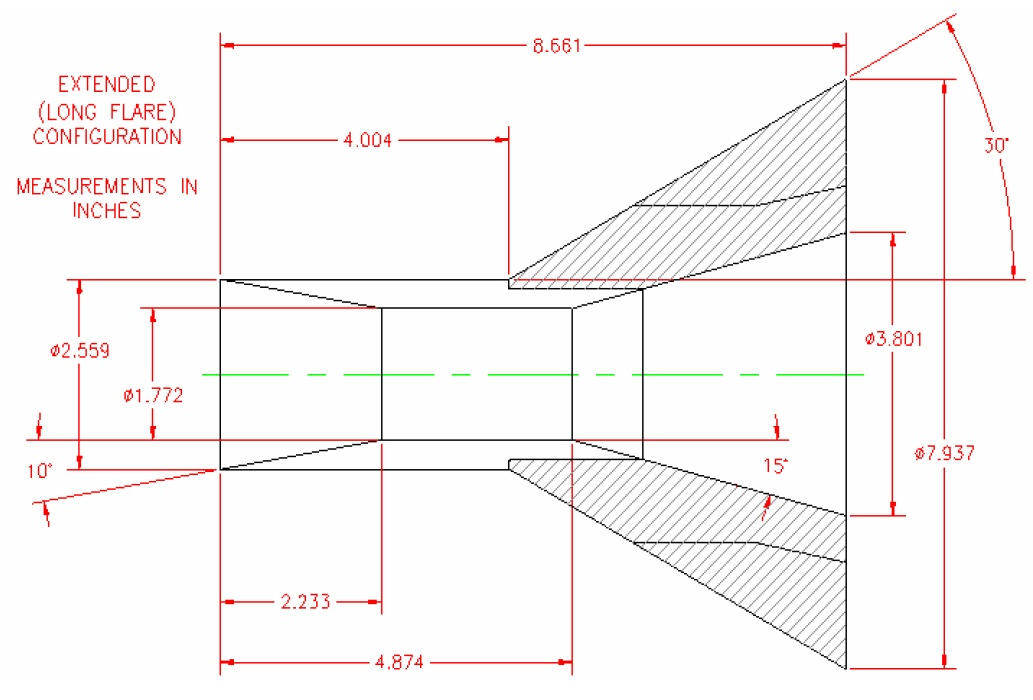
\includegraphics[width=.475\textwidth]{figures/holden_hollow_cylinder/schem_dimensions}}
    \subfigure[Instrumentation Layout.]{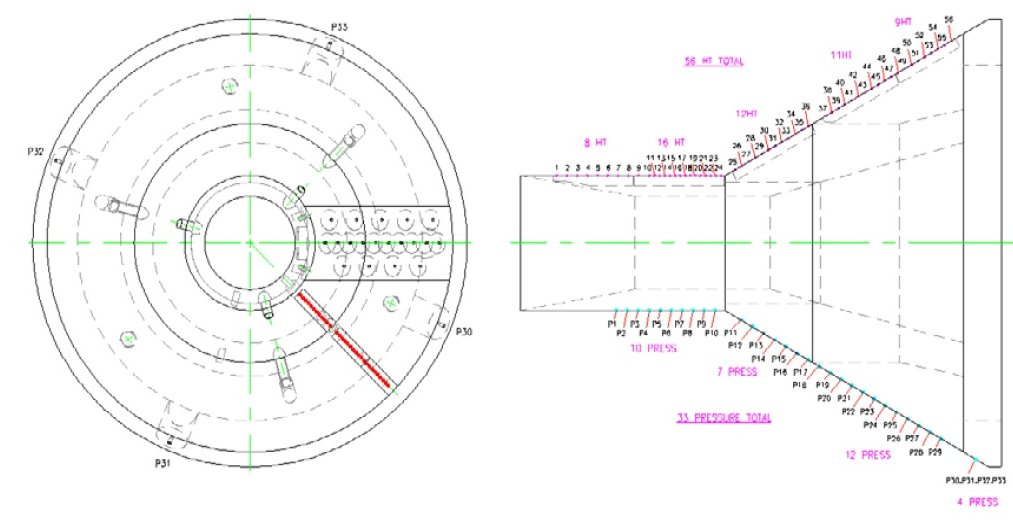
\includegraphics[width=.475\textwidth]{figures/holden_hollow_cylinder/instrumentation}}
    \caption[Hollow cylinder-flare test article and dimensions.]{Hollow cylinder test article and dimensions.\cite{wadhams_holden_AIAA-2004-917}\label{fig:holden_hollow_cylinder}}
  \end{center}
\end{figure}

The model was instrumented with a series of thin-film heat transfer gages and piezoelectric pressure transducers. The reported accuracy of the heat transfer measurements is $\pm 5\%$.  The model was tested in pure Nitrogen to minimize chemical nonequilibrium effects in the flow, which would be appreciable in air at the high freestream enthalpies used in the test~\cite{wadhams_holden_AIAA-2004-917}.  The collected data are extremely valuable for validation of numerical schemes because the flow conditions are such that laminar flow results with minimal chemistry effects.  Hypersonic ground test data in which transition and turbulence or chemical nonequilibrium effects are important are difficult to compare with numerical simulation because the freestream conditions and boundary layer state are often difficult to characterize.

% Holden hollow cylinder - freestream parameters
\begin{table}[hbtp]
  \begin{center}
    \caption[Freestream parameters for hypersonic hollow cylinder-flare benchmark.]{Freestream parameters for hypersonic hollow cylinder-flare benchmark~\cite{gnoffo_AIAA-2001-1025}.\label{table:hollow_cylinder-freestream-parameters}}
    \vspace{1em}
    \begin{tabular}{cccc} \hline \hline
      M$_\infty$ & Re$_L$  & T$_\infty$ & T$_w$     \\
      10.3      & 25,347 & \unit[120.4]{K}   & \unit[295.2]{K} \\ \hline
    \end{tabular}
  \end{center}
\end{table}

Previous numerical studies by Gnoffo~\cite{gnoffo_AIAA-2001-1025} and MacLean~\cite{maclean_AIAA-2004-529} (both of whom assessed the influence of thermal nonequilibrium) have indicated that the assumption of a calorically perfect gas is valid for this case. The transport properties for the flow are given via Sutherland's law with the assumption of constant Prandtl number as described in~\eqref{eq:prandtl}.  For perfect Nitrogen, Sutherland's law takes the form
\begin{equation}
  \label{eq:sutherland_N2}
  \mu_{\text{N$_2$}} =  1.399\times10^{-6}\frac{T^\frac{3}{2}}{T + 106.67}\;\; \unit{Pa\cdot s}
\end{equation}
%Also, these previous studies indicated that the computed flowfield and surface properties are extremely sensitive to the mesh resolution used in the simulation.
%This sensitivity to the computational mesh makes this an excellent case for assessing grid convergence and accuracy of the present finite element solution scheme.

\subsubsection{Computational Mesh}
The computational mesh used for this case is shown in Figure~\ref{fig:holden_hollow_cylinder_mesh}.  It uses two structured grid blocks to encompass the external flow and a portion of the interior just below the sharp leading edge.
\begin{figure}[hbtp]
  \begin{center}
    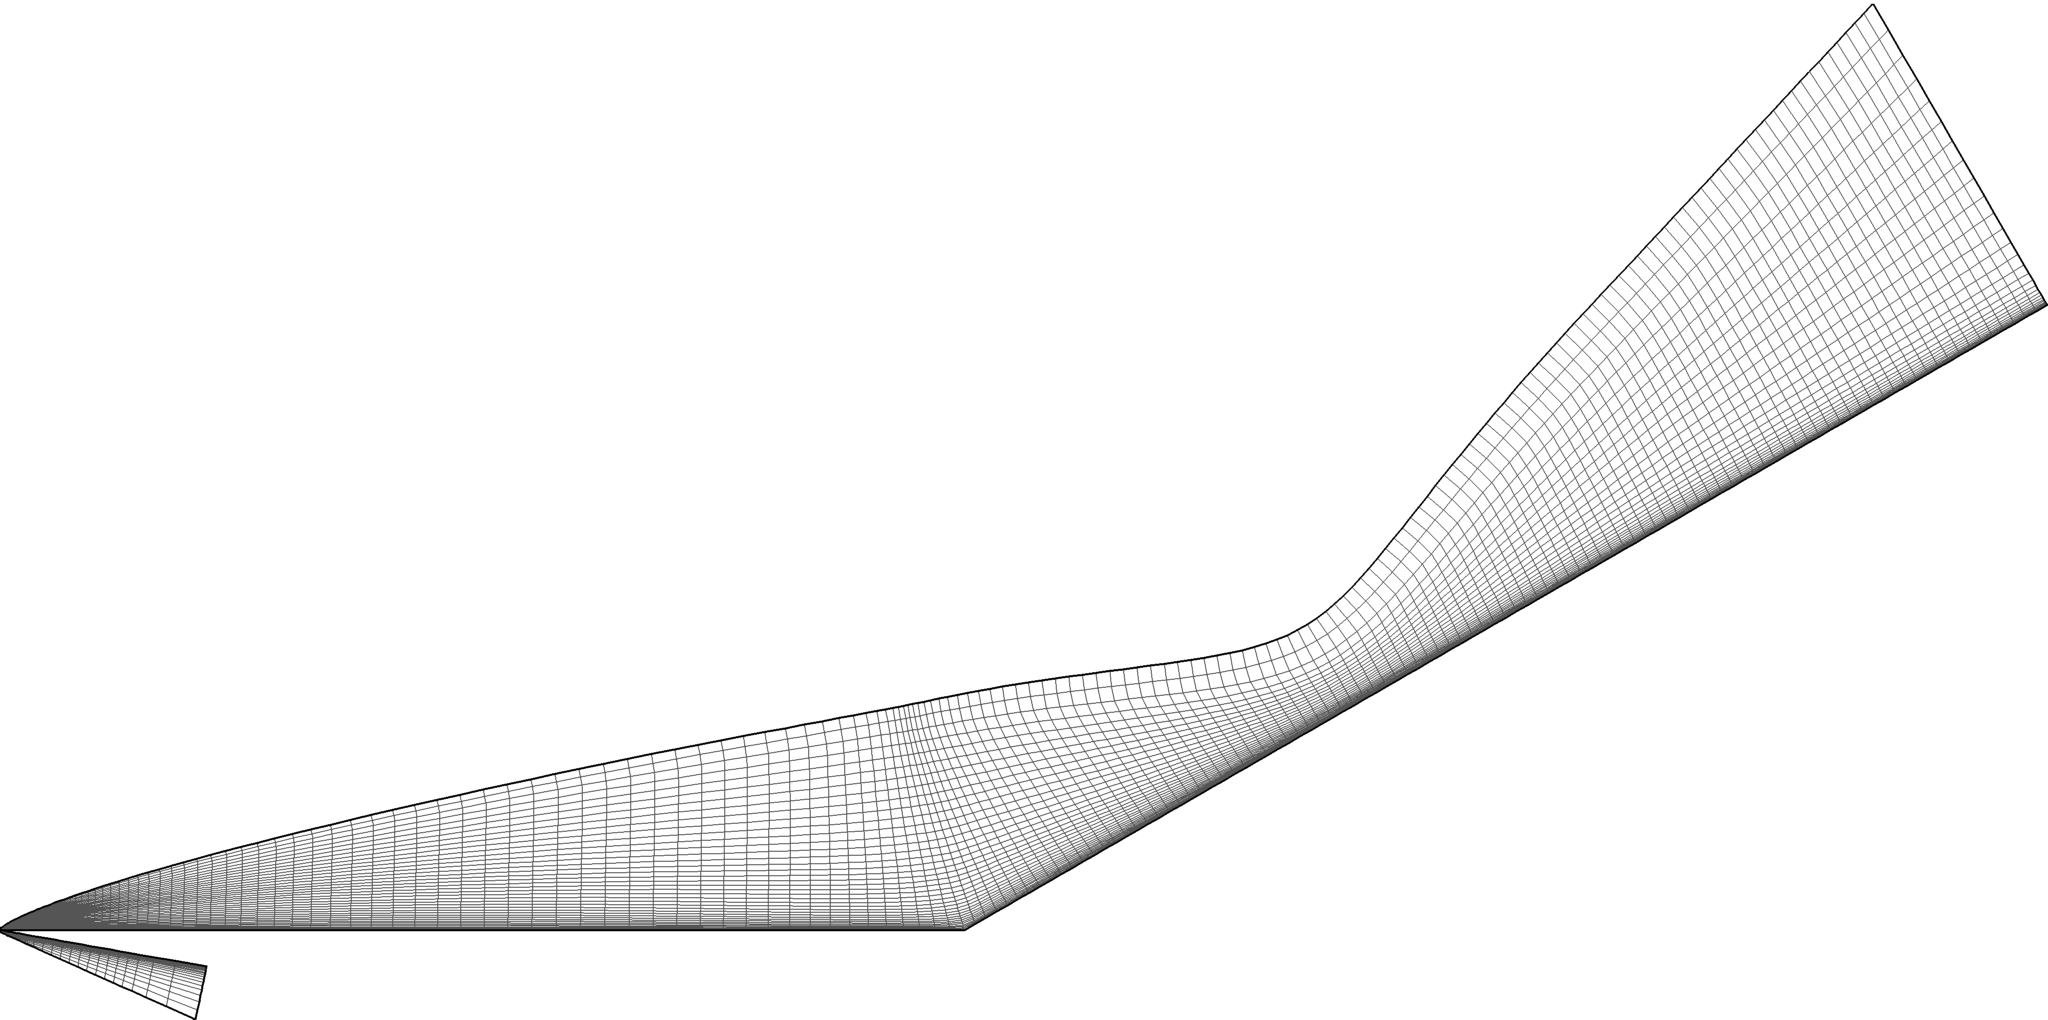
\includegraphics[width=\textwidth]{figures/holden_hollow_cylinder/grid}
    \caption[Baseline computational mesh used for hypersonic flow over a hollow cylinder-flare.]{Baseline computational mesh used for hypersonic flow over a hollow cylinder-flare. (Every-other point is shown)\label{fig:holden_hollow_cylinder_mesh}}
  \end{center}
\end{figure}
Including the interior portion of the domain eliminates the slip/stick velocity boundary condition singularity present in the case of the compression ramp.
The outer boundary of the grid was tailored such that the wall-normal spacing in the reattachment area is minimized, thus allowing for focused resolution in this high gradient region.  As in the previous flat plate case, the height of the outflow boundary was chosen such that the oblique shocks produced by the cylinder displacement thickness and flare would be fully contained within the flow domain. The left and upper boundaries are specified as freestream with essential boundary conditions, and the cylinder-flare is modeled as an isothermal no-slip wall.  The baseline non-adapted mesh used in the simulation contains 45,906 quadrilateral elements with 46,600 nodes, yielding a discrete problem with 186,400 degrees of freedom.


%\clearpage
\subsubsection{Results}
Figures~\ref{fig:holden_hollow_cylinder_global_T}--\ref{fig:holden_hollow_cylinder_global_M} depict the global flowfield for this case.  All figures clearly depict a weak leading edge shock caused by boundary layer displacement effects which merges with a separation shock.  This merged shock then impinges on the flare surface.  These features will be discussed in more detail in the context of the specific field variables shown in the figures.

\clearpage
Several important flow features are evident from the static temperature field shown in Figure~\ref{fig:holden_hollow_cylinder_global_T}.
\begin{figure}[hbtp]
  \begin{center}
    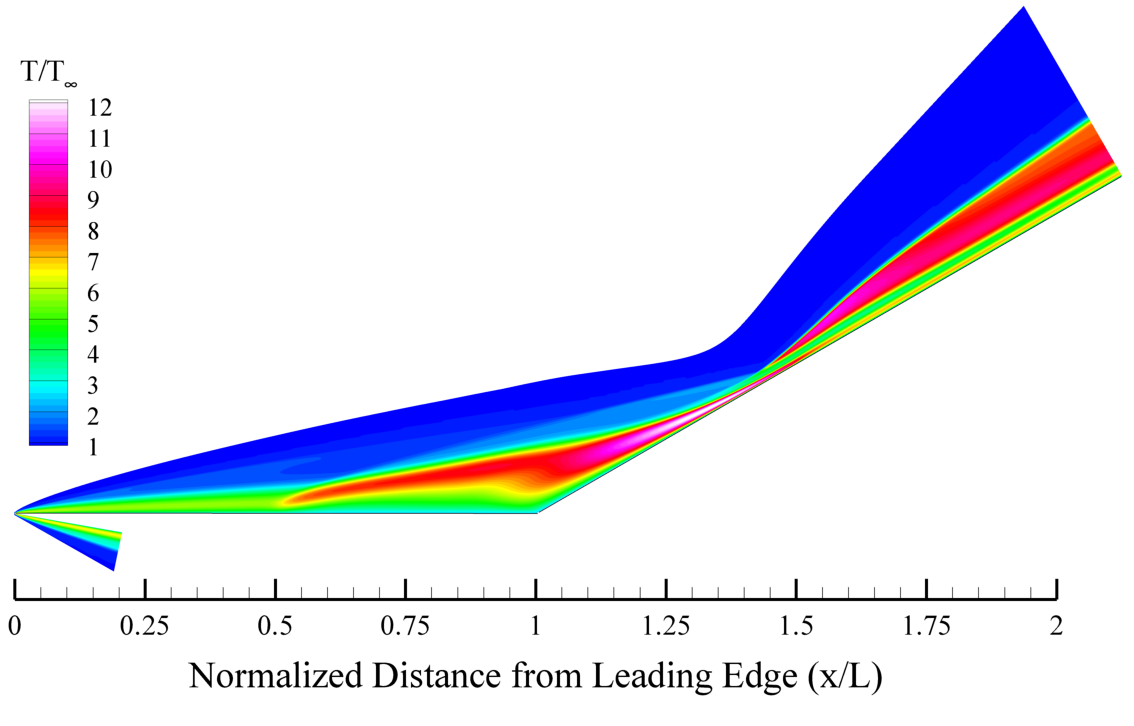
\includegraphics[width=\textwidth]{figures/holden_hollow_cylinder/T}
    \caption{Illustration of flowfield for hypersonic hollow cylinder-flare shock interaction problem: nondimensional static temperature.\label{fig:holden_hollow_cylinder_global_T}}
  \end{center}
\end{figure}
 A weak shock develops at the leading edge of the hollow cylinder due to boundary layer displacement effects.  The flow separates at approximately (x/L) of 0.5 and creates a separation shock which coalesces with the leading edge shock.  The separation/leading edge merged shock is then seen to impinge on the conical section in the reattachment region.  The strong temperature gradient in the reattachment region at (x/L) of 1.4 is clearly evident.  The peak temperature in the reattachment region is \unit[1450]{K} (approximately 12 times the freestream value).  Clearly these elevated temperatures would cause significant excitation and dissociation of O$_2$ in air, however these effects are mitigated by using N$_2$ as the test gas.  

\clearpage
 Figure~\ref{fig:holden_hollow_cylinder_global_P} shows the flowfield  nondimensional static pressure for this case.  There is clearly a strong, local increase in pressure in the interaction/reattachment region.  
\begin{figure}[hbtp]
  \begin{center}
    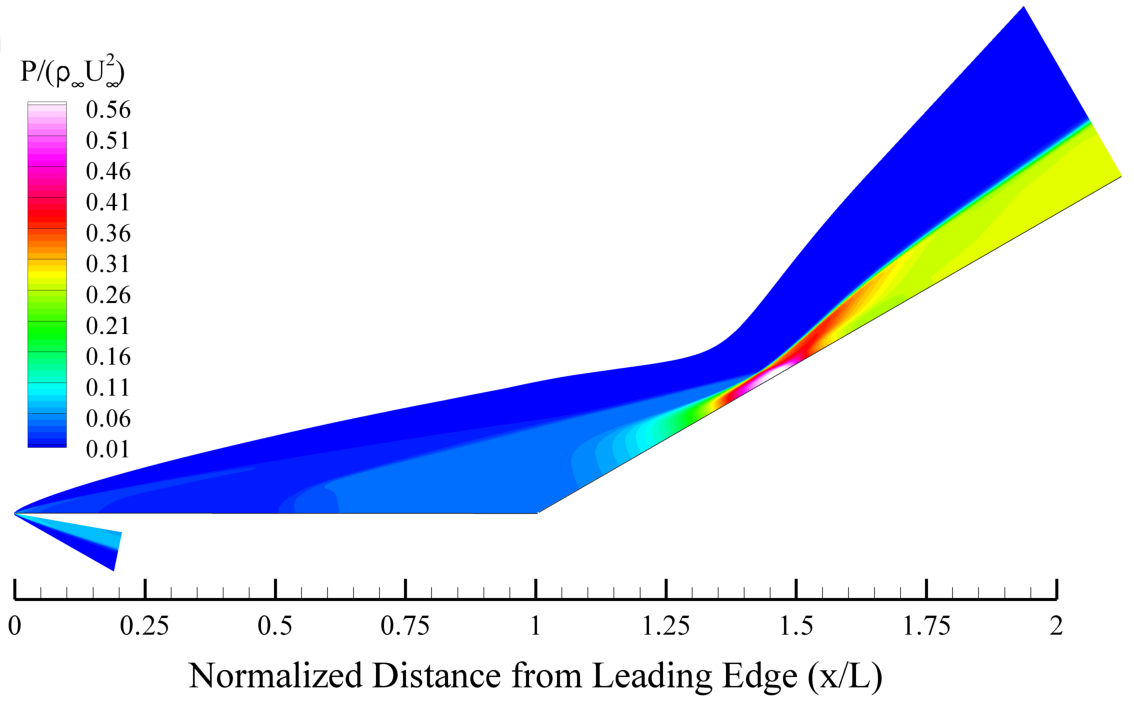
\includegraphics[width=\textwidth]{figures/holden_hollow_cylinder/P}
    \caption{Illustration of flowfield for hypersonic hollow cylinder-flare shock interaction problem: nondimensional static pressure.\label{fig:holden_hollow_cylinder_global_P}}
  \end{center}
\end{figure}
Further, the adverse pressure gradient on the forward portion of the cone is evident.  It is this adverse pressure gradient that induces boundary layer separation.  In turn, the separated boundary layer induces a shock wave which interacts with the reattachment region, resulting in a tight coupling between the size of the separation region, strength of the separation shock, and the magnitude of the adverse pressure gradient.  In this way this problem serves as an excellent test for a numeric scheme because an error in modeling any one of these features can be magnified by the inherit nonlinear couplings in the flowfield response.

\clearpage
Figure~\ref{fig:holden_hollow_cylinder_global_M} shows the Mach number distribution. The flowfield is largely supersonic with the exception of the recirculation region.
\begin{figure}[hbtp]
  \begin{center}
    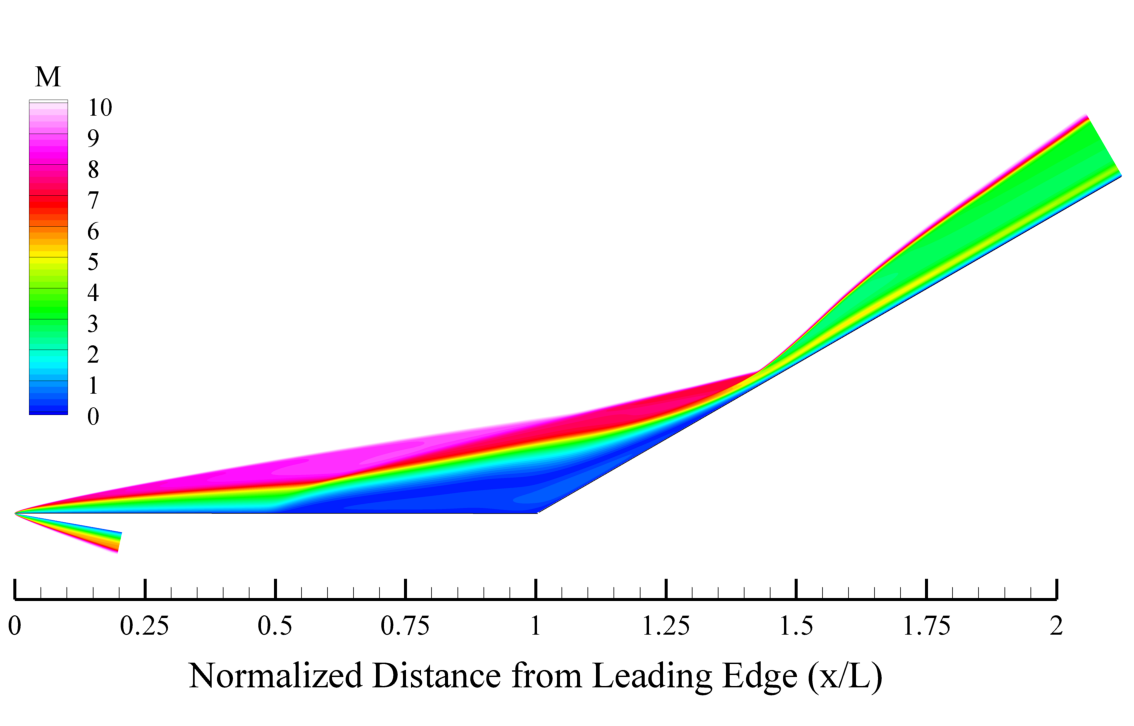
\includegraphics[width=\textwidth]{figures/holden_hollow_cylinder/M}
    \caption{Illustration of flowfield for hypersonic hollow cylinder-flare shock interaction problem: Mach number.\label{fig:holden_hollow_cylinder_global_M}}
  \end{center}
\end{figure}
 The weak leading edge shock decelerates the flow from Mach~10.3 to Mach~9, and the conical section shock decelerates the flow to approximately Mach~4.  The outflow is supersonic in all but the extreme near-wall region, hence the use of an extrapolation outflow boundary condition is justified.

\clearpage
Figure~\ref{fig:hollow_cylinder_ch_cp} shows a comparison between measured and computed heat transfer and pressure coefficients. The heat transfer coefficient is defined as
\begin{equation}
  C_H = \frac{q_{wall}}{\frac{1}{2} \rho_\infty U_\infty^3}
\end{equation}
which nondimensionalizes the wall heat flux by the freestream maximum energy flux. The pressure coefficient is defined as
\begin{equation}
  C_p = \frac{P-P_\infty}{\frac{1}{2} \rho_\infty U_\infty^2}
\end{equation}
which nondimensionalizes the difference between the local and freestream pressure by the freestream dynamic pressure.
\begin{figure}[hbtp]
  \begin{center}
    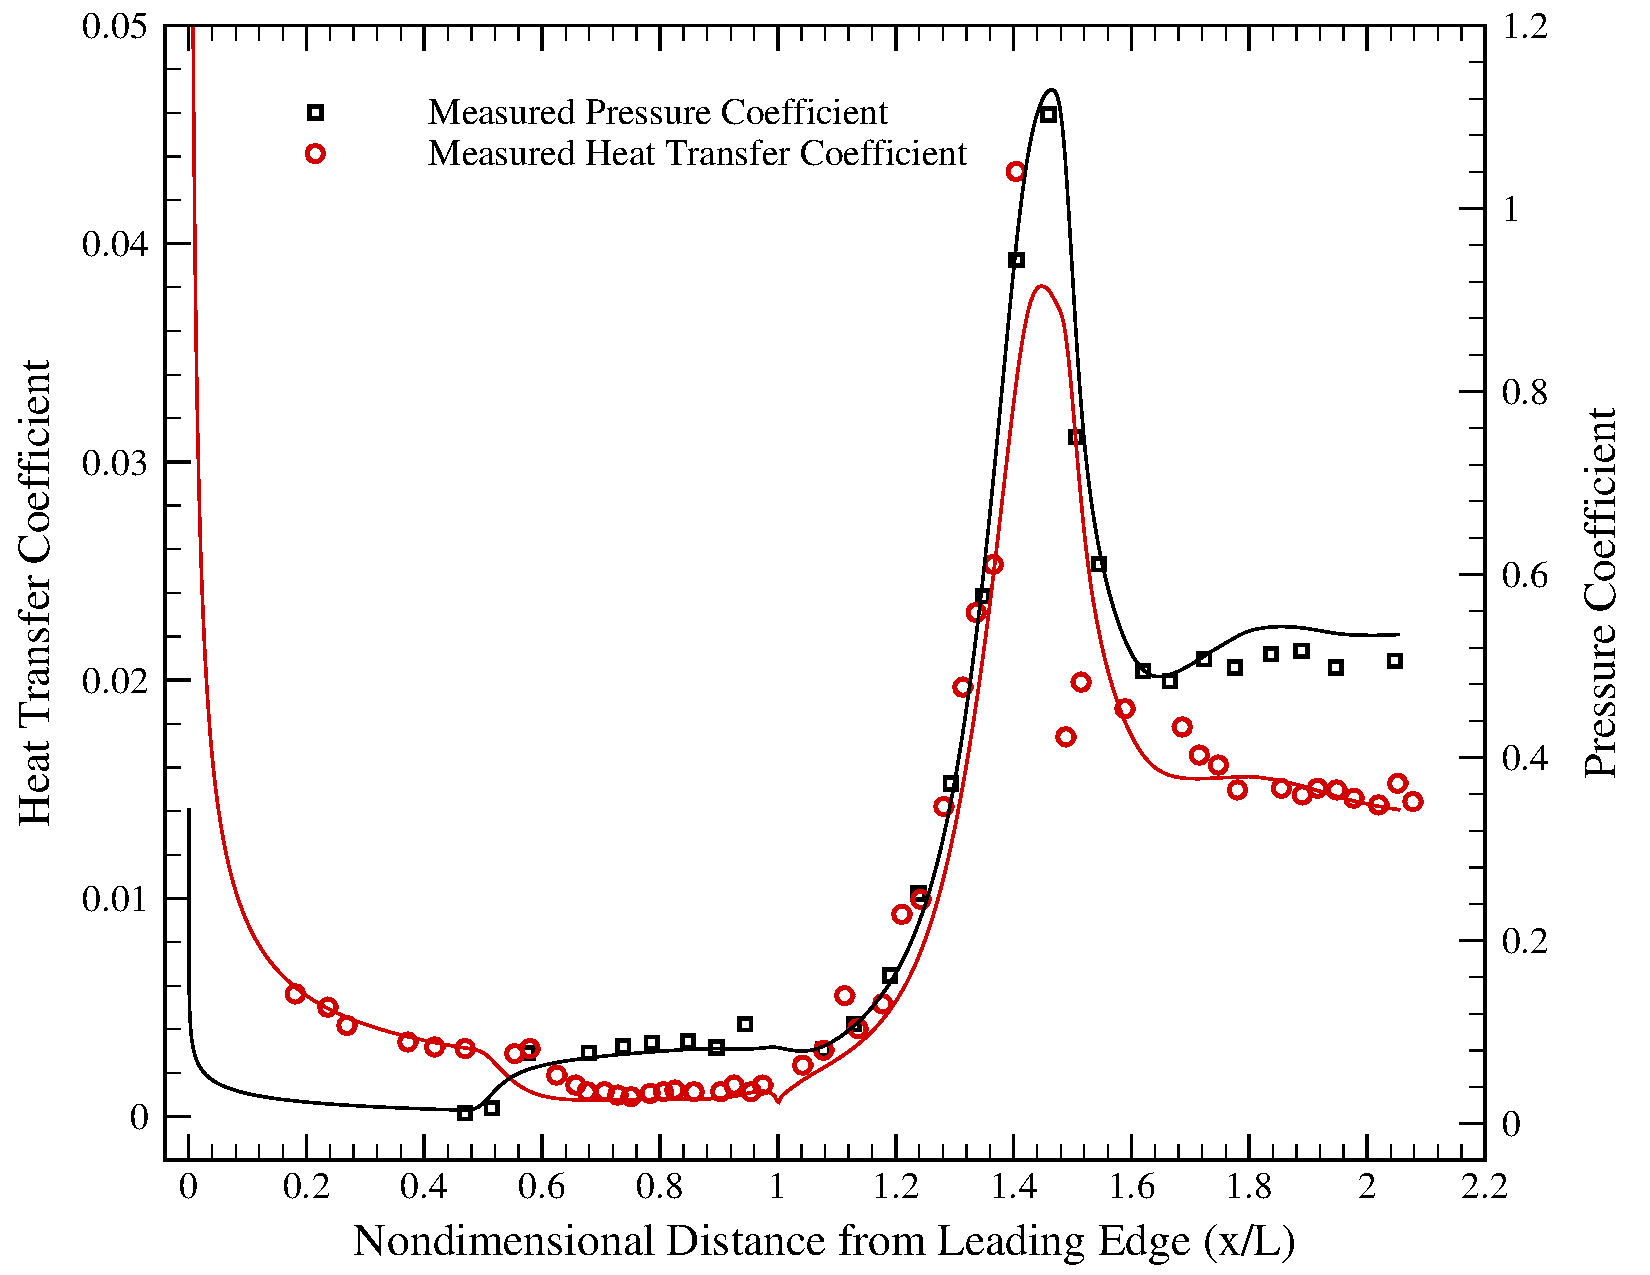
\includegraphics[width=\textwidth]{figures/holden_hollow_cylinder/ch_cp_comparison}
    \caption[Comparison of measured and computed heat transfer and pressure coefficients for hollow cylinder-flare configuration.]{Comparison of measured and computed heat transfer and pressure coefficients for hollow cylinder-flare configuration.\label{fig:hollow_cylinder_ch_cp}}
  \end{center}  
\end{figure}

Both the trends and magnitudes of the experimental data are well captured by the numerical solution.  Separation is clearly evident at (x/L) of 0.5 as indicated by the increase in pressure coefficient and corresponding decrease in surface heat transfer.  The extreme wall-normal temperature gradients in the reattachment region is reflected in increased heat transfer to the surface.  The measured peak heat transfer exceeds the computed value. However, similar behavior was seen by MacLean~\cite{maclean_AIAA-2004-529} with two completely different flow solvers. This lends credibility to the current numerical results. During the transient startup phase, prior to achieving steady-state, the forward extent of the separation region increases while the location of the reattachment moves downstream. The peak heating in the reattachment region decreases as the extent of the separated region approaches steady-state.   This transient behavior is obviously present in the experimental configuration as well. Additionally, obtaining a steady response for data sampling is difficult.  This is especially the case in the reattachment region, so it is possible that the experimental data correspond to a snapshot of a slowly evolving transient flowfield.

\clearpage
\subsubsection{Adaptive Mesh Refinement}
The adaptive procedure outlined previously for the case of hypersonic flow over a compression ramp is again applied to this case.  The total enthalpy gradient is used as a feature indicator to focus mesh refinement in the viscous/inviscid and shock/boundary layer interaction regions.  The adapted mesh and static temperature field are shown in Figure~\ref{fig:hollow_cylinder_amr}.
\begin{figure}[hbtp]
  \begin{center}
    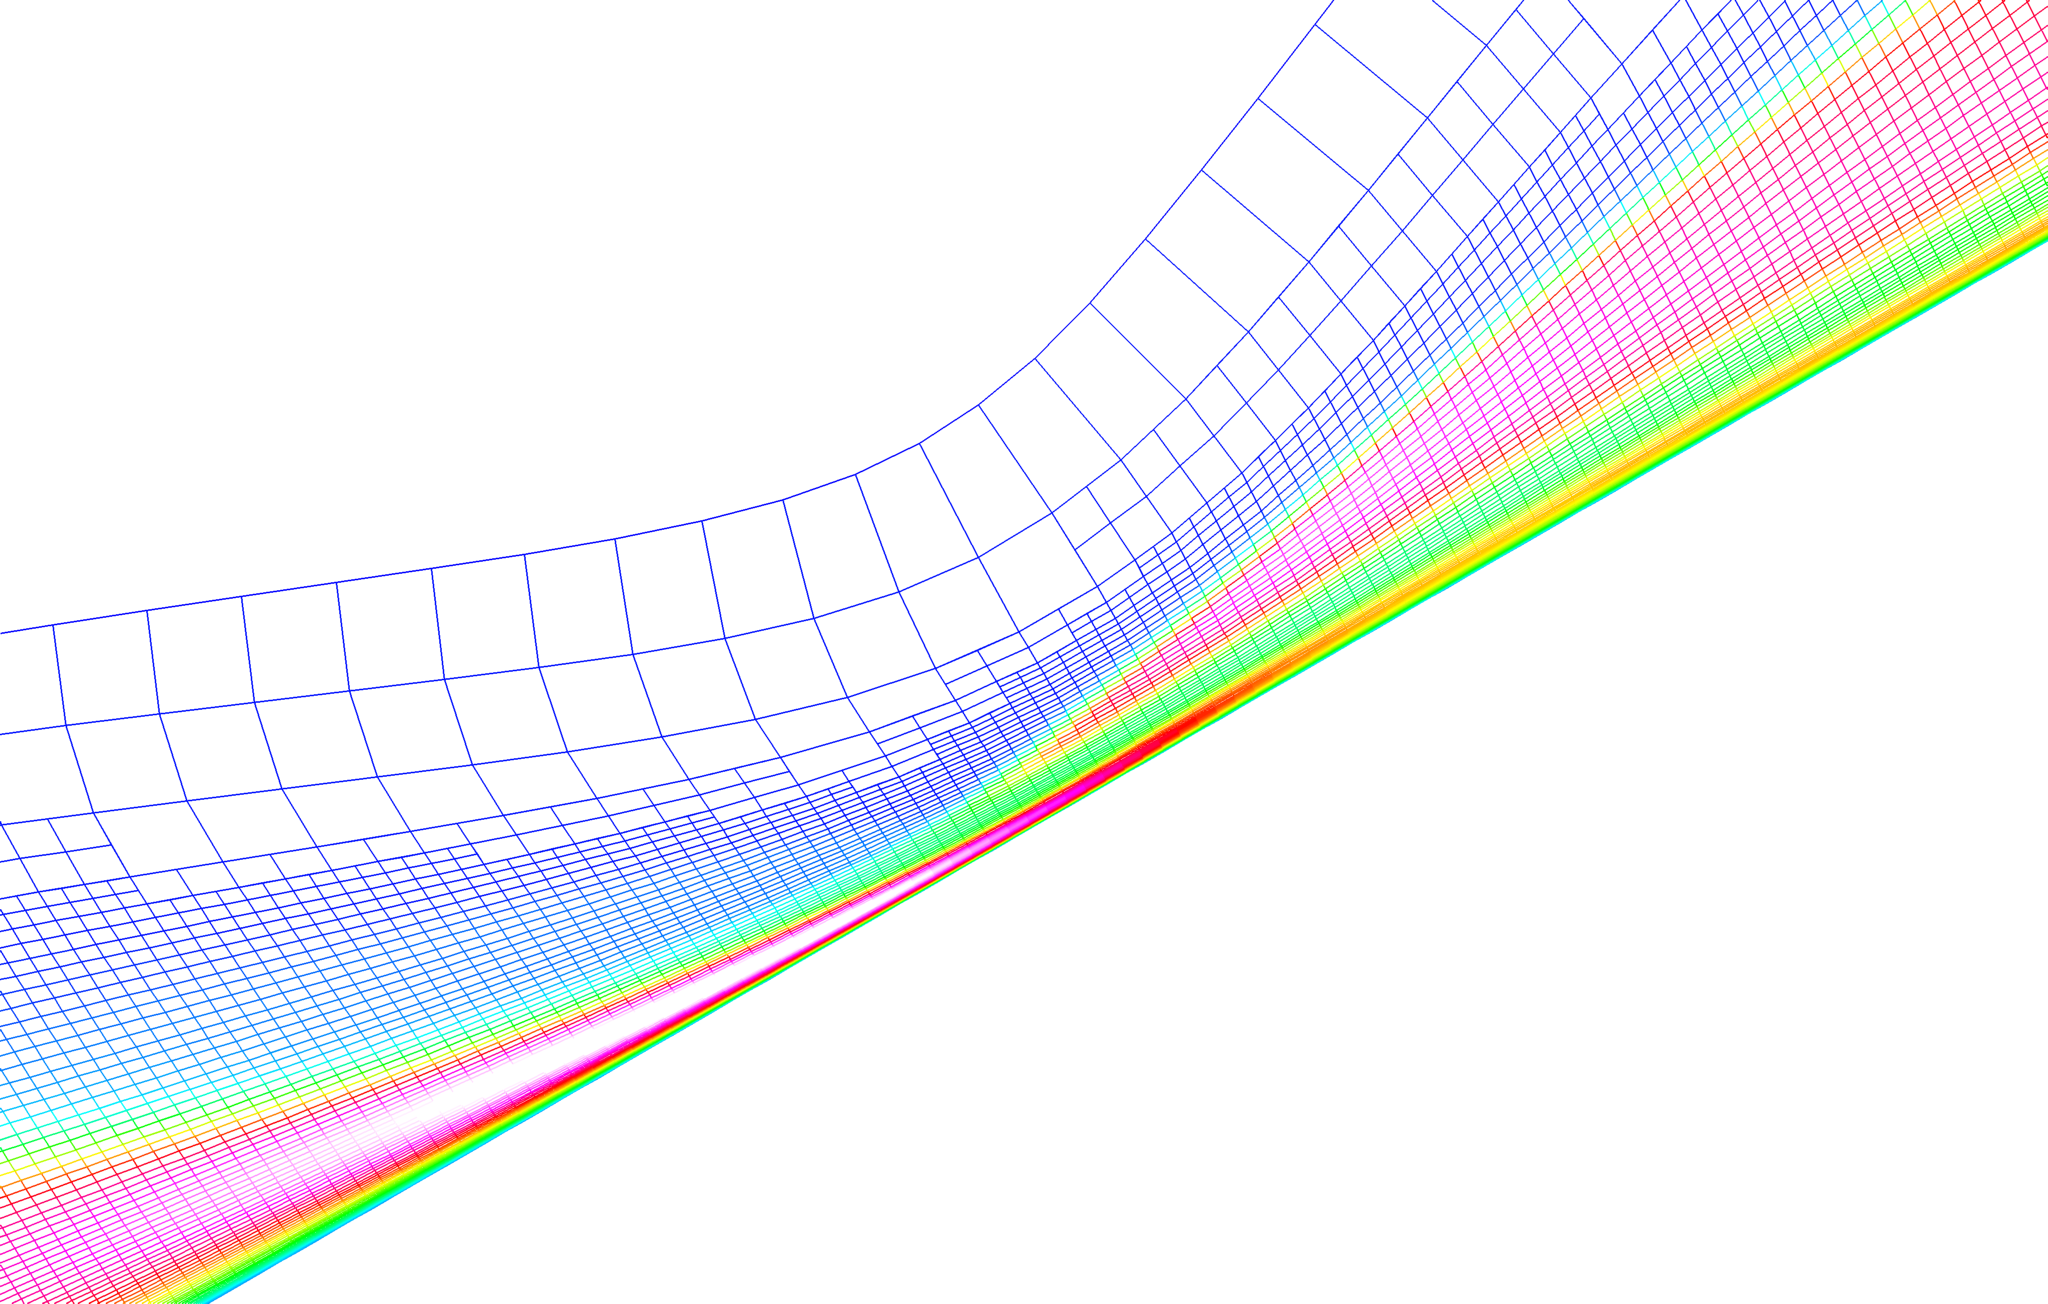
\includegraphics[width=\textwidth]{figures/holden_hollow_cylinder/amr2}
    \caption{Adapted mesh and static temperature contours for the reattachment region of a  hypersonic flow over a hollow cylinder-flare.\label{fig:hollow_cylinder_amr}}
  \end{center}
\end{figure}
The background mesh is visible in the far-field portion of the domain and corresponds to a twice-coarsened version (containing a factor of 16 fewer elements) of the baseline, uniform mesh. The adapted mesh contains approximately 30\% fewer degrees of freedom than the uniform mesh.
The surface pressure and heat transfer for the adapted mesh are visually identical to the uniform case and thus are not shown here.  



%%%%%%%%%%%%%%%%%%%%%%%%%%%%%%%%%%%%%%%%%%%%%%%%%%%%%%%%%%%%%%%%%%%%%%%%%%%%%%%
\clearpage
\subsection{Hypersonic Flow over an Axisymmetric Double Cone\label{sec:comp_ns_double_cone}}
Another experimental case with extensive data is that of a
geometrically axisymmetric biconic, or double cone model. The double
cone has been extensively studied and computationally modeled because
of the complex shock interaction structure that results from the
compound geometric angle.

Previous research has shown that this simple geometry can yield a very complex and potentially unsteady flowfield response~\cite{nompelis_candler_holden_double_cone,AEDC_HVWT9_double_cone}.  Initial experimental testing was performed in a Nitrogen stream at CUBRC for a range of freestream Reynolds numbers~\cite{holden_wadhams_AIAA-2003-1137}.  Subsequent analysis by Nompelis et al.~\cite{nompelis_candler_holden_double_cone} showed that certain aspects of the experimental results could be best explained by accounting for vibrational nonequilibrium in the freestream.  This observation was a result of detailed analysis which accounted for the nonequilibrium expansion within the nozzle to arrive at the freestream conditions which were then fixed as inflow conditions for analysis of the double cone.  These observations are in agreement with previous experimental and computational investigations of double cone flow performed by Olejniczak~\cite{olejniczak_dissertation} which highlighted the sensitivity of these flows to chemical nonequilibrium effects.

Following this discovery, subsequent testing was performed at the Arnold Engineering Development Center (AEDC) Hypervelocity Wind Tunnel Number~9 (HVWT9), which is located in White Oaks, Maryland.  This facility provides relatively long run times (on the order of seconds) which allows for data to be obtained for a long period of time at a range of flow conditions.  The tunnel also uses Nitrogen as its working fluid, hence the results obtained at CUBRC were of interest to AEDC test engineers. The same model was tested in HVWT9 to investigate the potential impacts of vibrational nonequilibrium.  Contrary to the CUBRC experience, however, flow in the test section of HVWT9 was found to behave as a calorically perfect gas for all tested conditions. Also, significant unsteadiness was observed in the flowfield~\cite{AEDC_HVWT9_double_cone}. It is hypothesized here that the perfect-gas nature of the flow in the AEDC facility is due to intrinsic differences in the two facilities. (LENS is a shock-driven impulse facility while HVWT9 is a blow-down tunnel.) The source of unsteadiness will be considered further in this work and is the subject of Section~\ref{sec:comp_ns_double_cone_unsteady}.

\subsubsection{CUBRC Blunt Double Cone}
For the CUBRC code validation database, the double cone was selected to have a $25^\circ$ and $55^\circ$ primary and secondary half-angle, respectively. This particular choice is interesting in that the forecone $25^\circ$ half-angle admits an attached oblique shock, while the $55^\circ$ aftcone half-angle is sufficiently steep that an attached shock is not possible.  Therefore, the aftcone produces a detached bow shock which will be intersected by the forecone oblique shock.

Code validation studies for  four separate nose configurations are available. Here, the blunt nose tip radius of \unit[6.35]{mm} (0.25'') was selected to provide validation data for the finite element scheme at the freestream conditions specified in Table~\ref{table:double_cone-freestream-parameters}.  It has previously been shown that the test data are marginally influenced by the effect of vibrational nonequilibrium for this case~\cite{nompelis_candler_holden_double_cone,maclean_AIAA-2004-529}. This will be discussed further in the presentation of results. The resulting steady-state flowfield for this case is depicted in Figure~\ref{fig:holden_double_cone}.


\begin{figure}[hbtp]
  \begin{center}
    \subfigure[Test Article.]{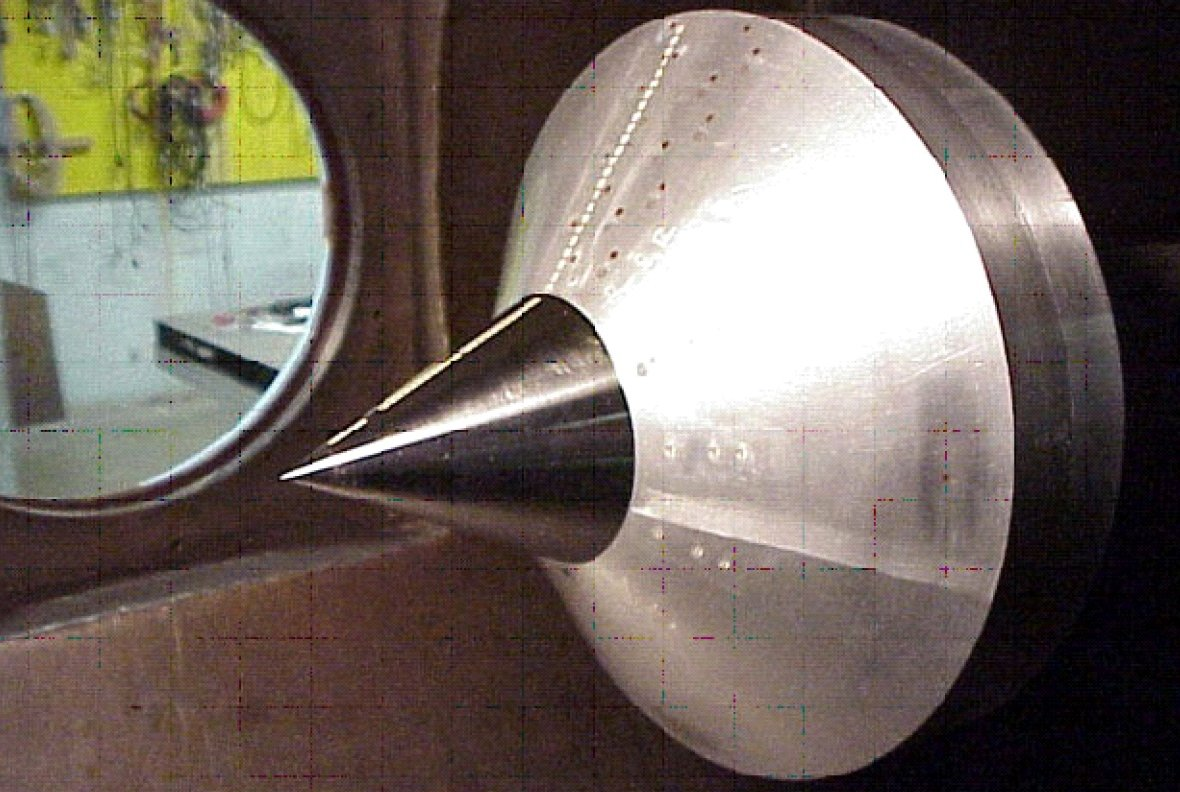
\includegraphics[width=\textwidth]{figures/holden_double_cone/test_article}} \\
    \subfigure[Schematic.  Dimensions are inches (millimeters).]{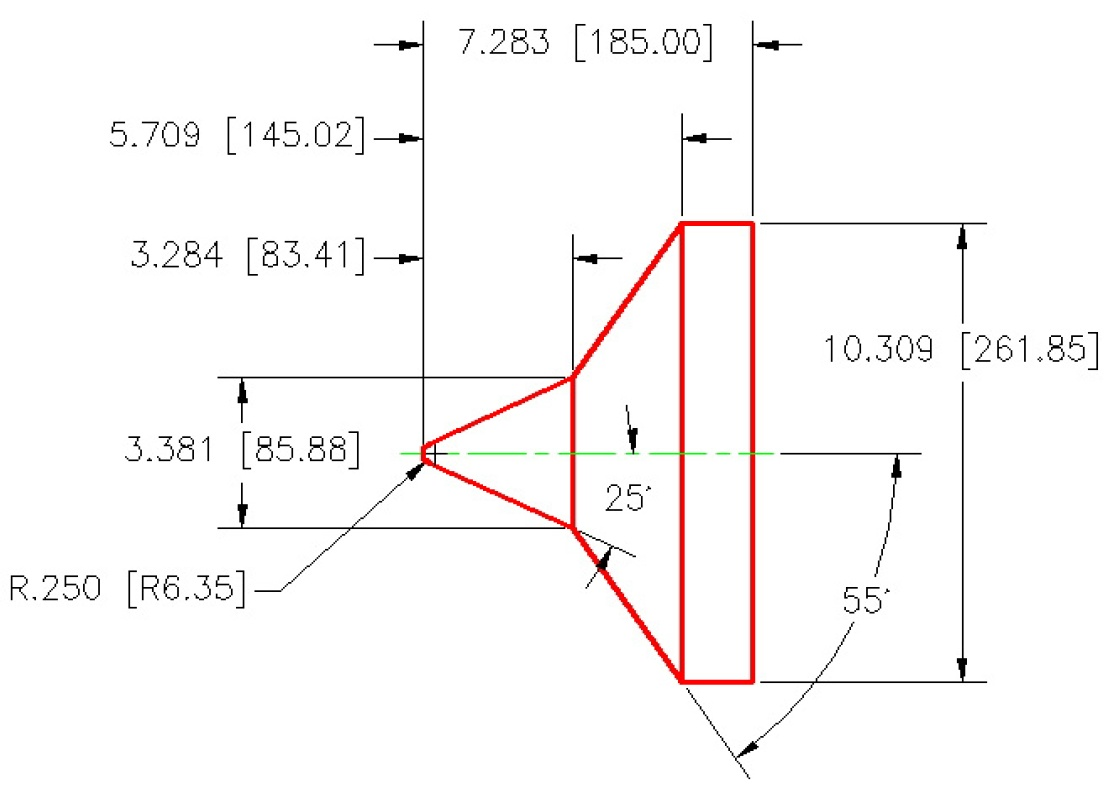
\includegraphics[width=.475\textwidth]{figures/holden_double_cone/schem_dimensions}}
    \subfigure[Instrumentation Layout.]{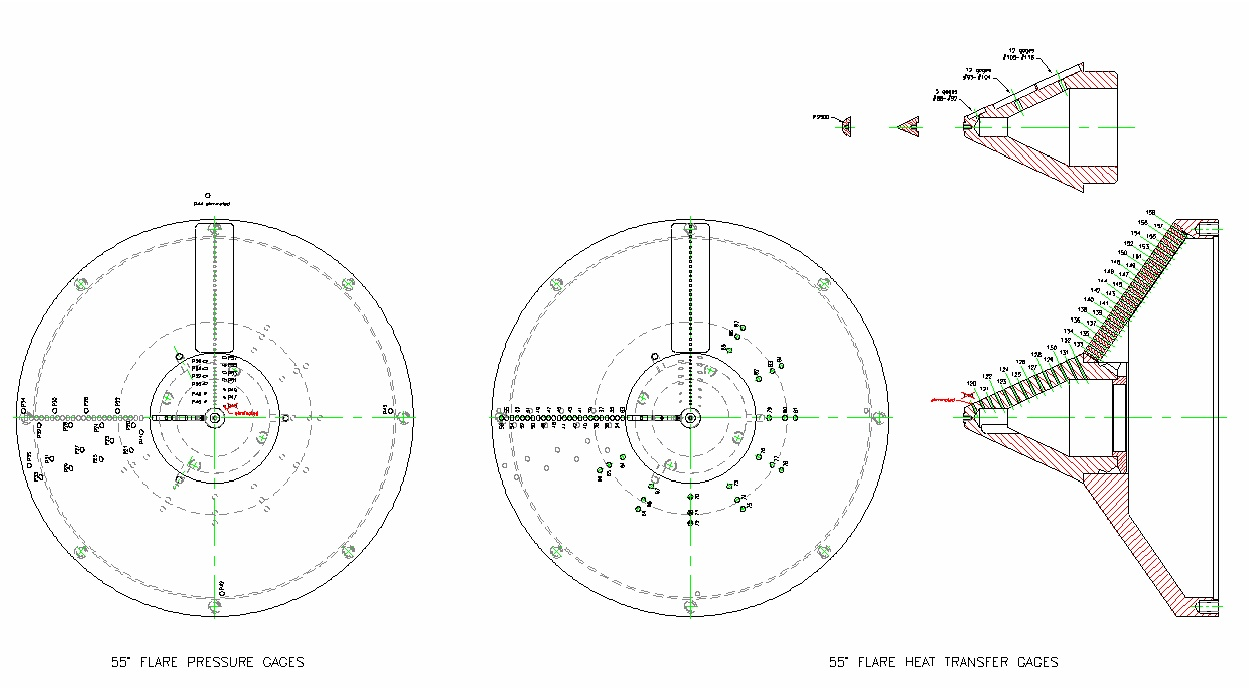
\includegraphics[width=.475\textwidth]{figures/holden_double_cone/instrumentation}}
    \caption[Double cone test article and dimensions.]{Double cone test article and dimensions~\cite{holden_wadhams_AIAA-2003-1137,maclean_AIAA-2004-529}.\label{fig:holden_double_cone_article}}
  \end{center}
\end{figure}

% Holden blunt double cone - freestream parameters
\begin{table}[hbtp]
  \begin{center}
    \caption[Freestream parameters for hypersonic blunt double cone benchmark.]{Freestream parameters for hypersonic blunt double cone benchmark~\cite{maclean_AIAA-2004-529}.\label{table:double_cone-freestream-parameters}}
    \vspace{1em}
    \begin{tabular}{cccc} \hline \hline
      M$_\infty$ & Re$_D$  & T$_\infty$ & T$_w$     \\
      12.43      & 53,666 & \unit[107]{K}   & \unit[297]{K} \\ \hline
    \end{tabular}
  \end{center}
\end{table}



\begin{figure}[hbtp]
  \begin{center}
    \subfigure[nondimensional static temperature.\label{fig:holden_double_cone_T}]{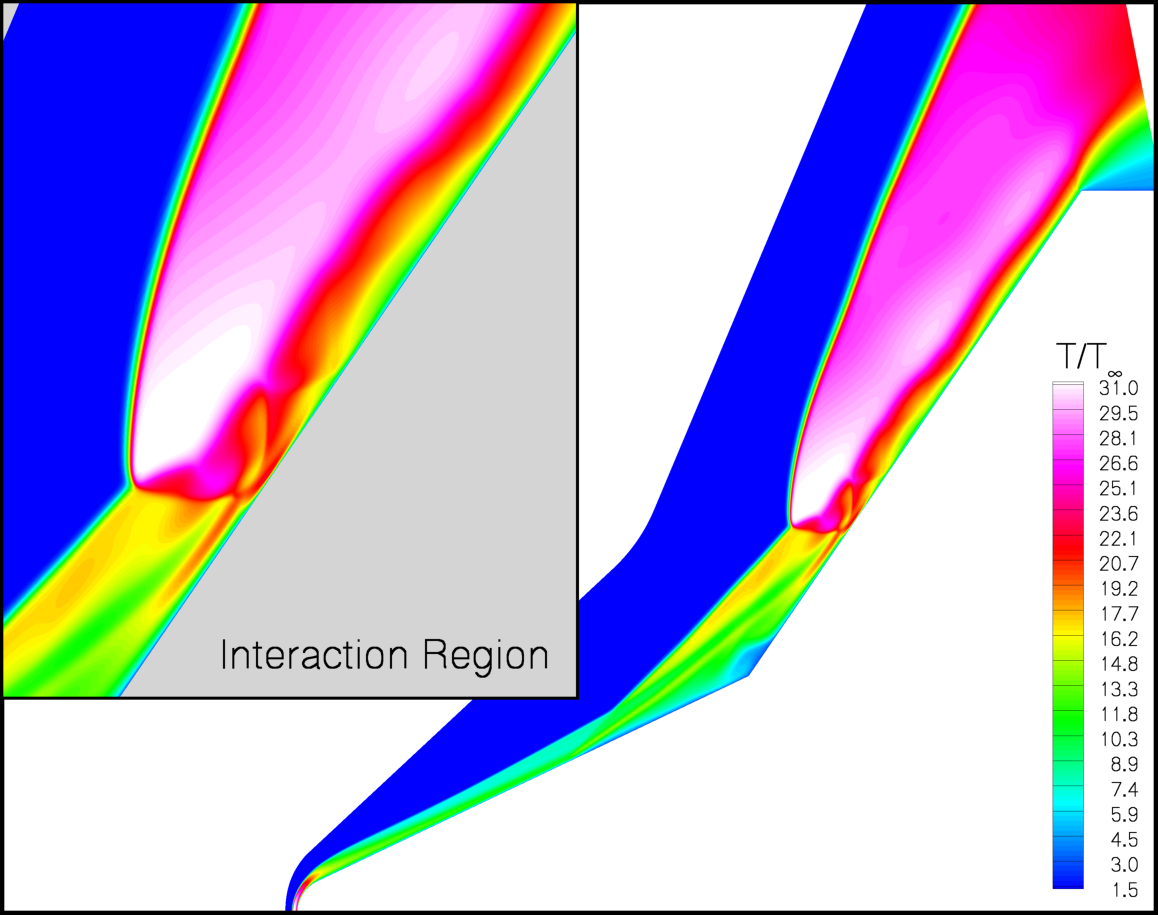
\includegraphics[width=0.48\textwidth]{figures/holden_double_cone/T}}
    \subfigure[nondimensional static pressure.\label{fig:holden_double_cone_P}]{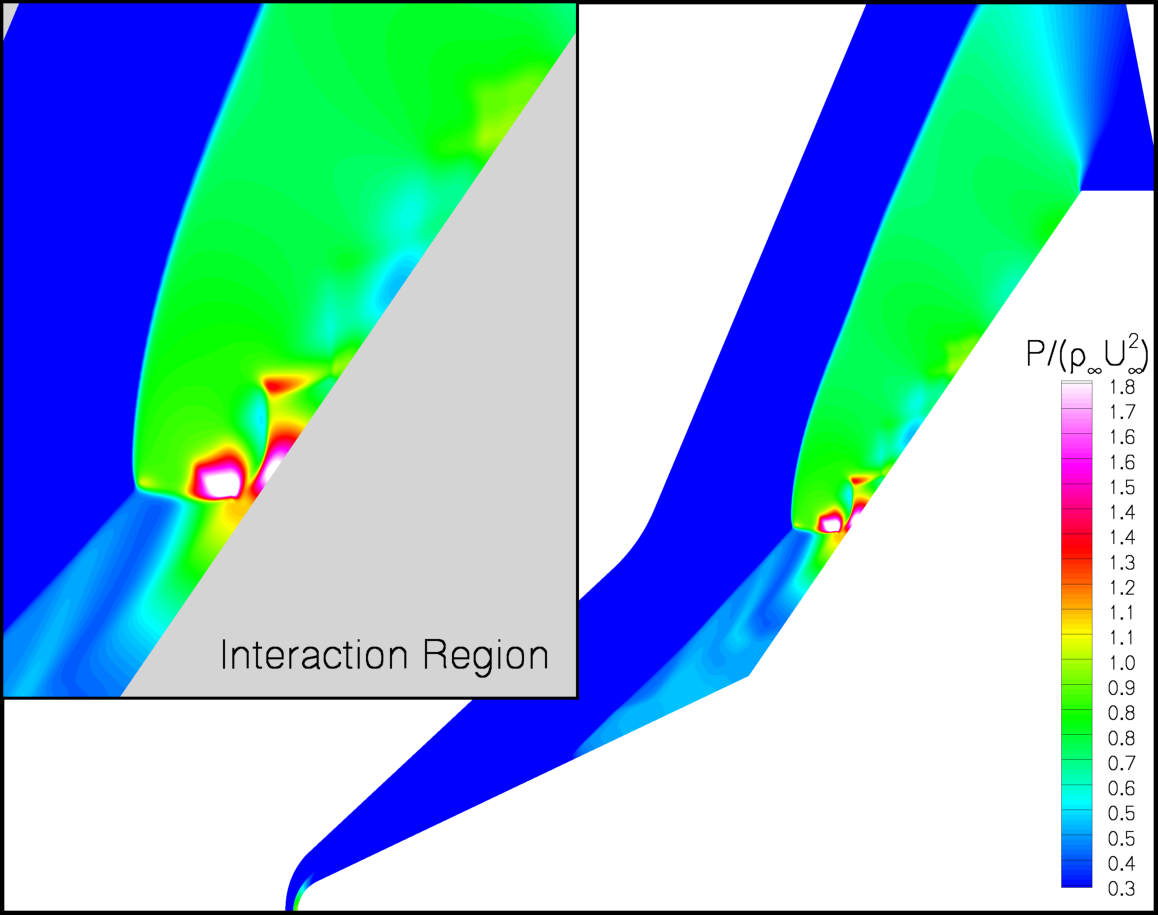
\includegraphics[width=0.48\textwidth]{figures/holden_double_cone/P}} \\
    \subfigure[Mach number.\label{fig:holden_double_cone_M}]{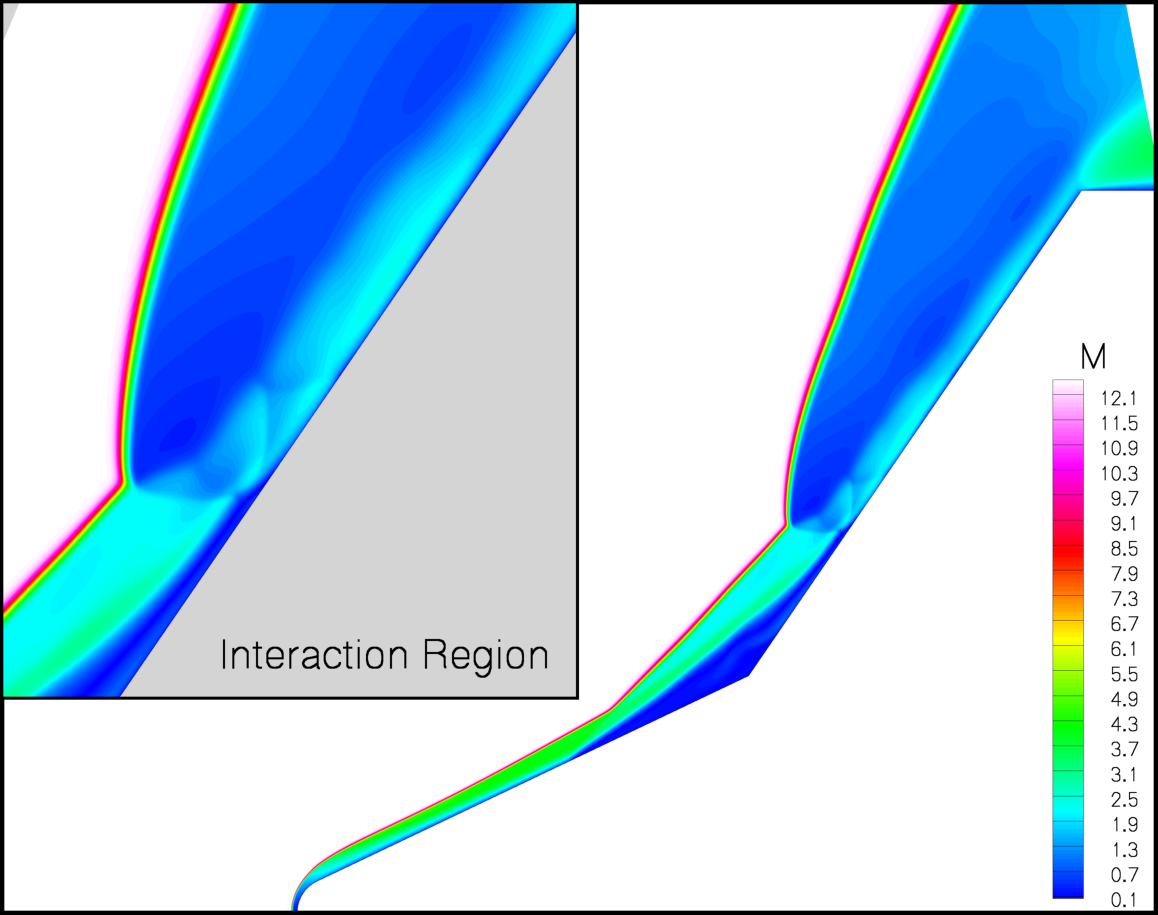
\includegraphics[width=0.48\textwidth]{figures/holden_double_cone/M}}
    \subfigure[computed schlieren.\label{fig:double_cone_schlieren}]{\includegraphics[width=0.48\textwidth]{figures/holden_double_cone/schlieren}}
    \caption{Illustration of flowfield for hypersonic blunt double cone shock interaction.\label{fig:holden_double_cone}}
  \end{center}
\end{figure}

%% \begin{figure}[hbtp]
%%   \begin{center}
%%     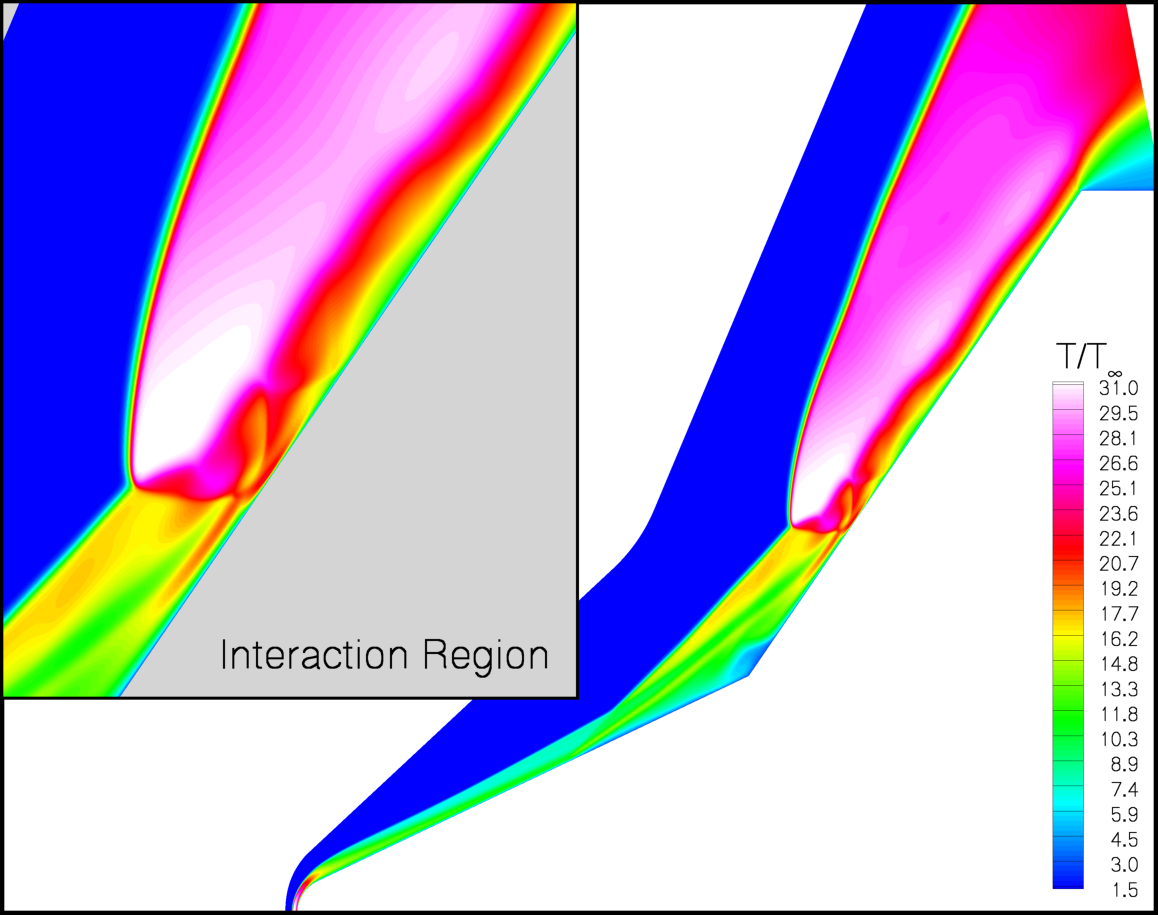
\includegraphics[width=\textwidth]{figures/holden_double_cone/T}
%%     \caption{Illustration of flowfield for hypersonic blunt double cone shock interaction problem: nondimensional static temperature.\label{fig:holden_double_cone_T}}
%%   \end{center}
%% \end{figure}

%% \begin{figure}[hbtp]
%%   \begin{center}
%%     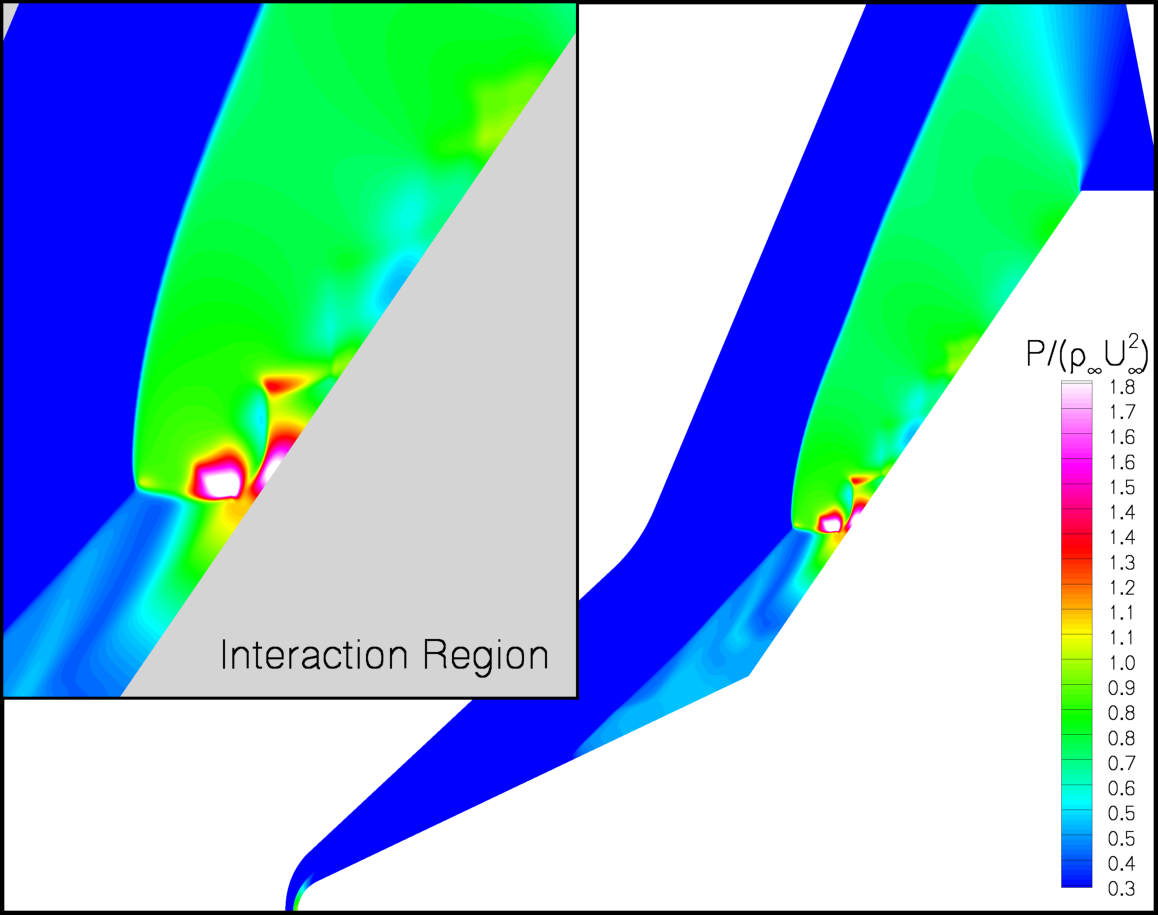
\includegraphics[width=\textwidth]{figures/holden_double_cone/P}
%%     \caption{Illustration of flowfield for hypersonic blunt double cone shock interaction problem: nondimensional static pressure.\label{fig:holden_double_cone_P}}
%%   \end{center}
%% \end{figure}

%% \begin{figure}[hbtp]
%%   \begin{center}
%%     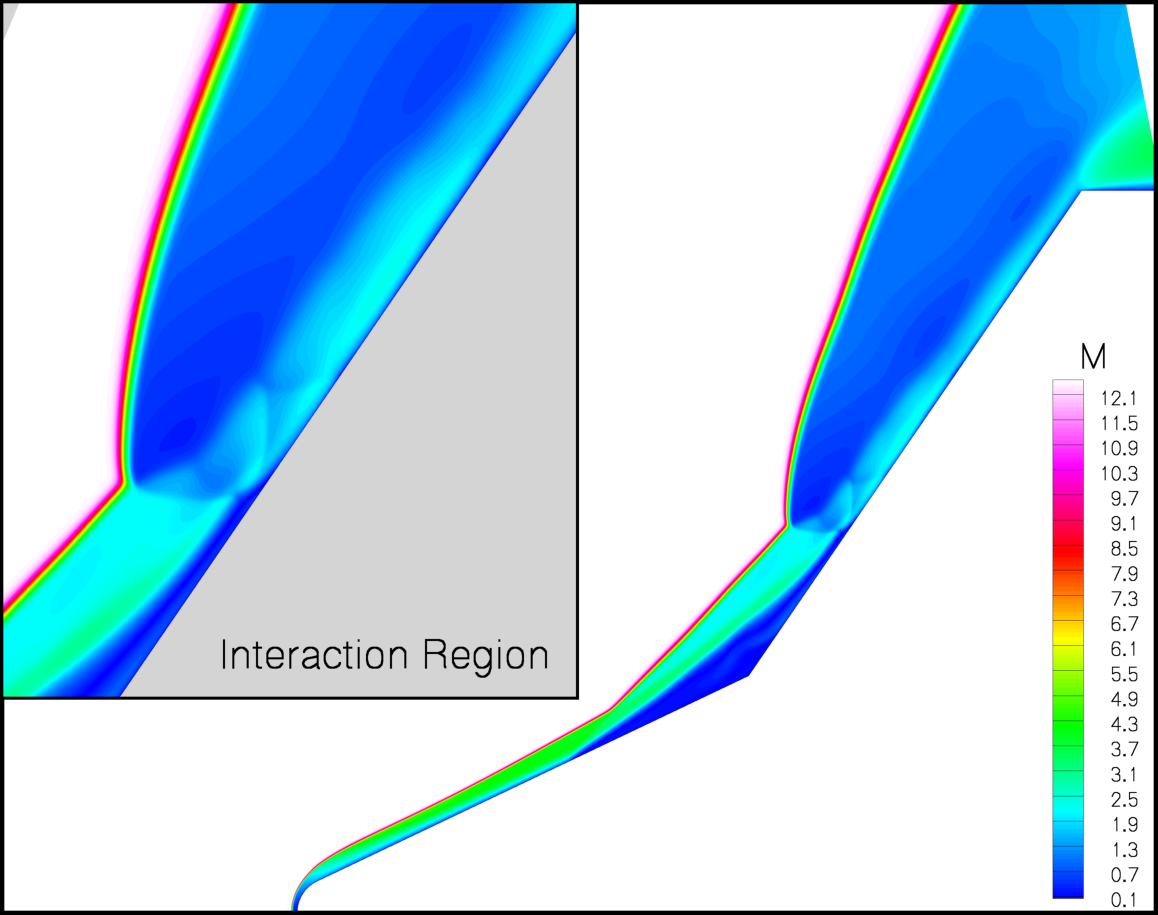
\includegraphics[width=\textwidth]{figures/holden_double_cone/M}
%%     \caption{Illustration of flowfield for hypersonic blunt double cone shock interaction problem: Mach number.\label{fig:holden_double_cone_M}}
%%   \end{center}
%% \end{figure}

Figure~\ref{fig:double_cone_schlieren} shows a computed schlieren image for the aforementioned case and depicts details of the complex shock interaction structure.  The image was generated by plotting the magnitude of the density gradient with a gray-scale color map.  As in schlieren photography, strong shock waves create a relatively larger density gradient and appear darker in the image.  This is particularly the case in the interaction region, where a nearly normal is shock set up by the $55^\circ$ cone.  The strength of this shock decreases away from the interaction region as it becomes increasingly oblique.

%% \begin{figure}[hbtp]
%%   \begin{center}
%%     \includegraphics[width=\textwidth]{figures/holden_double_cone/schlieren}
%%     \caption{Computed schlieren image for cone/cone shock interaction.\label{fig:double_cone_schlieren}}
%%   \end{center}  
%% \end{figure}


The oblique shock set up by the recirculation region is clearly evident in the figure.  This shock overtakes the weak attached shock produced by the $25^\circ$ forebody and interacts with the detached shock set up by the $55^\circ$ afterbody.  The shock interaction creates a transmitted shock which impacts the model surface, causing a local peak in surface pressure and heat transfer.

The image clearly illustrates the viscous slip surface emanating from the interaction region.  This forms a shear layer which separates two distinct regions of flow.  Above this feature the flow is subsonic, below it is supersonic.  This layer forms the boundary for the complex wave reflection pattern which is observed downstream of the interaction.  The transmitted shock reflects from the solid surface as a shock, which is then reflected from the shear layer as an expansion.  This pattern continues for several cycles downstream -- waves reflecting from solid surfaces as the same type and from the slip surface as opposite type.     


Figure~\ref{fig:double_cone_ch_cp} compares the measured and computed surface pressure and heat transfer for this case.  Immediately obvious is the large peak in surface pressure and heat transfer caused by the transmitted shock reflecting from the model surface.  
\begin{figure}[hbtp]
  \begin{center}
    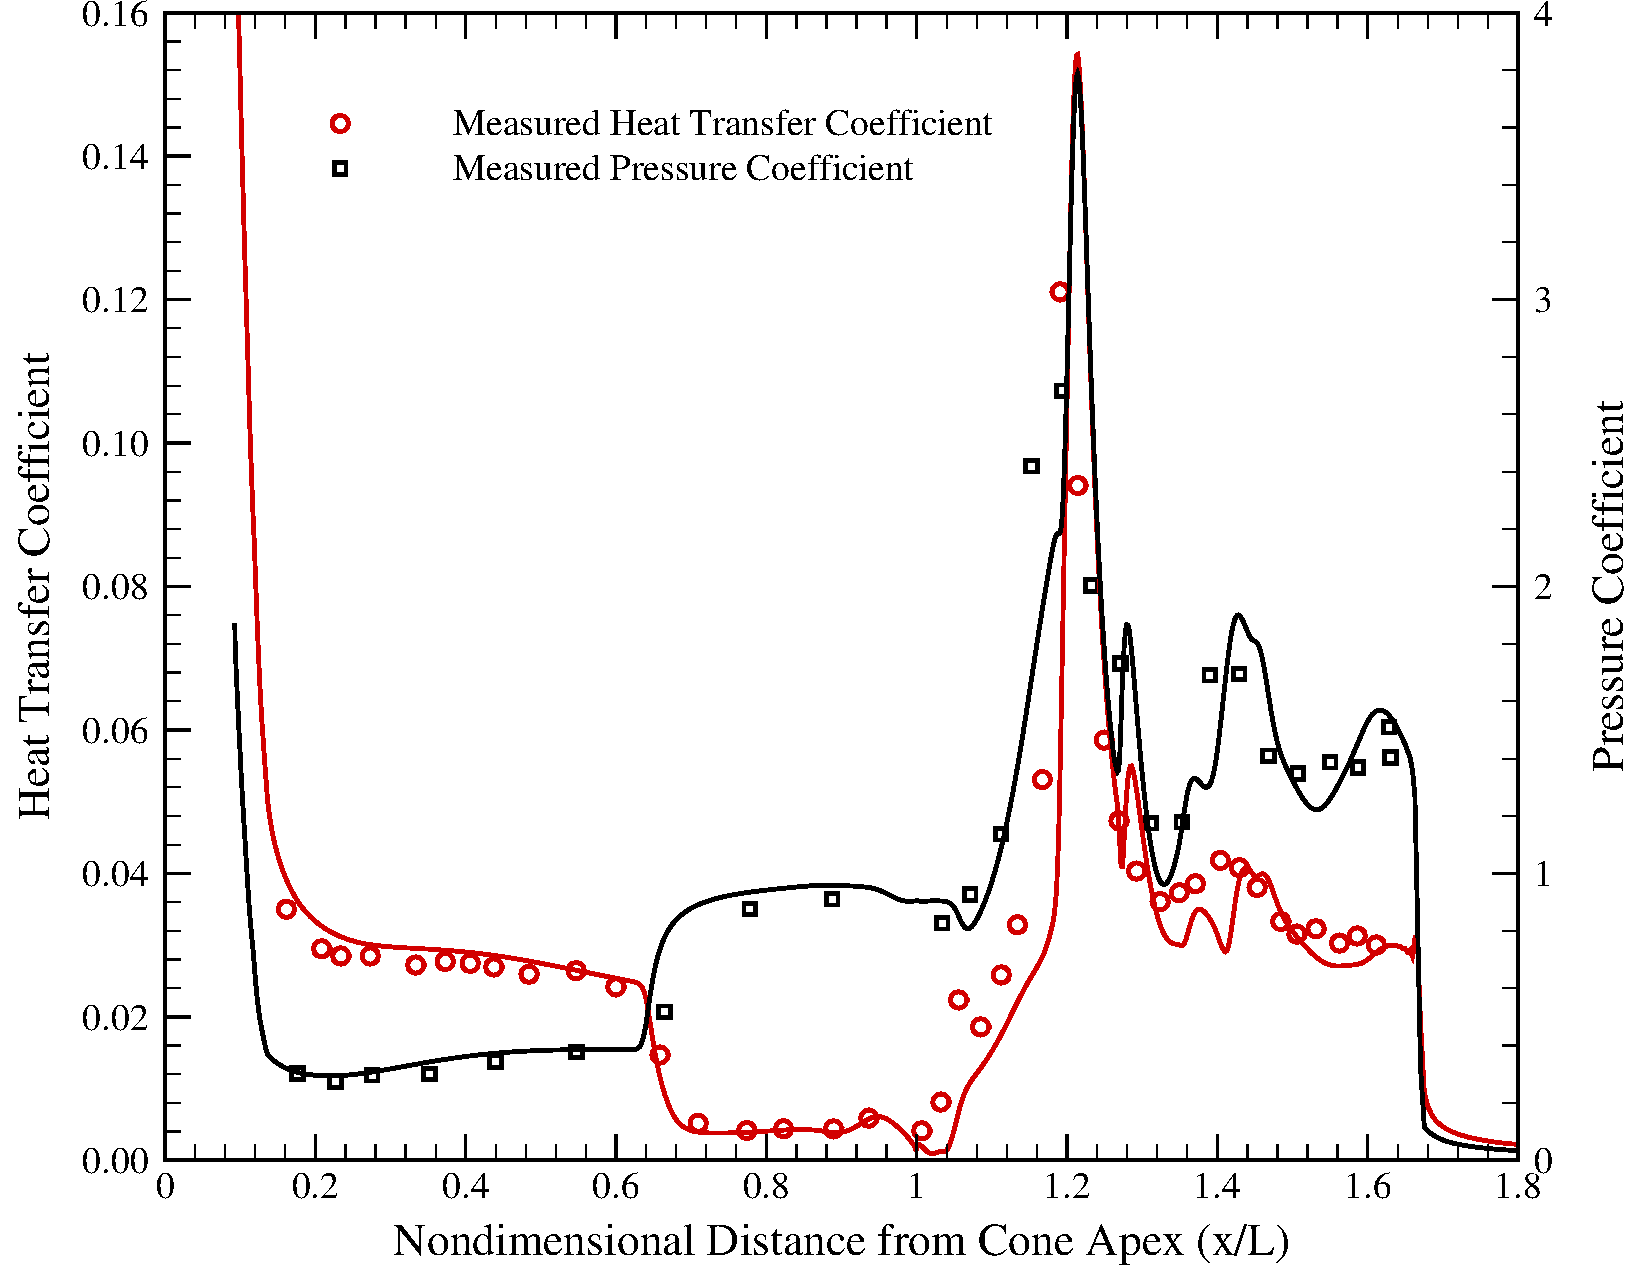
\includegraphics[width=\textwidth]{figures/holden_double_cone/ch_cp_comparison}
    \caption[Comparison of measured and computed heat transfer and pressure coefficients for cone/cone shock interaction.]{Comparison of measured and computed heat transfer and pressure coefficients for cone/cone shock interaction.\label{fig:double_cone_ch_cp}}
  \end{center}  
\end{figure}
Additionally, multiple secondary peaks in surface properties are visible on the afterbody region due to the complex wave reflection discussed previously.  It is interesting that the heat transfer and pressure on the forecone upstream of the separation point are not constant (as would be expected for a truly sharp cone).  This is in contrast to the sharp cone results which will be considered subsequently.  The variations in these properties are due to the phenomenon of ``entropy swallowing,'' which occurs when separate streamlines ingested by the boundary layer contain different entropy.  The presence of the blunt nose tip and corresponding curved shock structure induces this behavior.


\clearpage
\subsubsection{AEDC Sharp Double Cone}
As mentioned previously, the data obtained at AEDC Hypervelocity Wind Tunnel No.~9 and subsequent numerical investigations indicated the effect of vibrational nonequilibrium was negligible. However, these data exhibited considerable unsteadiness for all Reynolds numbers tested.  At high Reynolds numbers this behavior is to be expected as the flow will naturally transition from laminar to turbulent, but the observation of unsteadiness for purely laminar flows was unexpected in light of the CUBRC results.  Figure~\ref{fig:double_cone_in_tunnel_AEDC} shows the double cone (with the sharp nose tip) installed in the test section of HVWT9.
\begin{figure}[hbtp]
  \begin{center}
    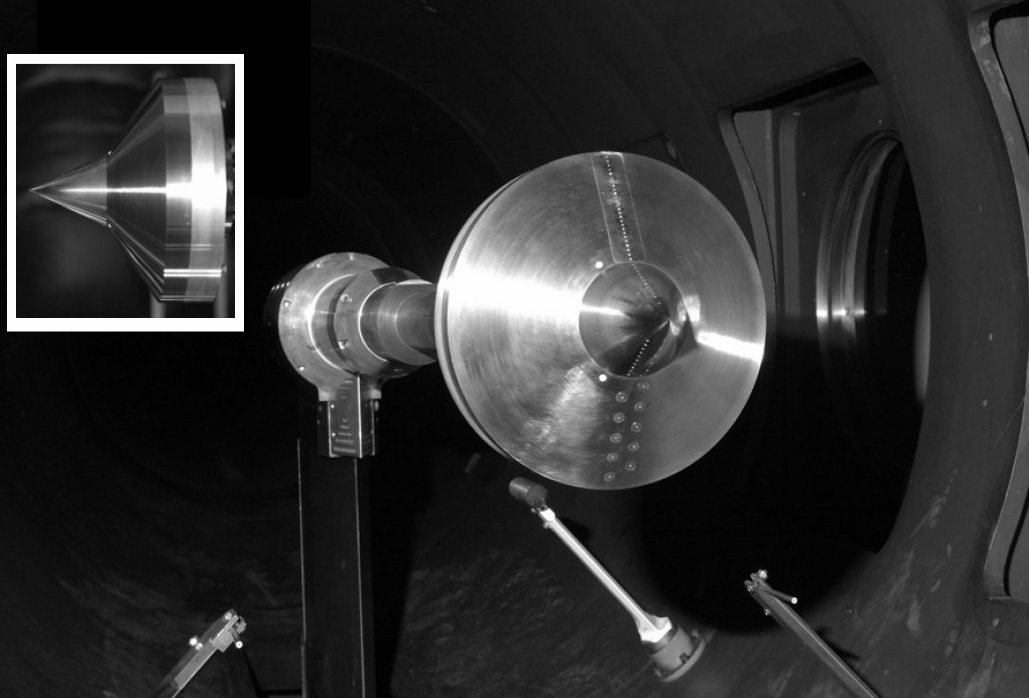
\includegraphics[width=\textwidth]{figures/aedc_double_cone/double_cone_HVWT9}
    \caption[Sharp double cone installed in the AEDC Hypervelocity Wind Tunnel No.~9]{Sharp double cone installed in the AEDC Hypervelocity Wind Tunnel No.~9~\cite{AEDC_HVWT9_double_cone}\label{fig:double_cone_in_tunnel_AEDC}}
  \end{center}
\end{figure}

The heat transfer and pressure gages are visible on the upper and lower surface of the model, respectively.
During the test series surface pressure and heat transfer data were collected and high-speed schlieren video were acquired.  Unfortunately, a light source failure prevented the investigators from obtaining high-speed schlieren for all runs.  Surface data were acquired for all runs and were observed to be unsteady.  Previous comparisons to computational simulations for fixed freestream conditions showed a substantial discrepancy between the data and the predictions~\cite{AEDC_HVWT9_double_cone}.


In this section laminar, calorically perfect Nitrogen flow over the sharp double cone model is examined for all Reynolds numbers tested.  First, simulations are conducted with a constant, uniform freestream to determine if the computation predicts a steady-state flowfield.  The response of the flowfield to freestream noise is then examined in detail in an attempt to explain the experimentally observed unsteadiness. 

  
\paragraph{Existence of a steady-state}

 Numerical simulations for the tested conditions were performed assuming a uniform, steady inflow profile based on conditions measured in the facility test section. Even for these steady input profiles, a stable steady-state solution to the Navier--Stokes equations may not exist.  This is especially the case for high Reynolds number flows or flows about complex geometries.  Time--accurate simulations were performed for all four test conditions assuming fixed, uniform inflow conditions given by the values listed in Table~\ref{table:double_cone_AEDC_freestream}.
\begin{table}[hbtp]
  \begin{center}
    \caption[AEDC Hypervelocity Wind Tunnel No.~9 sharp double cone freestream conditions.]{AEDC Hypervelocity Wind Tunnel No.~9 sharp double cone freestream conditions~\cite{AEDC_HVWT9_double_cone}.\label{table:double_cone_AEDC_freestream}}
    \vspace{1em}
    \begin{tabular}{|l||ccccl|}\hline
      Run             & 2890 & 2891  & 2893  & 2894  & \\ \hline\hline
      &      &       &       &       & \\
      M$_\infty$      & 13.6 & 13.17 & 12.73 & 12.63 & \\
      &      &       &       &       & \\
      Re$_{\text{D}}$ & $1.12\times 10^{6}$ &  $4.11\times 10^{5}$ & $8.44\times 10^{4}$ & $5.86\times 10^{4}$ & \\
      &      &       &       &       & \\
      $\rho_\infty$      & 7.81$\times 10^{-3}$     & 2.96$\times 10^{-3}$     & 5.90$\times 10^{-4}$       & 3.98$\times 10^{-4}$     &   $\unitfrac{kg}{m^3}$ \\
      &      &       &       &       & \\
      U$_\infty$      & 2006.6 & 1949.8 &  1763.5      & 1682.6     &   \unitfrac{m}{sec} \\
      &      &       &       &       & \\
      T$_\infty$      & 52.3 & 52.7 & 46.1   & 42.7 & \unit{K} \\ \hline
    \end{tabular}
  \end{center}
\end{table}
 It is important that the transient behavior of the flow be modeled accurately, because errors in time may mask the instability of an apparently steady flowfield.  In all cases the computational domain was initialized to freestream everywhere and marched in time until either steady-state was achieved or oscillatory behavior was evident.

\subparagraph{Runs 2893 and 2894}

Using this solution procedure steady-state solutions were obtained for the two lowest Reynolds numbers (runs 2893 and 2894) from the test series.  A computed schlieren image for both of these conditions is shown in Figure~\ref{fig:double_cone_AEDC_steady_schlieren}.
\begin{figure}[hbtp]
  \begin{center}
    %\subfigure[run 2894]{\includegraphics[width=.45\textwidth]{figures/aedc_double_cone/2894/schlieren}} \\
    %\subfigure[run 2893]{\includegraphics[width=.45\textwidth]{figures/aedc_double_cone/2893/schlieren}}
    \includegraphics[height=.875\textheight]{figures/aedc_double_cone/2893_2894_composite_schlieren}
    \caption{Sharp double cone steady-state computed schlieren images for the two lowest Reynolds numbers tested at AEDC Hypervelocity Wind Tunnel No.~9\label{fig:double_cone_AEDC_steady_schlieren}}
  \end{center}
\end{figure}
The primary features of the double cone flowfield discussed previously are present for these two cases: a large separated region, a separation shock, and separation shock/aftcone bow shock interaction.  Further, the extent of the separated region increases with increasing Reynolds number, as does the width of the compression/expansion reflection layer on the aftcone. With the increase in separated flow size, the strength of recirculation in this region increases, as illustrated by the streamlines plotted along with static temperature in Figure~\ref{fig:double_cone_AEDC_steady_streamlines}.
\begin{figure}[hbtp]
  \begin{center}
    \includegraphics[height=.875\textheight]{figures/aedc_double_cone/2893_2894_composite_streamlines}
    \caption{Sharp double cone steady-state static temperature and streamlines for the two lowest Reynolds numbers tested at AEDC Hypervelocity Wind Tunnel No.~9\label{fig:double_cone_AEDC_steady_streamlines}}
  \end{center}
\end{figure}

It is clear from this figure that at the lowest Reynolds number tested, Re$_\text{D}=58,600$, the separated region is dominated by one large recirculation zone with a significantly smaller reversed flow region at the $25^\circ/55^\circ$ cone junction. This small recirculation grows substantially as the Reynolds number is increased to Re$_\text{D}=84,400$, as shown in the bottom half of the figure.  This corner flow now has a pronounced effect on the primary recirculation region, essentially ``pinching'' it against the separation shock.  The end result is that for the higher Reynolds number case the extent of the separated region and strength of the shock-interaction induced shear layer are both increased. These flow structures are important because it will be shown that, for the case of uniform inflow, it is the interaction of these structures which drives the unsteadiness in the flowfield.

As discussed previously, the two steady-state solutions were obtained by solving the time--accurate Navier--Stokes equations until the time derivative term became negligible.  That is, the flow was initialized from freestream values and advanced in a time accurate fashion until $\left|\pdv{\bv{U}}{t}\right| \rightarrow 0$.  It is important that the time--accurate discretization be used in this case so that any natural unsteadiness in the flow will be captured accurately and not damped by an overly--dissipative time integration scheme.  This approach is in contrast to a typical local time step scheme in which the solution is assumed to be steady a priori, and the integration scheme advances each unknown in the discrete system by some maximum stable time step.  The local time step scheme is therefore clearly not time-consistent. This approach is often used to accelerate solution convergence in semi-implicit methods which have some upper bound on the stable time step.  This is the case, for example, in the familiar alternating--direction--implicit (ADI) or, to a lesser extent, line relaxation schemes.  By contrast, the stability afforded by the fully implicit formulation used in this work allows the solution to be advanced with globally large time steps in a time-consistent fashion.  

Figure~\ref{fig:aedc_double_cone_2894_time_convergence} shows the magnitude of the time derivative and the time step size as a function of time step number for run 2894 for a sequence of two meshes (similar results were obtained for run 2893 and are thus omitted).
\begin{figure}[hbtp]
  \begin{center}
    \includegraphics[width=\textwidth]{figures/aedc_double_cone/2894/resid_history}
    \caption{Sharp double cone time convergence for run~2894\label{fig:aedc_double_cone_2894_time_convergence}}
  \end{center}
\end{figure}
It is interesting that the fully implicit finite element discretization, initialized to freestream values, converges to a steady-state in approximately 250 time steps.  This result is especially promising given that the solution is time--accurate and does not resort to an inconsistent time discretization in order to accelerate convergence.  The plateau which occurs between time steps 25 and 125 corresponds to the initial development and subsequent growth of the recirculation region.  During this time the flow is changing appreciably because as the recirculation grows the separation shock moves, and in turn the shock interaction region moves.  


The driving mechanism in this flowfield is the boundary layer separation which occurs due to the adverse pressure gradient induced at the $25^\circ/55^\circ$ cone junction.  The separation region then produces an oblique shock which then impinges on the bow shock created by the aftcone.  Given this behavior, obtaining the proper separation point is crucial for simulating the flowfield accurately. To assess mesh convergence, the simulation was performed on a uniformly refined mesh (finer by a factor of four) for run 2894. The baseline and fine mesh solutions are compared in Figures~\ref{fig:aedc_double_cone_2894_mesh_convergence_P} and~\ref{fig:aedc_double_cone_2894_mesh_convergence_T} with overlaid static pressure and temperature contours, respectively.
\begin{figure}[hbtp]
  \begin{center}
    \subfigure[global flowfield]{\includegraphics[width=.68\textwidth]{figures/aedc_double_cone/2894/P_comp}} \\      
    \subfigure[interaction region]{\includegraphics[angle=270,width=.68\textwidth]{figures/aedc_double_cone/2894/P_comp_zoom}}
    \caption{Sharp double cone -- static pressure mesh convergence\label{fig:aedc_double_cone_2894_mesh_convergence_P}}
  \end{center}
\end{figure}

\begin{figure}[hbtp]
  \begin{center}
    \subfigure[global flowfield]{\includegraphics[width=.68\textwidth]{figures/aedc_double_cone/2894/T_comp}} \\      
    \subfigure[interaction region]{\includegraphics[angle=270,width=.68\textwidth]{figures/aedc_double_cone/2894/T_comp_zoom}}
    \caption{Sharp double cone -- static temperature mesh convergence\label{fig:aedc_double_cone_2894_mesh_convergence_T}}
  \end{center}
\end{figure}
In general, there is good agreement between the two solutions. The separation, shock interaction, and surface reflection are all captured well. As expected, the shock wave thickness scales with the local mesh size, so the shocks on the uniformly refined mesh are essentially half the width of those on the baseline mesh.  It is interesting that the \emph{post} shock location is nearly identical for the two solutions, and it is the shock foot that moves with mesh refinement.  This reinforces the observations of Section~\ref{sec:comp_ns_cyl}.




\clearpage
\subparagraph{Runs 2890 and 2891} 
The same solution procedure was applied to Re$_\text{D}=411,000$ and 1,120,000, the two highest Reynolds numbers in the test series.  A single frame taken from the high-speed schlieren video acquired during run 2890 is shown in Figure~\ref{fig:double_cone_exp_schlieren}.
Given the Reynolds number trend illustrated previously in Figure~\ref{fig:double_cone_AEDC_steady_streamlines}, it was expected that the extent of separated flow would be substantially larger and exhibit stronger rotation for these two cases.  Indeed, this was found to be the case.  For both conditions the separated region contains multiple, counter-rotating vortices which are highly dynamic.  This is the case even for a uniform, fixed inflow boundary condition, suggesting that there is no stable, laminar, steady solution to the governing equations for these conditions.  While the present work considers an axisymmetric flowfield, it is recognized that the resulting highly dynamic unsteadiness would likely be three-dimensional, even if it were possible to align the model perfectly with a uniform freestream and fix it entirely still. In reality, none of these conditions are possible to meet -- the freestream will always contain some nonuniformity, the model cannot be aligned perfectly, and model vibration is present (especially at high Reynolds number and corresponding high freestream dynamic pressure).       
\begin{figure}[hbtp]
  \begin{center}
    \includegraphics[width=\textwidth]{figures/aedc_double_cone/exp_schlieren_2892}
    \caption{Sharp double cone -- experimental schlieren image for run 2890.\label{fig:double_cone_exp_schlieren}}
  \end{center}
\end{figure}


Figure~\ref{fig:double_cone_AEDC_2891_unsteady} depicts the instantaneous flow about the model at four points in time for the case of Re$_\text{D}=411,000$.  Clearly, the size and structure of separated flow is highly dynamic and has a strong influence on the resulting downstream shock interaction.  Similar behavior was observed for Re$_\text{D}=1,120,000$ (albeit with a stronger shear layer instability) and is shown in Figure~\ref{fig:double_cone_AEDC_2890_unsteady}.  
\begin{figure}[hbtp]
  \begin{center}
    \includegraphics[width=0.94\textwidth]{figures/aedc_double_cone/2891/composite}
    \caption{Sharp double cone -- computed schlieren snapshots at four points in time for run 2891\label{fig:double_cone_AEDC_2891_unsteady}}
  \end{center}
\end{figure}
\begin{figure}[hbtp]
  \begin{center}
    \includegraphics[width=0.95\textwidth]{figures/aedc_double_cone/2890/composite}
    \caption{Sharp double cone -- computed schlieren snapshots at four points in time for run 2890\label{fig:double_cone_AEDC_2890_unsteady}}
  \end{center}
\end{figure}

For these two highest Reynolds numbers a Kelvin-Helmholtz instability develops in the shear layer emanating from the shock/shock interaction region.  Such an instability occurs when there is a velocity difference between two parallel flows.  In the inviscid limit such flows are inherently unstable, while viscous flows may be stabilized by the diffusion of vorticity in the viscous shear layer~\cite{viscous_shear_instabilities}. 

In summary, the present numerical method converged to a stable, steady, laminar flowfield for the two lowest Reynolds numbers tested.  The two highest Reynolds numbers, however, did not achieve a steady laminar state and contain large-scale dynamic shock/shock interaction even for the case of uniform inflow.  These numerical results are in contrast to the experimental data, which exhibited large scale unsteadiness for all Reynolds numbers tested.  The remainder of this section attempts to reconcile these differences first by assessing the impact of the variable model surface temperature on flowfield response and then by modeling the true unsteady freestream which occurs in all conventional wind tunnels.

%\clearpage
\paragraph{Steady state wall temperature sensitivity}  For all the cases presented previously the cone surface was modeled as a viscous isothermal wall at \unit[300]{K}.  One unique feature of the AEDC tunnel is that, as a blow-down tunnel, it has the ability to produce relatively long run times.  Runs in HVWT9 may be on the order of seconds, which is orders of magnitude higher than the order millisecond run times of shock-driven facilities.  For the lowest Reynolds number tested, run 2894, the run time was approximately 15 seconds.  During this time the model surface may heat up appreciably, especially in regions of localized heat transfer peaks.

The wall temperature variation during the course of a run is of concern because it is expected to have a direct impact on flowfield response.  For gases (whose viscosity increases with increasing temperature) wall cooling is known to have a stabilizing effect on the boundary layer.  Thus, for a cooler wall, the boundary layer should separate further downstream.  As the wall temperature increases, the boundary layer should become less stable and thus separate further upstream on the forecone due to the adverse pressure gradient induced by the base cone.  Of course, during the course of a run the model will heat up, so in order to quantify this effect in the context of the experimental investigation the simulation for the lowest Reynolds number was repeated for three different wall temperatures.  The wall temperature range of 300--\unit[400]{K} was chosen to bound the experimentally-measured model wall temperature as recorded by the surface thermocouples.

Figure~\ref{fig:double_cone_AEDC_2894_Twall} shows the results of this parametric study.
\begin{figure}[hbtp]
  \begin{center}
    \includegraphics[width=\textwidth]{figures/aedc_double_cone/2894/twall_Cp_comp}
    \caption{Influence of wall temperature on surface pressure distribution for run 2894.\label{fig:double_cone_AEDC_2894_Twall}}
  \end{center}
\end{figure}
As discussed previously, the decreasing stability with increasing wall temperature results in a larger separated region.  As a result, the overall size of the separated region is found to increase with increasing wall temperature as the upstream separation point moves forward and the downstream reattachment point moves aft.  From this study it is clear that, while the wall temperature does influence the size of the separated region, the effect is small for the temperature ranges which could be seen in a typical run.  Based on these analyses it is not believed that the experimentally observed unsteadiness is as a result of a temporal variation in the wall temperature.


\paragraph{Potential source of unsteadiness\label{sec:comp_ns_double_cone_unsteady}}

Conventional wind tunnels such as AEDC Hypervelocity Wind Tunnel No.~9 are known to contain freestream ``noise,'' which may be induced from flow nonuniformities in the nozzle reservoir, freestream turbulence, or from the tunnel wall turbulent boundary layer.  In conventional facilities this noise may produce root-mean-squared pitot pressure fluctuations on the order of 1\%--5\%.  These fluctations may produce an unsteady flowfield for a configuration which would otherwise be steady.  The remainder of this section examines the freestream noise characteristics of Hypervelocity Wind Tunnel No.~9.  In particular, the conjecture that freestream noise is the driving mechanism for the experimentally-observed unsteady flow at the low Reynolds numbers is addressed.

A set of experiments were recently performed in Hypervelocity Wind Tunnel No.~9 specifically designed to characterize freestream noise by measuring pitot acoustic fluctuations.  Kulite XT-140 pressure transducers were used to make standard pitot and flush-mounted pitot-acoustic measurements.  The measurements provide spectral resolution up to \unit[25]{kHz}~\cite{lafferty_norris_AEDC_noise}.  The test results indicate that for all nozzles used in HVWT9 the freestream noise is on the order of 5\%  root-mean-squared pitot fluctuation and increases with decreasing Reynolds number.  A possible explanation for this trend is that for lower Reynolds numbers the turbulent nozzle boundary layer is thicker and therefore has a larger acoustic influence on the reduced test core.

The power spectral density of the measured fluctuations was also examined. The power spectral density describes how the power of the signal is distributed with respect to frequency.  The tunnel noise was found to be broad and the fluctuations were random with a normal distribution over the measured frequencies of 0--\unit[25]{kHz}~\cite{lafferty_norris_AEDC_noise}.

Although the measurements indicate that the freestream noise is broad and randomly distributed over 0--\unit[25]{kHz}, for simplicity it is modeled numerically in this work as a sinusoidal pressure/density fluctuation of a given root-mean-square amplitude at a specified frequency. Additionally, while the measured data were restricted to \unit[25]{kHz} temporal resolution, the fact that the noise is broad over the range captured suggests there are likely  higher frequency components as well, therefore the subsequent numerical experiments will include higher frequencies.  Both the freestream density and static pressure are chosen to vary in phase while all other freestream conditions are fixed.  Specifically, the applied perturbations are
\begin{equation}
  \left(P,\rho\right) = \left(\bar{P},\bar{\rho}\right)\left[1 + \sqrt{2}\Lambda\sin\left(2\pi\lambda t - \frac{x}{\text{U}_\infty}\right) \right]
\end{equation}
where $\Lambda$ is the root-mean-squared value of the noise perturbation, $\lambda$ is the specified frequency, and $\bar{()}$ denotes average values. It can be shown from normal shock relations that changes in freestream density and pressure are magnified appreciably through a shock wave; hence, perturbing these properties allows for substantial temporal variation in the flowfield.

Of particular interest is the stability of the shock interaction induced shear layer.  At the two highest Reynolds numbers tested, the shear layer was observed to develop a classic Kelvin-Helmholtz instability.  This type of instability results when there is a velocity difference between two adjacent layers of fluid.  In the inviscid limit, which is approached with increasing Reynolds number, the interface is unstable to all disturbance modes.  For finite width shear layers with appreciable vorticity diffusion via viscous forces, however, the interface is subject to the competing effects of diffusion and inviscid layer instability~\cite{viscous_shear_instabilities}.  It is hypothesized that, for the lower Reynolds numbers tested under the assumption of a uniform freestream, this is precisely the case -- that viscous diffusion mitigates the natural shear layer instability for the length scales present in the flowfield.  However, the question that remains is whether the shear layer instability (or any other instability, for that matter) will be excited by the freestream noise which is present in the facility.

%\subparagraph{Noise Frequency Sensitivity}

To analyze the receptivity of the simulation to freestream noise run 2894 was repeated for a range of disturbance frequencies, $\lambda$, assuming a representative root-mean-squared pitot pressure fluctuation of 6\%~\cite{lafferty_norris_AEDC_noise}. The simulation was initialized with the steady solution previously obtained for uniform inflow.  The mean surface pressure coefficient distributions for several specified frequencies are shown in Figure~\ref{fig:double_cone_AEDC_2894_unsteady_6percent_Cpavg_comp}.
\begin{figure}[hbtp]
  \begin{center}
    \includegraphics[width=.9\textwidth]{figures/aedc_double_cone/2894/Cp_freq_comp}
    \caption{Sharp double cone -- measured and computed surface pressure coefficient distribution for run 2894 with \unit{6.5--50}{kHz}, 6\%~RMS freestream noise.\label{fig:double_cone_AEDC_2894_unsteady_6percent_Cpavg_comp}}
  \end{center}
\end{figure}
The steady distribution is plotted as the thick black line. There is negligible influence of freestream noise at the two lower frequencies simulated as they produce essentially the same mean surface pressure distribution as the nominal, quiescent freestream case.  As the frequency is increased, however, the extent of the separated region is reduced, suggesting that the additional energy in the oscillating inflow helps delay separation.


Surface traces for these four frequencies are detailed in Figure~\ref{fig:double_cone_AEDC_2894_unsteady_6percent_Cpavg}.
The mean values for both the experimental data and the numerical simulation are computed, as is the standard deviation of the time history for each point.
\begin{figure}[hbtp]
  \begin{center}
    \subfigure[6.5 kHz]{\includegraphics[width=.48\textwidth]{figures/aedc_double_cone/2894/Cp_6kHz_6percent}}
    \subfigure[13 kHz]{\includegraphics[width=.48\textwidth]{figures/aedc_double_cone/2894/Cp_13kHz_6percent}} \\
    \subfigure[25 kHz]{\includegraphics[width=.48\textwidth]{figures/aedc_double_cone/2894/Cp_25kHz_6percent}}
    \subfigure[50 kHz]{\includegraphics[width=.48\textwidth]{figures/aedc_double_cone/2894/Cp_50kHz_6percent}}
    \caption{Sharp double cone -- measured and computed surface pressure coefficient distribution for run 2894 with 6\%~RMS freestream pitot pressure noise for a range of disturbance frequencies.\label{fig:double_cone_AEDC_2894_unsteady_6percent_Cpavg}}
  \end{center}
\end{figure}
The error bars plotted with the data correspond to $\pm 2\sigma$, which bound 95\% of the experimentally measured values.  The blue solid line corresponds to the average pressure coefficient extracted from the transient simulation.  Additionally, the two faint traces bounding the mean correspond to the $\pm 2\sigma$ temporal variation in the computed distributions.

The $\pm 2\sigma$ bounds in the figures illustrate how dynamic the surface interaction is for \emph{all} frequencies simulated.  Interestingly, even the lower frequencies exhibit a substantial  temporal variance even though the average distribution is not markedly different than for uniform inflow.  To illustrate the dynamic nature of the data Figure~\ref{fig:double_cone_AEDC_2894_unsteady_50kHz_6percent_Cptrace} shows instantaneous pressure traces plotted at several discrete times for the case of~\unit[50]{kHz} freestream noise. 
\begin{figure}[hbtp]
  \begin{center}
    \includegraphics[width=\textwidth]{figures/aedc_double_cone/2894/2894_50kHz_6RMS_Cptrace}
    \caption{Sharp double cone -- surface pressure coefficient distribution at several instances for run 2894 with \unit{50}{kHz}, 6\%~RMS freestream noise.\label{fig:double_cone_AEDC_2894_unsteady_50kHz_6percent_Cptrace}}
  \end{center}
\end{figure}


Figure~\ref{fig:double_cone_AEDC_2894_unsteady_6percent_St} shows the impact of these freestream fluctuations on the surface heat transfer.  Again, the temporal variation in both the data and the predictions are averaged and the standard deviation at each location is computed.
\begin{figure}[hbtp]
  \begin{center}
    \subfigure[25~kHz]{\includegraphics[height=.41\textheight]{figures/aedc_double_cone/2894/St_25kHz_6percent}} \\
    \subfigure[50~kHz]{\includegraphics[height=.41\textheight]{figures/aedc_double_cone/2894/St_50kHz_6percent}} 
    \caption{Sharp double cone -- measured and computed Stanton number distribution for run 2894, 6\%~RMS freestream noise.\label{fig:double_cone_AEDC_2894_unsteady_6percent_St}}
  \end{center}
\end{figure}


The general flowfield is imaged at four instances for the case of~\unit[50]{kHz} noise in Figure~\ref{fig:double_cone_AEDC_2894_unsteady_50kHz_6percent}.
\begin{figure}[hbtp]
  \begin{center}
    \includegraphics[width=\textwidth]{figures/aedc_double_cone/2894/2894_50kHz_6RMS}
    \caption{Sharp double cone -- computed schlieren snapshots at four points in time for run 2894 with \unit{50}{kHz}, 6\%~RMS freestream noise.\label{fig:double_cone_AEDC_2894_unsteady_50kHz_6percent}}
  \end{center}
\end{figure}
There are substantial differences in the structure of the separated region, shock interaction region, and aftcone wave reflection.


%\subparagraph{Noise Amplitude Sensitivity}

\clearpage
\paragraph{Observations}
The experimental data obtained in AEDC Hypervelocity Wind Tunnel No.~9 for four separate Reynolds numbers in the nominally Mach 14 nozzle exhibited large-scale unsteadiness as evident in both high-speed schlieren imagery and surface instrumentation.  Unfortunately, the surface gage response time was not adequate to resolve instantaneous heat transfer or pressure distributions, but average values were obtained over long run times.

It was verified for the two lowest Reynolds numbers tested that simulations assuming fixed, uniform inflow converged to steady-state.  For the two higher Reynolds numbers the flows were naturally unsteady, predominantly due to the Kelvin-Helmholtz instability in the shear layer emanating from the shock interaction region.
The hypothesis that freestream noise is the dominant mechanism for creating the unsteadiness at low Reynolds number was tested by subjecting the lowest Reynolds number case to freestream pitot pressure fluctuations which are representative of the fluctuations seen in HVWT9.  The average surface pressure and heat transfer obtained in the presence of freestream noise agree well with the data -- although it is difficult to make a conclusive observation due to the lack of temporal resolution in the surface instrumentation.  A more rigorous experimental investigation of the influence of freestream noise would be worthwhile and should include high-rate thermocouples or thin-film gages for high temporal resolution of these unsteady flow phenomena.

It is interesting to note that the primary surface response to the sinusoidal freestream perturbation is an in-phase amplitude oscillation of the computed surface quantities of interest.  Notably, there is little change in the streamwise location of both the peak heat flux and pressure.  Future work could consider unsteadiness in the case of a fully three-dimensional time accurate simulation to investigate the possibility of other unsteady modes which may be precluded by the assumption of axisymmetry.  Another possibility for future work is the modeling of the broadband noise present in the facility.  This approach will require additional data at various radial stations in the test section to help correlate possible spatial behavior in the noise.


%%%%%%%%%%%%%%%%%%%%%%%%%%%%%%%%%%%%%%%%%%%%%%%%%%%%%%%%%%%%%%%%%%%%%%%%%%%%%%%
\clearpage
\subsection{Transient Hypersonic Flow over a Nose Tip/Forward Facing Cavity Configuration}

In this section hypersonic flow over a missile nose tip with a forward facing cavity is investigated.  This configuration, shown schematically in Figure~\ref{fig:cavity_LD2_schematic}, has been observed to exhibit a transient flowfield response in both experimental investigations and numerical simulations~\cite{engblom_goldstein_AIAA-1996-667,engblom_goldstein_AIAA-1996-354,silton_goldstein_JTHPHT}.  The dynamics of the response are largely driven by the cavity length-to-diameter ratio (L/D).  Experimental studies in conventional tunnels report oscillatory response even for relatively shallow cavities, suggesting an unsteady threshold L/D of 0.4. Numerical simulations predict a higher threshold L/D of approximately 1.25 for transient response.
\begin{figure}[hbtp]
  \begin{center}
    \includegraphics[angle=270,width=\textwidth]{figures/sphere_cavity/LD_2.0/schematic}
    \caption{Schematic diagram of a forward facing cavity nose tip with a length-to-diameter ratio of 2\label{fig:cavity_LD2_schematic}}
  \end{center}
\end{figure}

\clearpage
Subsequent experiments in a quiet wind tunnel~\cite{engblom_goldstein_AIAA-1996-667} have shown threshold L/D ratios similar to those predicted by numerical experiments, indicating that freestream noise is the mechanism which drives unsteady response in the 0.4~$<$~L/D~$<$~1.25 range.  Subsequent numerical studies which model freestream noise have verified this observation.  Further, numerical studies with relatively deep cavities (L/D~$>$~1.5) exhibit unsteady response even for uniform inflow conditions~\cite{engblom_goldstein_AIAA-1996-354,silton_goldstein_JTHPHT}. 

The goal of the current analysis is to examine the accuracy and efficiency of the fully implicit finite element scheme for transient applications.  Of particular interest is the need to maximize the time step used in the simulation while maintaining time accuracy.  It is hypothesized that the fully implicit approach used in this work will admit substantially larger time steps than were possible with the numerical treatments used in previous studies. If this hypothesis is verified the result may reduce the computational time required to simulate a given number of flowfield response periods.

It should be noted that a detailed parametric study of model response for a range of cavity geometries and flow conditions is beyond the scope of this work. (A thorough parametric study was conducted in the experimental setting by Silton~\cite{silton_dissertation}.)  Rather, this example is chosen to test the current algorithm largely \emph{because} of the amount of previous work.  This allows the current work to focus on algorithmic details without probing the parametric space of cavity response or attempting to characterize the impact of freestream disturbances.

\subsubsection{Model Geometry and Flow Conditions}
The numerical simulation is chosen to replicate wind tunnel conditions studied by Silton and Goldstein in The University of Texas at Austin's Mach 5 blow-down facility located at the J.J.\ Pickle Research Campus.  In the experimental studies ice models were produced from molds and then cooled in liquid N$_2$ vapors to a uniform temperature of approximately \unit[78]{K}.  The models were then exposed to the Mach~5 stream and the time required for the onset of melting was recorded.  Previous work has focused on coupling the flow-induced heat flux with the solid body thermal response to predict melting onset time and comparing the predicted and measured values~\cite{silton_goldstein_JFM}.

The model simulated in this case is a spherically blunted cylinder with a nose tip cavity, similar to the notional geometry shown in Figure~\ref{fig:cavity_LD2_schematic}.  The spherical nose diameter, D$_N$, is \unit[2.54]{cm}, the cavity diameter D is \unit[1.031]{cm}, and the cavity length, L, is \unit[2.062]{cm}. The lip transition between the cavity wall and the spherical nose segment has a radius of \unit[0.119]{cm}.  The length-to-diameter ratio, L/D, is 2.0, which is sufficiently deep that unsteady motion is expected even for a uniform freestream.

The tunnel was operated at a nominal stagnation pressure, P$_0$, and temperature, T$_0$, of \unit[2.3]{MPa} and \unit[370]{K}, respectively.  The flow is expanded to a freestream Mach number of 4.91, resulting in a freestream unit Reynolds number of $\unitfrac[5\times 10^7]{1}{m}$.  This yields a Reynolds number based on model nose diameter, D$_N$, of Re$_N=1.2\times 10^6$.  The remaining freestream static properties of interest are presented in Table~\ref{table:cavity_LD2_freestream-parameters}.  The model wall temperature was fixed at \unit[130]{K}, while during the run the actual model temperature obviously varied from its initial value of approximately \unit[100]{K} to \unit[273]{K} (the model melt temperature of ice).
% J.J. Pickle Mach 5 test - freestream parameters
\begin{table}[hbtp]
  \begin{center}
    \caption[Freestream parameters for nose tip/forward facing cavity configuration.]{Freestream parameters for nose tip/forward facing cavity configuration.\label{table:cavity_LD2_freestream-parameters}}
    \vspace{1em}
    \begin{tabular}{cccc} \hline \hline
      M$_\infty$ & Re$_N$            & T$_\infty$    & T$_w$          \\
      4.92       & $1.27\times 10^6$ & \unit[64.]{K} & \unit[130.]{K} \\ \hline
    \end{tabular}
  \end{center}
\end{table}

\clearpage
\subsubsection{Computational Mesh}
A block-structured grid topology was used to discretize the domain, as shown in Figure~\ref{fig:cavity_mesh}. The outer boundary of the grid was positioned so as to contain the bow-shock at its farthest upstream location.  The off-body grid was created by using a hyperbolic marching technique from the model surface.  The primary features of the hyperbolic grid generation scheme used is that it attempts to preserve mesh orthogonality and maintain smooth size transition simultaneously~\cite{gridgen}.  The mesh contains a total of 28,544 quadrilateral elements with 28,949 nodes.
\begin{figure}[hbtp]
  \begin{center}
    \includegraphics[width=.85\textwidth]{figures/sphere_cavity/LD_2.0/grid}
    \caption[Computational mesh used for an L/D=2 cavity in a spherically blunted nose tip.]{Computational mesh used for an L/D=2 cavity in a spherically blunted nose tip.  (Every-other point is shown)\label{fig:cavity_mesh}}
  \end{center}
\end{figure}

\clearpage
The mesh was partitioned into 64 subdomains and run on the \emph{Columbia} supercomputer at NASA Ames Research Center.  The partitioned mesh, colored by subdomain, is shown in Figure~\ref{fig:cavity_mesh_partition}. The disparate physical sizes of the subdomains is due to the differences in local element size.  Each subdomain contains roughly the same number of elements in order to balance the computational load.
\begin{figure}[hbtp]
  \begin{center}
    \includegraphics[width=\textwidth]{figures/sphere_cavity/LD_2.0/partition}
    \caption{Computational mesh used for an L/D=2 cavity in a spherically blunted nose tip partitioned into~64 subdomains.\label{fig:cavity_mesh_partition}}
  \end{center}
\end{figure}

\clearpage
\subsubsection{Transient Solution Scheme}
The time step control strategy outlined in Section~\ref{sec:comp_ns_cyl} is modified somewhat here such that the Courant-Friedrichs-Lewy, or CFL, number is the controlled value.  The CFL number defines the ratio of characteristic flow length per time step to element size and is often used to describe the time step procedure used in semi-implicit techniques such as the aforementioned LU-SGS algorithm.  The CFL-based time step selection used during the simulation is as follows:
\begin{enumerate}
  \tightlist
  \item Compute the characteristic convection time step for each element as
    \begin{equation*}
      \Delta t_e = \frac{h^e_{min}}{\|\bv{u}\| + c}
    \end{equation*}
  \item Determine the global minimum characteristic time step
    \begin{equation*}
      \Delta t_{min} = \min(\Delta t_e)
    \end{equation*}
  \item Set the time step $\Delta t_{n+1} \equiv t_{n+1}-t_n$ for the simulation as a user-specified multiple of $\Delta t_{min}$
    \begin{equation}
      \Delta t_{n+1} = \mbox{CFL}_{n+1}\times \Delta t_{min}
    \end{equation}
    where CFL$_{n+1}$ is taken as
    \begin{equation}
      \mbox{CFL}_{n+1} = \min\left(\left(\eta^{n+1}\right)\mbox{CFL}_0, \mbox{CFL}_{\max}\right),\;\; \eta \ge 1,\; n=0,1,2,\ldots
      \label{eq:CFL_np1}
    \end{equation}
    where $\eta$ is a user-specified time step growth rate and CFL$_0$ is the initial time step factor, which is taken as CFL$_0$=200 in all cases presented in this section.
\end{enumerate}


\subsubsection{Fixed-Mesh Results}

Figure~\ref{fig:cavity_LD2_flowfield} shows the static pressure and temperature external to the model and within the cavity at the extreme outboard and inboard bow shock locations. This behavior is consistent with previous research by Engblom and Silton using the commercial CFD code INCA~\cite{engblom_goldstein_AIAA-1996-667,silton_goldstein_JFM}.
\begin{figure}[hbtp]
  \begin{center}
    \subfigure{\includegraphics[width=.43\textwidth]{figures/sphere_cavity/LD_2.0/P_in}}
    \subfigure{\includegraphics[width=.43\textwidth]{figures/sphere_cavity/LD_2.0/P_out}} \\
    \subfigure{\includegraphics[width=.43\textwidth]{figures/sphere_cavity/LD_2.0/T_in}}
    \subfigure{\includegraphics[width=.43\textwidth]{figures/sphere_cavity/LD_2.0/T_out}}
    \caption{Flowfield about a nose tip/forward facing cavity configuration.  Static pressure and temperature distribution for bow shock location extrema.\label{fig:cavity_LD2_flowfield}}
  \end{center}
\end{figure}
This cyclic bow shock motion was observed both experimentally and computationally to reduce the net heat transfer into the model.  An excellent summary of the fluid dynamic processes which cause this heat flux decrease are presented by Engblom and Goldstein in~\cite{engblom_goldstein_AIAA-1996-354} but merit discussion here as they aid in understanding the nature of the transient flow. 

A bow shock oscillation cycle in this problem can be divided into two distinct phases: movement toward the model, and movement away from the model.  Assuming that the shock moves in both directions with a representative velocity $\bar{v}_s$, then the shock moving away from the model essentially behaves as a bow shock at a freestream velocity of $U_\infty + \bar{v}_s$.  Conversely, when the shock is moving toward the model it behaves as a bow shock in a $U_\infty-\bar{v}_s$ flow.  Therefore the stagnation temperature behind the shock (in the model frame of reference) \emph{increases} when the shock is moving away from the model and \emph{decreases} when moving toward the model.  In general, the heat transfer to the wall is expected to be proportional to $\left(T_0 - T_{wall}\right)$, suggesting that the cooler portion of the inflow subcycle would be offset by the hotter portion of the outflow subcycle.  Indeed, during the inflow subcycle the relatively cooler flow is attached to the lip of the model; however during the outflow subcycle the relatively hotter flow is convected away from the model surface by flow leaving the cavity.  In this way the net heat transfer into the nose tip is reduced.


The primary goal of this analysis was to assess the time accuracy of the current fully implicit finite element algorithm.  Previous work using the time--accurate capabilities of the INCA flow solver indicated that on the order of 3000--4000 global time steps with 6 subiterations per time step were required to obtain time-resolved solutions.  INCA uses a finite volume formulation coupled with a standard lower--upper symmetric Gauss--Seidel (LU-SGS, see~\cite{yoon_jameson_LU-SGS_87,yoon_jameson_LU-SGS_88}) implicit solver to calculate steady flowfields. The code can perform a number of subcycles per global time step for transient flowfields.  By contrast, the fully implicit finite element algorithm used in this work forms the entire linearized system matrix and solves the implicit system with a preconditioned Krylov subspace technique.  This approach is considerably more expensive than the LU-SGS scheme in both memory requirements and computational cost per iterate, but has the benefit of stability for substantially larger time steps.  In this way the fully implicit finite element scheme may be competitive or superior to the LU-SGS approach (in terms of wall time per simulation) provided that large enough time steps may be used.

To investigate this possibility, the transient simulation was performed for a range of time steps by sequentially varying CFL$_{\max}$ in Equation~\eqref{eq:CFL_np1}.  In all cases the flow was initiated from freestream conditions and the initial time step was set with CFL$_0$=200.  The time step was then ramped up until CFL$_{\max}$ was achieved.  Four nonlinear iterations were performed at each time step, which generally reduced the nonlinear residual by two orders of magnitude.  

Figure~\ref{fig:cavity_LD2_pressure_history} shows the cavity base pressure vs.\ time for the series of simulations which were conducted to assess time convergence.
\begin{figure}[hbtp]
  \begin{center}
    \includegraphics[width=\textwidth]{figures/sphere_cavity/LD_2.0/base_pressure_history}
    \caption{Base pressure history for a forward facing cavity with a length-to-diameter ratio of 2\label{fig:cavity_LD2_pressure_history}}
  \end{center}
\end{figure}
Since the point at which time accuracy would degrade was not known a priori an incremental approach was taken in this study in which the time step was varied incrementally.  All cases correspond to a total of 12,000 physical time steps with four nonlinear iterations per time step and were run in parallel on 64 processors of the \emph{Columbia} supercomputer~\cite{nas_columbia}.  The number of time steps and nonlinear iterations were chosen such that the wall-clock run time would fit within 2 hours.

Results are shown in the figure for maximum CFL numbers of 4, 8, 12, 16, and $20\times 10^3$.  The cavity base pressure time history is overlaid for all the simulations to graphically illustrate the time convergence behavior.  The long-scale periodic behavior is clearly evident and has a period of $\hat{t}\approx 8$.

According to Engblom et al., this primary `organ pipe' frequency mode contains the majority of the energy of the oscillation~\cite{engblom_goldstein_AIAA-1996-667}. The frequency of this oscillation is defined as
\begin{equation}
  f = \frac{a}{\lambda} \approx \frac{\sqrt{\gamma R T_0}}{4 \hat{L}}
\end{equation}
where $a$ is the speed of sound inside the cavity and $\lambda$ is the characteristic wavelength of oscillation.  Assuming that the flow in the cavity is relatively stagnant, the speed of sound can be estimated from the stagnation temperature of the flow.  The structure of an oscillation cycle shows that $\lambda=4\hat{L}$, where $\hat{L}$ is the distance from the base of the cavity to the mean bow shock location along the model centerline. Applying this approximation to the results obtained in this work yields a predicted oscillation frequency of 8.1 (in nondimensional time), which compares well with the oscillation frequency observed in Figure~\ref{fig:cavity_LD2_pressure_history}.
    

As modeled, the startup phase consists of an initial over-pressure which occurs when the Mach~5 freestream stagnates at the base of the cavity.  This over-pressure quickly expands as the flow within the cavity and bow shock set up.  The result is an over-expansion, and this cyclic behavior continues for $\approx 50$ time units.  Previous researchers have observed this behavior and likened it to the response of a damped harmonic oscillator~\cite{engblom_goldstein_AIAA-1996-667,engblom_goldstein_AIAA-1996-354}.

The initial transient behavior is well captured for all time steps shown in the figure.  Since the flow is initialized to freestream values everywhere in the solution domain the startup behavior is rapid and chaotic, and no attempt was made to accurately capture this behavior as it has no impact on the final, periodic state.  This somewhat surprising consistency between all five cases helps add confidence in the accuracy and robustness of this time-accurate approach.

For the highest CFL number tested in the numerical experiment the corresponding nondimensional time step was $\Delta t=4\times 10^{-2}$. For the observed oscillation period of $\hat{t}=8$, this results in 200 time steps per oscillation cycle.  This corresponds to a factor of 15--20 reduction in the number of time steps per oscillation cycle than the previously applied LU-SGS scheme~\cite{engblom_goldstein_AIAA-1996-354}.  It would be interesting to repeat the LU-SGS simulation on the same computer hardware used here so that the the more meaningful comparison of required wall-clock time could be made.


\subsubsection{Adaptive Mesh Refinement}

The periodic behavior observed for this case is driven by a series of compression and expansion waves which are alternatively reflected from the cavity base and the bow shock.  The fixed cavity base is well-defined as a no-slip surface, however the bow shock moves rather dramatically during the course of a pressure cycle.  Hence, accurately predicting the location of the bow shock throughout the course of the simulation is critical to accurately predicting the periodicity of the response.

Previous work, which employed block-structured grids, used relatively fine spacing throughout the shock oscillation region to address this issue.  The present adaptive finite element scheme admits the alternate possibility of locally adapting the mesh to the shock location to increase spatial resolution.

An incremental approach is used in the case of mesh adaptation.  The fixed-mesh results presented previously give insight into the extent of bow shock motion.  That information is used to select a subregion of the mesh to uniformly refine to a specified level, and the simulation is repeated on the adapted mesh.  This physics-based approach to adaptive mesh refinement is in contrast to the error-estimation approach presented elsewhere in this work, but does illustrates a practical use for the adaptive refinement technology.  One obvious argument against this approach is that at any given time step of the problem the mesh is over-refined, particularly in the uniform freestream upstream of the shock.  While true, the actual efficiency of this scheme must include the tremendous savings afforded by performing mesh adaptation only \emph{once}, as opposed to at each of the $O(10,000)$ time steps used in the simulation.

This process was performed for two distinct meshes, which are shown in Figures~\ref{fig:cavity_mesh_amr1} and~\ref{fig:cavity_mesh_amr2}.
\begin{figure}[hbtp]
  \begin{center}
    \subfigure[Baseline]{\includegraphics[height=.4\textheight]{figures/sphere_cavity/LD_2.0/nose_x0}} \\
    \subfigure[One level of refinement]{\includegraphics[height=.4\textheight]{figures/sphere_cavity/LD_2.0/nose_x1}}
      \caption{Transient flow about a nose tip/forward facing cavity configuration.  Baseline and once-adapted mesh in the lip region.\label{fig:cavity_mesh_amr1}}
  \end{center}
\end{figure}
\begin{figure}[hbtp]
  \begin{center}
    \subfigure[Baseline]{\includegraphics[height=.4\textheight]{figures/sphere_cavity/LD_2.0/nose_x0}} \\
    \subfigure[Two levels of refinement]{\includegraphics[height=.4\textheight]{figures/sphere_cavity/LD_2.0/nose_x2}}
      \caption{Transient flow about a nose tip/forward facing cavity configuration.  Baseline and twice-adapted mesh in the lip region.\label{fig:cavity_mesh_amr2}}
  \end{center}
\end{figure}
For the first mesh all elements whose centroid is located within $-0.7<x<-0.4$ and $y<0.3$ were selected for one level of refinement.  The resulting mesh is shown in Figure~\ref{fig:cavity_mesh_amr1}.  This approach refines the region upstream of the cavity which contains the entire range of bow-shock motion.  The refinement continues a small distance within the cavity and above the cavity lip.  This region was selected for refinement to ensure that the local expansion and separation are captured accurately. The second mesh continues by additionally refining  the elements whose centroid is located within $-0.65<x<-0.45$ and $y<0.25$.  The resulting mesh is shown in Figure~\ref{fig:cavity_mesh_amr1}.

 The motivation for this study was that the bow shock location is critical for predicting the proper periodicity in the flowfield, as it is reflection off this bow shock that completes the pressure oscillation cycle.  To test the adequacy of the baseline mesh the simulation was repeated on these two meshes and the cavity base pressure was again extracted as a function of time.  These pressure histories were compared to that of the baseline mesh and found to be essentially identical.  Thus, they are omitted from the presentation of results.  It is clear from this study, however, that the baseline mesh is adequate for resolving the dominant unsteady mode of this flowfield.


%\subsubsection{Observations}

%%%%%%%%%%%%%%%%%%%%%%%%%%%%%%%%%%%%%%%%%%%%%%%%%%%%%%%%%%%%%%%%%%%%%%%%%%%%%%%
\clearpage
\subsection{Shock-Shock Interaction}
Shock--shock interaction (SSI) is a physical phenomenon that occurs when multiple shock waves in a compressible flowfield intersect and interact in some way.  When such interactions occur, very complicated and localized aerothermodynamic processes may result which can adversely impact a supersonic vehicle by creating regions of intense heating (easily an order of magnitude higher than in the case of undisturbed flow) or extremely high pressure loads.  In general, the intensity of these interactions becomes more severe in hypersonic flight regimes.  Additionally, analysis of SSI effects on a vehicle that operates in the hypersonic regime can be complicated by the presence of real gas effects.  This section considers additional shock interaction patterns beyond those observed in the previous sections.

Historical examples of hypersonic flight vehicles such as the X-15 rocket plane and Space Shuttle Orbiter indicate that the consequences of not accounting for SSI effects in vehicle design can be severe.  Indeed, in hypersonic flight regimes SSI effects can easily cause complete vehicle failure if not accounted for in the vehicle design phase.  A classic example of this was the X-15 flight experiment in which a dummy ramjet was hung from the lower surface of the vehicle (shown in Figure~\ref{fig:x15-ramjet}).  The resulting ramjet/pylon shock interaction produced local heat fluxes approximately 7 times nominal values, which resulted in failure of the ramjet attachment as shown in Figure~\ref{fig:x15-ramjet-postflight}~\cite{x15_historical_perspective}.
\begin{figure}
  \begin{center}
    \subfigure[Separating from the B-52\label{fig:x15-drop}]{\includegraphics[width=\textwidth]{figures/x15/x15-25}} \\
    \subfigure[Pre-flight\label{fig:x15-ramjet-preflight}  ]{\includegraphics[height=1.87in]{figures/x15/x15-ramjet}} \hspace{.5em}
    \subfigure[Post-flight\label{fig:x15-ramjet-postflight}]{\includegraphics[height=1.87in]{figures/x15/x15-pylon}\hspace{.2em}\includegraphics[height=1.87in]{figures/x15/x15-pylon2}}
    \caption[Shock--Shock interaction during the X-15 dummy ramjet flight experiment.]{Shock--Shock interaction during the X-15 dummy ramjet flight experiment. During this flight the X-15 accelerated to a freestream Mach number of 6.72~\cite{x15_historical_perspective}.\label{fig:x15-ramjet}}
  \end{center}
\end{figure}
As modern trends in aerospace technology focus on reusable, efficient hypersonic vehicles the role SSI effects play in vehicle design becomes even more pronounced.

A literature review illustrates that little thought was given to the SSI interaction problem until the end of the 1960's.  Since that time a significant amount of work has led to a basic understanding of the problem that will presented in the following sections.  However, what is interesting about the SSI phenomenon is that when compiling a list of factors important in the accurate prediction of SSI effects, we find that our list includes nearly all of the current research phenomena in high speed fluid dynamics.  These phenomena include (but are certainly not limited to):
\begin{itemize}
  \tightlist
  \item Real gas effects in hypersonic flight regimes
  \item Shear layer/boundary layer instability and transition
  \item Shock wave/boundary layer interaction
  \item Adequate shock wave resolution in computational models
  \item Accurate convective heat transfer rate measurement and prediction
\end{itemize}

The extensive work by Edney~\cite{edney-ssi} was the first in--depth experimental research that considered the effect of various shock interaction patterns on a number of geometries. Edney examined a number of glass models in a Mach 4.6 wind tunnel.  The models were instrumented with platinum thin--film gages that were used to measure heat transfer rates.  These gages were connected to an analog circuit network that allowed Edney to calibrate and measure the surface heat flux.  An oscilloscope was used to visualize the heating distribution around the glass models that these gages recorded.  Static ports and a quasi--static injection technique was used to measure the static pressure distribution on the model surface.

The general setup Edney used is illustrated in Figure~\ref{fig:edney_exp}.  The flow direction in the figure is from left to right. A flat plate with a slot cut through it was placed in the test section of the wind tunnel.
\begin{figure}[hbt]
  \begin{center}
    \includegraphics[width=.85\textwidth]{figures/edney/edney_exp}
    \caption[Edney's experimental setup used to study two-dimensional shock-shock interaction]{Edney's experimental setup used to study two-dimensional shock-shock interaction~\cite{edney-ssi}}
    \label{fig:edney_exp}
  \end{center}
\end{figure}
The tunnel was started and an oblique shock of known strength developed from the leading edge of this plate.  The model, which was mounted on a sting, was then injected into the flowfield through the slot in the flat plate.  As the model entered the flowfield it passed through the boundary layer associated with the tunnel wall, through the plate boundary layer, and finally came to rest in such a way that the oblique shock formed by the flat plate interacted with the bow shock created by the model.  In this way Edney was able to accurately measure the heat flux and pressure loads on the surface of the model that resulted.  Edney was able to adjust the plate angle to obtain oblique shocks of various strengths and angles. He tested hemispheres, cylinders, and wedge--shaped models in ~\cite{edney-ssi}.

Edney identified six distinct interaction patterns that result from SSI.  He also identified four key factors (for laminar interactions) that dictate the pattern that results, including: (i) freestream Mach number, (ii) geometry, (iii) strength of the impinging shock, and (iv) location of the impinging shock.  These distinct patterns are commonly noted as type~I--type~VI shock interactions. The type~VI interaction with its resulting shear layer was the dominant feature in the previous double cone simulations.  Two additional types, the type~IV and~VI will be considered here.  The type~IV interaction as it produces the largest local augmentation to surface pressure and heat transfer of all types.  The type~VI interaction is of interest because such a pattern results from the bow shock/wing shock interaction for the Space Shuttle Orbiter at reentry attitude.

Edney also developed analytical methods of analyzing these various interaction patterns.  These models clearly illustrated that real gas effects (in particular the variation of $\gamma$, the ratio of specific heats) play an extremely important role in determining the peak pressure loads and heat flux in an interaction region~\cite{edney-ssi}.  This importance of real gas effects is one of the factors that complicates the analysis of SSI in the hypersonic flow regime.


\subsubsection{Type IV Interaction}
The type~IV interaction pattern is shown in Figure~\ref{fig:type4}. This interaction pattern occurs when the impinging shock intersects the body bow shock inside (its undisturbed) sonic lines.
\begin{figure}[hbtp]
  \begin{center}
    \includegraphics[width=.95\textwidth]{figures/edney/type4_schem} \\
    (a) Schematic Diagram \\ \vspace{12pt}
    \includegraphics[width=.95\textwidth]{figures/edney/type4} \\
    (b) Image from Edney's Experiment 
    \caption[Type IV shock-shock interaction]{Type IV shock-shock interaction~\cite{edney-ssi}}
    \label{fig:type4}
  \end{center}
\end{figure}
Generally a type~IV interaction will occur when the impinging shock interacts with a normal shock created by the body in a region where the angle between the impinging shock and the body is large (on the order of $90^\circ$).   The type~IV interaction can increase local heating by over an order of magnitude.  This is the most severe of the six interaction patterns and will be discussed in detail.

A characteristic feature of the type~IV interaction is the strong, supersonic jet illustrated schematically by region $RTUV$. In this region a shear layer is compressed and expanded repeatedly before terminating in a normal shock (line $UV$) that can lie \emph{extremely} close to the body surface.  What is interesting about this interaction is the series of oblique shocks, compressions, and expansions that processes the fluid in the shear layer will in general result in a significantly lower stagnation pressure loss than occurs though the other normal shocks in the interaction.  Consequently fluid with a considerable amount of energy arrives at the body and is then shocked by $UV$, further increasing its temperature.  The point is that this particular interaction pattern allows for fluid with \emph{much} more energy to arrive at the surface than an undisturbed normal shock would permit. 

The analysis of this impingement process is complicated by another factor:  the exact width of the impinging layer depends strongly on the shock standoff distance associated with points $P$ and $Q$.  This is particularly important in computational approaches (CFD) in which shock wave resolution is difficult.  Many CFD shock--capturing techniques (essentially-non-oscillatory, artificial diffusion, flux limiting, etc\ldots) result in shock waves that are smeared over several grid points, but have the correct behavior in the control--volume sense that the average changes across the smeared wave are correct~\cite{cfmht}.  In the particular case of a type~IV interaction smeared shock waves will result in substantial local inaccuracy and uncertainty in predicting the size and strength of the impingement region.  For computational approaches to be successful with these types of problems they must employ adaptive mesh refinement methods or other local solution enrichment techniques that can accurately resolve the shock waves.  

Another difficulty that Edney points out in the analysis of the type~IV interaction is the presence of real gas effects in the hypersonic flight regime.  It is known from perfect gas compressible flow theory that the maximum attainable density ratio across a normal shock wave is 6.  However, as real gas effects become important this theoretical maximum disappears and density ratios significantly higher than 6 are realizable.  This has the consequence of decreasing shock standoff distance since the gas behind a normal shock can be compressed more than in the perfect gas case.  This has the important effect in the type~IV interaction pattern of allowing the normal shock $UV$ to move closer to the body, which may further compress the boundary layer and increase the heating rate.  Also, in the case of nonequilibrium flow, it is fairly obvious that a strongly reacting gas will be in contact with the vehicle surface after it is processed by the normal shock $UV$. This further complicates the accurate prediction type~IV interaction patterns by both experimental and computational methods in the hypersonic regime.


\subsubsection{Computational Simulation of a Type~IV Shock-Shock Interaction}
An experimental test program was conducted in 1998 by France's Office National d`Etudes et de Recherches A\'{e}rospatiales (ONERA) to investigate shock-shock interactions produced by an oblique shock impinging on the bow shock of a cylinder~\cite{onera-hypersonic-ssi}.  The test article is shown schematically in Figure~\ref{fig:onera_type4_ssi_schematic}.  The experiments were conducted in the ONERA R5Ch hypersonic wind tunnel, which features a contoured nozzle that provides a test core $0.2$ meters in diameter.  The nominal stagnation conditions for the test series were $P_0=\unit[2.5]{bars}$ and $T_0=\unit[1050]{K}$.  Table~\ref{table:ssi-freestream-parameters} summarizes the relevant freestream and model parameters.  Since the experiment was conducted at low density on a small model, the Reynolds number based on cylinder diameter, Re$_D$, is only 2,658.  Consequently, the interaction region is laminar and thus amenable to computational simulation without a turbulence model.  Additionally, the circular cylinder has an aspect ratio (L/D) of 6.25, so the test measurements at the center of the cylinder should be in an essentially two-dimensional flowfield~\cite{onera-dsmc-type4}.

% Onera 2D SSI problem - schematic
\begin{figure}[hbtp]
  \begin{center}
    \includegraphics[width=.9\textwidth]{figures/onera_type4_ssi/schematic}
    \caption{Illustration of geometry and boundary conditions for hypersonic cylinder shock/shock interaction problem}
    \label{fig:onera_type4_ssi_schematic}
    \end{center}
\end{figure}

% Onera 2D SSI problem - freestream parameters
\begin{table}[hbtp]
  \begin{center}
    \caption[Freestream parameters for hypersonic shock-shock interaction for a circular cylinder.]{Freestream parameters for hypersonic shock-shock interaction for a circular cylinder~\cite{onera-dsmc-type4}.\label{table:ssi-freestream-parameters}}
    \vspace{1em}
    \begin{tabular}{cccc} \hline \hline
      M$_\infty$ & Re$_D$  & T$_\infty$ & T$_w$    \\
      10         &   2,658 & \unit[52.5]{K}   & \unit[300]{K}  \\ \hline
    \end{tabular}
  \end{center}
\end{table}

The computational domain for this case consists of the shock generator and the forebody of the cylinder.  All surfaces are treated as isothermal no-slip walls with an imposed temperature $T_w=\unit[300]{K}$.  This is assumed to represent the model surface temperature at the beginning of the test run.  The initial conditions are chosen to be the freestream conditions and the solution is marched in time until steady-state.  

Figure~\ref{fig:onera_type4_ssi_T_global} shows the resulting global static temperature field for this problem.
% Onera 2D SSI problem - global
\begin{figure}
  \begin{center}
    \includegraphics[width=\textwidth]{figures/onera_type4_ssi/T_global}
    \caption{Global flowfield for hypersonic cylinder shock/shock interaction problem}
    \label{fig:onera_type4_ssi_T_global}    
  \end{center}
\end{figure}
The thick boundary layers which result on both the shock generator and cylinder away from the interaction region at this low Reynolds number are evident.  It is clearly necessary to include the full test geometry in this simulation due to the large displacement thickness which results on the ramp surface and the expansion downstream of the ramp corner.  If either of these features were not accurately captured the location of the computed interaction region would be in error.

Figure~\ref{fig:onera_type4_ssi_local} details the local features which occur in the interaction region.
% Onera 2D SSI problem - interaction region
\begin{figure}
  \begin{center}
    \subfigure[Temperature Contours \label{fig:onera_type4_ssi_T_local}  ]{\includegraphics[width=.48\textwidth]{figures/onera_type4_ssi/T_local}}
    \subfigure[Density Contours    \label{fig:onera_type4_ssi_rho_local}]{\includegraphics[width=.48\textwidth]{figures/onera_type4_ssi/rho_local}} \\
    \subfigure[Mach Contours       \label{fig:onera_type4_ssi_M_local}  ]{\includegraphics[width=.48\textwidth]{figures/onera_type4_ssi/M_local}}
    \caption{Illustration of flowfield in interaction region for hypersonic cylinder shock/shock interaction problem\label{fig:onera_type4_ssi_local}}
  \end{center}
\end{figure}
The oblique incoming shock and large-scale bow shock displacement are clearly evident.  A severe temperature gradient at the cylinder surface is apparent, which is expected to result in high, localized heat transfer rates.  Figure~\ref{fig:onera_type4_ssi_p_q} compares the predicted and measured surface pressure and heat transfer, respectively.  The values are scaled by the corresponding undisturbed cylinder stagnation point values.
% Onera 2D SSI problem - surface pressure & heat transfer
\begin{figure}[hbtp]
  \begin{center}
    \includegraphics[width=\textwidth]{figures/onera_type4_ssi/p_q_ratios}
    \caption[Comparison of predicted and measured surface pressure and heat transfer ratios.]{Comparison of predicted and measured surface pressure and heat transfer ratios. Values are normalized by corresponding undisturbed cylinder stagnation point values.\label{fig:onera_type4_ssi_p_q}}
  \end{center}
\end{figure}

Figure~\ref{fig:onera_type4_ssi_cuts} presents horizontal cuts through the shock layer and comparisons with measured temperature and density at several stations in the interaction region.
% Onera 2D SSI problem - cuts
\begin{figure}[hbtp]
  \begin{center}
    \subfigure{\includegraphics[width=.48\textwidth]{figures/onera_type4_ssi/y-2mm}}
    \subfigure{\includegraphics[width=.48\textwidth]{figures/onera_type4_ssi/y-4mm}} \\
    %\subfigure{\includegraphics[width=.48\textwidth]{figures/onera_type4_ssi/y-5mm}}
    \subfigure{\includegraphics[width=.48\textwidth]{figures/onera_type4_ssi/y-5mm}}
    \caption{Temperature and density profiles in the type IV shock interaction region.\label{fig:onera_type4_ssi_cuts}}
  \end{center}
\end{figure}
The measurements are made with the dual line coherent anti-Stokes scattering (DL-CARS) technique~\cite{onera-dsmc-type4,onera-hypersonic-ssi} which can be used to provide instantaneous measurements of temperature and pressure in low pressure supersonic flowfields.  Several pulsed lasers of different frequencies are used to probe the flow volume of interest at a discrete instant in time.  For steady applications the signal from several pulses can be averaged to improve the signal to noise ratio of the measurement.  The probed volume is \unit[40]{mm} in the spanwise direction by approximately \unit[0.2]{mm} diameter, hence the data are spatially averaged over approximately \unit[0.2]{mm}~\cite{onera-hypersonic-ssi}.  The symbols inset in the figures depict the location and approximate spatial resolution of the probed regions.

Figure~\ref{fig:onera_type4_ssi_mesh_convergence} presents mesh convergence studies for the surface properties of interest.  In Figure~\ref{fig:onera_type4_ssi_pressure_convergence} the surface pressure distribution is shown for a sequence of three meshes.  Similarly, the heat transfer distribution is shown for the same sequence of meshes in Figure~\ref{fig:onera_type4_ssi_heat_transfer_convergence}.  The coarse mesh for this case consists of 44,815 elements and 215,380 degrees of freedom.  The medium and fine meshes correspond to one and two levels of uniform refinement for a total of 856,740 and 3,417,415 degrees of freedom, respectively.
% Onera 2D SSI problem - mesh convergence
\begin{figure}[hbtp]
  \begin{center}
    \subfigure[Pressure\label{fig:onera_type4_ssi_pressure_convergence}]{\includegraphics[width=0.68\textwidth]{figures/onera_type4_ssi/pressure_convergence}} \\
    \subfigure[Heat Transfer\label{fig:onera_type4_ssi_heat_transfer_convergence}]{\includegraphics[width=0.68\textwidth]{figures/onera_type4_ssi/heat_transfer_convergence}}
    \caption{Mesh convergence for surface quantities.\label{fig:onera_type4_ssi_mesh_convergence}}
  \end{center}
\end{figure}
It is interesting that in both cases the convergence of the quantities of interest is from below.  One possible explanation for this behavior is that as the mesh is refined the inherent diffusion in the shock-capturing scheme is reduced, thus allowing higher enthalpy flow to arrive at the cylinder surface in the interaction region.  Interestingly, the general location of the interaction is well predicted by all three grid levels, but the magnitude of both the pressure and heat transfer augmentation is underpredicted on the coarse meshes.  This is particularly troubling for designs which must contend with a type IV shock interaction because the computational requirements for obtaining mesh-converged solutions is substantial.

\subsubsection{Type VI Interaction}
The type~VI interaction pattern is shown in Figure~\ref{fig:type6}. This interaction pattern results when the impinging shock meets the bow shock well above its upper sonic line.  
\begin{figure}[hbtp]
  \begin{center}
    \includegraphics[width=\textwidth]{figures/edney/type6_schem} \\
    (a) Schematic Diagram \\ \vspace{12pt}
    \includegraphics[width=\textwidth]{figures/edney/type6} \\
    (b) Image from Edney's Experiment 
    \caption[Type VI shock-shock interaction]{Type VI shock-shock interaction~\cite{edney-ssi}}
    \label{fig:type6}
  \end{center}
\end{figure}
A characteristic feature of this interaction pattern is the expansion fan between regions 2 and 4.  Additionally, there is a shear layer that results from this interaction pattern.  Both the expansion region and shear layer may impact the body downstream of the interaction region.  However, it is notable that these features have not been observed to appreciably affect the surface heating~\cite{edney-ssi}.  The case of a three-dimensional type~VI shock interaction will be considered in the following section in the context of the Space Shuttle Orbiter at reentry attitude.


%%%%%%%%%%%%%%%%%%%%%%%%%%%%%%%%%%%%%%%%%%%%%%%%%%%%%%%%%%%%%%%%%%%%%%%%%%%%%%%%%%%%%%%%%%%%%%%%%%%
\clearpage
\subsection{Space Shuttle Orbiter}
\enlargethispage{-\baselineskip}
Reentry conditions pose a particular challenge to computational simulation.  During the process of reentry a spacecraft progresses through all phases of atmospheric flight, from free molecular flows, through hypersonic flight, to low speed transonic and ultimately incompressible flows.  While this is clearly a transient process, in current practice the analysis is typically performed at a series of static conditions. That is, the reentry profile is modeled as a series of quasi-steady states.  The high-Mach hypersonic regime is of interest in the current study as it generally provides the design conditions for the vehicle thermal protection system.

Reentry vehicle design has progressed over the past 50 years from simple asymmetric designs to complex, winged vehicles.  Consider for example the evolution of the U.S.\ manned spaceflight programs: The Mercury program used simple asymmetric capsules which reenter on ballistic trajectories. The Gemini and Apollo programs used capsules with an offset center of gravity, which provided cross range capabilities. The Space Shuttle Orbiter and follow-on designs employ winged lifting bodies with increased cross range capabilities.  This design progression was driven primarily by end-of-mission landing accuracy requirements.  The cross range design requirements for the Orbiter were driven by the desire to launch into a descending-node polar trajectory from Vandenberg Air Force Base in California, and returning for landing at the same location after one orbit.  While this capability has never been used, this cross range capability is still desirable as it translates into less restrictive reentry windows for landing on a fixed runway.  

The geometric complexity of the winged reentry vehicle design allows for shock interactions which must be adequately understood and properly accounted for during vehicle design.  In the case of the Orbiter, the peak heat flux to the vehicle occurs on the wing leading edge as a result of a type~VI bow shock/wing shock interaction.  The focus of the current simulations is to demonstrate the applicability of the finite element discretization developed in this work to this class of problems.  To this end, the Orbiter at wind tunnel conditions which simulate reentry is simulated at a range of angles of attack.  The freestream conditions for this case are listed in Table~\ref{table:orbiter-freestream-parameters}.
% Orbiter - freestream 
\begin{table}[hbtp]
  \begin{center}
    \caption{Freestream parameters for wind tunnel simulation of Space Shuttle Orbiter reentry.\label{table:orbiter-freestream-parameters}}
    \vspace{1em}
    \begin{tabular}{ccccc} \hline \hline
      M$_\infty$ & Re$_L$           & T$_\infty$ & T$_w$   & $\alpha$   \\
      10         & $4.4\times 10^5$ & \unit[57.8]{K}   & \unit[300]{K} & $40^\circ$ \\ \hline
    \end{tabular}
  \end{center}
\end{table}

\subsubsection{Computational Mesh}
The computational mesh used in this simulation is derived from a multi--block structured topology.  The mesh contains $1,047,360$ elements and $1,079,910$ nodes for a total of $5,399,550$ degrees of freedom in the simulation.  The mesh was partitioned and run on 128 processors of the \emph{lonestar} supercomputer located at The University of Texas at Austin's Texas Advanced Computing Center.


The surface mesh for this case is shown in Figure~\ref{fig:orbiter_schematic_mesh}.  The volume mesh contains 64 cells in the off-body direction,
% Orbiter - mesh
\begin{figure}[hbtp]
  \begin{center}
    \subfigure[Upper surface]{\includegraphics[height=.42\textheight]{figures/orbiter/orbiter_schem_upper_tail}} \\
    \subfigure[Lower surface]{\includegraphics[height=.42\textheight]{figures/orbiter/orbiter_schem_lower_tail}}
    \caption{Space Shuttle Orbiter surface mesh.\label{fig:orbiter_schematic_mesh}}
  \end{center}
\end{figure}
and the outer boundary is tailored to contain the forebody bow shock and afterbody expansion region for a range of Mach numbers at reentry attitude (characterized by an angle of attack, $\alpha$, of approximately $40^\circ$).
  
The mesh used here is adapted from Return-to-Flight common grid, which incorporated lessons learned from the Columbia Accident Investigation common grid~\cite{alter_CAI_common_grid}. As the names imply, these grids were developed with the intent of supporting a range of block-structured flow solvers. It is truncated downstream of the body flap hinge line  and includes no downstream wake region to reduce the overall problem size.  This modeling assumption is made because these features do not affect the wing leading edge of the vehicle, which is the region of the interest in this case.  Also, since the Orbiter flies with negligible sideslip during the peak heating phase of reentry, $y$-symmetry is assumed and only half of the vehicle is modeled.

It should be noted that omitting the wake of the vehicle induces a modeling inconsistency in that there is no pressure coupling at the trailing edge of the wing.  In reality there is pressure coupling at the trailing edge of the Orbiter elevon.  This coupling can induce substantial changes in the separation lines on the aft portions of the upper wing surface but has no effect on the wing leading edge.

\subsubsection{Results}
Results from this simulation are shown in Figures~\ref{fig:orbiter_surface_with_streamlines}, \ref{fig:orbiter_alpha_sweep}, and~\ref{fig:orbiter_planform_interaction}.  Figure~\ref{fig:orbiter_surface_with_streamlines} depicts the static surface pressure and several streamlines in the flowfield.  The pressure contours are spaced logarithmically to detail the upper surface features.  The streamlines are colored by flowfield static temperature.
\begin{figure}[hbtp]
  \begin{center}
    \subfigure{\includegraphics[height=0.41\textheight]{figures/orbiter/side_view_a40_tail}} \\
    \subfigure{\includegraphics[height=0.41\textheight]{figures/orbiter/top_view_tail}}
    \caption[Space Shuttle Orbiter wind tunnel simulation]{Space Shuttle Orbiter wind tunnel simulation. Streamlines are colored by nondimensional static temperature.  Surface contours are of nondimensional static pressure and are spaced logarithmically to illustrate upper surface flow features.\label{fig:orbiter_surface_with_streamlines}}
  \end{center}
\end{figure}
Two vortex pairs develop as the flow expands toward the leeside of the vehicle.  One pair results from flow expanding downstream of the crew cabin over the payload bay doors.  This flow structure is similar to the vortex structure which results for slender bodies (such as missiles) at angle of attack.  Note that this vortex pair ultimately interacts with the vertical stabilizer and is processed by a shock wave emanating from the OMS pods, resulting in visibly increased static temperature.  The flow expansion downstream of the crew cabin is supported through anecdotal evidence by observations of ice on the payload bay doors after landing, despite reentry temperatures approaching \unit[3,000]{$^\circ$F} on the lower surface.

The other vortex pair is a result of the double-delta wing design.  Flow is expanded around the ``chine'' by the favorable windward-to-leeward pressure gradient.  This expansion, and the sweep of the chine, induces the rotation which ultimately produces these vortices.  It is interesting to note the elevated pressure on the side fuselage, which is essentially parallel to the freestream velocity.  The chine vortex ``scrubs'' the sidewall, causing this elevated pressure as well as additional heating.  The pressure is reduced towards the aft half of the fuselage because the wing is directing flow away from the vehicle.  This pressure distribution influences the heat transfer on the vehicle as well.  The favorable pressure gradient on the side fuselage allows for an attached boundary-layer to develop.

Figure~\ref{fig:sts1_sts114_runway} shows two Orbiters, \emph{Columbia} and \emph{Discovery}, immediately after reentry.  
\begin{figure}[hbtp]
  \begin{center}
    \subfigure[STS-1. The Space Shuttle Orbiter \emph{Columbia} touching down at Edwards Air Force Base, April 14, 1981.\label{fig:sts1_landing}]{\includegraphics[width=0.93\textwidth]{figures/orbiter/EC81-15104}}
    \subfigure[STS-114. The Space Shuttle Orbiter \emph{Discovery} is towed from the runway at NASA's Dryden Flight Research Center, August 9, 2005.\label{fig:sts114_runway}]{\includegraphics[width=0.93\textwidth]{figures/orbiter/ED05-0166-11}}
    \caption[Space Shuttles \emph{Columbia} and \emph{Discovery} at landing.]{Space Shuttles \emph{Columbia} and \emph{Discovery} at landing. Note the side fuselage tile layout and discoloration.  Also of interest is the difference in OMS pod TPS design~\cite{dfrc_photo_gallery}.\label{fig:sts1_sts114_runway}}    
  \end{center}
\end{figure}
The side fuselage of the vehicles are clearly discolored in the region of attached flow.  This discoloration is due primarily to the outgassing of surface adhesive material which is used to bond the thermal protection system to the vehicle structure.  These gaseous products are convected downstream and yield a qualitative indication of the local flow structure.  The similarity between the pressure distribution predicted in Figure~\ref{fig:orbiter_surface_with_streamlines} and the discoloration observed in Figure~\ref{fig:sts1_sts114_runway} helps provide confidence in the extent of the separated afterbody flow predicted by the computation.



Finally, elevated surface pressure occurs on the portion of the OMS pod that is included in the analysis.  This is not surprising, since the OMS pods induce a normal shock at the forward outboard corner.  The initial thermal protection system design for the Orbiter used white tiles on this portion of the vehicle.  These white tiles are visible in Figure~\ref{fig:sts1_landing}, which shows the landing of STS-1, the first Shuttle flight.  The surrounding portions of the vehicle are covered with insulating blankets due to the relatively benign heating environment.  As a weight-savings measure these tiles were replaced with blankets on the Space Shuttle Orbiter \emph{Challenger}.  However, the blanket design proved inadequate and was replaced after \emph{Challenger's} maiden flight with a small number of black tiles similar to those used on the lower surface, as shown in Figure~\ref{fig:sts114_runway}.  These black tiles have a higher surface emissivity and thus release heat via radiation more effectively.

According to the NASA STS-6 mission report, ``the AFRSI (advanced flexible reusable surface insulation) on the OMS pods experienced severe damage on the forward portion and minor damage at other locations.''  This damage was classified as STS-6 in-flight anomaly number STS-6-V-05~\cite{shuttle_ifa_list}. Figure~\ref{fig:challenger_sts6_tarmac} shows both the starboard and port OMS pods after the STS-6 landing.  The composite substructure is clearly visible in the figures, indicating that the AFRSI protective blanket has been completely removed.
\begin{figure}[hbtp]
  \begin{center}
%%     \subfigure[Starboard OMS pod]{\includegraphics[width=.48\textwidth]{figures/orbiter/sts6/S83-29659}} 
%%     \subfigure[Port OMS pod]{\includegraphics[width=.48\textwidth]{figures/orbiter/sts6/S83-29657}} \\
%%     \vspace{2em}
%%     \subfigure[Starboard OMS pod closeup]{\includegraphics[width=.48\textwidth]{figures/orbiter/sts6/S83-29652}}
%%     \subfigure[Port OMS pod closeup]{\includegraphics[width=.48\textwidth]{figures/orbiter/sts6/S83-29649}}
    \subfigure[Starboard OMS pod]{\includegraphics[width=.48\textwidth]{figures/orbiter/sts6/S83-29659-small}} 
    \subfigure[Port OMS pod]{\includegraphics[width=.48\textwidth]{figures/orbiter/sts6/S83-29657-small}} \\
    \subfigure[Starboard OMS pod closeup]{\includegraphics[width=.48\textwidth]{figures/orbiter/sts6/S83-29652-small}}
    \subfigure[Port OMS pod closeup]{\includegraphics[width=.48\textwidth]{figures/orbiter/sts6/S83-29649-small}}
    \caption[\emph{Challenger} on the tarmac at Edward's Air Force Base after STS-6.]{\emph{Challenger} on the tarmac at Edward's Air Force Base after STS-6.  Note the local thermal protection system damage on the outboard forward section of the OMS pods.\label{fig:challenger_sts6_tarmac}}
  \end{center}
\end{figure}

\clearpage
Figure~\ref{fig:orbiter_alpha_sweep} shows a series of solutions at $\alpha=30^\circ-45^\circ$. While not relevant to nominal reentry, these lower angles of attack are within the abort flight envelope capabilities of the Orbiter. For example, during a trans-Atlantic launch abort the Orbiter may fly at these lower angles of attack in order to reach landing sites in Spain or northern Africa. At the lower angles of attack the pressure distribution on the OMS pod is clearly higher than at the higher angles of attack.  This increased pressure results because at the lower angles of attack the flow impinging on the OMS pod maintains more of the freestream momentum than at the higher angles of attack.  
% \begin{figure}[hbtp]
%   \begin{center}
%     \subfigure[$\alpha=40^\circ$]{\includegraphics[height=.26\textheight]{figures/orbiter/side_view_a40_tail}} \\
%     \subfigure[$\alpha=35^\circ$]{\includegraphics[height=.26\textheight]{figures/orbiter/side_view_a35_tail}} \\
%     \subfigure[$\alpha=30^\circ$]{\includegraphics[height=.26\textheight]{figures/orbiter/side_view_a30_tail}}
%     \caption{Angle of attack sweep for the Space Shuttle Orbiter.\label{fig:orbiter_alpha_sweep}}
%   \end{center}
% \end{figure}
\begin{figure}[hbtp]
  \begin{center}
    \subfigure[$\alpha=45^\circ$]{\includegraphics[width=.48\textwidth]{figures/orbiter/side_view_a45_tail}} 
    \subfigure[$\alpha=40^\circ$]{\includegraphics[width=.48\textwidth]{figures/orbiter/side_view_a40_tail}} \\
    \subfigure[$\alpha=35^\circ$]{\includegraphics[width=.48\textwidth]{figures/orbiter/side_view_a35_tail}}
    \subfigure[$\alpha=30^\circ$]{\includegraphics[width=.48\textwidth]{figures/orbiter/side_view_a30_tail}} \\
    \caption{Angle of attack sweep for the Space Shuttle Orbiter.\label{fig:orbiter_alpha_sweep}}
  \end{center}
\end{figure}

The intensity of both the payload bay and chine vortices increases with angle of attack.  As the angle of attack increases the windward-to-leeward pressure gradient increases, resulting in increased rotation as the flow expands around the crew cabin and chine region.  The increased rotation is evident from the streamlines in the Figure.

Figure~\ref{fig:orbiter_planform_interaction} shows planar cuts through the bow shock/wing shock interaction region.  The contours on the vehicle surface correspond to static pressure, which clearly peaks at the nosecap and in the shock interaction region. The static pressure in the flowfield depicts the elevated pressure in the interaction region.  This augmented pressure thins the boundary layer and causes increased heating to the wing leading edge.  The wing leading edge sweep angle is $45^\circ$, and its chordwise curvature causes it to respond conceptually as a swept cylinder.  This analogy suggests that the post-shock flow would therefore be supersonic, which is clearly evident from the Mach distribution shown in the Figure.
\begin{figure}[hbtp]
  \begin{center}
    \subfigure{\includegraphics[height=0.28\textheight]{figures/orbiter/p_cut}} \\
    \subfigure{\includegraphics[height=0.28\textheight]{figures/orbiter/t_cut}} \\
    \subfigure{\includegraphics[height=0.28\textheight]{figures/orbiter/m_cut}}
    \caption[Space Shuttle Orbiter wind tunnel simulation. Planform view detailing shock-shock interaction region.]{Space Shuttle Orbiter wind tunnel simulation. Planform view detailing shock-shock interaction region.  The vehicle surface displays pressure contours.\label{fig:orbiter_planform_interaction}}
  \end{center}
\end{figure}
Note the similarity between the Orbiter bow shock/wing shock interaction and the type~VI experimental schlieren image obtained by Edney which is shown in Figure~\ref{fig:type6}(b) for the case of a swept cylinder.


%%%%%%%%%%%%%%%%%%%%%%%%%%%%%%%%%%%%%%%%%%%%%%%%%%%%%%%%%%%%%%%%%%%%%%%%%%%%%%%
\clearpage
\subsection{Orbital Space Plane Design Concept}
Prior to the Columbia tragedy, NASA was engaged in a design study to develop the ``Orbital Space Plane.'' This vehicle was not intended to have the payload capacity of the Space Shuttle System, but rather its primary purpose would be to carry crew to low Earth orbit.  One design concept is shown schematically in Figure~\ref{fig:osp_schematic_mesh}.  The vehicle is a classic lifting body, employing a single delta--wing configuration.  This eliminates the shock--shock interaction inherit in the double delta--wing Orbiter design.  The vehicle was designed to trim at a $40^\circ$ angle of attack through the hypersonic regime.  The other parameters of interest, relevant to the post-peak heating portion of reentry, are listed in Table~\ref{table:osp-freestream-parameters}.

% Orbital space plane - freestream 
\begin{table}[hbtp]
  \begin{center}
    \caption{Freestream parameters for orbital space plane reentry.\label{table:osp-freestream-parameters}}
    \vspace{1em}
    \begin{tabular}{ccccc} \hline \hline
      M$_\infty$ & Re$_L$         & T$_\infty$ & T$_w$   & $\alpha$   \\
      6          & $5\times 10^5$ & \unit[200]{K}    & \unit[500]{K} & $40^\circ$ \\ \hline
    \end{tabular}
  \end{center}
\end{table}

\subsubsection{Computational Mesh}
The computational mesh used in this simulation is adapted from a single--block structured topology.  The surface mesh is shown in Figure~\ref{fig:osp_schematic_mesh}.
% Orbital space plane - mesh
\begin{figure}[hbtp]
  \begin{center}
    \subfigure[Upper surface]{\includegraphics[width=.48\textwidth]{figures/osp/osp_schem1}}
    \subfigure[Lower surface]{\includegraphics[width=.48\textwidth]{figures/osp/osp_schem2}}
    \caption{Orbital space plane surface mesh.}
    \label{fig:osp_schematic_mesh}
  \end{center}
\end{figure}
The grid contains a singular axis at the nose of the vehicle, which is typically problematic for block-structured solvers due to the non-invertability of the mapping from computational to physical space.  In the current approach prismatic elements are placed around the axis, which is then no longer a singularity, and no numerical difficulties are encountered.  The mesh contains  $253,704$ hexahedral and prismatic elements with $263,700$ nodes yielding a total of $1,318,500$ degrees of freedom in the simulation. The mesh was partitioned and solved on 44 processors of a parallel cluster.

One interesting observation is that while the prismatic approach removes the singular axis present in the structured grid mapping, it does so by introducing a large number of coupled elements.  As mentioned previously, a standard piecewise linear Lagrange basis is used to discretize~\eqref{eq:comp_fe_SUPG_SC}. The support of a given Lagrange finite element basis function extends over the patch defined by all elements connected to a given node.  As a consequence, the large number of triangles which connect at the axis are all coupled together.  This results in a particularly large row in the resulting sparse matrix which is constructed for the discrete system.  While not prohibitive in this case, for a finer grid this approach could lead to a memory imbalance between processors as the large row will be wholly owned by one processor.  A simple approach for addressing this situation will be considered in Section~\ref{sec:x38}.



\subsubsection{Results}
The flowfield static temperature and surface pressure are shown in Figure~\ref{fig:osp_reentry}.  The streamlines in the figure are colored by Mach number.  The flowfield temperature illustrates the deep expansion on the leeside of the vehicle. The flow expands rapidly from the windward to leeward surface.  This expanded flow is  then processed by an oblique shock as it approaches the leeside pitch plane, resulting in increased temperature in this region.  The fairly constant sweep, wide delta wing configuration of this vehicle minimizes the vorticity affecting the upper surface at reentry attitude.  The streamlines plotted in the figure indicate that, compared to the previous case of the Orbiter, there is relatively little rotation induced as the flow spills overboard into the wake region.

The surface pressure is largely Newtonian, and the large windward to leeward surface pressure discrepancy is clear.  This pressure distribution is what induces the lift and drag on the vehicle, causing the deceleration force required for a reentry vehicle.  The results in Figure~\ref{fig:osp_reentry_upper} show a slight pressure increase on the upper surface caused by a weak canopy shock. This local increase in pressure would need to be included in any window design, although the design loads in this region would most likely be driven by the maximum dynamic pressure condition at launch, or later in the reentry trajectory in the transonic regime. 
% Orbital space plane - results
\begin{figure}[hbtp]
  \begin{center}
    \subfigure[Upper Surface\label{fig:osp_reentry_upper}]{\includegraphics[width=.68\textwidth]{figures/osp/osp_top}} \\
    \subfigure[Pitch Plane\label{fig:osp_reentry_pitch}  ]{\includegraphics[width=.68\textwidth]{figures/osp/osp_side}}
    \caption[Flowfield temperature and surface pressure for orbital space plane configuration.]{Flowfield temperature and surface pressure for orbital space plane configuration. Streamlines are colored by Mach number.}
    \label{fig:osp_reentry}
  \end{center}
\end{figure}

%%%%%%%%%%%%%%%%%%%%%%%%%%%%%%%%%%%%%%%%%%%%%%%%%%%%%%%%%%%%%%%%%%%%%%%%%%%%%%%
\clearpage
\subsection{X-38 Crew Return Vehicle\label{sec:x38}}
During the development of the International Space Station (ISS) it was recognized that there must be some means for quickly returning crew members to Earth in the case of medical or mechanical emergency.  Fulfilling this requirement means that a spacecraft capable of reentry must be docked to ISS at all times.  This vehicle must be capable of supporting the full station crew and safely returning them to Earth.  Further, this ``lifeboat'' vehicle must be capable of remaining on-orbit for extended periods of time and still be capable of fulfilling this contingency crew support and reentry capability.

The Russian Soyuz capsule was envisioned as filling this role during the early years of station operations.  The Soyuz can only support a crew of three, hence during these early years the maximum crew size of any station expedition would be limited to three.  This was not seen as a constraint during the early assembly phase of the ISS, as there would not be sufficient on-orbit resources to support a larger crew.  As the station became operational, however, a target crew size of seven was desired.  Clearly, a new crew return vehicle beyond the Soyuz would be required to support this larger crew size.  NASA's Lyndon B.\ Johnson Space Center initiated the development of the X-38 Crew Return Vehicle (CRV) in 1995 to meet this need.

The X-38 CRV was designed as a lifting body which would be capable of returning a crew of seven to land within hours of undocking from station.  In order to support immediate return in case of crew illness or injury, it was desired that the CRV be capable of anywhere-landing, much like the Soyuz.  Further, to minimize crew recovery time, some appreciable lift-to-drag ratio (L/D) was sought so that the vehicle could target optimal landing sites.  The X-38 CRV was modeled after early work on lifting bodies, which occurred in the X-24 and related programs.  Precision landing was to be made possible by a steerable parafoil recovery system. The X-38 in flight and lading during two drop-tests is shown in Figure~\ref{fig:x38_drop}.
\begin{figure}[hbtp]
  \begin{center}
    \subfigure[Separating from NASA's B-52.\label{fig:x38_drop_sep}]{\includegraphics[height=.42\textheight]{figures/x38/EC01-0339-33-2}} \\
    \subfigure[Landing.]{\includegraphics[height=.42\textheight]{figures/x38/EC99-45080-101}}
    \caption[X-38 Crew Return Vehicle drop tests.]{X-38 Crew Return Vehicle drop tests~\cite{dfrc_photo_gallery}.\label{fig:x38_drop}}
  \end{center}
\end{figure}

\clearpage
The X-38 lifting body design shares some similarities with the Space Shuttle Orbiter.  During the peak heating portion of reentry, for example,  the vehicle maintains fixed pitch via ``body flap'' deflection. Lateral-directional control is achieved via a series of roll-reversal maneuvers.  Unlike the Orbiter, however, the X-38's body flap is the only active control surface during reentry.  (The Orbiter has elevons and an active set of reaction control thrusters which provide roll control.)  In order to maintain roll authority the X-38 used a split body flap design, which can be seen in Figure~\ref{fig:x38_bf}. 
\begin{figure}[hbtp]
  \begin{center}
    \subfigure[Immediately after separation.\label{fig:x38_bf_sep}]{\includegraphics[height=.42\textheight]{figures/x38/EC99-45080-25}} \\
    \subfigure[In free flight.]{\includegraphics[height=.42\textheight]{figures/x38/EC99-45080-21-2}}
    \caption[X-38 in flight.]{X-38 in flight. Note the deployed split body flap~\cite{dfrc_photo_gallery}.\label{fig:x38_bf}}
  \end{center}
\end{figure}
In this design, the two halves of the body flap may be articulated separately. By deploying the two flaps at different angles, a rolling moment will result due to the higher surface pressure on the flap with higher deflection.  A slight differential deflection is visible in Figure~\ref{fig:x38_bf_sep}.

One particular challenge posed by the split body flap design is the seam that is necessarily introduced on the vehicle centerline.  The extreme pressure change from the front-to-back of the deflected body flap will induce some amount of high-enthalpy flow through this gap.  Therefore, the body flap and gap regions  were the focus of a number of experimental test programs.  Recalling the 15$^\circ$ compression ramp of Section~\ref{sec:comp_ns_ramp}, it is also expected that the adverse pressure gradient set up by the deployed body flap may induce boundary-layer separation.  As was the case for the compression ramp, there may also be some localized augmentation in heat transfer in the reattachment region.  Depending on the body flap deflection (and hence size of the separated region), shock interaction similar to that seen in Section~\ref{sec:comp_ns_cylinder_flare} for the case of an axisymmetric cylinder-flare may also occur.

NASA eventually partnered with the European Space Agency (ESA) during the design and development phase of the program.  Minor modifications were made to the baseline design such that the vehicle could be launched atop the French Ariane booster.  The geometric differences visible at the aft of the vehicle in Figures~\ref{fig:x38_drop_sep} and~\ref{fig:x38_bf_sep} are due to the modifications required to mate the X-38 with the Ariane.  In addition, the streamwise structure of the vehicle was strengthened in order to react launch loads.


Unfortunately, the X-38 program was canceled before hypersonic reentry flight data were obtained.  Still, during its design and development phase a number of aerothermodynamic wind tunnel tests were conducted to obtain validation data for CFD models.  An equally extensive aerodynamic test program was completed, which culminated in the previously-mentioned drop-tests of the combined vehicle geometry and parafoil. In this work the X-38 is modeled at wind tunnel conditions chosen to simulate reentry.  The relevant freestream parameters are listed in Table~\ref{table:x38-freestream-parameters}.
% Orbiter - freestream 
\begin{table}[hbtp]
  \begin{center}
    \caption{Freestream parameters for wind tunnel simulation of X-38 Crew Return Vehicle reentry.\label{table:x38-freestream-parameters}}
    \vspace{1em}
    \begin{tabular}{ccccc} \hline \hline
      M$_\infty$ & Re$_L$           & T$_\infty$ & T$_w$   & $\alpha$   \\
      10         & $7.5\times 10^5$ & \unit[50]{K}   & \unit[300]{K} & $40^\circ$ \\ \hline
    \end{tabular}
  \end{center}
\end{table}

\subsubsection{Computational Mesh}
  The computational mesh used for this case was adapted from a single-block structured grid topology.\footnote{Mr.\ Charles H.\ Campbell of the Aeroscience \& Flight Mechanics Division at NASA's Lyndon B.\ Johnson Space Center provided the original structured grid.}   The surface discretization used in the original grid is shown in Figure~\ref{fig:x38_orig_grid}.
\begin{figure}[hbtp]
  \begin{center}
    \includegraphics[width=.7\textwidth]{figures/x38/x38-orig_surf}
    \caption{Original X-38 single-block structured grid surface discretization.\label{fig:x38_orig_grid}}
  \end{center}
\end{figure}
The single block topology, including axis singularity, is clearly visible.  One interesting feature of this grid is the large number of points used in the circumferential direction.  This grid density was required to accurately capture the fins and body flap geometry.  As a consequence, however, there is substantially more mesh on the forward portion of the vehicle than required to achieve an accurate solution.

This grid was taken as a starting point for a hybrid hexahedral/prismatic mesh.  The resulting mesh, shown in Figure~\ref{fig:x38_mesh}, substantially reduced the number of points used on the smooth forebody.
\begin{figure}
  \begin{center}
    \subfigure[Top view.]{\includegraphics[height=.4\textheight]{figures/x38/x38-top}} \\
    \subfigure[Bottom view.]{\includegraphics[height=.4\textheight]{figures/x38/x38-bottom}}
    \caption[X-38 Crew Return Vehicle hybrid element surface mesh.]{X-38 Crew Return Vehicle hybrid element surface mesh. Note the planar lower surface geometry, constant curvature lower-to-upper surface transition, and the deployed, non-planar body flap.\label{fig:x38_mesh}}
  \end{center}
\end{figure}
The original grid was halved in the circumferential direction repeatedly.  The resulting disjoint structured quadrilateral grids were then ``stitched'' together with unstructured triangulated regions.  Note that as a consequence of this hybrid mesh approach the number of triangles in the nose patch is reduced by a factor of eight.  This corresponds directly to a reduction in the size of the sparse matrix row which results for the degrees of freedom which lie at this point.

The off-body mesh consists of 60 layers marched hyperbolically from the surface~\cite{gridgen}, resulting in a hybrid hexahedral/prismatic discretization of the flowfield containing 881,820 elements.  The total number of nodes in the mesh is 893,162, which is essentially a factor of two reduction from the original structured grid.  The mesh was partitioned and run on 80 processors of the \emph{Columbia} supercomputer located at NASA Ames.


\clearpage
\subsubsection{Results}
The global flowfield about the vehicle is show in Figure~\ref{fig:x38_flow}. The strong bow shock/deep leeside expansion of the previous cases is clearly evident at this high angle of attack.
\begin{figure}[hbtp]
  \begin{center}
    \includegraphics[width=\textwidth]{figures/x38/x38-pressure-mach-clip}
    \caption[X-38 flowfield.]{X-38 flowfield. Streamlines are colored by local velocity, the surface is colored by static pressure. The cut plane at x/L=0.95 shows the local Mach number.\label{fig:x38_flow}}
  \end{center}
\end{figure}
The smooth curvature of the  sides and  upper surface of the vehicle appear to delay leeside separation.  Recalling Figure~\ref{fig:orbiter_surface_with_streamlines}, the strong rotation introduced by the double-delta and abrupt sidewall/payload bay door geometric features of the Space Shuttle Orbiter are absent for this smooth geometry.

The constant axial planar cut at the aft of the vehicle is colored by Mach number.  Several interesting flow structures are visible in the figure.  The low-speed supersonic flow over the body flap is a result of the attached, oblique shock which is set up at the flap hinge line.  As the flow expands around the vehicle into the wake, it accelerates to high Mach number (on the order of 7 in the fin region). The converging flow then meets at the upper pitch plane and is processed by a weak shock, slowing the flow to Mach~2-5. 

The structure of the wake flowfield and upper surface pressure distribution is illustrated more clearly in Figure~\ref{fig:x38_flow2}.
\begin{figure}[hbtp]
  \begin{center}
    \includegraphics[width=.8\textwidth]{figures/x38/press}
    \caption[X-38 upper surface flowfield.]{X-38 upper surface flowfield. Streamlines are colored by local velocity, the surface is colored by static pressure.  The pressure contours are spaced quadratically to illustrate the upper-surface features.\label{fig:x38_flow2}}
  \end{center}
\end{figure}
The surface pressure contours are spaced quadratically in this case to illustrate the upper surface flow features.  The surface pressure is seen to decrease dramatically as the flow expands over the nose of the vehicle.  A weak canopy shock forms and induces slightly elevated pressure on the front window housing.  The expanding flow is seen to merge on the upper pitch plane and passes through an oblique shock (as seen in the previous figure).  The smoothness of the geometry is seen to delay flow separation well onto the upper surface of the vehicle.  When the flow finally does separate a pair of counter-rotating vortices are seen to form behind the canopy.


The elevated pressure on the body flap is clearly evident in Figure~\ref{fig:x38_flow}.  The details of the flowfield in the region of the body flap are shown in Figure~\ref{fig:x38_body_flap}.
\begin{figure}[hbtp]
  \begin{center}
    \includegraphics[width=\textwidth]{figures/x38/bf-small}
    \caption[X-38 body flap flowfield.]{X-38 body flap flowfield. Streamlines are colored by velocity, the translucent cut plane depicts static temperature.\label{fig:x38_body_flap}}
  \end{center}
\end{figure}
Clearly evident in the image is the rotation induced by the body flap as the flow expands and ``spills over'' the side.  The pressure on the surface of the flap corresponds to $C_p\approx 1.2$, while vertical side of the flap (as modeled) is at $C_p \approx 0$.  This severe, lateral pressure gradient at the side edge of the flap adds a substantial outboard momentum component to the otherwise streamwise flow.  The end result is that appreciable vorticity is introduced into the flow in this region.


Figure~\ref{fig:x38_body_flap_cut_vectors} shows the pressure distribution in the pitch plane in the region of the body flap.
\begin{figure}[hbtp]
  \begin{center}
    \includegraphics[width=\textwidth]{figures/x38/bf-vectors}
    \caption{X-38 body flap and pitch plane flowfield showing very localized separation.\label{fig:x38_body_flap_cut_vectors}}
  \end{center}
\end{figure}
Vectors located on this plane illustrate the local velocity orientation.  The contours on the vehicle surface correspond to lines of constant pressure and are colored accordingly.  Interestingly, there is only a small pressure-induced separation region at the base of the flap.  This behavior is somewhat surprising, especially given the flowfield which was observed for the 15$^\circ$ two-dimensional compression ramp.  A closer investigation of the flowfield in this region reveals an interesting feature of the vehicle geometry which may contribute to this behavior.

\clearpage
The vehicle outer mold line exhibits substantial convex curvature immediately upstream of the flap hinge line.  Upstream of this curvature region the pitch plane is analogous to a flat plate.  Therefore, the pressure distribution on the upstream portion of the vehicle in this region is relatively constant.  This zero-pressure gradient flow is analogous to the compression ramp studied previously.

In the convex curvature region, however, the flow expands and develops a quite favorable pressure gradient.  The result is that the boundary layer profile becomes more full, resulting in higher momentum close to the wall.  Such a boundary layer profile is less susceptible to separation.  When this relatively full boundary layer encounters the adverse pressure gradient caused by the ramp it is seen to remain largely attached.  The flow does exhibit minor separation on the vehicle centerline in the flap dihedral corner, as evident by the elevated pressure in this region.  (The important question of mesh resolution will be addressed in Section~\ref{sec:x38-amr}).

It is clear from the figure that the pressure on the centerline portion of the body flap is slightly higher than in the nearby, outboard region.  This elevated pressure is a result of the reinforcing mechanisms of three-dimensional edge expansion and the dihedral angle of the flap itself.  The split body flap is not flat and, in this case, actually directs flow toward the vehicle centerline.  The end result is that the inboard momentum induced by the flap dihedral results in increased pressure as two opposing streams meet on centerline.  

The pressure coefficient distribution along the pitch plane is shown in Figure~\ref{fig:x38_pitch_plane_cp}. For reference, the lower surface cross-section is included in the figure.  Interestingly, there is a very slight adverse pressure gradient in the region 0.45$<$(x/L)$<$0.6, even though the vehicle surface is flat. An inspection of Figure~\ref{fig:x38_flow} provides insight into this behavior.  It is clear from the figure that the onset of the slight adverse pressure gradient corresponds the location of the lateral fins.  The three-dimensional pressure relief caused by the windward-to-leeward expansion is somewhat impeded by the fins, hence the pressure on the lower surface is slightly higher in this vicinity than on the upstream portion of the body.

\clearpage
\begin{figure}[hbtp]
  \begin{center}
    \includegraphics[width=\textwidth]{figures/x38/Cp_a40}
    \caption{X-38 pitch plane lower surface pressure distribution.\label{fig:x38_pitch_plane_cp}}
  \end{center}
\end{figure}
The favorable-to-adverse pressure gradient region is clearly shown at (x/L) of approximately 0.85.  This convex curvature design feature (and corresponding favorable pressure gradient) apparently mitigates the separation and reattachment interaction which occurs for the case of a compression ramp positioned on a flat plate. This observation will be considered further in the following section.


\subsubsection{Adaptive Mesh Refinement\label{sec:x38-amr}}
The accuracy with which the separated region at the base of the body flap is captured is highly dependent on the adequacy of the mesh in this region.  Upon achieving a steady solution with the baseline mesh, the simulation was continued with the mesh uniformly refined in a specified region of interest.  This region contains the body flap and the immediate upstream portion of the vehicle.  Specifically, the mesh is uniformly refined in the region 
\begin{align*}
 (x/L) &> 0.8 \\
 (y/L) &< 0.2 \\
-0.2<(z/L)&<-0.02 
\end{align*}

The uniform refinement scheme used in this work locally increases the mesh density by a factor of eight.  The resulting mesh contains 1,802,022 nodes and 1,764,205 active elements.  The implicit linear system contains 9,010,110 degrees of freedom, and is the largest problem considered in this work.  As mentioned previously, the initial mesh was run on 80 processors of the \emph{Columbia} supercomputer at NASA Ames Research Center.  The adapted mesh was run on 128 processors of the \emph{lonestar} cluster located at The University of Texas at Austin's Texas Advanced Computing Center.

The aft portion of the vehicle surface and pitch plane is shown in Figure~\ref{fig:x38_pitch_plane_amr}.
\begin{figure}[hbtp]
  \begin{center}
    \includegraphics[width=\textwidth]{figures/x38/refined_mesh_pitch}
    \caption[X-38 refined mesh.]{X-38 refined mesh. The pitch-plane is colored by static temperature, and the surface is colored by static pressure.\label{fig:x38_pitch_plane_amr}}
  \end{center}
\end{figure}
The computational mesh is shown on the surface of the vehicle and is colored by static pressure. Additionally, the mesh on the pitch-plane is shown colored by static temperature.  The refined portion of the mesh is seen to contain the oblique shock formed by the compression ramp.  Additionally, the refined portion of the mesh extends outboard past the edge of the body flap in order to capture the ``spill-over'' effect discussed previously.

Due to the dihedral angle of the split body flap, the separated region is largest at the vehicle centerline.  That is, the incoming flow is directed slightly inboard by the spanwise cant of the body flap.  This results in not only a fore-to-aft favorable pressure gradient but also an outboard-to-inboard stabilizing gradient.  This lateral flow necessarily terminates on the centerline, hence the separated extent is largest in this region.  

The extent of the recirculation region is larger than in the baseline case.  Recall from Section~\ref{sec:comp_ns_double_cone} that the effect of increasing Reynolds number is to increase the size of a laminar separated region.  Since the baseline and adapted simulations were performed at the same Reynolds number, it seems apparent that increasing the mesh resolution in the separation region (and consequently reducing the numerical dissipation in the scheme) has an effect similar to altering the Reynolds number.  From this perspective it is clear that the baseline mesh is not adequately resolved for this case in the separation region.

\enlargethispage{\baselineskip}
The pitch-plane pressure coefficient is plotted again in Figure~\ref{fig:x38_pitch_plane_cp_refined}.
The baseline and adapted cases are in excellent agreement for $(x/L)<0.82$.
\begin{figure}[hbtp]
  \begin{center}
    \includegraphics[width=0.8\textwidth]{figures/x38/Cp_a40_refined}
    \caption{X-38 pitch plane lower surface pressure distribution for baseline and adapted meshes.\label{fig:x38_pitch_plane_cp_refined}}
  \end{center}
\end{figure}
Beyond this point the pressure distributions are markedly different.  The rapid increase in pressure for the adapted case corresponds to the onset of separation.  The pressure distribution on the body flap is also significantly impacted by the flow reattachment, which occurs further downstream for the adapted mesh case.  The difference in the size of the separated region between these two cases demonstrates the sensitivity of this flow phenomenon to accurate mesh resolution.



%% Local Variables:
%% TeX-master: "dissertation.tex"
%% End:

% LocalWords:  flowfields flowfield eq pde calorically sutherland Prandtl ik ij
% LocalWords:  jacobian Nondimensionalization Galerkin discretized Wendroff al
% LocalWords:  discretization Petrov SUPG GLS LeBeau Tezduyar Navier freestream
% LocalWords:  euler ugoniot nondimensional shock wave discretizations cccc SSI
% LocalWords:  aerothermodynamic Edney Edney's RTUV CFD TVD minmod ONERA Peclet
% LocalWords:  forebody benkirk nondimensionalization nondimensionalized Pe ccc
% LocalWords:  nondimensionalizes Hugoniot timestep CFL AMR Pre nonequilibrium
% LocalWords:  Gnoffo MacLean shock waves linearization Shakib Catabriga Calspan
% LocalWords:  Coutinho Lillard Axisymmetric axisymmetric CUBRC biconic leeside
% LocalWords:  schlieren afterbody vortices STS NASA's TPS AFRSI chordwise MPa
% LocalWords:  Planform multiphysics multiscale benchmarked upwinding Krylov ss
% LocalWords:  spanwise underpredicted hexahedral Aliabadi Silton Engblom SGS
% LocalWords:  subcycle subiterations Seidel subcycles libMesh workgroup PETSc
% LocalWords:  GMRES preconditioner subblock ILU scalingx scalingmu diag NN fe
% LocalWords:  ungrouped Kessler Awruch conv semidiscrete udot un unm nv mf df
% LocalWords:  linsolve dx Kleb nl endif aerothermodynamics pre superlinearly
% LocalWords:  dt prandtl Nompelis AEDC HVWT ccccl aftcone nonuniformity pitot
% LocalWords:  nonuniformities Kulite XT np de rospatiales DL ccccc elevon Lewy
% LocalWords:  elevons sideslip invertability forecone analyses Olejniczak eqn
% LocalWords:  Courant Friedrichs discretizing Hauke Lobatto subdomain ISS CRV
% LocalWords:  discretize subdomains streamwise axisymmetry undocking parafoil
% LocalWords:  Aeroscience ESA Ariane outgassing et el nodally priori sys nd
% LocalWords:  nonlinearities adjoint subproblem startup centerline differenced
% LocalWords:  Hypervelocity RMS lonestar Ames Goldstein subregion Recherches
% LocalWords:  Vandenberg multi nosecap hyperbolically
